\documentclass[a4paper,adobefonts,11pt,UTF8]{book}

%type chinese characters
\usepackage{ctex}

%Bibliography
\usepackage{chapterbib}
\usepackage[sectionbib,square,super,sort&compress]{natbib}


%generate index of book
\usepackage{makeidx}

\graphicspath{{../img/}}

%modify the headheight at least 13.5pt
\usepackage[headheight=13.6pt]{geometry}

%
\usepackage{fontspec}

%unicode
\usepackage{xunicode}

%
\usepackage{xltxtra}

%mathematics package
\usepackage{amsmath}

%mathematics symbols
\usepackage{amssymb}

%origin print package
\usepackage{verbatim}

%draw graphics use tikz and so on.
\usepackage{graphicx}

%set graphics path which used in the book.
\graphicspath{{../img/}}

%colorful table
\usepackage{colortbl}

%set color use origin name directly.
\usepackage[svgnames,table]{xcolor}

%
\usepackage[figuresright]{rotating}

% generate longtable which could across pages.
\usepackage{longtable}

%
\usepackage{multirow}

%
\usepackage{adjustbox}


%
\newcommand\mgape[1]{\gape{$\vcenter{\hbox{#1}}$}}

%
\usepackage{array}

%
\usepackage{makecell}

%
\usepackage{ulem}

%
\usepackage{color}

% draw graphics use tikz package
\usepackage{tikz}

%
\usepackage{listings}
\lstset{
  basicstyle=\ttfamily,
  showstringspaces=false,
  commentstyle=\color{red},
  keywordstyle=\color{blue},
  columns=flexible,
  backgroundcolor=\color{lightgray},
  extendedchars=true,
  basicstyle=\footnotesize\ttfamily,
  showstringspaces=false,
  showspaces=false,
  numbers=left,
  numberstyle=\footnotesize,
  numbersep=9pt,
  tabsize=2,
  breaklines=true,
  showtabs=false,
  captionpos=b
}

%
\usepackage{bashful}

%set book information including bookmarksnumbered,pdfencoding,
%pdfauthor,pdfpagelayout,breaklinks,colorlinks,linkcolor,
%urlcolor,and so on.
\usepackage[bookmarksnumbered,pdfencoding=auto,pdfauthor={穷屌丝联盟},pdfpagelayout=TwoPageRight,breaklinks,colorlinks,linkcolor=RoyalBlue,urlcolor=blue,colorlinks=true]{hyperref}

%add more list types.
\usepackage{paralist}

%set page styles
\usepackage{fancyhdr}

\pagestyle{fancy}
\fancyhf{}
\fancyhead[LE,RO]{\thepage}
\fancyhead[RE]{\leftmark}
\fancyhead[RO]{\rightmark}
\fancypagestyle{plain}{
  \fancyhf{}
  \renewcommand{\headrulewidth}{0pt}
}


%titlepage \titleGM
\newcommand*{\plogo}{\fbox{$\mathcal{PL}$}} % Generic publisher logo
%--------------------------------------------------------------------
% TITLE PAGE
%--------------------------------------------------------------------

\newcommand*{\titleGM}{\begingroup % Create the command for including the title page in the document
\hbox{ % Horizontal box
\hspace*{0.2\textwidth} % Whitespace to the left of the title page
\rule{1pt}{\textheight} % Vertical line
\hspace*{0.05\textwidth} % Whitespace between the vertical line and title page text
\parbox[b]{0.75\textwidth}{ % Paragraph box which restricts text to less than the width of the page
{\noindent\Huge\bfseries Notes Collection of \\[0.5\baselineskip] General Knowledge}\\[2\baselineskip] % Title
{\large \textit{General Knowledge}}\\[4\baselineskip] % Tagline or further description
{\Large \textsc{theqiong.com}} % Author name

\vspace{0.5\textheight} % Whitespace between the title block and the publisher
{\noindent 穷屌丝联盟}\\[\baselineskip] % Publisher and logo
}}
\endgroup}
%


%lstlisting[language=JavsScript]
% Taken from Lena Herrmann at 
% http://lenaherrmann.net/2010/05/20/javascript-syntax-highlighting-in-the-latex-listings-package
\definecolor{lightgray}{rgb}{.9,.9,.9}
\definecolor{darkgray}{rgb}{.4,.4,.4}
\definecolor{purple}{rgb}{0.65,0.12,0.82}

%lstlisting package -----------
% JavaScript
%------------------------------
\lstdefinelanguage{JavaScript}
{
  keywords={typeof,new,ture,false,catch,function,return,null,switch,var,if,in,while,do,else,case,break},
  keywordstyle=\color{blue}\bfseries,
  ndkeywords={class,export,boolean,throw,implements,import,this},
  ndkeywordstyle=\color{darkgray}\bfseries,
  identifierstyle=\color{black},
  sensitive=false,
  comment=[l]{//},
  morecomments[s]{/*}{*/},
  commentstyle=\color{purple}\ttfamily,
  stringstyle=\color{red}\ttfamily,
  morestring=[b]',
  morestring=[b]"
}

\lstdefinelanguage{Scheme}
{morekeywords={,lambda, cond, case, display, let, import, quote, quasiquote, unquote,
define, begin, newline, if, list, apply, null?, car, cdr, or, not, and, for-each, 
make-vector, vector-length, vector-ref, vector-set!, eqv?, eq?, equal?, else, set!, 
define-record-type, fields, mutable, immutable, assert, parent, with-exception-handler, }
sensitive=false,
morecomment=[l]{;},
morecomment=[s]{/*}{*/},
morestring=[b]",
}

\lstdefinelanguage{CSS}{
  morekeywords={accelerator,azimuth,background,background-attachment,
    background-color,background-image,background-position,
    background-position-x,background-position-y,background-repeat,
    behavior,border,border-bottom,border-bottom-color,
    border-bottom-style,border-bottom-width,border-collapse,
    border-color,border-left,border-left-color,border-left-style,
    border-left-width,border-right,border-right-color,
    border-right-style,border-right-width,border-spacing,
    border-style,border-top,border-top-color,border-top-style,
    border-top-width,border-width,bottom,caption-side,clear,
    clip,color,content,counter-increment,counter-reset,cue,
    cue-after,cue-before,cursor,direction,display,elevation,
    empty-cells,filter,float,font,font-family,font-size,
    font-size-adjust,font-stretch,font-style,font-variant,
    font-weight,height,ime-mode,include-source,
    layer-background-color,layer-background-image,layout-flow,
    layout-grid,layout-grid-char,layout-grid-char-spacing,
    layout-grid-line,layout-grid-mode,layout-grid-type,left,
    letter-spacing,line-break,line-height,list-style,
    list-style-image,list-style-position,list-style-type,margin,
    margin-bottom,margin-left,margin-right,margin-top,
    marker-offset,marks,max-height,max-width,min-height,
    min-width,-moz-binding,-moz-border-radius,
    -moz-border-radius-topleft,-moz-border-radius-topright,
    -moz-border-radius-bottomright,-moz-border-radius-bottomleft,
    -moz-border-top-colors,-moz-border-right-colors,
    -moz-border-bottom-colors,-moz-border-left-colors,-moz-opacity,
    -moz-outline,-moz-outline-color,-moz-outline-style,
    -moz-outline-width,-moz-user-focus,-moz-user-input,
    -moz-user-modify,-moz-user-select,orphans,outline,
    outline-color,outline-style,outline-width,overflow,
    overflow-X,overflow-Y,padding,padding-bottom,padding-left,
    padding-right,padding-top,page,page-break-after,
    page-break-before,page-break-inside,pause,pause-after,
    pause-before,pitch,pitch-range,play-during,position,quotes,
    -replace,richness,right,ruby-align,ruby-overhang,
    ruby-position,-set-link-source,size,speak,speak-header,
    speak-numeral,speak-punctuation,speech-rate,stress,
    scrollbar-arrow-color,scrollbar-base-color,
    scrollbar-dark-shadow-color,scrollbar-face-color,
    scrollbar-highlight-color,scrollbar-shadow-color,
    scrollbar-3d-light-color,scrollbar-track-color,table-layout,
    text-align,text-align-last,text-decoration,text-indent,
    text-justify,text-overflow,text-shadow,text-transform,
    text-autospace,text-kashida-space,text-underline-position,top,
    unicode-bidi,-use-link-source,vertical-align,visibility,
    voice-family,volume,white-space,widows,width,word-break,
    word-spacing,word-wrap,writing-mode,z-index,zoom},
  morestring=[s]{:}{;},
  sensitive,
  morecomment=[s]{/*}{*/}
}

\usepackage{pdfpages}


\renewcommand{\chaptername}{}
%%\titleformat{\chapter}[block]{\center\Huge}{\chaptername}{20pt}{}
%%\titleformat{\chapter}[block]{\center\Huge}{\chaptername}{20pt}{}
%%\makeatletter
\renewcommand{\bibname}{来源}



\setmainfont[Mapping=tex-text]{Minion Pro}

\makeindex


\title{{\zihao{1}General Knowledge}}
\author{{\zihao{3}穷屌丝联盟}}
\date{\today}








\begin{document}

\begin{titlepage}
\addcontentsline{toc}{chapter}{Cover}

\pagestyle{empty} % Removes page numbers

\titleGM % This command includes the title page


\end{titlepage}

\maketitle
\tableofcontents
\listoffigures
\listoftables
\printindex

\chapter{记录今天就是记录历史}


\begin{center} 陈~虻\cite{chengmeng_immortal} \end{center}

出处:网络

一个著名的学者曾经说过:历史都是当代史。

从这个意义上来说,记录过去就是记录今天,而今天又是明天的历史,记录今天也就是在记录历史。若干年之后,当我们的后人向我们问起今天的历史时,我们给他们展示的应该是那些有价值、永远不会沉沦的东西,而这些也恰恰是纪录片工作者所应该具有的历史使命感。

那么,对于电视纪录片工作者来说,我们应该怎样记录今天的历史,应该带着一种什么样的心态去记录历史?这是值得我们共同探讨的问题。

以各种人物、各种角度为切入口,记录历史。

在我们以往宣传的人物形象中,小人物、或者普通人的形象占了很小的篇幅,可以说,在当代中国的媒体上,我们并没有由小人物构成的一系列形象,也没有一部完全由小人物构成的历史。

自从《东方时空》以一个栏目、每天一期的播出量开始“讲述老姓自己的故事”以来,从小人物为切入点来记录历史,以小人物来展示中国历史这段流程的工作已经在开始进行了。它除了转变了人们长期以来形成的一种意识之外,还为中国的纪录片作了一些努力。

以前,我们的拍摄对象都是出于一种被拍摄状态,在《生活空间》的节目里,被拍摄对象则处于一种生活状态,这就改变了人们长期以来习惯的一种视觉符号,丰富了他们的视听语汇,同时还教化和培养了一批观众,使他们可以读懂这些语汇,这是用普通人作为突破口来完成的一种教化,一种意识的转变。这种转变之后,一旦人们能够接受真实,读懂真实和识别真实之后,其实更需要用真实的光芒去照亮的领域远比这个更多。因此,从“讲述老百姓自己的故事”开始,我们从普通人的切入口进入纪录片的创作,我们提出:为未来留下一部由小人物构成的历史。然而,对中国的纪录片来说,仅仅局限于小人物是远远不够的,为未来留下一部由小人物构成的历史是必须的,但纪录片决不等于只能由小人物来留历史,还应该从大人物,或者古人,或者是未来的人,各种的角度切进去,只有这样记录的历史才是真正的历史。

\section{纪录片应与其他的艺术门类相通}

%%\textbf{纪录片应与其他的艺术门类相通}

首先,纪录片是一种艺术品,它仅仅是在电视圈内被认知是不够的,纪录片老是由搞片子的人来研究也是不够的,纪录片应该和其他的艺术门类相通。

如果都是做纪录片的来研究纪录片,我们所研究的只能是技术;而如果让一个文学批语家来研究纪录片,他就不会去研究镜头,不会去研究剪接,他会说主题,说节目所包含的内容。因此如果对纪录片的研究仅限于一个窄小的圈子,那么大家也只能去研究技术,因为当你进入一个专业的时候,实际上也就进入了一个狭小的空间。对中国今天的纪录片来说,我们现在需要的是一桶水的来源,就需要打破狭小的专业,需要研究另外的领域,虽然他们也许只是一勺水,但把这一勺水都端过来就给了我们一桶水。

其次,纪录片不应该成为很孤立的、很专业的东西,它应该和社会发生多方面的联系,它最终的结果还是要和这个时代的敏感神经发生联系,和这个时代的重大问题发生联系。如果没有这种联系,就不可能和观众找到联系。举一个极端的例子:如果一个很有意思的历史事件突出发生,有人用非常差的技术,非常业余的水平去把它记录下来,只要记录得完整了,它就可能成为一部经典的纪录片。在这个极端的例子里,历史是非常重要的东西,技术的东西可以消失,因为在这里最中心的东西凸显出来了,这也是最核心的东西。又一个比喻,用来比喻中国纪录片的局部是恰当的:卢浮宫里挂的都是油画,而我们现在都是画素描的,每一位画油画的大师都是从素描开始的,但不是所有画素描的人都可以把油画挂在这里。我们现在整个纪录片的发展状况都是在解决问题,我们群体的状况是还没有解决技术问题,我们缺乏合格的人才。因此,我们应该知道自己的状况,踏踏实实地从一点一滴入手。但是我们肩负着双重责任,一方面是自己的业务需要不断提高,另一方面,这段历史谁来记录?油画的时代,你不能还是画素描,你也得凑凑合合地画油画。

\section{纪录片面临的挑战:对社会关注能力的挑战}

我们和国际纪录片的差距在哪?第一,技术上的差距。比如录音质量和画面影像质量,技术差距中最明显的是声音的差距。第二,艺术上的差距。国外的纪录片大师不单单是做纪录片的,他首先是一个艺术家,他具有一定的艺术修养,对生活的认识以及了解的程度已经达到了一定的水准,因为只有达到了这一水平之后,他才能把自己对生活的理解通过视觉的手段表现出来,这种修养是一种国民素质,需要一种环境,需要一代人一代人积累。而这一点恰恰是我们所欠缺的。

这里有必要谈一下纪录片与故事片的不同收视心理。纪录片最重要的是唤起我们的理性到场,它不是诉诸于人们的非理性,不是让你进入一种很本能的感官享受,相反,它是呼唤你的理性到场,让你去思考这个问题,进入这个问题的核心,因为这些问题就发生在你的身边,发生在你所生活的城市,所以你无法逃避,你必须面对。当你欣赏一部纪录片时,实际上也是和创作者的一种心灵的对话,在这个过程中,你必须要求自己的理性时时刻刻处于十分清醒的状态,这也是纪录片与故事片在观看心理上最本质的不同之处。故事片是靠怀节、从感情上来打动人,靠感官来席卷观众;纪录片除了在情节和情感上打动人之外,还要求观众用另外的东西来参与,这就是清醒的理性精神。

因此,中国纪录片面临的挑战,不光是技术上的挑战,还包括创作者对社会关注能力的挑战,即我们选择什么、关注什么。

中国的纪录片创作者必须回到我们的日常生活、我们现实的土地上来,关注中国现实生活中所出现的种种问题,这可以说是中国纪录片生命和基础。

现在我们有很多纪录片热衷于讲述一个悲欢离合的故事,如果仅仅是这样一个故事,而没有和大的文化背景、时代背景、民族命运相关联的话,其实是背离了纪录片的本原。因为故事片更好看,更能使人动情。现在我们需要解决的一个问题就是:因为我们走得太远,以至于忘了我们为什么要出发。当我们认真地去研究怎样去拍纪录片的时候,或许我们已经淡忘了我们为什么要拍纪录片。也就是说,当你过于进入、过于热衷于一个东西时,你就需要放弃这个东西。你只有出去了才能进来,也只有进来了才能出去。现在中国的纪录片恰恰需要跳出去。不要过于陷入,你才能反过来冷静地加以审视;如果一个人过于热爱,这东西就已经不再是它本身,已经变成了你的一种热爱,强加了你许多个人的东西,而不识事件本身。“太极”里说,练太极的人中太想练成的和三心二意地人都练不成。你必须保持一定状态,得到一种真传。按照西方的美学表述就是,距离产生美,必须有一定的距离,贴得太近反而什么也看不见。

\section{关于纪实的问题}

纪实是纪录片的取材过程,取材就相当于你从山上把石头采回来,但这决不等于说你有了石头就有了宾馆、有了机场和商店。你要用石头去搭建,前提是要把石头取出来。你取出来的是劣质石头,你搭的楼就会塌,纪实就是要你选择最优质的材料。不是说要你去找石头,你就能找到最好的石头。这里面就有艺术,就有思考,就有理性,就有深度。有些人强调楼要如何去造,而中国纪录片还面临着不会采石头的问题。我们不能365天拍摄,24小时开机,那么我们首先遇到的问题是什么时间来开机是最合理的。也就是说,选择拍摄时机是第一位的,第二位的才是我到了现场选择什么角度拍,用什么景别。这就是取材,锤子从哪里下,先采哪块不至于塌方。中国纪录片的发展需要一个从虚假取材到真实取材,从取伪劣产品到取大理石的过程。

这里还要解决一个问题:通常人们把纪实理解得很容易,把纪实手法说得很廉价,其实这是一个误区。纪实不是一句话,不是说你要纪实就纪实,那叫“跟腚”,不叫纪实。纪实本身也是艺术,这里面也有理性到场和深刻的问题。你在拍摄被拍摄对象时,其实无时无刻不在拍摄自己,会看的人一眼就会看得出作者在想些什么,作者的理性是否到场。判断一个镜头的好坏,首要的不是看它运动得是否流畅,而是看它为什么要运动,一个摇镜头重要的不是摇得匀不匀,而是摇的动机是否深刻、准确。

西方纪录片发展100年来,形式上的变化也是五光十色,它以变应万变,实际上是一种自觉的选择。我们现在的问题是,我们是不是把纪实的艺术做好了,是不是把取材的问题解决了。安东尼奥尼在他的《云上的日子》里说:每一种真实后面都还有一种真实,循环往复,以至无穷。这个画面是一个摇镜头,最后这个人物再往后移,往后移,在这句话说完之后,这个人物已经隐入了光的黑区,整个脸是黑的。画面的喻义告诉我们:最后我们看到的是一个黑洞,是一个永远看不到的地方,这就是他对真实的一种思辨。什么叫真实,最后的真实是看不见的。从空间来说,真实就是角度;从时间来说,它是一个无限接近的点。

电视行将摧毁的大部分正是代表着人文精神的书本文化所造成的成果,看电视代替了阅读,人们在电视面前变得思维懒惰,电视降低了整个社会文化水准、精神素质。电视愈是普及,精英文化越是被冷落。他们的忧虑不无道理,但却缺乏一种平民意识。当我们承认目前“电视降低文化水准”这一事实的同时,更应看到:电视吸引了更多本来就没有条件接触印刷文化,尤其是精英文化“引车卖浆者之流”参加的社会文化活动中,包括向《生活空间》这样直接让普通老百姓走上荧屏,再现他们的生活,这不能不说是它的巨大成就。现在的问题是,承载着启蒙任务、人文精神的严肃文化、经营文化与电视文化是否可以再在新的框架中进行联姻,从而使精英文化、大众文化、电视文化提高人们的品位?现在有两条路,一条是直接让精英文化走进电视,如中央电视台开办的《文化视点》、《读书时间》等节目,由此使一些学者成为所谓“电视知识分子”;一条是使电视工作者从精英文化中吸取营养,将人文精神渗透到他们创作的电视节目中去,《生活空间》进行的正是这方面的尝试,就我国的国情和大众文化素质来看,后一条路子似乎更加可行,也更能达到启蒙的效果。

这或许是我们为之而努力的。

\bibliographystyle{plainnat}
\bibliography{gk}
\clearpage



\chapter{寒门难再出贵子}

\begin{center}
\zihao{5}{\heiti{作者:永乐大帝二世\cite{poor_family}}\\
\zihao{6}{2013-08-04~20:01:46} \\ \zihao{6}{来源:天涯论坛}  }
\end{center}

\zihao{5}

出处:网络

\vspace{10pt}


按:本文是一位银行的HR写的,他工作了10年,接待了一群到银行实习的实习生,然后观察他们发生的一系列的故事。像小说,但比我们看过的小说更精彩;像现实,但比我们了解的现实更残酷。文章很大的借鉴价值,也有明显狭隘之处,供网友批判阅读。

\vspace{10pt}
结合我自己近半年来的观察, 我在商业银行人力资源部上班。去年招了很多学校的实习生,实习可不是正式录用了。以前自己年龄也相对年轻,没有太多关注以往的实习生,今年正好我负责这些孩子,在我们这里招了大概60名实习生,其实最后录用不会超过10人。这些实习,其实就是银行的噱头,可以找些一个月几百块钱对银行来说的免费劳动力,对学校,对外宣传,对社会某种义务交代吧。当然能进入银行实习的都是学校推荐的所谓的好学生。

银行这种单位,在我们的体制下,纯国家垄断机构,待遇相较于其他行业待遇还是比较高,在银行工作可以得到优惠的贷款利率,买房子贷款都相对容易。总之一句话是那种世人眼里比较羡慕的单位。接下来讲讲这些孩子的人生的第一步究竟是怎么迈出,怎么样的实际结果。

有时候相处久了这些比我小将近10岁的孩子,真的觉得一切的理想主义都是狗屁。大学毕业,更何况是大四,还是一些孩子。去年的2月份我接待我们这个省最好大学的这批孩子,来到我们单位,从中可以看出这些孩子都是一个名牌211重点大学即将毕业的学生,可是他妈的组成又分了这么几种:一类,农村家庭出来就是学习很努力的,在学校很优秀的,大概能有20多个;还有一类就是家庭县城的的孩子,有那么十几个;再就是所谓的大城市的孩子十几个,这就是当时看到他们的资料的印象。印象很深的是去年三月份,他们第一次来到银行。因为第一天报到,我们准备了一间办公室,早上等着这些孩子来报到,上班后开始等着这些学生的到来,我的同事跟我说:我告诉你我知道哪些孩子来的早,哪些孩子进来会和我门打招呼,哪些孩子会和我们聊几句,哪些孩子会进来会给我们倒水。打赌的结果是中午请他必胜客。

然后,他数出了一大堆简历说这些孩子,会来的相对早点,然后把这部分简历交给了我,真的当时的结果,最早来的十几个孩子都是他给我的那些简历里面的。慢慢的陆陆续续的来了这些孩子,然后真的有的进来很紧张一句话不多说,有的笑嘻嘻的和我们聊几句;有的会很自然的说:以后你们是领导了,给你们倒点水;有的孩子会大大咧咧的。其结果是我同事预测的,错误率只有两个。当时我就惊奇了,中午请他吃饭,我说你怎么看出的,他说这不是他的绝招,是以前跟着副行长接待实习学生从副行长那里得到的一个启示。其实很简单,看简历资料的户籍所在地,和父母工作单位,能归纳出群体来,也相应的能归纳这同一所大学,几种孩子的性格特点,处事方法。因为有些东西是共通的,物以类聚,人以群分。站在年长的角度上去分析就很容易得到一个初期的预测,下面是同时分析的过程。

一、来的很早的孩子,大多是农村的孩子。因为他们重视这是一生中第一次离开学校去个正式单位实习,会很重视。因为是学校推荐,自然会打电话给家里,家里父母能给与的指导无非是好好珍惜。学校重视,第一天要早去,这一类的教导,自然来的最早的是这些孩子。但是都紧张,和我们几乎无交流。

二、进来和我们打招呼,并且还有倒水的那几个孩子无一例外,父母都是在党政机关工作,真的很准。

三、进来大大咧咧,还开几句玩笑的几个孩子,家里都是经商,可大可小,但是父母身上那种灵活态度的熏染,在身上能看出影子。

四、还有那么两三个,感觉挺冷傲,相对自信,对我们是属于那种不卑不亢的,这几个无一例外的属于大城市知识分子家庭的孩子。

就因为这个小插曲,我开始觉得很有意思,开始觉得应该去分析这群孩子。十年前的自己也是这个群体中的一员,我内心很清楚,实习的最后结果这群孩子只有几个可以留下,大多还是得自己找工作,那时候心里只是一个念头,保留下他们的联系方式,看看半年后,一年后,一年半后他们第一步迈出的样子,也许能追寻到他们十年后的样子,也就是现在的我,现在我身边的朋友、同学、同事。就是这么个念头,让我注意去观察他们,去看着他们从孩子走向成人的第一步。没想到这一年多的观察,真的让我总结出了很多东西,也从里面看到了自己的困扰点。

\section{选择哪个部门}


这群大学生参观完单位后第一天报到的下午,需要在会议室这群孩子开个见面会,这种事是面子事,也是银行对外宣传点,自然会有位副行长级别的讲话,然后是人力资源部经理,然后就是具体的告诉这群孩子,去哪些部门实习。就在领导们对着这帮孩子讲了一堆官话、套话的时候,一个小测验在我脑子里成型:让他们自己选择想去工作的部门,不能写一个,写三个,可以电话与家长交流,给他们20分钟时间考虑,他们直接在会议室不能相互交流,如果想得到指导,可以去走廊,给自己父母或亲人打电话咨询。结果是大概十个孩子还明确的写出部门名称,选择的岗位相当不错,有一半随便写写,有的部门是自己臆想出来的,或者具体大概知道是什么工作性质,但是无法准确说出部门名称,就自己造了一个,还有几个写了就是写了收钱、贷款 之类的几个字,这就是他们大学四年金融专业、经济等等专业。然后,当然就是按照银行的实习流程,在给他们讲一下银行如何伟大,如何有前途,如何$\cdots\cdots$

当我拿着他们的自荐部门的小纸条,有了这么一个发现:能够精确写出银行部门的那十几个孩子,大多家里是机关,和经商的;农村孩子有一个能精确写出,问了原因是自家有个亲戚在工商银行上班;知识分子家庭的孩子,大多都是什么行政,什么管理,什么内勤,是绝对不会和外联部门的业务有关系;经商的孩子都想实习客户经理;家庭父母在机关的大多都想做主管助理。真的很有意思,一点一点看出了他们的性格,一点一点看出了他们的选择。

开完会的时候,副行长告诉我,今年行里大概会招15个应届毕业生,各个方面的关系需要应付,这群孩子,只能选择优秀的留下两个或者三个,让我们负责细心甄别一下,到最后,作为单位录用的主要依据。这件事让我负责,回来再看到这群孩子,我就有点心颤,60个都是学校的好学生,只有两到三个实习完就可以来这里上班了,人生的第一步,就可以以这里为开始,其他的五十七八个孩子又得迈向人山人海的招聘会,又得一次次的面试打印简历,突然心里觉得很压抑。

第二天,就是给他们安排部门了。哪个单位都一样,有的部门自然是舒服的要命,自然有的累的要死,其实哪个部门也想要跑腿的小孩,但是对我们来说的跑腿,对他们来说也是有好部门,有不好的。如果被安排做大堂经理就要一直站着,挂个横幅,一天在大堂跑来跑去;安排在老总办公室的外边就是接电话,复印个材料;安排到监察部,对不起,跟着去安装提款机和指挥工人安装摄像头吧。因为实习不能安排做窗口从事窗口业务,大多就是内勤,外联,和打杂了。

俗话说,有人的地方就有江湖。别看小小实习,斗争就开始了。第二天一早我总共接了四五个电话,也有直接去我办公室的同事,级别高点的有部门老总,低点的有普通同事,开始给我打招呼:把哪个哪个孩子,直接弄他的一亩三分地,无一例外要和我吃饭,哈哈。没办法,只好按照他们的要求把相应的孩子,分到他们的麾下,人数,五个,还有五十个多个,只好采取叫到谁,一个部门一个部门来,一个部门满了,去下一个。这里面除了家里能联系到银行打过招呼的,其他就是随机,也许是运气吧。不过出于人道主义,我定了一个活的规则:一个月后轮岗!

\section{小胖和他爸的故事}

时间就这么过着,我偶尔中午吃饭或者在办公楼碰到各个部门的同事,会问一下这些实习生的情况。当然了,什么情况都有,还不至于说捅篓子,但是有喜欢的,有夸的,当然也有抱怨的大学培养的是脑残吗,也有直接骂的,要我把蠢蛋弄到别的部门,给他们换个聪明伶俐的。然后在这些同事的夸奖、褒扬、抱怨的、还有直接骂大街的当中,我发现了一个规律:1、农村家庭的孩子普遍不会交流。当处于一个部门的新人的时候,不会去交流,不会去拉近,更谈不上和什么领导拉近关系。虽然不是绝对,但是这个比例超过农村家庭的90\%,但是这些孩子有个很大的优点,都很勤快,很少找借口,大体属于那种可以容忍的范围内。2、受到夸奖的孩子家庭大多是经商家庭的孩子,比较活,在实习的时候,和老员工的互动能力比较强,有的家庭个别突出不差钱的,甚至可以请老员工吃饭,有的还能在解决问题弄出个新点子。属于那种不会让人讨厌的类型,属于收到赞誉最多的一个群体。3、再就是家里在党政机关做干部的孩子,最大的优点是有礼貌,会说话,不太会唐突,比较有眼力劲儿,个人气质比较好,但是有时候有耍小聪明的时候,因为年龄小,很容易被年长的发现,褒贬不一。4、家庭知识分子的五六个孩子,这几个孩子无一例外的在工作一段时间后,都不太受实习部门的待见。原因有那么几个:一是没有眼力劲,二是相对自我感觉比较好,但是有时候会因为言语不懂得分清场合,和年龄差别,说出一些比较固执,或者办出让实习部门尴尬的事情。其中印象比较深的一个女孩子,父母是中学老师,任何自我感觉良好,对给安排的跑腿,说三道四,和谁说话也顶着来。弄得实习部门强烈不要,弄得很烦,最后没办法,只好让其检查消防器材,后来因为嫌辛苦,觉得不公平,找我谈话,最后我给的答案:如果不愿意接受,回学校吧。后来再来每天都迟到,自己就退出实习了,这是第一个自己退出的,也是唯一的一个。很奇怪的性格,后来了解到这女孩子毕业后一直留在省会没有回老家,也没找到一份正式工作,好像在去蛋糕店工作了一阵,后来又去摆地摊,在后来就一直考什么研究生。就没有能知道她消息的了。和这个女孩截然相反的是个男孩,个子挺高,是个小胖子,喜欢笑,整天哈哈的。这家伙当初主动要求干大堂经理,因为姓齐,按照约定俗称就给他叫做齐小胖吧。这个孩子当初我说大堂经理挺累,他还自动要求,说可以减肥、照顾女同学。然后说自己太胖,不适合干细致工作,呵呵,就是这个小家伙告诉了我什么叫做“人熟是个宝”,什么叫永远都笑绝对没错的。这个孩子,家庭条件不错,父母开了一家不错的家居饰品店。当然这个小家伙学习也蛮好,从二级城市来到省会上大学,这孩子的性格很有意思,拿他开玩笑,从来不会烦,见谁都笑呵呵的。这个孩子后来虽然没能留在银行工作,但是因为性格好,因为比较活,虽然没有进来,因为家庭条件可以提供一下支持。他在银行实习的六个月,混了个和谁都挺熟,最后因为在银行实习,自己开了家公司,主要是给银行安装提款机。因为这行业是个稀缺行业,一旦坐上了,就很难别人再代替。一年的时间,小家伙买了房子,结了婚,也是时常给我打电话。因为当时他想做这个,和他爸爸交流了意见,因为和我比较熟,他爸爸专门跑来找我,请我吃饭,也就是这次吃饭他爸爸教给他,也是教给我一个很重要的人生道理:“人熟就是个宝”。他吃饭的时候自然少不了一大堆奉承话,然后喝了点酒,就说到了自己没文化自己如何干成了一个家具城。当时我就觉得这个小胖的爸爸应该有点思维含量,他告诉我说:小胖学习挺好,是个好孩子,估计想留在银行,家里没有门路,但是既然有条件在银行实习了,那么自己在省会也没啥能力,就让这个孩子希望能从银行的下属相关业务中找点什么做,从来没有听说过银行会欠债不还吧,当时这个思路真的让我大开眼界。当时就很有耐心的听了小胖爸爸的话,与其说小胖这孩子不错,还不如说小胖的爸爸真不错。下面是小胖爸爸给小胖的规划。

小胖开始进银行实习,让他爸爸很高兴。当问他爸爸说做哪个部门的实习的时候,他简略的时候告诉他爸爸,他爸爸不了解银行,但是听小胖说完。立马就觉得实习嘛,最重要的是弄个脸熟,去大堂站着吧,这样银行的头头可以经常见到你。这就是胖爸爸的指导,别的部门银行的头头估计不是能天天见着吧。后来因为实习时间长了,小胖也听说最后留下没几个,再次回家和他爸爸聊这个问题,胖爸爸说:我们没有关系,银行工作的那些说了算的,估计也不差我们家的这点礼物钱,老爸没有本事,能让你留下,但是是不是可以换个思路,银行也是一家单位,也需要和别人合作,小胖你捉摸一下银行有那些外联公司给银行提供服务,如果可以,小胖人活着就这样,各有个的命运,不要在想着留银行的,争取着半年你看看银行都需要什么业务,争取找出这么一个。小胖的思维转的很快,接受了他爸爸的意见,从那开始,小胖就从办公文具,什么消防器材,什么摄像头安装,什么纸张销售,等等诸如此类。最后发现了提款机安装,每装一台的费用不低,但是还是每次都换不同的人,头脑形成了这个思维,告诉我其父亲,他爸爸没几天就来到这里,请我和小胖的主管吃饭,又是送礼,又是吃饭。了解了整个事情弄明白的时候,在离小胖毕业还有俩月的时候花了20万给小胖办了公司,因为他老爸有家具城的资质,有装修的资质,很快通过小胖找到我和小胖的主管,然后找到了主管的副行长,拿着公司,拿着资质,比装一台比原先便宜五百块的价格承包了我们银行的提款机业务。同时因为相互银行的往来,我们也给小胖介绍了合作银行。

因为这个关系,小胖经常来找我,我曾问起小胖怎么那么听他爸爸的话,小胖说其实就是觉得在老家周围邻居亲戚,朋友老爸算混得很好的,老爸自己没啥文化,但是能领着几十个员工干,有几把刷子,从小认为爸爸挺能的。再就是小胖很喜欢说一句口头禅,就是自知之明。也是胖爸爸经常说的那句咱得有自知之明。小胖有个好爸爸,能给钱,还能发现商机,能让小胖当个小老板,正是他爸爸说的那句:我生的他,了解他,他挺适合自己干,咱也得有自知之明,进不了银行,就合作呗,在省会做个小老板,总比在下面做老板强吧。人得有自知之名,抓住任何机会,这是小胖和他爸爸的故事。

\section{周周的工作}


就是这群孩子工作了一个月之后,大多开始隐约的知道,这个群体有可能留下的只是为数不多的几个人。因为在这里实习,多少了解了商业银行的工资,待遇,相对其他单位还是很有诱惑力的,就这样开始了。和小胖那样的理智派很少,当然这种理智来源于父辈的见识,父辈的能力和经济能力和人生智慧。这种孩子很少,就那么一个,大多数孩子,也包括我们这群成年人,都会为了一个飘渺的希望,希望自己比较幸运,去努力去争取。也就是从这些孩子中,我获得了一个很有价值的思维。如果有能力一定去争取,因为既然大家都说这件东西好,既然世俗的认知都认为它是好的,那么它一定是好的,不要去自认为自己能够自己打拼出另外一个天地。如果全面衡量觉得这块蛋糕争取不到,立马要转换思维,不要做自己力有不逮的事情,因为努力了,争取了,你的条件达不到,最后伤心还是你自己。这一点很重要,也不知道是出于好心善意,还是出于什么,差不多每个孩子,开始知道我手里有名额,当然这件事,目前只有我和副行长知道,只有两到三个,从那天开始我的办公室,和我的手机开始忙碌起来。刚开始被要走的几个孩子,自然是拉着家长,拉着银行的同事,开始一次次要约我吃饭。这个是自然,人之常情,我知道我自己那点权利,只有两个名额,这个我谁也不想得罪,就一直开拖,找个理由告诉给我电话的人说:我没有这个权利,我也要听一大堆这个孩子如何如何好,也许他是全世界最优秀的孩子。接着也有孩子的家长,开始直接会找到我的家,提着东西,呵呵,鉴于我手里那点可怜的权利,这礼物我没法收,即便能收,也不想这样,因为我觉得我确定一个孩子,那么就意味着另一个孩子要去满世界的面试,心有不忍,呵呵。

这时候,当狼多肉少的时候,就完全体现出一条定律:小狼怎么样,完全取决于老狼。周周一个女孩,家就是本地的,母亲在某物价部门担任处级干部。这个女孩子家教不错,穿着打扮很时尚,重要的学过芭蕾舞气质很好,有点那种很女孩的感觉,很有礼貌。我对这个女孩子最大的印象就是:家教一定很好,总是那么不紧不慢。当这个消息流传到周周的时候,让我明白了这么一个道理,孩子不错,只是一个很微不足道的条件,要爸爸或者妈妈很不错才是绝对的硬性条件。


实习的第三个月,我接到了行长的电话,是大头一把手的电话,告诉我周周表现很好,必须要我把实习说明给她写好,我这时候耍了点小聪明问行长:我对这个女孩子没有什么印象,长头发,短头发,是哪个啊?行长说了一句,那个样,就是那个周周的女孩子,反正不是长头发,就是短头发,记住把她的实习报告弄好,就行!哈哈,事实上行长也不认识这个女孩子是吧,为什么行长直接打招呼,后来副行长给我说到,周周的妈妈的是物价部门的处长,通过关系找到银监局的某位副局长,这位副局长直接给了行长电话,大头只有点头的份,既然硬性条件够,别的都不重要。第一个,这是第一个,后来更是听说,这个名额确定了,周周填了工作合同,周周的妈妈、爸爸,和银监局的副局长,我们银行的几位行长,喝了一顿,挺清楚是周周签了正式的合同,人家才请客啊,小弟级别太低,这种高级别请客,没小弟啥事。找工作,好工作,搞定一把手,如果主管部门和本单位一把手打招呼,几乎十拿九稳,说不准单位还得巴结你。从此周周去了六楼,分行办公室,主要负责和政府部门的联系工作,当然这里面起决定作用的是什么,大家明白的不能在明白了。周周现在是我的同事,找了个省政府的小伙在谈恋爱,小伙子也是那种家庭,呵呵,在下看来前途一片光明。当然周周的也有下插曲,就是实习的时候和同学恋爱了,哈哈,让其妈妈找了那个男孩子$\cdots\cdots$自然就是几个月的恋爱$\cdots\cdots$

\section{治国的故事}

如果一对父母能把孩子起名治国,那么对孩子的期望一定很大。治国是学校的班长,也是学生会干部,篮球打得很好,皮肤黝黑,很精神,很勤快。在风控部实习,很不错的孩子,经常看着抱着一沓沓的资料跑上跑下,风控部权利最大,业务最多,资料,文件自然最多,这点比较累,没完没了的复印文件,没完没了的开会。治国被安排在风控部实习。风控部几乎是银行工资最高的部门,因为要求的太多,当然饭局最多,当然部门收到的小礼品也最大。治国家是农村的,从小学习很努力,篮球打得很好,在大学里成了一个公众人物,在这群女孩子中也很受欢迎,当治国听到实习名额的时候,这个消息是从风控部老总那里听到的,好几次下班的时候,看见他在我停车位那里,见了我就打招呼,连着好几天。我知道他想干什么,有一次我说坐我的车吧,正好经过你们学校,这样不用打车了。那天正好我老婆去岳母家看孩子,我也没饭局就是想开车转悠一下,就拉上他了。刚开始孩子很拘谨,很拘束。我说在风控部很好吧,好好努力争取留到风控部,那可是银行最夯的部门。治国接着这个话题开始了他的语言。快到学校他说大哥到这请你吃饭吧。当时我觉得这孩子挺有意思,一路说了那么多敲边鼓的话,到学校附近说请我吃饭,肯定这孩子盘算着附近的饭店很熟,在经济范围内请我吃饭,可是一想银行一月就给他们800块钱的实习工资,还不知道有这八百家里还给不给生活费。我说我请你吧,等你上班了,再请大哥。就这样没有听他选择的饭店,我选择我熟一点的一家饭店,开始我的一场谈话。我说开车我不喝酒,让他喝点,刚开始还拘谨,喝了一瓶啤酒后,治国讲起了他的身世。家农村的,还有个弟弟,父母纯农民,父母对他有很大的希望,通过在银行的实习,觉得要是能留下真的再好也不过了。这时候我突然心里很压抑,不知道该对他说什么,他还是个孩子,没有经历过几次饭局。我劝他喝了两瓶啤酒后,就给我开始掏大实话,告诉我风控老总说告诉其名额的事,说如何如何想留下,说自己上学如何的努力。我发现了一个问题,这孩子不讨厌,但是总是说自己,还太小,太渴望留下工作。突然有点不忍,但是我能说的只有好好表现。最后我告诉他,我说你们部门的老总,风控的老总在行里很有分量,他比我管用。但是治国说了一句话,说要好好干,没说别的,是部门同事告诉他,我这里可能有名额。自然我只能说一堆空话套话,就在他的诉苦中我把微醉的他送回了学校。后来治国跑我家里来送礼,一条烟,还有一些土特产,我没有收。后来还因为一次外联活动,给他报销了500块钱。后来风控的老总说,治国给他送了一些土特产,风控的老总的老婆嫌不干净给扔了。对于老总来说那是个笑话,但是我知道,治国你在学校也许很优秀,你这孩子挺努力,但是在这个拼家庭的社会,也许已经没有这份工作了。因为风控的老总觉得这孩子挺傻,送礼送了一些扔货。治国很勤快,也会说话,在学校做学生干部,要是在三十年前也许前景很好,但是现在,治国没有人稀罕你的土特产。治国,这不是一个使劲干别人就说你好,肯为你说话的时代。治国长得很帅,男孩子没用,没有人指导他,没有人告诉他怎么去做,什么事都是他去摸索。也许治国以后会出人头地,但是40岁之前他的命运已经确定了,要让现实碰到头破血流在知道社会的真相,才能磨合好自己$\cdots\cdots$

治国后来没有留下,几经面试找了一份保险公司的工作,很辛苦,后来逛街见过一次,看得出感觉挺累,挺辛苦。但是我觉得治国还可以,我就想不通,为什么风控老总不肯为其说句话?如果他说的话,我也许会给他点助力。这是后来的我和风控老总一次饭局的谈话,风控老总说有一次看见治国把接待用烟,往口袋里塞了两盒,这事让他彻底的否定了治国。后来我让小胖问治国拿烟做什么,小胖给我的答案是治国想回家的时候带给父亲抽,因为中华父亲没抽过几次,我当时的感觉,真是觉得一个字:哎$\cdots\cdots$还是小胖点醒了我,说治国家不是很好,也没啥坏心,就是想给父亲拿点烟抽。我一下明白了,风控老总懒得去明白,也不想了解,这孩子为什么把接待烟装走,但是这个细节让他彻底否定了这个优等生,这不是什么大事,但是这个细节让其觉得治国讨厌。治国觉得有那么多中华,父亲抽烟,不经意拿几盒给父亲,让父亲抽一下好烟,本来就是接待的,和偷也压根没有关系。但是就是治国的这份孝心,让治国的形象在他们老总那里大打折扣,也是因为没有,这个没有抽过几次,让治国没有了机会。我问小胖你拿吗,小胖说自己买不行啊,这种东西作为实习的拿了不好,反正就是不好。这就是差别,是小胖高尚不会有那想法吗?是小胖家里可以买,不会去做,治国也许也知道拿不好,因为自己只是实习生,但是烟很好,自己买抽太贵,出于孝心,其原因还是家庭吧。后来我知道是因为这件事治国的老总烦了治国,一句话也没说,我也无法再为其说话。这个结果,真的有点无以名状,是家庭的原因,还是什么?我也没弄清楚,这孩子挺可惜。学校是不会教育你如何为人处事的,即便有思想品德课,老师也只是讲讲空泛的道理而你也未必就真听得进去。真正的做人的教育在哪里呢?全在家里呢!每个父母都有自己习惯的一套做人方法,他也习惯性地把这套原则方法传授给孩子,因为他觉得这样做是对的,否则他这辈子就不这样做了。但许多普通的父母就没有想到,他这辈子的不成功是否和自己的为人处事方法有关呢?如果有关系,那他还能把自己的老一套再教给孩子吗,让孩子也一辈子不成功?总结了一下,家庭优越点的孩子比较不惜财,相对性格也开朗一些。以前我一直的印象是家庭普通的孩子应该更朴实一些,但是通过观察这些孩子,在联想到自己的朋友、同事,真的,家庭条件差些的,大多都是有些狡黠的,做事心理有很大的计算过程。这个计算过程对父母来讲是好事,比较节省,但是对自己发展、交友、人生态度是一个很大的思维框架,往往会跟随自己的一生。思维方式差异就更大了。例如小胖的爸爸的思考方式以及对小胖的教育,自己出了哪些问题要怎样修正,如何有自知的能力。这群孩子大多遇到问题首先是抱怨,其次再想别的,而且一般不会思考自己的毛病。两种思维方式都自成体系。从外表来看你看不出它们直接产生的后果,所以作为孩子特别容易承袭父母的思维方式。但是恰恰就是思维方式是优秀与否的根本决定因素。我们的青年一旦承袭了一种思维方式往往就决定了一生的定位,而且直至终老也未必能发现自己的思维导致了自己的命运。

\section{小东和原子的故事}

小东是个男孩,家境不必周周差,也许还强点,但是这是唯一一个可以留在银行,但没有留下的孩子,还是因为家境。这个孩子很幽默,不讨厌,据说已经家里给协调好了关系,可以留下,最终他的老干部爷爷,没有同意他留在银行。毕业后拿着红头文件去了南京某指挥学院,深造了一年,取得了研究生学历,然后分回本地,去做了军人。单位是后勤部,很舒服的单位,很惬意,分了一套房子,找了个军官做老婆。有个插曲我得讲讲,小东一直很喜欢一起实习的一个女同学,当然后来小东后来去南京,恋爱还是继续的,后来小东回来家庭父母知道这段恋情。那个女孩不错,但是小东父母的家庭会议的结果就是一个,坚决不允许,理由是女孩家是县城的,对将来小东的发展没有什么助力。为此小东和父母拍了桌子,闹了一场,但是连续的家庭会议,连续的压力,包括小东父母不让小东带女孩回家,维系了几个月,小东的同学女友提出了分手。然后小东开始了一次次的相亲,最后是一个爷爷战友的孙女,一个同样在军队的女孩和小东谈起了恋爱。这女孩子家境比小东还好些,家里有好几套房子。按照小东的话说,现在跑着住,已经拍了结婚照。女孩现在转业去了国家开发银行,小东还在部队,只是打电话联系,说结婚后转业,去机关吧。问他说怎么样,没觉得咋样。但是从原子那里看,当初幸亏听了父亲的话,如果就和那个同学好了,弄不好原子的路就是小东的路。小东很喜欢对我说:听爸爸的吃饱饭。

原子一个极其聪明的孩子,家是乡镇的普通家庭。这孩子很聪明,或许说有心计,小孩实习的时候嘴很甜,这是给我的印象。在我们这里实习的时候,最早想追周周,很可惜没追到,追了一个同一个市区来的女孩。两个人实习的时候就拉着手,还没毕业原子就带着女孩子回了家,还没毕业两家老人见了面,刚毕业,原子就通过父母家拿了十几万,付了首付买了房子,然后顺其自然的和女孩子结婚,七月毕业,八月结婚。那时候,小胖、小东都很羡慕原子,可是这种羡慕没有维持多久。因为结婚了,原子的父母就催促让原子当爸爸,当然原子的岳父母也是这么想的。很快原子有了房子,有了孩子。最近听小东、小胖说起原子,已经没有了羡慕,都在叹息,说原子要不是听家里的,现在不至于那么累,太累了$\cdots\cdots$哎$\cdots\cdots$

两个人的评价都是:哎$\cdots\cdots$

原子毕业后,找了一份某大型国有企业做推广,也就是营销类的吧,收入还可以,原因这孩子很活,很聪明。但是因为家里的一再要求,老婆怀了孩子,没工作几天,就怀孕了,也就没了工作,等着生孩子,这样原子还可以维持下去。孩子生了,原子最早做了爸爸,可是原子也开始知道了什么叫承受不了。原子有房贷,现在有了孩子,面临很现实的问题,媳妇生了孩子,那么就需要一个老人带孩子。从媳妇生孩子开始,就已经超过了原子的承受能力,也许原子应该晚点要孩子,那样会更好。但是孩子生了就要养啊,孩子本来是爱情的结晶,却成了原子负累担负不动的开始。小胖说:原子生孩子后,小胖去医院看孩子,原子的媳妇就说需要请一个月嫂,差不多价格在这个城市3500左右,月嫂一般最少请俩月。现在的情况是原子贷款买了房子,自己的工资还了房贷,还得供养一家人吃。现在孩子出生了,什么奶粉、尿布、衣服,等等,家庭一切的开销都是原子的工资里面$\cdots\cdots$,原子实在是拿不出这份月嫂钱。父母说帮忙出了首付,没钱了,岳父母说的好听,没有钱也出不着。那孩子怎么办,还得看啊,生孩子花了一万多,让原子再也没有多余的钱,只能让老妈和岳母轮流从老家来照顾孩子。因为买的房子小,住不开,一次看一个礼拜。从老家来,这样老家不是爸爸自己在,就是岳父自己在,不管是老妈还是岳母,都是那么心里放不下。如果物质丰盈了,孩子的出生,对家庭来说那是很美好,但是没钱孩子生了,那么父母还得从老家来看孩子,这就是一个炸药包的导火线了$\cdots\cdots$

刚开始孩子出生的喜悦,还能维系。但是随着媳妇做完月子,母亲和岳母轮流看孩子,也因为,原子真的没钱了,每一样都要开销,房贷、物业费、孩子的奶粉、衣服,一切一切都需要钱。原子你还是个孩子,当了爸爸,你的承受能力还太弱,双方家庭一个农村,一个乡镇都没有钱来支持了,矛盾就开始在孩子出生的第三个月开始出现危机。原子的媳妇,想让老人看着孩子,自己也去找份工作,缓解一下压力,但是岳母不干,觉得孩子半岁前不能上班,如果上班了,可能要落下病。这样就有了争执,岳母开始抱怨原子家没钱原子没本事,一个刚工作刚够一年的普通的孩子能有多大本事?家里的钱都付了首付了,这样矛盾就开始积累$\cdots\cdots$一切都是钱,钱,钱!还好原子的媳妇顶住压力找了一份工作,但是因为没有关系和背景,只找到了一份千把块钱的工作,但是对家里也是一份支持。可是这千把块钱的工作,因为上班,孩子就得老人自己在家看,这样老人看一天就很累,然而下了班,是原子累,媳妇也累,这样又因为刷碗,洗尿布开始起争执。

女人的幸福活在比较之中。原子的媳妇开始心里不平衡了,生了儿子为什么活得这么难?中午顶着满头大汗挤车做公交累半死给孩子喂奶,吃口饭,还得下午在跑去上班。这时候原子就成了原子媳妇眼中的废物,哪个同学的男朋友,哪个同事的老公都比原子有本事。原子为了多挣点,没完没了的跑外,但是又能多拿多少呢,还是挣得不够花的,也开始抱怨,开始抱怨岳母催着要孩子,现在这么累。就在这时候,原子的老妈在轮班看孩子,原子的爸爸在家因为自己可能吃不好什么的引发肺炎。这东西很麻烦,需要住院,这样原子的老妈只能跑回家,让岳母来看孩子,岳母觉得不是自己的班,来看孩子就多少就有点怨气,自然看完孩子,就比较埋怨。事就这么凑巧,原子单位的一个单子被同事拿到,少挣了几千块钱,那天心情不好,回家媳妇和岳母吃完了饭。抱歉,原子,没有了,想吃自己做,或者去买吧。原子只好去自己做饭,这时候原子老妈打来电话,问原子咋样,原子说做饭呢,结果原子的妈妈打原子的媳妇的手机说,那么累了,怎么不给做饭,要累死他吗?就因为这个原子的媳妇也哭着喊,我也累,我受够了。接着就是原子的岳母拿过电话质问原子的老妈为什么弄哭原子的媳妇,马上从电话里吵,变成了原子和岳母和媳妇的对吵。

这是第一次爆发,吵累了,原子出去给小东打电话说:小东我真羡慕你听你爸爸的话,没有选择那个女孩,接着就是小东听着原子哭了。这矛盾开了头,不是你不吵,矛盾就消失了的,矛盾还在,只是不吵压着,但是压不住还会继续爆炸。原子爸爸肺炎好了以后,老妈继续在看孩子,以为可以平静了,谁知道因为上次的吵架,又要爆发。一次原子下班去楼下打水,结果上楼发现媳妇和妈妈谁也不说话,吃饭的时候,老妈不吃,背对着饭桌,看着孩子。原子问老妈,为什么不吃饭啊,叫了几次,老妈也没说话,原子过去一拉老妈,看见老妈在流眼泪。结果原子就好像明白了肯定跟媳妇有关,就问媳妇怎么回事。刚开始媳妇不说话,原子大声喊了一句:那么大年纪给你看孩子你哪里不满意,要老人哭,你大学对着屁股念了!这一句老婆摔了筷子开始大哭,说够了够了累死了!然后老妈也哭说攒了一辈子的钱,换来的就是指责,然后和儿媳妇就开始了争吵。原子把媳妇拉到卧室,把老妈拉到客厅沙发上,原子说那时候,感觉天地都在旋转。起因只是因为给孩子蒸鸡蛋,老妈说累了,媳妇说凑合吃吧,又不是贵族,整天给孩子都这么吃,结果就对着顶了几句,然后就有了这次争吵。

因为吵,妈妈哭,原子借来小胖的车把老妈送回家,再去岳母家接上岳母。岳母在车上阴声怪气,原子多次对岳母说,一根草竖起来还有高低,不管怎么样,小的不能和老的骂吧,希望岳母说说给自己媳妇向妈妈道歉。可是岳母一直觉得自己女儿委屈,告诉原子,一头老婆一头妈妈,说啥说。就因为这个没说,导致了一次动手,原子跑到小东那里住了三天,这其中原子的媳妇没问一句。原子告诉小东说:起先家里不同意那么早结婚,但是原子觉得自己能处理,觉得父母一生过得失败,啥意见都是废话,现在想起小东的爸爸能够阻止小东,真的很羡慕,真的很希望当时家里能给他一个好建议。后来原子回家,多次听小东和胖子说,原子其实属于同龄孩子里边能力比较强的,错就错在结婚太早,结婚也不要紧,主要就是要孩子太早,自己的承担不了,家里也帮不了什么忙,才活着真么累,现在还是出矛盾,孩子依旧在慢慢长大。小胖对我说:这样下去可能会离婚。小东告诉我:原子这样维持下去,也许哪天会崩溃了。原子我给他打过一次电话,问他为什么经常羡慕小东,原子对我说:因为自己内心否定了父母,自己心里实质觉得父母很失败,当初父母希望晚点结婚自己没有听。当然父母没有坚持,结婚了,一直催着要孩子,自己在没有积累的时候,结了婚,生了孩子,这些矛盾的出现不是偶然而是必然。其实我还是想说,刚踏入社会的时候,父母的意见真的很重要,如果讲不出道理,这重要的选择的时候,一定坚持一下。原子,我身边这个年龄有的依然在重复原子的另一个版本相同的故事。

在没有积累的时候,一定不要去做承担不了的事情,要不真的太累了。

\section{生活就是:生下来,活下去}

这些孩子我照管了六个月,注意了一年半,觉得他们的群落就是这个社会的一个缩影。人生其实有些规律可循,只是在自己年轻的时候,去选择,自己有没有足够能力去分析自己选择的正确与否,包括楼主自己,经常过了几年后,才发现原来当初就是个小傻瓜。在没有家庭以及家族的助力完全靠自己选择,除非是上天青睐的那种人,要不然大多都得让自己错误的思维框架给摔个满头包,甚至头破血流。有很多白手起家的企业家,有很多励志故事。但是我们大多数人只能进行一个平凡的人生,每个人心里都渴望成为李嘉诚,但是李嘉诚之后,又出了几个李嘉诚呢?生下来,活下去就是生活吧。如何活是一个问题,无非就是轻松简单点,安稳点,保障高点。很多孩子也包括当年的楼主在学校的时候,觉得心比天高,但是到了社会上摔打几年,才发现这个江山真是铁打的。社会不是那么好混的,很重要的一点在即将毕业将要选择进行什么工作的时候,真的需要精心来思虑一段时间,包括我们这些成年的面临跳槽,同样需要认真的去思考。指导这个思考最重要的就是一定要有自知之明,一定要明白自己的条件,自己的能力,自己的背景,这里面不能有半点幻想的成分。人生很有意思,你怎么对它,它怎么对待你。你拿人生开玩笑,不认真,人生立马还你一个你的人生笑话,你如果选择不认真,那么立马人生就对你不认真。其实人生在某种可控范围内是可以规划的,怎么规划就是看你身边和你条件差不多的两个,或者三个,甚至更多一点,有一个对比,这样去从这些曾经和你条件类似,通过不同的选择,形成的结果,这就是你参照的例子,因为他们身上有你现在的影子。如果有条件,找机会和他们详细的谈谈,年长的人一般都会比较乐意把自己成功,失败的经验,选择的得失,告诉晚辈。但是怎么选择,怎么去甄别,怎么去对待,还是那条真理,自知之明一定带着审视自己。这样或许你能少走很多弯路。其实,楼主不想去强调投胎是门学问,也不是在那里痛苦的呻吟,只是想探索出一些规律。也许自己水平有限,写的不是那么好,但是包括楼主自己,也想活的好一些,过得轻松一点。一年半来看这些孩子,好像七八年前的自己,水平有限,还请大家原谅,也请大家一起总结,那些曾经让你得意成功的选择,还有那些让你痛苦,懊恼,甚至后悔不已的错误选择总结一下。也许这整片帖子都是废话,但是总希望其中有那么一两句,能够让看到帖子的朋友去抉择的时候,有点浅显的规律可寻,尽力的让大家在人生的选择上,掌握一点点规律,放弃幻想,踏踏实实的去规划自己的人生。

楼主觉得人在踏出校门走向社会的时候,真的有必要精心考虑一下的自己的家庭环境,自己的能力,自己的条件来好好想想自己应该找份什么样的工作,一个人也许一辈子两件事最重要。第一:是去找一份工作,一份待遇较好,有发展前途的工作。可能有人觉得什么叫好工作,好的,什么政府,银行,电力,我根本进不去。我作为一个工作了十年的人得经验是这样的,如果你是大学本科毕业的,能不读研究生就不要读研究生了,因为本科,研究生工资差不了几百块。所谓好工作,不是说进去养着的工作,是你在里面却是可以学到东西,将来不再这家单位做了,因为在这单位工作学习的经历,能让你很快找到下一份同类型的工作。尽量最初选择工作的几年,能进大机构就不要选择小公司,因为大机构接触的层面高,即便将来有能力,大机构本身就是个机器,你可以选择为这个机器服务,自己也能开创依附大机构服务的行业,这样路不会走死。要选择那些社会地位较高的单位,因为接触的人脉不一样,不要忘记了人熟就是宝。在初期的时候最好不要自己创业,因为这条路很难走,没有经历,没有资金,没有技术很难。即便你是IT天才,也希望你服务大机构几年后,各方面条件成熟了在自己创业。第二,是选择一个他或者她结婚。楼主朋友有离婚的好几对,几年来前还恨不能长在一块,最近闹离婚的,相爱的人几乎成了仇人。楼主的看法是感情世界是一个纯粹的想象世界,那里没有性价比,没有安全,只有各种生活物品的价格。但是婚姻的本质是交换,没有比这更真实的东西,不要去幻想你是例外,结婚的时候,没有想离婚的,那些离婚的也不傻。无论你是男孩还是女孩,你一定记住你一定要有自己的工作。因为工作不会抛弃你,不会嫌弃你。在婚姻里安全感和舒适感是你需要提供给对方的,然后从对方那里在获取安全感和舒适感,婚姻的基础是爱情,但是物质是基础中的基础,请相信无论你是女孩还是男孩都不用放弃工作,因为放弃经济自立就等于要失去自我。如果你是异地留下工作的,尽量不要选择同时异地的伴侣,因为孩子,老人很麻烦,都是现实的问题。最好有一方是父母在本地,这样你可以生活的相对轻松。无论是男孩子还是女孩子,在选择结婚的对象的时候一定牢记一个原则,选择爱你的那个人结婚,而不是你爱的那个人结婚。如果你有条件追到条件优越于你的家庭的对象结婚是你福气,但是最好别比你的家庭差。在这两项中工作的地位高于婚姻感情工作不会抛弃你,工作能养活你,让你活着不用靠人施舍,当你的工作处理好了,婚姻是一个自然的过程的,但是如果你要是想着先成家,再立业,我会告诉你,我身边有朋友因为颠倒了顺序现在离婚了。人是靠本能和欲望活着的,婚姻是一个相互交换,相互承诺的本质,构成是两个人,这里面是有利益衡量的,如果婚姻的天平不是那么平衡了,要么一个人永远受气,要不不受气就是分手。我们的社会已经不再是30年前,结婚了就是一辈子,了解这些,做好自己,婚姻也差不到那里。

现在谈个问题就是不平衡感:中国现今的社会,最受穷的是我们的父辈,五六十年代那一辈人,但是告诉你成功相对容易也是那一辈人。如果家庭很优越,不愁工作,不愁房子,家里甚至能帮着你选择对象,那么你是很幸运的,楼主在这里祝福你。因为你前30岁的家里有能力给你安排,有能力给你庇护。你真的很幸运,你就是社会上,被羡慕、嫉妒、恨的那个阶层。只要不吃喝嫖赌,不乱搞男女关系,你这辈子是不会很差的。为什么要上学,为什么要读书,为什么好好读书?考个好大学,去找份好工作,这是包括楼主在内的所有人从小听到最大的话,也是家长反复唠叨的一句话。但是楼主在毕业工作后也没弄清楚这里面的必然联系。我们中国从隋朝建立科举制度,古人只要刻苦参加科举考试,考中从此就成了古代朝廷的工作人员,朝廷给你官职,给你待遇,虽然也从底层做起,能力的不同,基本上两千年来这个待遇是很优厚的,古人劝人读书的方式:“书中自有黄金屋,书中自有颜如玉”。楼主读到这句话的时候,才明白古代的教育何其开明,为什么读书,科举制度在你那里,很公平你只要好好读书,参加科举,无论是物质,还是婚姻,都有国家的承诺!好好读书可以改变你的地位,你的阶层。古人的教育强调黄金屋,强调颜如玉可能是很浅显的。我们这个社会,太远的没有必要追溯了,从77年恢复高考,到96年取消统一分配,其实仍然是科举制度的变相人才制度。那个时候,好好念书,考好大学,毕业国家统一分配。教育是没有大问题,因为国家的公信力还在保障。但是96年后,就坏了,学校开始扩招,国家取消统一分配,这时候从96年开始其实大学教育就已经不是那种保障制度,而变为一种淘汰制度。从这开始你能读到大学,所以读书的过程还不算是一个大问题。真正的大问题在于父母如何向你解释读书的意义,这个意义的主旨在什么地方,为什么?学习的真正作用——储备知识,锻炼思维,进而增强能力,获取更多你身边人不具备,不会,不懂的知识。因为是这样,你可以做父母,身边人,周围人做不了的事情,你积累的越多的知识,掌握越多的思维技巧,你就会脱颖而出。遗憾的是多数家长理解不了学习的目的是淘汰不学习的,学习好的目的是淘汰学习不好的。教育,小学,初中,高中,大学,研究生,一级一级实际上是个完美的淘汰制度。很好理解,如果父母的文化水平不高,你连孩子初中的数学你都办不了,谈何学习的方法和思路,这样如何形成良好的思维习惯。如果父母的教育是:“儿子你想这个题是这么做,遇到那个题会怎么样呢?下一步又会产生什么呢?条件呢?……”孩子再笨在这种气氛中也能学会思考,何况这样教育方式人家两口子的基因怎么会生出笨儿子呢。十几年的学习的真正作用——储备知识,锻炼思维,进而增强能力。真正的目的在于建立良好的思维习惯,而不是学习得了多少分,上了那个学校。

\section{分析背后的原因}


言归正传,开始分析。小胖在同龄人中我是最看好的,为什么?因为小胖的爸爸。小胖虽然没留在银行,尽管他也很想进来做清闲的工作,但是小胖爸爸的教育给了小胖一个不用忧心的物质环境,所以小胖每天都嘻嘻哈哈的。有的孩子为什么开朗,有的孩子为什么沉默寡言,你能指望一个家长整天抱怨钱不够花,整天说大学的生活费太贵了,整天挣钱不容易,这样苦口婆心压力下的的孩子,内心很阳光,内心很灿烂,不可能吧。因为物质条件的丰盈,或者说从没有因为正常的生活消费而受到父母关于钱财的压力的孩子,一般都比较开朗,相反如果家长以为的念叨,在教育孩子的同时,抱怨什么也贵的时候,我很荣幸的告诉这位家长,您在把您的无能贯穿到孩子骨髓里。治国表现很好,为什么做了六个月的部门领导,到了最后都不肯为其说一句推荐的话,因为送的礼物是扔货吗?我想不是,是治国看重小利,要命在那两盒烟上。本身并没有什么大不了,只是争夺小利会损害人际关系,让周围的人对你有意见有看法。而人际关系受到损害势必会影响你在重大利益上的得失。这样一进一出,最后就不划算了。所谓“拣了芝麻,丢了西瓜”。烟本身小事情,因为部门领导把治国归类为了:爱占小便宜。从而一句好话不愿意多讲,我深层的考虑过这个问题,治国为什么会拿烟,为什么小东、小胖不会去拿?为什么治国会有念头去拿,因为在治国的脑海里“中华烟”是好的东西,是家里不会买的,因为就放在那里,因为有很多,因为父亲没吸过几次,动手拿了,归根结底还是家庭贫困的原因。从品德上讲不见得小胖,或者小东,就比治国高尚,为什么他们不会随手拿烟?因为也许中华在他们眼里不是什么很想要的东西,小东的爸爸是副厅级干部,估计吸烟都应该比中华好,而小胖家里开着家具城,应该是经常请客送礼的。小胖的潜意识思维,这烟家里可以随便买,所以小东和小胖不会去拿,治国的意识里是这是好烟,爸爸没抽过几次。问题的深层原因不是什么品质,是内心看待这烟凸显的心理价值,治国被看见了拿烟被归类,其实深层次还是家庭能够提供给孩子看待物品心理价值的问题,就是治国的心理价值让其做出了拿烟的举动;还有就是治国这孩子不傻,懂礼节,知道送礼,为什么送的礼物被扔了?原因还是心理价值,治国的心理价值觉得物品不错了,觉得礼物很好了,或者是治国的父母已经觉得挺贵重了,但是就是这个治国的心理价值,用他们部门老总的心理价值来衡量是可以扔掉的心理价值。治国在学校的成绩,在学校的表现比小东,和小胖都强,为什么当人生刚开始迈步的时候,反差那么大?治国也请客,小胖也请客,治国也送礼,小胖也送礼,为什么结果不一样?兴许看到的会说,小胖有钱呗,治国没钱呗。

其实这其中不是礼物好坏那么浅显的道理,这里面更深层次的是一个做人做事,接人待物的技巧的问题,治国自己请客,治国自己送礼,这当然也许治国咨询了家里,但是问题悲哀的是,治国没有助力:第一、治国的请吃饭,错了环境,错了对象。你想去获取工作,现阶段下工作的含义是多重大家心里清楚,治国你太小了,你一个月的生活费,也许就是人家一瓶酒钱。第二、治国的送礼,治国你有这个意识不错,但是你忽略双方心理价值的平衡,你的礼物是起不到作用的。其实治国的悲哀就是家庭的助力几乎没有的痛楚。在这个过程中,治国的心理价值还是父母农村的心理价值,还是父母农村接人待物的处世技巧,这些因为他的年龄,阅历没有办法。如果父母没有能力指导,其结果就是一头一头的包。也许孩子不错,但是社会没那么简单,现实的很,也许在同龄孩子中单纯的比较孩子,治国很不错,但是我们的社会就是这样,人都很现实。治国,都会狗眼看人低的;治国,为什么你请客,送礼没有预期效果?是因为治国你的心里价值太低;治国,为什么周周可以请到行长吃饭,因为周周背后的价值是做省级单位的处长。这些治国你是那么没法去比较的,这些也许你现在也不明白。小胖的处事方法,小胖的爸爸很明理,懂得孩子的事情也很重要,小胖的爸爸特意来到这里给小胖的主管领导送礼;首先不会发生接受礼物不适感的错位,其次因为家里经商,小胖爸爸的礼物不会产生双方心理价值的失衡。自然小胖的请客,送礼的方式会达到预期效果,这点事小胖爸爸的人生阅历,外加小胖家可以这么做到,不会有压力感。正是小胖爸爸家具城老板的身份,在接触小胖爸爸的时候不会去贬低小胖。这是赤裸裸的现实。两下一比较小胖和治国的差别就在这里:治国忽略了心理价值和处事技巧;小胖则是按照正常的可以接受的范围在那里运作。其实本质的原因还是家庭,还是父母的助力,还是家庭的心理价值,这点上治国虽然成绩好,但是在社会这个圈子里治国你稚嫩的处事方法必输无疑,没有例外,源于我们的社会太现实。

\section{小东和原子家庭规划的区别}

小东家庭条件优越,为什么家庭可以协调关系留在银行,为什么作为老首长的爷爷给否决了?为什么让小东去拿着红头文件去南京深造,当几年军人,通过这个跳板可以直接进入省级党政机关,会有着比银行工作更美好的前途?小东的爷爷对小东的期望值更高,并且又能力去规划,小东的父母也认可。或者说小东爷爷的思维体现在小东身上,小东自然没有这个能力,这条路的规划,并且可以走通,原因是小东家庭的规划能力,和家庭对规划的实现能力,这里面包含社会地位、人脉关系,等等。为什么小东的恋爱对象—那个县城的女孩子,家庭父母方面解决不同意,到了拍桌子、砸椅子的程度也要阻止这段恋爱。这是小东父母不是东西吗?我相信大家都知道不是,因为小东的条件摆在那里,是选择婚姻的问题,绝对不存在找不到媳妇的问题。既然工作是一等一的好工作,家里可以给其购买房子,这个小东连想都不用想,这样的条件为什么要去选择一个相对家境较差的女孩子?小东父母考虑的更多,还是想让小东选择家境好的,将来的岳父母能够对小东的工作事业增加助力,而不是因为岳父母和媳妇成为每个阶段的阻力,或者困恼。小东的家庭承担小东的婚姻很简单,为什么,父母还极力阻止小东同县城同学的恋爱,就是因为小东的父母想两好合出一个更好,小东后来的世界情况也是按照父母的路走的,找了一个同样家境的女孩,准备结婚。我曾经问小东,为什么最后还是让老爹打败了,听从了安排?小东的原话:老头子是个副厅级干部,不是傻瓜吧。小东的父亲让小东去征询了小东父亲的一个下属,小东父亲的这个下属就是娶了个农村女孩,然后小东父亲的下属在叙述完自己的故事,给小东的建议是听从父亲的话,因为那是很实际,很现实的。这样简洁教育的方式,孩子是比较能接受的,还有就是小东自觉不自觉的强调了,老头子是副厅级干部。为什么说这个,因为小东心底是认可爸爸的成就,认可爸爸不是个泛泛之辈,这种内心的肯定,才会遵从,从而小东的规划道理一直在良性发展。原子的悲哀在那里,也许单纯的比较,小东和原子两个孩子,原子更优秀一些,或者说原子的能力在某种程度上比小东的能力强。但是,加入父辈,甚至爷爷辈的家庭比较,原子就彻底被打到山底下。原子在学校就追到了媳妇,并且没毕业双方老人就见面,问题在那里,错的不是原子的恋爱,而是原子以及原子岳父母的目光短浅:孩子恋爱了,老人赶紧见面吧,这样咱们也算完成任务了。原子贷款买房子这点没错,甚至结婚都没有多大错,问题就是听从了父母的结婚后直接要孩子,这成了原子的身心俱惫的导火索。原子只是在这个城市读了四年书,毕业找了份跑销售的工作,对这个社会现实的了解程度可以说少的可怜,他这个年龄自己是没有能力规划的,那么父母呢,以及原子媳妇的父母呢,很抱歉这两对父母还处于县城和农村的认知上,恋爱、结婚、生孩子,越快越好。因为原子和媳妇自身的年龄摆在那里,不可能对现在直观的现实世界有个良好的认知,那么深爱下,寻求婚姻是必然的。但是这种选择很盲目,是属于头脑发热。房子是贷款的,一切的说话开销都是需要金钱的,一切的一切都是需要物质的,但是这些,包括原子和媳妇、原子父母、原子的岳父母根本就没有看清,双方老人还是自认为出个首付孩子读了大学,自然就能过上他们父母相信中的那种城市生活。

原子的一头包也就注定了。原子的父母以及岳父母不是没有给原子规划,只是这种规划是给予县城农村同年龄接待的规划,这样就形成了一个金钱物质预计过低的规划,必然出现问题,必然让原子,原子媳妇都很累。甚至父母跟着累,就是这么一个把农村或者县城的规划观念,让原子在一个城市走那种父母能够接触到农村县城的规划道路。这两个环境的花费根本不是一个层次,也就是金钱物质的匮乏导致了原子的一系列矛盾。原子的父母曾经提出结婚晚点,但是原子不听,为什么不听,结合小东说:老爸是副厅级干嘛,总不是个傻瓜吧,原子对我说的是:当初太自以为是了,觉得父母就是一乡镇工厂职工,自己上了大学,觉得父母活得真失败,心理甚至瞧不上,他们说的觉得根本就不想听,也不会听。为什么原子会有这个状态,因为原子上了大学,因为原子的父母在上了大学的原子的眼里,在省城过了四年的原子眼里,这四年原子某个程度上已经彻底把父母的人生给否定了。所以原子没有听从父母晚点结婚的建议,我想原子的媳妇其实心里走势过程应该也是很原子相同。原子,小东两个孩子的道路差距巨大的我也不想去想。同一所大学的孩子,单纯比较孩子,也许不相上下,甚至原子更强一些。但是加入了父辈、祖辈的能力,背景,见识后,原子这个自身能力和小东差不多同学,立马在起跑线被甩了几条街,这种东西我也考虑不清楚怎么改变。当然有吧友说,寒门也能出贵子,什么机遇都是留给有准备的人,楼主也快工作将近十年了,从起先的观察这群孩子,总结出的一点细枝末叶,到楼主自己身边的朋友、同学,好似都在沿着一条的无形的线走,这条无形的线的开头就是家庭环境、见识、家庭规划。也许我相信天道酬勤,但是楼主身边真的没有发生过什么奇迹,通过自己的努力,摆脱了贫困的轨迹,摆脱了那条无形的线,从此过上让周围人羡慕嫉妒的人生。富人家的混蛋孩子有李天一,穷人家的就有一个马加爵。都是个例,根本代表不了所在的阶层。大多数出于各个层次的人还是沿着家庭开始的那条无形的线在走,在生活。其实过得好不好,压力大不大,心情舒畅不舒畅,唱高调是没有用的,在那里自我强调和疯子似的想摆脱也是不现实的。马克思说过:阶级一旦形成,那么出于各个阶级的人想打破阶级的鸿沟壁垒几乎不可能。楼主自己也是追寻到细枝末节,看到一点点,也希望找到通向快乐人生钥匙。但是,楼主生活的城市,工作的单位,楼主接触的现实,阶层在固化,富有越来越富有,穷困依然还穷困。有位吧友留言说,年纪越大越相信命了,我挺认同,记得有一次在办公室谈起“命”,有位年长的同事说“命这个字的结构是人一叩”。然后说,古人造字是有含义的,不是象形就是会意,人为什么把一叩造成命字呢,也许就是这一叩首的的组成了命字的解释,也许人真的有命,也许很多事早就注定了,一叩首为什么叩首呢,因为自己服了,因为自己承认了,认可了才低下头叩首。

\section{治国和周周的新房}

治国最近频繁的拨通我的电话,治国要买房子了,在市郊的一个小区。当时听到位置的时候,第一感觉是远,从治国买房子的位置,到治国上班的保险公司,我估计要是公交车,需要倒三次,不堵车也得一个小时。当时,我就对治国说:远点吧,是不是考虑一下治国你没有车,这样单位和家的距离很远。治国的回答是:远点但是价格低些。原来治国给我电话是有所求的,即便是价格低点,市郊的房子,治国也只能首付30\%,其他的自然要贷款了。房屋贷款也是有学问的,因为银行一般不太愿意接受“公积金贷款”,公积金贷款的利率比较低是百分之四点多,所以银行对公积金贷款卡比较严格,也就是不愿意贷,银行批复拨款快的是纯房屋商业贷款,因为利率比较高,能达到百分之六点多或者百分之七,这样每套房子拉到十几二十年里面,银行的利息收的要比纯公积金贷款多不少。治国想通过我给其办一个公积金贷款,这样可以少付不少利息。当时我第一反应是,治国应该找风控部曾经实习的部门吧。原因有二:第一,这不是我的工作范围,第二风控部应该说话好用点,毕竟你在那里直接实习了六个月啊。可惜的是,风控部好像没有人愿意帮治国,那么我也只好跑了一趟,去打招呼,没费什么劲,治国的贷款给批复了。起先这事我并没有在意,当时只是觉得举手之劳,但是后来治国因为这个非要请我吃饭,我才知道,治国为了这个贷款,跑了多少趟。治国告诉我说,没想到买房子这么难。治国告诉楼主,他为了买房子,几乎看遍了这个城市所有的楼盘,跑了三分之一二手房中介中心,就是想买一套价格相对能承受的房子。几乎看遍了这个城市几乎所有的楼盘。说是一句话,但是实际行动,对于没有车的治国来说,我觉得应该是几乎把所有的业余时间,和所有本该和女朋友逛街、看电影的时间全部用来看楼盘找价格合适的房子。治国在那里讲着,楼主的脑海里展现出这么一个场景,治国坐在公交车上和女朋友拿着一个楼盘、一个楼盘的资料,在那里翻看,然后一个楼盘一个楼盘的去看,去问。这里面当看到大房子,看到好小区,治国和女友因为手头的钱不够,带着羡慕无奈的眼神,在奔向下个楼盘的时候,那心中的五味杂陈应该只有治国和他的女朋友了解其中的含义吧。

能说什么,又应该说什么?这也许就是贫苦家庭孩子留在城市工作,安家的必然过程。给治国办贷款我没觉得什么,这是楼主的实话,楼主只是从办公室走到个人部去打了个招呼,然后就是接到电话说可以。楼主没想到这件事,治国却是甚是感动。治国在看好这个房子,提出付首付的时候,然后贷款,本来购买房子的房产公司是有几家银行的设点的。当然这几家银行,治国每一家都递交了贷款申请,无一例外的批复都是将近7\%的商业利率,治国无奈了。最起先,治国的女朋友通过自己单位的领导,请客吃饭,这个领导找到相关设点银行,据治国说废了半天劲,设点银行的批复是可以把治国的贷款分为两部分,一部分是公积金贷款,剩下的一部分按照商业房贷利率,组合贷款。楼主每每听到组合贷款这种奇葩招数和规定的时候,真是感叹,是什么样的牛人设置了这样的天才技巧,真是为了抠唆老百姓的那点钱,用尽脑细胞!治国的房屋贷款给办理了以后,楼主也很快淡忘了。直到一次机会去了治国的新房,治国的70\%贷款购买的新房的时候又是一番无限感慨。因为楼主所在城市的南部郊区,有山有水比较风景秀丽。假日休息的时候很多城市内的人喜欢开车到南部,去踏踏青,去吃个土鸡。一次,小胖邀请楼主去南部吃土鸡,在南部吃了土鸡、猪蹄的楼主和小胖开车回市里,在刚进入市区的时候,路过一个小区,小胖对我说:治国的家就好像在这里,不知道在家吧。因为帮治国贷款的原因,楼主也有点好奇,就让小胖打电话问治国在家吗?电话的结果是,治国在家,电话既然打了,那么肯定是治国强烈要求我们去新家坐坐,那么我们自然就把车开进了治国的小区。治国自然和女友在楼下接我们。上楼来到治国家里,才发现治国的父母和弟弟也在,然后是冲茶倒水,加点烟。在说着闲话的同时,我环顾了一下治国的新房,没有装修,客厅有了很简单的家具,看样子是已经住进来了。小胖说治国你应该装修一下,治国说:买了房子就没什么钱了,哪还有钱装修啊。小胖很聪明,立马转换了话题,开始和治国的爸爸说话。看着这个大概70来平方的房子,也许两个人住可以,但是加上治国的父母和弟弟,就觉得这房子立马挺热闹,人有点多。原来治国的弟弟没有考上大学,也来到这个城市,在治国保险公司的合作汽修厂学习修理汽车,这样父母也就跟着来了,这样算是一家五口住在这个70来平方的小房子里。楼主的第一感觉是治国的女朋友挺不错,能接受这种情况。真不知道这个只有两间卧室的小房子,五口人是晚上怎么睡的。谈话的过程中,才了解治国已经在老家举行了婚礼,并没有在工作的城市在请客,原因是人不多,这个城市的婚姻饭店的价格实在是高,也因为买了房子,手头实在是紧张。小胖还在那里说:治国,没有带着嫂子去旅个游啊?治国低下头没说话,治国的媳妇就在此刻起身去了厨房。我拉了小胖一下,不让他说了,楼主总觉得治国的低头,治国媳妇的起身离开,是一种无奈。治国的爸爸看到我们的到来,聊天的兴趣倒是很高。第一感觉治国爸爸是个倔强的老头,当楼主出于客气,问了治国的爸爸的年龄后,有点惊讶,因为治国爸爸和楼主的叔叔同岁。但是楼主的叔叔还和楼主称兄道弟拍肩膀,感觉楼主叔叔还是中年呢,但是治国爸爸已经白了一半头发,脸上刻着很深的皱纹,从那双粗黑的手,就能看出这个老头一辈子都是在从事体力活。治国的爸爸不断的强调,他们为治国的新房出了7万块钱,这是他打工挣的,是出了养育治国和治国弟弟一辈子的财富了。看得出老头很自豪,也对自己为治国首付出钱,感觉自己功劳不小。楼主和治国爸爸的聊天中感觉,治国爸爸有个可怕的思维,也许会形成治国以后生活道路上的强大负担。治国爸爸一直强调年龄大了,大儿子有出息,大学毕业,在省会找了媳妇,买了房子,自己的任务完成了,平且自己积蓄的大半给了治国付首付,治国作为哥哥自然应该承担弟弟的责任。治国爸爸对着楼主和小胖,好似在讲自己的历史任务自豪的完成了,接下来就是治国在享受了爸爸供应的大学教育后,找到工作,接受7万块钱的房子首付后,治国应该也必须要承担起弟弟,以及治国的家庭来。楼主看到自得意满的治国爸爸,看到抱怨城市啥也贵的治国妈妈,还有治国那个一句话都没说的老实弟弟。楼主看着治国就是在大口大口的吸烟,也许治国大口的吸的不是烟,好像是在消化某种压力,某种难以承担的压力。坐了一会后,治国要留我们吃饭,早已经吃的一肚子土鸡的我和小胖赶紧起身告辞。当车子行驶出小区,小胖告诉我说:刚才问治国媳妇,新婚生活咋样?治国媳妇答复是:谁见过这样的新婚生活,早知道这样还不如租房子住。当小胖说完这个的时候,我突然觉得治国家里的沙发是一个炸药包,引线已经点燃,至于什么时候爆炸我不清楚,但我肯定,这个家庭炸药包肯定会爆炸。如果不去看治国的一家的境况。周周的婚房也许给我的感觉就是一个大房子。某天下午,下班碰到我的同事周周,也是那些实习生里面第一个确定留下的女孩子。下班了,楼主刚要发动汽车,看到来接周周下班的男友和周周,周周对我说:我的新房装修完了,在楼主家小区隔着一条马路的新建小区里面,以后我们不仅仅是同事了,还成了隔着一条马路的邻居。既然同事,现在又邻居了,那么无论是出于什么,楼主也是得出于礼貌去看看周周的新房的。周周的小区,是新建小区,里面的房子大概以大户型为主,价格几乎是楼主买房子时候价格的一倍,这就是楼主最初对周周新房的了解。那天傍晚,我回到家里,又接到周周男友的电话,邀请去看看,楼主只好带着老婆,抱着儿子,来到隔壁马路的新小区,周周的新家。在迈进门口这对新人的小家之后,楼主不夸张的说,第一感觉真大啊,看着装修的欧式风格,善于接待的周周抱起了我儿子,拉着我老婆坐到了沙发上,周周的男友,陪着楼主看房子,楼主有点恍惚。这是实话,这套房子的样式、大小,就是楼主经常做梦想自己能够住上的大房子。周周的热情周到很快就和我老婆打成一片,然后从周周的男友口里知道这个房子,210多个平方,错层建筑,四室两厅,看着干净整洁的大房子,看着这一套欧式装修和家具,楼主头脑一直在跳跃数字,房子的价格,装修保底得三四十万,家具$\cdots\cdots$当看到装在屋顶的环绕杜比音响的时候,楼主不太懂,但是楼主老婆惊讶了,大声说这套得二十几万吧。周周说:二十七万。周周的一句价格,楼主心里的感觉,这个曾经跟着我实习的小姑娘,现在我的同事,这个隔着我一条马路的邻居,这个曾经被我认为是小屁孩年龄的小姑娘和他同样年龄的男友,竟然拥有这么一套大房子!楼主的感觉是,楼主被这个曾经眼里的小姑娘,小孩子甩出了至少十条街。楼主现在在周周家的感觉就是,楼主的家那也太寒碜了点吧,强烈的感觉。参观了超大的阳台,然后参观可尽情卫浴的大卫生间,和那全套欧式风格的卧室后,楼主已经有些不自在了,想告辞,但是抱着我儿子的周周,拉着我老婆,一定坚持要请我们吃饭。周周的男友,恰当适宜的说:“媳妇的老领导带着嫂子和侄子来,我不请客,这没法向组织交代啊。”说完,就拿起挎包,拉着我,周周抱着孩子,拉着我老婆去了饭店。吃饭的时候,感觉周周的男友不愧是省政府开工资的组织人员,说话的方式,劝酒的态度,照顾孩子的方法,起引饭局的话题的水平,楼主自叹不如。也就是那天我发现周周的交际能力,把第一次见面还略显拘谨的我老婆,等到吃晚饭已经好像熟悉的不能在熟悉了。楼主的感觉是,这俩孩子挺好,真的挺好,挺活,真的!说话方式,为人处世,接人待物超过楼主两口子。当吃完晚饭楼主和妻子回家的时候,妻子开始抱怨起了她这个深爱的小家。楼主晚上和老婆夜谈的时候,两个人一起得出结论:背景、条件太重要了,人比人得死,货比货得扔。

\section{周周的婚礼}

周周的婚礼,是包含了两个大厅的盛大婚礼,餐桌上写着周周母亲单位名称,父亲的单位名称,然后是周周单位省政府的餐桌,然后是我们银行的餐桌。第一次感觉婚姻餐桌有了层次,第一次看见,几位行长同时出席一个人的婚宴,婚礼上光彩照人的周周,和英俊潇洒的周周老公,以及每张餐桌对新人的祝福。听着周周老公讲着那曾经的恋爱故事,听着这对新人要在婚嫁里去欧洲11国游玩,楼主就在这时候突然想起了治国。看着周周作为新娘的光彩夺目,看着周周老公的满脸醉意,我脑海里一直闪现着治国的大口吸烟,和治国媳妇的因为旅游话题的无奈起身离开。参加的是周周盛大的婚礼,但是治国和治国媳妇无奈的神情在楼主脑海里定格,怎么也挥不去,弄不走。楼主觉得脑子里还是混沌,知道周周的父母和周周的公婆四个人相继对新人的祝福,楼主明白了什么。周周的老爸讲道:周周出嫁了,长大了,周周未来的人生,就是老爸的一切,老爸会继续帮助这对新人,会继续呵护他们的新人家庭。周周的老妈更是说道:今后两家老人会全心全意地共同心力浇筑在这对新人家庭上,如何如何的不遗余力。周周的公婆自然是承诺:周周进了他们的家门,周周的公婆会如何如何对待周周,让周爸爸,周妈妈放心。最后周周的老公的爸爸在最后强调:无论这对新人,将来怎样、如何,周周的父母周周的公婆都是他们坚强的后盾!就是这句话,就是这句话!楼主彻底的感动了$\cdots\cdots$楼主听到这句话后在看每张餐桌上的单位号牌,已经不是餐桌,是一张大网,一张无形的大网,一张人际关系的大网。一个人的力量是有限的,假如他认识十个人,这十个人都可以帮助他解决问题,这样十个人的力量都加在他身上就变成了十,而这十个人每个人都再认识十个人,于是他的力量就变成了一百。如此连接,人际关系形成一张大网,很多个人力量解决不了的问题通过人脉网就可以解决了。周周父母给周周建立这张网,这个人际关系脉络,周周父母为周周参考的婚姻,让这张网继续扩大了一倍。盛大豪华的婚姻下面是这种巨大的关系网在支持周周小两口未来人生,那么在这张网的保护下,周周的家教,周周的亲和力,周周的老公的为人处事风格,让我觉得这对新人前途无量。也许从这开始周周这对新人,已经把工作10年的楼主摔到二十条街开外了。参加完婚礼,小胖送楼主回家,小胖告诉楼主治国和治国媳妇没有来参加婚礼,治国的媳妇还曾经和周周一个宿舍。楼主当时心里想:小胖你还小,楼主已经看出了,治国媳妇即便在学生时代和周周是很要好的同宿舍同学,她来参加周周的婚礼,无异于在某种程度上恶心自己。同是重点大学的一个年级一个学院一个宿舍的同学,说现实境况一个天上,一个地下毫无差别吧。怎么来?看着周周220平方的房子,看着周周雪白的婚纱,看着周周盛大的婚礼,比较自己70平方还住着五口人,公婆,外带小叔子,你让她怎么说服自己,怎么安慰自己?是人就有攀比心,是人就有比较心,当初四年在一起朝夕相处的同学毕业没两年,这么大的差距谁也受不了。来受刺激,还不如不来。也许从此两种人生,两条道路再不相交,何苦来呢?参加周周的婚礼。听到双方父母的讲的最多的是:孩子的人生刚开始,刚起步,双方父母还得奉献,双方父母还得保驾护航。看得最多的就是双方父母拜托双方单位领导要照顾好自己的女儿或者儿媳妇。然后就是开始拉近私人关系,相互交换名片,然后就是在端着酒杯的同时,周周的四位老人已经和我们的行长约定了下次的聚会时间。这是交际,也是现实,也是社会地位,也是心理价值的体现。周周的父母公婆还在继续为这女儿、儿媳妇夯实基础。在周周公婆父母的眼里他们依旧是一对新人,依旧稚嫩,依旧需要他们再把基础夯实的牢固一些,再把人际关系网络建立的牢固一些。这是思维,这是现实,这对新人还是在享受着双方父母的保护奉献。结婚是个开端,双方父母依然要沿着婚姻的开端作为开始,为两个孩子借助各自家庭的优势弥补各自家庭的劣势,即便在普通人眼里他们一个家庭就很让人羡慕了,但是几个家长不约而同,还是认为应该在努力把孩子弄的更好些,基础打得更牢固些。这就是出于这个社会比较上层的家长的想法,对自己孩子的关怀,对自己孩子的规划。这样的周周怎么能走的不顺呢?反观治国。治国的父母已经觉得自己努力了,给了治国奉献,治国到了回馈弟弟的时候,治国已经长大了,治国大学毕业了,治国有工作了,治国结婚了,治国买房子了,治国你应该是让父母安心,负担起弟弟的时候了。对比一下吧,残酷的现实,治国的压力来源于哪里?周周的舒适来源于哪里?是治国家的穷困?是周周家的优越?这不是深层次的问题,深层次的问题,是观念,是思维,周周的父母公婆和治国的父母仅仅因为物质条件不同吗?楼主觉得不是物质那么浅显,那么单纯,是两个思维价值体系的完全体现。写到这里,楼主想分析一下这两种思维体系:治国的父母,没有错,但是相对自私。为什么?因为治国父母一生劳苦可以理解,攒钱不容易可以理解,但是把治国弟弟再附加到治国身上,对本来还处于稚嫩承受能力有限的治国,本来就活得艰难的治国,加上更大的负担。在一个相对狭小的房子里住上一对新人,一对老人,还外加一个小叔子,这么一个组合,治国和治国媳妇就可想而知了。这里面治国的父亲觉得自己自豪,供了一个大学生,并且首付买了房子,自然该是享受治国回报的时候了,治国的孝心也觉得应当承担家庭,承担起弟弟,也接来父母。这不简单的是一个人之常情,是一个思维框架,一个思维体系。这种思维体系可以出现无数的变种,就是让本来在城市里相对艰难的治国,背上一个更沉重的包袱。大家掰着脚趾头想,也能预测治国的家庭矛盾会不会爆发,治国本来就情商不高的水平,在压上这么一个大包袱治国能过成什么样,大家自己就能揣测的出来。治国父母不是条件不好、家境困难那么简单,指导他们的一直是思维,一种可以简单的理解为付出必须回报,生育孩子,养育孩子,给孩子付出到一定程度上孩子必须回报。虽然露骨,但是事实就是如此,也是一直推卸责任的行为。但是加上孝这就是一个体系,这种体系会有无数个变种。这个思维体系的错误之处在于,父母付出的还不足以让孩子可以达到回报的程度上,就开始索取,就开始觊觎孩子的回报。这是个程度掌握的问题。但是这种思维体系下,必然孩子是老牛拉破车,一步更比一步难。

周周父母公婆采取了奉献式样的指导思维体系$\cdots\cdots$在帮着孩子有了房子,有了车子,有了工作,再用自己的人际关系网,为孩子夯实好基础,协调好单位领导,他们懂得这俩还是孩子,还需要在结婚后进一步奉献,让他们的路走的再平坦一些,再顺利一些,让其两个家庭的关系网,再给两个孩子增加助力,在这种奉献的指导思维体系之下,孩子的各项必备基础打坚实之后,孩子自然在顺利的人生路上,并且切实有能力去回馈父母。周周父母公婆打造的是人生的良性循环轨迹,而治国的父母在为治国打造恶性循环轨迹,这两种思维价值体系,能注定孩子的一生走向。

\section{“宝宝哥”的故事}

宝宝哥,是楼主的一个学长,当年楼主刚考上楼主所在城市的这所百年学府的时候,是当时宝宝哥这个大四学长,接待了作为大学新生的楼主,这大概是十年前了。但是现在想起来,记忆依旧深刻。宝宝哥,因为名字里面有个宝字,那时候他们宿舍的人都喜欢叫他“宝宝”,因为宝宝哥学习很好,最大的优点是,人很干净,宿舍的卫生一直都是宝宝哥打扫,而且从来没有怨言,也从来不和舍友计较。因为楼主刚上大学的时候,是宝宝接待的新生,自然和宝宝哥走的很近。这样也形成了大一的楼主和大四的宝宝,成了关系相当不错的朋友。宝宝有个很漂亮的女友,叫丽丽。那时候楼主很羡慕宝宝哥,觉得宝宝快毕业了,还有个漂亮女友,楼主觉得宝宝哥毕业以后,就能过上很幸福的生活。每次,在校园见到宝宝和他的女友,我都会起哄,问姐姐啥时候准备嫁给宝宝啊,我觉得起哄挺开心,他们听到我的起哄也挺甜蜜。10年前的楼主那时候还是属于活宝的类型,经常厚着脸皮跑去宝宝哥的宿舍,混吃混喝。那是一个单纯的年纪,快乐的时间段,那时候除了生活费不太够花,和考试偶尔让楼主担心犯愁,别的真是简单不能再简单,快乐不能再快乐。楼主的大一新生岁月,也是宝宝哥毕业抉择的大四。宝宝学习不错,但是宝宝那时候在打扑克、踢球的时候,楼主经常听到宝宝哥说,丽丽要考研究生,也动员宝宝考本校的研究生,宝宝一直在和他的朋友,同学,舍友谈论这个话题。楼主年龄的关系,那时候是不太理解研究生和本科生毕业工作之间的差别,那时候的意识还觉得研究生一定很棒。大概研究生一毕业,所学专业的用人单位,大概就是应该会像抢宝贝一样把这些研究生抢走,然后就给他们一个吓人的高工资,从此过上了幸福的生活。这就是楼主当时的眼光,也是楼主当时幼稚的见识。但宝宝他们好像从来不那么觉得,他们一直在讨论三年的社会经历重要,还是研究生的学位更让人认可。无论怎么说,爱情的力量对年轻的大学生来讲,那是原动力和奋发力,宝宝每天晚上都在复习,那时候宝宝是很努力的。时间就这么过着。楼主大一下学期的时候,一个阳光灿烂的日子,宝宝给楼主宿舍打电话,要楼主去跟着吃饭,聚一下。原因是宝宝和丽丽都考上本校本学院的研究生,值得祝贺。楼主那时候心里真的觉得宝宝和丽丽很牛,楼主那时候的单纯真的让楼主好怀念。当然那是一场大醉,连当时单纯的楼主也跟着喝了一个不亦乐乎,好像宝宝已经踏上了幸福生活。原来宝宝宿舍参加研究生考试的同学,只有宝宝自己考上了,更幸福的是宝宝的女友丽丽也考上了研究生。楼主觉得宝宝真命好,当时的楼主觉得宝宝肯定是天底下最幸运的人。

就这样,宝宝宿舍的人在欢天喜地的迎接毕业,忙忙碌碌的找工作的时候,宝宝哥已经确定在这个学校,还要多待三年,那时候的宝宝最快乐,那时候的丽丽也最快乐。当一个暑假回来,楼主成了大二的学生,宝宝哥也搬去了研究生宿舍。宝宝哥开始了研究生的岁月,因为宝宝哥的本科同学飞奔了全国各地的工作岗位,这下宝宝变得有些孤单。宝宝哥进入一个对这个学校熟悉,但对同学有些生疏的奇怪状态。自然楼主这个小师弟,就没事依然跑宝宝哥的宿舍,也是因为这样,楼主和宝宝一起踢球,一起打篮球的日子更多起来。楼主那时候一人没心没肺,但是宝宝却不像在本科的时候那么快乐了,这是一种压在心里的感觉,但是能感觉到,当时的楼主是没有能力去理解的。有几次去宝宝的宿舍,会发现丽丽和宝宝在闹矛盾,这是以前从没见过的,但是楼主搞不清楚为什么。偶尔宝宝的那些已经工作的同学会来学校请宝宝吃饭,当然如果遇到,楼主也是厚着脸皮,叫着师兄,跟着去混饭吃。那对楼主来说是件快乐的事,但是对宝宝来说好像不是。至于为什么,楼主那时候不清楚。慢慢的楼主发现,丽丽开始抱怨宝宝哥。具体的原因没有探究过,那时候的楼主也满学校的追女孩,但是心里还是向往能遇到一个丽丽一样的女孩,楼主也能展开一段宝宝哥和丽丽那样的恋爱。呵呵,十年后的楼主依然记得这个曾经脑海中很清晰的小目标。楼主大三,宝宝研二,日子还是这么过。但在没有丽丽在场的时候,宝宝哥经常会说:不知道读研究生是不是一个错误。那时候的楼主心里还觉得宝宝哥可能是书读太多,脑子坏了。最让楼主佩服的是,宝宝哥学的法学专业,宝宝在研二考到了司法证,那时候觉得宝宝肯定将来会是法官或者检察官,让楼主羡慕许久。楼主的大四,也是宝宝的研三。那年楼主不知道为什么,总是伤感,总是郁闷,总是不那么开心,迷茫,混沌,迷糊。宝宝哥的状态和楼主没有什么不同,我们俩差着三岁,但是却有着相同的话题,毕业了做什么。虽然宝宝是研究生学历,还手拿司法证,但是当时楼主就觉得宝宝的压力一点也不必楼主的压力小。当楼主问宝宝哥,我是不是要考研的时候,宝宝哥斩铁截钉告诉楼主:别上了!举出了一堆他当年本科同学、舍友的例子,现在有的都新房住上,新车开上了,如果我还打算住宿舍那就考吧。宝宝完全鄙视,绝对鄙视我的考研想法,好像他自己不是研究生一样。说实话,楼主当时的成绩和水平,还真考不上研究生。楼主就死心塌地找工作,当然是全家总动员的找工作。楼主的老妈是很想楼主考研究生,但楼主的老爸好像压根就没期望楼主上什么研究生,用楼主爸爸的话说:考上本科,已经走狗屎运了,还研究生,赶紧弄份工作混社会吧。楼主跟着当年的实习生大军进了现在的单位实习,也通过楼主老爸的运作,楼主留在现在的工作单位。那年楼主做实习生的时候,宝宝参加了公务员考试,笔试很棒,但是面试宝宝落选了,什么原因落选十年后宝宝才知道。丽丽的公务员考试,很直接,笔试都没过。那年,楼主作为单位实习生在满楼跑的时候,宝宝出现了两难抉择。宝宝和丽丽都要毕业了,这有个问题,丽丽老家是南方“明珠”城市,宝宝则是本地的,丽丽是独生女自然很希望回到那个被称为“明珠”的城市。当然那个城市比我们这个省会知名度高许多倍。“明珠”解放前就是冒险家的乐园啊,民国时代的故事大多以其为蓝图,当然对宝宝的吸引力也很大。但是,宝宝的父母却是不太愿意,或者是不愿意。不知道当年的宝宝是怎么说服的父母,依然拉着皮箱牵着女友丽丽的手踏上了南下的列车。楼主在工作单位,开始了朝九晚五的上班生活,毕业了,有工作了,楼主每月有工资了,这是一件开心的事。另外那时候的楼主感觉突然好像身边的同事,没法在像学生时代,同学、老师那样相处了。呵呵,楼主进入社会了。楼主无聊的时候,会跑回学校,宴请楼主留在大学读研究生的同学。但是慢慢的楼主不想去了,最早楼主坐公交车去请客,后来坐出租车去请客,在后来楼主开单位的车去请客。在楼主毕业的第三年开自己的车去请客,这些被宴请的同学,找到他们的地方很容易,不用打电话,操场、公交楼、宿舍、网吧,从无例外。慢慢的,和这样研究生同学已经没有了共同的话语。我聊的内容,他们没兴趣,他们聊的我慢慢也没了兴趣。也就是这时候,我明白了那时候的宝宝为什么总是说,读研是不是一个错误;也明白了总是被宴请的人心里的别扭,因为关注话题的不同,因为楼主觉得自己的研究生同学还是那么幼稚,那时候宝宝的同学一定也觉得宝宝幼稚。没办法,这是角度的问题;也明白为什么宝宝极力反对我再上研究生,为什么总是给我苦口婆心的讲那些没读研的同学。现在都明白了,年龄摆在那里,不是你想单纯就能单纯的,人都会自我比较,也慢慢明白了丽丽和宝宝那时候为了什么而争吵。楼主毕业第二年因公出差第一次去“明珠”城市,坐着报销的飞机,住进报销的酒店,在忙完单位的公事后,很想找宝宝哥大醉一场。在拨通电话的时候,听到宝宝很惊喜,但是又支支吾吾的说在外地忙,然后说了一大堆抱歉的话。当时的楼主并没有在意什么。然后是第二次去“明珠”城市,再次给宝宝电话的时候,他依然是在支支吾吾的出差,依然是抱歉不能来,依然是一大堆抱歉。但是楼主好像从这一大堆抱歉里面觉察出,宝宝仿佛有什么难言之隐。并不是出差没法见那么简单。以后的日子,楼主和宝宝依然偶尔通个电话,问问近况。也就是那时候楼主发现,朋友、同学、同事其实都是阶段性的,以前天天见,天天打闹,然而在特定的某个时间段,这些人成为了你记忆的某个元素,再想联系就只剩下手机里那一串号码,有时候想起会伤感$\cdots\cdots$

在一次宴请我另外的一个师兄也就是宝宝的同班同学的时候,听到宝宝和丽丽分手了的消息,有些惊讶,但是好像心理又有着某种预期,觉得不是那么意外。和宝宝的电话依然那么联系,听到宝宝从最早的律师事务所辞职,去了一家外贸公司,然后再问起丽丽,宝宝不愿意提,自然我也不去多追问。在以后的三年里我和宝宝没有再见面,只是电话还是偶尔会联系,问一下近况,我毕业的第五年,也是宝宝毕业的第五年,宝宝又重新从外贸公司辞职,去了一家新律师事务所,然后就是宝宝重新恋爱,重新结婚,但是宝宝的电话口气,已经没有了前几年那种沉闷。到了楼主毕业第九年也是宝宝毕业第九年的时候,楼主和宝宝的再次见面,证明有些友情是不随时间改变而改变的,这点很重要。也就是那时候楼主知道,男人之间的情义,兄弟感情在关键时刻的决定作用。事情是这样的,楼主在工作到第九年的时候,也算是单位的中层了。但是就在楼主顺风顺水的时候,楼主部门的一个下属,做了些违规的事情。一旦损失形成,对楼主单位是个不小的损失,当然楼主需要负领导责任,也要肩负监察不严的的责任。楼主的下属在帮一个公司搞贷款的时候,通过虚假材料,还有通过自身关系,拉拢信贷部某个员工造假,使得该公司成功从楼主单位贷出了一比数目不小的资金,但该公司的的还款能力直接没有。这是楼主工作以来一个很严重的危机,直接影响到楼主以后在单位的前途。这里可笑的是,楼主下属出的问题不是联合信贷部员工造假,这不是楼主直接工作范围,但是造假的主事者却是楼主的下属。单位责惩楼主必须善后,把损失降低到最小点。这样楼主和信贷部当时签署文件的副总,成了热锅上的蚂蚁。楼主在与本单位法律顾问多次商谈,有利点是,贷款的这家公司只是一家分公司,幸好还有总公司,可以向总公司追偿;不利点是这件事必须在该公司总部设置地的“明珠”城市起诉,因为这样才能在诉讼胜诉后,可以追偿。如果在本地起诉,即便是诉讼胜利了,那么作为该公司分公司所在地,根本就难以追偿到什么有价值的赔偿。在楼主的下属和信贷部造假的两个员工被开除并接受检察院闻讯的时候,楼主就接下了这件事情的烂摊子,楼主和那位信贷副总都很冤,但是没办法,必须把单位的损失给追缴回来,要不然,楼主和信贷副总卷铺盖的可能性也很大。楼主和单位的几个法律顾问,来到该公司的总部所在地“明珠”开始了诉讼。这段时间,楼主和几个法律顾问天天研究文件,建立证明材料,一份一份的电传在本单位和”明珠”城市之间流动着。经过长达两周的审理,楼主和几位法律顾问,脱了几层皮的殚精竭虑中,楼主盼来了我们胜诉的判决,但那时楼主才明白,胜诉了就是几张纸,离着具体执行回来追偿,还有十万八千里呢!这时候我和那位副总司天天跑执行庭,拜托“明珠”城市我们分行的同僚,找关系,走门子,还是效果寥寥。甚至楼主单位的,几位行长也动用自己的私人关系,还是没什么作用,这里不是我们的一亩三分地,执行了几次效果根本就是没作用。楼主和那位副总甚至在夜里讨论,如果实在追不回来,我们将来该怎么弄,是不是要重新择业了。叹息和烟草成了我俩那时最大的慰藉,但问题不是你叹息、嗑药就能解决了的。后来单位派来一位副行长,主要抓这件事,其结果让我明白了,在我们本地他老人家是个人物,但是在这个“明珠”城市,他和我们一样一样的,一样的抓瞎,一样的屁用没有。那时候的楼主都开始了准备卷铺盖,呵呵,这下是三个人整天得吸烟,整天的叹息,整天的跑路子,走关系。就在楼主万般无奈的时候,楼主拨通了宝宝的电话。在电话里简要的叙述了整个过程,宝宝说:有点难度,还不至于办不了。于是让我们在酒店等着,派车来酒店接我们,去他的律师事务所详谈。事情最后办得了办不了,不知道,起码我们捞到一根救命稻草,这样就在宝宝的安排下,我们来到宝宝的律所,已经没有了心情和宝宝叙述什么这些年怎样的客套话,直接就是拿出几包材料,和审理结果,给宝宝讲述完整的事件过程。宝宝细心的了解了过程后,告诉我他试着给办一下,尽量挽回损失,也就是宝宝的话,让我们的老副行长皱了大半月的眉头总算有点舒展。当晚在宝宝的引荐下,我们见到了这个“明珠”城市一位法院高级别领导,在叙述了过程后,给人家拜托,诉述我们处境,弄得指导人家不耐烦之后,我们才闭嘴。有些事情,可能难死你,但是让别人来办,也许就是简单不能再简单。在宝宝引荐的这位领导的帮助下,我们的诉讼追偿被升格为高院督办的案件,这样自然在一周内,那个总公司,完全偿还了我们的损失,还给了一部分赔偿,这个结果比我们预想的还要好!那天在宝宝的陪同下,我和信贷部的副总,我们的副行长,像三个孩子敬仰长辈那样说了无数感谢肉麻的话,只能用一个个“一口闷”(喝酒)来代表我们的感谢情义。那天是喝得酩酊大醉,四个人趴下了仨,最后怎么回的酒店都不知道。宝宝救了我,也救了信贷副总,也让副行长很有面子。通过这次的事情,楼主充分了解危机为什么是危险的机会这句至理名言。楼主不但没有因为下属违规而受处罚,反而通过这次帮助单位的危机解除,拉近了与副行长的私人关系,甚至行长都对楼主另眼相看。在以后有遇到在“明珠”城市,我们单位几次比较数额小的诉讼上,宝宝都帮了忙。因为这个关系,楼主在行长那里成了一个在“明珠”有关系的人物,让楼主受益匪浅。这次危机解除后,行里特意批了几万块钱,给楼主三天假让楼主专门跑趟“明珠”感谢宝宝,感谢那位领导。去了“明珠”没有感谢到那位领导,人家只是同意吃了顿饭,我说了无尽的感谢的话,甚至觉得人家真是一个“包青天”。也许这位领导的举手之劳搭救了我,人家觉得微不足道,我觉得他是个好人,好领导,还是个廉洁的好领导。算我走狗屎运!在“明珠”的三天,去了宝宝家里,看了宝宝的妻子,和一对双胞胎,也就是在我们俩个老同学、老朋友那次聊天中,让楼主逐渐有些茅塞顿开,如同醍醐灌顶。

\section{宝宝哥的故事2}

专门感谢宝宝的“明珠”之行的时候,宝宝开车带我走进一间很有特色的江浙菜酒店。我们开始了学生时代的那种豪饮,豪饮到需要宝宝媳妇来开车。我们酒喝了不少,但是没有大醉的感觉,还是那种说不完话的状态。直到喝到实在喝不下去了,我们结账离开,又去了一家很豪华的茶楼,在宝宝的媳妇把我们送到茶楼,看到我们还不是那么醉,只是同学、兄弟想说话,很知趣的告诉我们:她要回家照顾孩子,让我们喝会儿茶,醒醒酒,然后打车回去。她就离开茶楼回家了。这让我感觉宝宝的老婆挺好,真的挺好。这种豪饮不醉的感觉我不知道别人怎么样,但是我只有在和那些小时候就认识的同学和朋友才会有,工作后和同事从没有过这感觉。在这个“明珠”城市也甚为豪华的茶楼里,在我和宝宝喝着极品大红袍,说起了上学时代,说起了这些年的遇到的人,遇到的事。直到这次,我才弄清楚了宝宝这些年在这个城市究竟经历什么样的人生历程,也是在和宝宝的谈话中,我的这位师兄,让我茅塞顿开。当年,宝宝毕业和丽丽来到“明珠”,对于宝宝来说,这是一个大都市,大的他很头晕。宝宝在这里没有关系,没有人脉,甚至除了丽丽之外,连个同学,朋友都没有,就是这样,宝宝开始他的第一份工作。宝宝当来到这里才发现,对怀里仅有一个硕士学位、一本司法证的他来讲,找份工作是如何的不容易。宝宝在经历三个月的简历快递员的奋斗后,找到了一个律师事务所的实习律师的工作,宝宝和丽丽好好的喝了一顿,以为幸福生活就如此开始了。可是现实不是那时候的宝宝能明了的,一个小律师事务所,一个更小的实习律师,底薪只有800块,其他的要靠提成收入来讲,完完全全的把宝宝打懵了。在这个全中国的中国人聚集的城市,宝宝知道了自己的渺小,自己的苍白,自己的无能为力。律师业纯粹竞争行业,10\%的律师或者律师事务所挣得了这个行业90\%的收入,那么剩下的90\%的律师就只有那10\%的收入,很遗憾宝宝的律所是小律所,宝宝又是里面最小的实习律师,可想其发展前景了。宝宝的房租,吃饭,根本不是800就能够了的,宝宝只好节俭再节俭,节约再节约,住最破的筒子楼,吃弄堂里最便宜的饭菜。还好,宝宝还有丽丽,宝宝还有爱情。偶尔一个很小很小的小案子让宝宝的收入多几百块钱,带丽丽买件很便宜的衣服,和丽丽吃顿饭,或者和丽丽去看一场电影,就是宝宝那时候最开心的事。可是随着年龄的增长,宝宝和丽丽是研究生毕业,年龄本来就大了,婚姻提上了日程,丽丽的母亲一次次和宝宝谈话,每一次谈话宝宝自己说:恨不得找个地缝钻进去。丽丽的母亲是小学老师,丽丽的父亲是中学老师,没有多少积蓄,没有多少社会能力,丽丽的工作就是在一个小公司,做行政。英语专业研究生,英语专业八级毕业,一个月只能三千块,还好比宝宝多点,但是在八九年前的“明珠”这点薪水还是很可怜。这就是俩人那时候的真实状态,理想很丰满,现实骨感的TM吓人。

宝宝面对残酷的现实,面对和丽丽不断上长的年龄,面对丽丽妈妈一次次的质问,已经没有了当初牵着丽丽的手南下“明珠”那份豪气,手里就是每月两千甚至还不到两千的工资,然后面对的是这个全国最大的城市。宝宝曾经想获取父母的帮助,但是等到父母来到“明珠”看到宝宝租的房子,看到宝宝的那时候的状况,自然是心酸,还有一肚子的憋屈。当与丽丽的父母见了面,面对丽丽父母要求的房子,要求的一切一切,宝宝的父母也无奈了几点,攒了一辈子,不够宝宝在“明珠”的首付。宝宝工作两年是任何积蓄都没有,丽丽家则是男孩子娶妻买房,天经地义。宝宝说:当时的那次父母见面是他人生觉得最羞愧的时刻。宝宝说:第一、觉得自己读了研究生,觉得自己工作了两年,要父母不远千里来到“明珠”接受丽丽父母的质问,自己真的太羞愧了。第二、即便是父母拿出所有钱,但是按照莉莉妈妈的逻辑。宝宝根本付不了首付,即便付了首付,宝宝是根本没有还款能力的。第三、宝宝开始反思自己七八年的感情在现实面前,脆弱的就像一张纸。在现实社会的面前随时都会撕裂。最后、觉得自己上了那么多年学,毕业了,毕业了,怎么弄了这么一个效果?当时宝宝说:真是羞愧窝囊的跳江的心都有!这次家长见面,宝宝父母的意见是回老家,何必在这受罪。丽丽家境一般也就罢了,但是丽丽妈的精明算计,即便宝宝能结婚,将来也够受的,但是宝宝心理还是舍不下丽丽,还是舍不下自己心里的那个成功梦。在好言好语下把父母送上火车后,宝宝选择留下来,但是宝宝留下来,不等于还能留住宝宝的爱情。宝宝和丽丽的矛盾在累积,现实摆在那里,想结婚?但现实就是一座山,两个人的能力实在翻越不了,丽丽妈妈的坚持让丽丽分手,终于动摇了这段维持七八年的的感情。在一个阳光灿然的日子,丽丽告诉宝宝说:太累了,太难了,再也不想看见妈妈流泪,再也不想听见丽丽妈妈的大声指责,分手吧!分手吧!宝宝对我说,当时的宝宝什么都没说,因为话没有用了,因为语言那时候什么都不是。分手吧!三个字,给七八年的感情画了一个超级遗憾的句号。宝宝那那个阳光灿然的日子后,在“明珠”彻底成了一个孤家寡人,再也没人没事给他发短信,再也没人来他的出租屋,再也没人挎着他的胳膊,月末哪怕工资再多点,也没有那个女孩了。宝宝说:世界空了,心凉了,觉得自己走不动了。然后宝宝说大概在他分手后的一周,接到楼主第一次去“明珠”想见宝宝,聚一下。那时候宝宝刚交了房租,实在是拿不出钱,请当时的楼主搓一顿。宝宝说,当时心情复杂到了极点。觉得跟着自己屁股后面玩了五六年的小师弟来到“明珠”给他电话,他竟然连请客吃饭的钱都没有!宝宝说:那时候觉得自己废物,觉得对不起我这个小师弟。反正那时候是万般滋味在心头。但是,这些还不是宝宝最坏的结果。七八年前的“明珠”的房价是几天一个价,自然房租的价格是三不五时就上涨,即便是最破的筒子楼。宝宝当时的那点工资,再扣了吃饭钱,再扣交通费,几乎房租都承担不起。本来就孤独得只剩下影子的宝宝已经够难了,在房东给宝宝上涨房租的那天,宝宝几乎到了崩溃的边缘。怎么那么难,怎么那么难$\cdots\cdots$宝宝曾经想辞职回老家。当时宝宝牵着丽丽的手,大声宣布对父母说要去“明珠”,大声对父母说着宝宝在追寻爱情的同时也并将收获一份美好的事业,可是现在的工资收入低,维持生活都有难度,相恋七八年的女友已经离他而去。这些过往字宝宝脑海里挣扎出现的时候,好像两个声音,一直在斗争。一个声音告诉宝宝说:拉到吧,回老家吧,在这里除了等死,你还有啥?女朋友甩你,自己没本事赚钱,还不走在这里困死自己吗?另外一个声音则对宝宝说:你是个男人,这样回家,你还有脸见爸爸妈妈,女友甩你,你就认怂了,你这样回去,爸爸妈妈会看不起你,丽丽会庆幸分手的选择,不能走,留下来,不能走!最后,宝宝选择没有走。不走,不回老家,但是不代表宝宝就能付得起房租,即便从家里拿几个,应付了这三个月,下三个月怎么办,找朋友借款,得还啊。一声叹息之后,宝宝退了租的房子,把能扔都扔了,一个小皮箱装重要的学历证书等重要必须物品。一个大皮箱装着衣服,被褥生活用品,开始了借宿。借宿就是找到朋友打混,混着住,张三家四天,李四家三天,去了打开自己的大皮箱铺下就睡,人家有事卷起铺盖就走,继续找下个朋友、同事,甚至在单位办公室,接着加班的名义,不走,在办公室打地铺。宝宝说到这些的时候,眼睛是红的,很红,楼主觉得是想哭的那种红。这样维持了将近七八个月,宝宝的心理在接受煎熬的同时,也开始一次心灵的反思,既然觉得身为男人,在没有混好的时候回家无脸见江东父老,但是这样混,除了锻炼自己的脸皮厚了不少,心理能力承受的加强之外,还有什么呢?现实还是一如既往。宝宝最难的时候,曾经给丽丽发了几次短信,希望丽丽可以帮点忙,找套便宜的房子,或者能借宝宝点钱。但是丽丽只回过一次短信:对不起。又是三个字,宝宝知道了这段感情结束了,那个在月亮底下发誓非宝宝不嫁的女孩子,已经从此在和自己的人生没有任何瓜葛。这是现实,不接受也得接受。宝宝那时候恨透了自己法学专业,恨透了自己的研究生学历。宝宝那时候的反思是律师行业太难了,不能这样继续了,两年多的辛苦工作,换来的是父母无奈的眼神,一声声的叹气;换来的是,相恋七八年的女友因为想结婚,自己没钱而离开自己;换来的是连房租都交不起。这一切一切究竟为什么?宝宝开始了找新的工作,又是一次次的简历投递,宝宝发现自己法学研究生竟然成了牵绊,竟然成了一些单位拒绝的借口,司法证竟然成了迈入别的行业的阻碍。宝宝做了一件我到现在都不太理解的事情,宝宝不再用研究生毕业证去应聘,而是拿着自己的本科毕业证。宝宝找工作最注重的一点,就是提供住宿,因为“明珠”这个中国最大的江畔城市的房租,让当时的宝宝实在无力负担。

\section{宝宝哥的故事3}

几经努力,几经煎熬,宝宝找到了一份外贸公司文员的工作。不需要研究生学历,不需要司法证,本科证就绰绰有余。宝宝当时最欣慰的是,这家公司有员工宿舍,这让在外流浪七八个月的宝宝终于可以有个稳定的住所。宝宝从律所辞职来到这个外贸公司,宝宝哥告诉楼主说:没经历过,真不知道那时候的心境,言语都无力,那时候身体的劳累不打紧,主要是心理的煎熬,心灵的孤寂,不知道还有没有明天,剩下的只有死撑,只有死撑,什么梦想,一切一切那时候就是想找个稳定的住所!太难了$\cdots\cdots$太难了$\cdots\cdots$外贸公司的宝宝哥,没有人知道他是研究生,没有人知道他有司法证。这份可以提供员工住宿的工作,让宝宝哥终于可以每月有点余下的钱,终于让宝宝不再拖着皮箱找下个住的地方,不用再厚着脸皮,不用在心里滴血。也许没经历过得,像楼主一样,那只是一个故事。但是那却是宝宝哥两年多经历,真真实实的经历。我相信宝宝哥的曾经的这段经历不是个例,现在各大城市也许正有着无数个青年还在拖着皮箱走着另一个城市和宝宝当年同样的路,心理经受着宝宝当年同样的心理煎熬过程。这一份工作,给了宝宝慰藉,让宝宝那颗心,终于可以安稳一点点,但是也就是那么一点点。靠着这份工作宝宝还是弥补不了丽丽分手的那个伤疤。宝宝哥告诉楼主:刚分手的那一年,想起丽丽,看到曾经和丽丽一起去过的地方,宝宝心里有种滴血的感觉,真的心口疼$\cdots\cdots$有时候半夜醒来,想起和丽丽一起的校园岁月,想起牵着丽丽的日子,心如刀绞,但是能怎么样,怎么办?午夜梦回醒来的时候,烟成了缓解这种心情,缓解这种疼痛的替代品。说到这里的时候:宝宝哭了,捂着脸,没有声音,眼泪一直掉的那种哭$\cdots\cdots$

当楼主听到宝宝哥的讲述的时候,脑海中放佛是一个个镜头,在那里看到一个年轻的男孩子心路历程。这里面全是苦水,全是难以承受,全是死撑,全是不得不接受。能说什么,又该说什么?那时候在茶楼的楼主,只能默默的递给宝宝哥一支烟,一只点燃的烟$\cdots\cdots$那次不知道为什么,楼主觉得烟怎么那么苦,真的,那次烟不知道为什么那么苦$\cdots\cdots$宝宝哥缓解了一下情绪后,继续给楼主叙述着他去外贸公司之后的故事。宝宝在进入外贸公司后,因为公司能提供一份住宿,让他安心,宝宝工作很卖力,很认真,从来不嫌东嫌西,从来没有半句怨言。也是这份表现引起一个行政主管的注意。这个主管年龄和楼主差不多,但是却是宝宝哥的领导,随着和宝宝哥的接触,这个作为行政主管的女孩子,开始对宝宝哥有了一些好感,当然仅仅是好感。我说实话,宝宝哥当年在学校可是少数“帅锅”之一,在加上工作的任劳任怨,这样就和这个行政主管,这个比他小三岁的女孩子有了一些工作之外的交流。在一次宝宝的外贸公司组织旅游的时候,行政主管和宝宝在闲暇休闲的聊天中得知了,原来宝宝是研究生,原来宝宝有司法证,原来宝宝有律师证!可是弄不明白宝宝为什么拿着本科生应聘文员工作。也就是从那时开始,这个比宝宝哥年龄小的小主管开始走进宝宝的生活,开始对宝宝有了些小主管权利范围内的照顾。当然还是那句“人熟就是宝”。在一次谈话中,小主管说:宝宝,既然有研究生学历,既然有司法证,那么在外贸公司工作,简直就是埋没浪费,简直是宝宝哥傻瓜了$\cdots\cdots$也就是在那个下午,宝宝第一次对着这个女孩子讲了自己的经历,讲了自己的现状,讲了自己的实际情况。也是这次谈话给了宝宝人生最大的转机。就是这个年龄比宝宝哥小的女孩子行政主管,成为了宝宝人生翻盘最大的贵人。随着一次次的聊天,小主管和宝宝哥开始了单独吃饭,单独去星巴克喝咖啡,这时候的宝宝在不用交纳房租的时候,能够请得起最奢侈的地方也就是星巴克了。我承认宝宝是块金子,要不然怎么能考上研究生,要不怎么能在学校就拿出司法证,要不怎么能通过公务员笔试?慢慢的宝宝哥任劳任怨的工作态度,宝宝哥的言语谈吐使得这个小主管开始更照顾宝宝,两个人也经常私下的见面,吃饭,喝咖啡,去踏青。直到有一天,宝宝哥在员工宿舍接到一个小主管电话,让他赶紧下来。这次小主管带来了这样一个消息:小主管爸爸的一个朋友是一个不错的律师事务所合伙人,如果宝宝愿意的话,可以带宝宝去见见这个合伙人。那天宝宝哥跟着小主管去见了这个合伙人,小主管的爸爸的朋友有个“明珠”很有名气的律师事务所,当然作为合伙人的小主管爸爸的朋友,是可以决定宝宝哥能否进去工作的。就在那天下午小主管爸爸的朋友,也观察了宝宝,虽然没有明说,但是话里话外好像愿意接受宝宝来工作的。那天下午小主管说了很多话,其实宝宝知道如果能进去这家律所起码收入是有大保证了,但是曾经的两年多艰难,还是让宝宝有点不舍得舍弃这份外贸公司的工作。就是那天后第二天,小主管租了一个房子,并且付了半年房租,半逼着宝宝哥搬出了员工宿舍。有了住处,宝宝的心踏实了三分之二,然后顺理成章去了小主管爸爸朋友的律师事务所,跟着这个朋友重新做起了律师。这次不一样了,完全不一样了,好像有助力一样,因为是小主管的介绍,因为跟着合伙人,因为在一家知名律所,一切,一切好像都开始顺利了。宝宝的收入开始增多,宝宝当然倍加珍惜这次机会,工作更加务实,更加任劳任怨。因为辛苦工作,宝宝的工资有时候是翻番的增长,宝宝和小主管也水到渠成的建立了恋爱关系,也就是宝宝现在的妻子。当宝宝进入这家知名律所后,自己的优秀也慢慢体现,得到了当初用他的律所合伙人的赏识,自己的收入慢慢的开始增加。等到和小主管恋爱了一年的时候,等到去小主管家里提亲的时候,是这位合伙人作为老师,和宝宝一起去提亲的。本来就和宝宝的老丈人是朋友,这样的场景自然是皆大欢喜,当然那时候宝宝提亲的时候,宝宝的月收入也过万了,宝宝觉得自己有资格提亲了。作为小主管的父母自然能从作为律所合伙人那里得知宝宝的人品,宝宝的能力,宝宝的收入,这成了一个皆大欢喜又水到渠成的婚姻。也就是提亲在宝宝哥老丈人和岳母正式同意宝宝做女婿的那天,宝宝哥的岳父母竟然还有一套八十平方的房子可以作为宝宝和妻子的新房。一切一切在半年里有翻天覆地的变化,宝宝哥重新进入了自己专业,律师行业,一个“明珠”知名的律师事务所,宝宝有了新女友,宝宝有了月薪过万的收入,而且竟然女友家里可以提供一套婚房。这是宝宝在“明珠”的第六年。和妻子的相识,让宝宝哥命运有了翻天覆地的变化和蜕变。结婚后的宝宝哥,有了一个真心爱自己的妻子,有了关心自己的岳父母,宝宝更加在工作努力,更加拼命。因为结婚了,宝宝也真是一个好女婿,宝宝出于对岳父给了自己一个良好的职业,对妻子改变自己的命运感激,反正诸如此类吧。宝宝对自己的妻子那是自然没的说。我也听宝宝的妻子说过,这辈子找了宝宝挺好,宝宝这个女婿比她这个女儿对自己父母都好。楼主知道为什么。因为宝宝难过,宝宝被抛弃过,孤零零的一个人,因为这个女孩子,给了他一个家,帮助他找了一份好工作,让他能展现自己,让宝宝的人生重新找了价值感,或者说重生。宝宝结婚后,宝宝一如既往的努力,因为岳父朋友也是自己律所合伙人的提携,宝宝开始真的上了轨道,在律师这行业算是真的摸进了门,真的走通了。也许是老天还要补偿他,妻子的叔叔是“明珠”外贸局的一个处级干部,这个叔叔的也希望自己侄女,侄女婿能够过得好点,当然就通过自己的能力,自己的关系,给宝宝找了大量案源,让宝宝开始大范围的接触到高质量的诉讼案源,这样宝宝的事业开始飞速发展,进入了良性循环。这样循环一直到那次,楼主拜托宝宝哥,帮楼主解决单位的那次诉讼。宝宝这几年的奋斗,已经使得宝宝也成了这家律所的合伙人,宝宝的月收入,用楼主的话说,比我们行长还牛气。自然有了案源,有了高收入,宝宝在司法界也是越混越开。自然当楼主找到宝宝哥的时候,宝宝哥已经有能力在他的一亩三分地上,解决楼主的问题了。

人生,无法说,无法评价。这就是宝宝的故事。

\section{人生的对话}

 

听完了宝宝在“明珠”的这些年。我们两个人开始一次对人生探讨的谈话我问宝宝说:我说现在这一切,也是宝宝哥你努力啊,你要是个垃圾废物,也混不成现在这样。宝宝对我说:是你这么认为。什么努力?我能翻盘的原因是你嫂子,她才是我命里的福星。说努力谁不努力?我们那批法学院毕业的,有三分之二改行了,剩下的三分之一,除了几个进入法院、检察院,相对清闲的,做律师做成器真没有几个。要不是你嫂子,我现在还不知道一个什么样呢。这时候我们喝茶的茶楼下面有个环卫工,在打扫卫生的环卫工。宝宝指着环卫工对我说:兄弟,你说努力还有人比环卫工努力的吗?他们有时会早晨早班凌晨三点半就起来打扫这个城市,晚班晚上十一二点还下不了班。寒来暑往还有他们那么下力气的人吗?但是他们的收入可是这个城市最微薄的,至于努力就有回报,你看看这些环卫工就知道根本不成立,根本就是一个笼统的欺骗人的说法。是啊,楼主那时候也意识到,多数人在为了一份薪水,或者为了自己创业那点小生意,起早贪黑,可是他们真的很卖力,真的很贫穷,为什么还是那么艰辛?其实重要的是,忽略了努力是需要有方向的,需要有指导的,如果在一个错误的思维指导下,也许累死你的努力换来的就是一个只能糊口微薄收入,谈何改变自己。付出真的就有回报吗?前提是你的付出是正确的付出,要不在努力付出自己也只是一个机器,一个日复一日损耗生命力换取微薄薪资挣扎在生存线的悲哀一族。宝宝对楼主说:兄弟我现在能变成这样,是谁的功劳?是你嫂子,是我岳父的面子,让我进入现在的律所,给了我机会,让我跟着合伙人踏上了一个律师正确应该走的道路。如果没有这层关系,我不是在外贸公司做个小职员,就是挣扎在律师执业的生存线上,谈何今天我们能坐在这里喝600元一壶的大红袍。有多少律师在自己家办公?有多少律师到处散发名片?有多少律师在苦苦挣扎?这些人不努力吗?这些人在学校也是好学生,踏入社会也玩命的努力,但是为什么还过得那么艰辛?是因为什么?是没有跟对人,是没有做对事,绝对不能说他们不努力!也恰恰因为这样,“努力就有回报”成了一个骗局。因为努力就有回报是有前提条件的,前提条件,是要跟对人,是要人给你机会,是要做对事,如果忽略了这些前提,努力不但没有回报,努力会让你让越走越错,越努力越限制。正如著名拿破仑的论点:“愚蠢而又勤奋的人,绝对不能任用。”什么是愚蠢的人?要是真的愚蠢就不烦恼了,拿破仑的愚蠢是有着错误思维的那群人,一开始就忽略了正确的思维,在那里抱残守缺坚守着,还在这个方向上一直勤奋耕耘,除了错上加错,没有别的任何结局。跟对人,做对事,在一个完善的思维才有可能使得努力成为回报,要不然真的是抱残守缺成了愚蠢而又勤奋,那种就是绝对会失败,绝对不会被拿破仑任用的那群人。顺着这个话题,楼主和宝宝聊起了思维的建立,聊起了性格决定命运,甚至聊起了宗教,聊起了命运。聊得过程中,我们两人都承认,家庭才是性格的养成地。思维的形成,做人做事的外延内涵的思维框架一直有着家庭成长环境的烙印。性格决定命运,思维决定发展,人的机遇决定一切。同样是那个宝宝,和丽丽恋爱的宝宝走进了绝境,换了一个女友,宝宝混得风生水起。这是楼主朋友、同学、同事里面人生最有戏剧化的一个师兄,宝宝还是那个宝宝,遇到人不同,遇到了最重要的人生的另一半的不同,使得人生完全发展成了两个极端,这是让楼主最为震撼的。宝宝的命不错,因为妻子,因为岳父,因为妻子的叔叔,因为妻子爸爸的朋友,我认同宝宝的妻子是宝宝命中的福星,一个有点形而上的结论。但是事实又的确摆在那里,宝宝曾经两年混得几乎无法留在这个城市,但是因为有了妻子的相助,宝宝成为了这个被称为“明珠”的中国最大城市的知名律师。这是个例子,里面有着天命的成分,宝宝无疑是幸运的,但是宝宝当年那批学法律的同学,和楼主很多朋友、同学依然在挣扎。但是这里面宝宝的坚持留下,和宝宝的耐受力是宝宝后来翻盘的基础,宝宝的人品,宝宝的硬件条件也是让人肯定的最大优点。但是思考到这里楼主迷茫了,究竟是宝宝的能力是决定作用,还是宝宝妻子的福星高照是决定作用呢?楼主曾经问宝宝哥:会恨丽丽吗,想起那段七八年的恋爱岁月,那段拿着吉他在月亮下发誓非你不娶、非你不嫁的感情最后成了这样,心里会记恨吗?宝宝的是这样回答楼主的:不恨,一点都不!丽丽的家境和宝宝差不多,那时候的丽丽依然也是看待人生一片迷茫,一头雾水,根本不知道人生的路那时候该迈向那里。对于贫穷的压力,现实的残酷,一个人,尤其是一个女人在面对这些压力,本能而选择退出是可以理解的。宝宝情感上难以接受,和理解丽丽当初的选择分手完全两个概念。宝宝也同时告诉楼主:现在我们都是父亲了,当我们的孩子在面临恋爱的时候,在面临选择结婚对象的时候,我们该怎么选择?我说自然是选择嫂子这样的,自然选择有助力的,爱情太苍白了,在现实面前什么都不是,在物质那里脆弱的就像一张沾水的纸张。楼主同时也希望看到帖子还没有结婚的朋友,在选择的婚姻上面,最后想想宝宝的两种境遇,再去抉择。楼主和宝宝那次谈话中,聊到如何才能避免犯错,如何才能让自己的人生道路走到顺利一些,如何才能完善自我。那些成功人士、那晚我们谈起了那些榜样人物,那些曾经年少时代佩服的英雄豪杰,其实小时候宝宝和楼主,都犯过这么一个错误。今天说出来,希望大家借鉴,也希望那些父母可以借鉴,不要再犯这种认知错误。每个孩子,从小到大都有崇拜的人物,每位家长,老师也都在家里或者学校千篇一律的强调这些成果故事,例如香港商人李嘉诚,台塑老板王永庆,又例如那些领袖人物,还有一些例如比尔盖茨,苹果乔布斯,乃至当下中国的IT新贵,马云、李彦宏、张朝阳等等这些人物的故事。虽然每个人的故事都不一样,从事的行业也不一样,但是从楼主小时候,乃至现在小孩子,常常听到的就是这些人都曾经出身家境一般甚至家境贫寒,但是都成了古代,或者当今首屈一指的成功人物。很多的家长,很多的老师都是这么教育孩子的:这些人现在如何如何有钱,当初如何如何困穷。传递给孩子的观念就是不管现在家庭多不好,或者现在处境多难,因为有这些例子,你可以学习,可以作为榜样,可以安慰自己,也许将来你也会成为榜样中的一员。对于成人来说,现在的企业文化培训,乃至书店里无数的成功学书记,还有那些歇斯底里的培训讲师都在强调这些故事。这些在楼主看来那些人的成功与否,你能学到也就是他们身上的优秀品质,除了这些之外,只能通过这些成功人士的故事自我慰藉,或者模仿他们。用这个当做心理安慰,甚至狡辩自己现实不如意的的态度,只会让你过的更失败。因为每个成功人士,每个成功机会都是有着当初的时代背景,社会发展机遇,和个人机遇作为强力辅助形成了这是优秀人物的人生辉煌。举例来说,谈李嘉诚这些人生导师就是泛泛而谈李嘉诚幼年如何贫困,然后就是成功后的业绩。楼主想说的是李嘉诚的岳父,也就是李嘉诚的舅舅,在李嘉诚少年时代已经是很成功的商人了,李嘉诚的妻子也就是李嘉诚的表妹家族,对李嘉诚后来的创业提供很大的助力,这种助力可以参照宝宝的故事扩大1万倍。但是绝大多数父母家长,甚至成功培训是不会告诉你李嘉诚从岳父那里得到了多少资助,起了多大作用,只是告诉你李嘉诚少年很穷,然后就学徒,学徒,然后就发财了,然后就成了塑胶厂的老板,然后就成了地产大亨。这种掐头去尾的描述最害人了,忽略了里面的重点,只是告诉你那些他们想说的,甚至有些家长拿着这种掐头去尾的故事,自己根本不了解的成功故事,去教育孩子,一方面掩盖自己没有给孩子创造好的基础的现实,一方面在那里给孩子灌输一些忽略了成功必要因素的掐头去尾的成功故事来励志孩子,掩盖自己的不足。至于比尔盖茨、乔布斯、麦克戴尔,是因为那个时候美国的生产关系大环境发展到了计算机硬件、软件巨大飞跃的时候,这些人物因为兴趣爱好,因为自身掌握的技术,或者是因为兴趣,使得这个划时代的机会体现在他们身上,他们的能力使得IT行业发展成为了一个必然因素。他们取得了世界级的成功,这是有一个很大的因素,是世界时代发展机遇的转折点。即使在美国这个一流国家体制,如果想复制这些人的成功,即便你是IT天才没有那个时代背景,也成就不了微软、苹果这样的科学革命一样的伟大的企业。至于李彦宏、马云、张朝阳、马化腾、丁磊的故事也是同样,听着很励志,财富很炫目,但是根本无法复制。因为他们这群人在90年代后期中国的网络突飞猛进的时候,他们的机遇、留学背景,在美国已经发展的很完善的技术,拿到中国,成就了中国的互联网传奇,成了科技新贵。但是同样是一个历史时期,他们遇到了,有远见,有能力,有技术,各种优势因素促成了他们的成功。在楼主看来这些成功人士的的成功轨迹包含了时代发展机遇,社会发展状况,个人机遇,个人能力,等等诸多状况成就了他们的成功。但是这种成功根本无法复制,因为这种成功因素仔细分析一点不亚于一个严密的数学模型,如果只是一味的强调个人努力,不服输努力,就想强调一个数学模型的中的一个字母或者一个公式,只是在那里以偏概全。让听到这些故事的孩子,或者成年人,在那里沿着一个掐头去尾的概念模仿成功,从而大错特错。这些成功人士,我们普通人只能学习他们的个人品质,除此之外那些成功故事,也就是听听,然后结合自己的去理性分析。如果接受的只是少年家庭一般,甚至贫困,成年后拼命努力就成就了伟大事业的是掐头去尾的概念,忽略了那些社会发展关键特点,时代发展背景,个人机遇,背景因素,等等不可复制成功要素,还在那里大谈特谈,就是在毁掉孩子,毁掉员工。那天,也就是那天的谈话,谈了很多,也就是从那天聊天的结束后,楼主有了一种思维完全颠覆的感觉。自己的旧思维开始被冲破,楼主也逐渐开始从身边周围人的人生中去总结,去观察,去反思,去理解,何为人生。还是那句话:也许这篇帖子全是废话,但是希望看到帖子的您,能从中看到那么一两句有用的让您在选择、认知、思维上有个理性的认识,能够少走弯路,能够走的更稳妥一下,走的更简单一些,走的更平顺一些$\cdots\cdots$

\begin{flushright}
(全文完)
\end{flushright}


\bibliographystyle{plainnat}
\bibliography{gk}
\clearpage


\chapter{程序员应知~—~破窗与童子军军规}


\begin{center}
作者:\href{http://www.cnblogs.com/houbowei/}{侯伯薇}\qquad ID:lingyun2005\cite{broken_window}
\end{center}

出处:\url{http://blog.csdn.net/lingyun2005/article/details/5623666}

首先让我来解释一下这两个词,尽管看起来二者之间没有什么必然联系。

破窗说的是,一个小区,本来干净整洁,没有犯罪事件,大家安居乐业。然而,忽然有一天,一个窗子被打破了,但是没有人管。接下来,不好的事情接连发生,先是有人乱扔垃圾,接下来是随地大小便,整个环境变得脏乱差,随之而来的就是打架斗殴事件的出现,最终导致出现犯罪的事件。也就是说,一件很小的坏事儿,如果不加控制的话,也会演变成严重的事件。

而童子军军规我是从$Bob$大叔($Robert\  C\  Martin$)那里知道的。童子军军规中有条规定,当你离开一个地方的时候,要让它比你来的时候更整洁干净。这样的话,童子军扎营的地方会越来越干净。

大家应该看出二者之间的关系了,其实很简单,前者意味着恶性循环,而后者意味着良性循环。

在我们的开发过程中,同样存在着这样的问题。

我在工作的时候,经常会修改别人写的程序,其实这也是作为程序员经常要做的一件事。而由于最近一年多修改的都是国内的软件公司开发的程序,大家也知道在国内开发的过程中,有很多时候,为了赶进度,对于代码规范的遵守会很差,所以经常会遇到比较乱的程序代码,现象主要体现在这样几点上:

1、最过分的一点,代码没有进行合理的缩进,这种代码一看就是复制粘贴过来的。

2、不合理的命名。

3、过长的过程和函数。

4、魔法数字,过多的标识弄的人晕头转向。

在无意识的情况下,处理这种代码的方式也和我的心情有关。

如果心情很差的时候,可能是由于业务部门一个劲儿地催促,或者休息不好等等原因,我可能也会不管不顾,也去复制粘贴一堆代码,然后只要能够解决问题就好,在页面上如果可以侥幸测试通过,就提交代码,万事大吉。

如果心情平静的时候,这时应该属于平静的阶段,我会注意自己的代码规范。比方说,格外编写一个过程或函数,在需要的地方简单调用,而不是再加长原来的代码。对于自己的代码缩进,也保证一个$Tab$或者四个空格的空间。命名必须有意义,且表示的是正确的意思等等。但是不会管原来的代码,让它们继续乱着去吧,后来人会比较之前的代码和后来的代码的,我可是在自己的代码附近签上自己的名字了。

如果心情很好的时候,我会清理原来的代码,在修改代码之前先把所有不符合规范的地方修改一遍,比方说缩进,比方说命名。然后将代码重构,把长过程修改为维护性更好的短过程。一切完毕之后,再去修改代码,真的是心情越来越愉快,最后修改问题花费的时间也会很少。

回想一下自己的三种情况,抛去中间的不算,第一种正好符合的是破窗理论,而第三种符合的则是童子军军规。

其实,有些时候真的不能仅仅凭借心情来做事,如何来对待原本可能会有些问题的代码,也是作为程序员的一种素质吧。试想一下,如果团队中的每个人都按照破窗理论的形式做事,那么用不了多久,系统就会变得不可维护,这恰恰是陷入了恶性循环;反之如果大家都能够遵守“童子军军规”,那么代码的质量会越来越高,稳定性和可维护性会越来越高,良性循环会让我们大家每天都有好心情。

经常会有人说,作为程序员一定要有团队精神,但这种精神并不是说说而已的,需要实际的行动来体现的。而上述的两种做法恰恰也可以反应出一个团队成员是否具备良好的团队精神。

遵从破窗理论的成员,就是没有顾及整个团队的利益,只顾自己的进度和工作量,不仅不改善代码,反而不断地让代码中的问题增多,这样怎么能说是有团队精神呢?

而遵守童子军军规的成员,他们是把整个系统的代码都看成是自己的代码,自己的利益是与整个系统的质量相关联的。他们努力改善所看到的有问题的代码的质量,表面看来对自己没有太大的好处,反而有时候可能会让自己的进度稍稍后延,但是如果整个团队都这么做的话,那么在不久之后就会体会到优质的代码给整个团队带来的好处。

他们正是具备了非常不错的团队精神。所以,想要做一个优秀的程序员,应该遵守童子军军规,而不是将破窗情况越变越严重。

\bibliographystyle{plainnat}
\bibliography{gk}
\clearpage

\chapter{解密中国互联网}



\begin{center}
来源:\href{http://hi.baidu.com/ncaoz}{caoz的和谐blog}\\
作者:4399曹政\cite{caoz}
\end{center}

\zihao{5}

出处:\url{http://hi.baidu.com/ncaoz/item/6895b089a6cc71ded1f8cd4e}

前言

    修改一下前言,那个,本来呢,写这样一篇文章,刻意避开微博,很想测试一下朋友圈的传播效应;but,冯大辉坏了我的好事,如果是别人转到微博,我还可以认为是噪音数据,@fenng的威力太大,我现在已经无法有效甄别朋友圈和微博的来访比例了。不知道百度的童鞋是否可以帮我分析一下。

    另外,修改错别字及部分勘误,增补一项内容。


\section{中国互联网的构成}


如之前冯大辉总结,中国互联网分三个层面;第一层面是媒体上的互联网,也就是大众容易识别和认识的互联网;第二层面是草根互联网,这是中国互联网巨大的组成部分,却极少在公众面前出现;第三层面是黑暗互联网,其实它一直以来,非常巨大,非常恐怖,以至于,往往因为某些疏漏造成了全国性的事件,人们才能窥到冰山一角。


第一种,媒体上的互联网,主要的思路是,覆盖尽可能多的用户,生怕别人不知道自己;搞个发布会,要给记者塞车马费,各种软文公关铺天盖地。


第二种,很多年以前,我一直以为是他们不掌握媒体资源,所以被忽视;后来和这些人接触多了,才理解,其实草根互联网,很多是怕媒体的,怕被精英和同行了解,原因很简单,他们都很担心,如果巨头理解了他们的业务构成,理解了他们的用户获取方式,恐怕很快,他们就会失去一切归零; 还记得风风火火的开心网么?各种人给开心网的衰败找了无数理由,我只陈述一个简单的事实,QQ农场上线的时间,就是开心网由盛转衰的转折点。

草根互联网,生存壮大于巨头看不起的环境,并依赖于特定的受众群发展,他们的思路是,我照顾好我的用户就得了,精英们最好别知道。

当然,壮大后的草根互联网,往往也会转入媒体上的互联网,比如最近,forgame上市,多少媒体如梦方醒,多少媒体人开始疯狂补课,这公司哪里冒出来的?

草根互联网的典范有,2004年之前的hao123;2012年之前的4399,各种地方社区如化龙巷,小鱼社区,西子湖畔;8684公交查询,9158等等。

其实,在2002年之前,QQ也是草根互联网的典范。有谁记得,当年南非电讯投资QQ的时候,多少业内专家笑话南非人SB,事实证明,谁是SB?


第三种,黑暗互联网,他们隐藏的更深,只有在特定的时间,特定的事件,才会一不小心暴露在媒体面前;还记得六省断网么?还记得前几天突然半夜里 .cn域名解析全部挂掉了么?这就是黑暗互联网擦枪走火的事情,这个领域包括但不限于私服(百亿+市场规模),外挂,组织性盗号,地下账号交易及漏洞黑市,网络诈骗,DDOS攻击产业(与私服产业密切相关),黑卡;单纯的孩子可能会认为,这事交给警察叔叔不就好了,中国那么多网警;这个,据我粗陋的了解,这个,我是不敢在公开文字里披露的。

只说一个小例子,当年Xfocus论坛有个热帖,两个黑产的代表人物因分赃不均在论坛骂战,互揭老底,辗转翻了几百页,成为神贴,后被有关部门勒令锁帖,至于内容,很黄很暴力就是了。

盛大最后与私服行业全面和解,成为中国特色的合法私服产业,这个背景,不说了。


\section{中国互联网的发展逻辑}

第一,用户比客户重要

    最早一些商业精英有一个思路,说是生意离钱越近,赚钱就越近。

    但是在互联网,这个逻辑是错的;不论中国还是美国,这个逻辑都是错的;前段时间周鸿祎借用了毛泽东的说法“人在地失,人地皆存;人亡地在,人地皆失”,人就是用户,地就是收益;说的是对的。

    范例1:最早推出竞价排名的公司,叫做overture,这个生意模式很好,也发展了足够的客户,依赖于与雅虎和谷歌的合作,一度成为市场上最受资本追捧的公司,但是问题是,他只有商业模式和客户,却没有属于自己的用户;突然有一天,google宣布,不再和overture合作,自己建立广告系统,一夜之间,这家公司的业绩下降2/3;祸不单行的是,雅虎也找了过来,要不卖给我,要不我们也学google自建广告系统;overture连还价的机会都没有;只好委身变卖。 有最优质的客户,有最牛b的商业模式,没有用户基础。  此外,DoubleClick 同理。有兴趣的童鞋可以查一下,doubleclick,全球最大的广告中介平台,拥有最强大的广告发布算法,覆盖全球的优质客户基础,因为没有自己的用户群,是怎样股价狂跌,最后被迫卖给google的。

    范例2:263免费电子邮局,曾经市场第一,为了追求收入;强制升级到全面付费版本;他们的逻辑是,邮件地址类似于手机号码,高端人群不会随意变更邮件地址;结果,可笑的是,不但他们丢失了免费用户,付费用户也流失殆尽,中国互联网的奇葩案例。

    范例3:QQ 马化腾最初做QQ并没有自己做运营平台的想法,只是想把系统卖给运营商;结果运营商从软件工程的思路来考核,这个东西多少人月做出来的? 这么一算,QQ连100万人民币都卖不掉! 100万人民币,你没看错!!当时马化腾几乎80万人民币就卖掉了QQ,可这时恰好看到了AOL收购ICQ的新闻,1亿多美金好像,是按照一个用户多少钱算的,pony眼睛一亮,原来互联网上,用户=钱!然后他按照这个估值重新估价,结果中国的各种互联网精英嘲笑不已,新浪各种白领用户还可以算点钱,QQ那些小p孩也值钱?别开玩笑了!IDG当真了,南非人当真了,那些精英们就说,看,SB非洲人,被马化腾忽悠了吧。 今天还会有人质疑QQ的用户不值钱么? 但是就在最近两年,还有不少人质疑4399的用户不值钱,这个,我就只能呵呵了。

    范例4:百度, 谁还记得当年,百度不过是一个技术服务商,那时候流行一个词叫ASP (application Service Provider),投资圈的故事是,美国掘金,卖裤子的发财了,百度当时走的就是这个路线,给门户提供技术引擎,但后来为了发展自己的用户平台,得罪了最大的客户新浪。当时媒体一股脑认为,霸主新浪分分钟捏死创业公司百度。so,今天你看到robin li 意义风发的讲商业模式多么重要,我只提醒大家一句,当年他颠覆的就是以客户为中心的模式,才有了百度后来的辉煌。

    范例5:360,周鸿祎前段时间分享的文章提到的案例,免费杀毒,取悦用户,一年1.8亿杀毒软件分成不要了,得罪了自己最大的客户。后来的回报,是当初的10倍。 是的,我知道这条很多人会有争议,我知道有不少朋友一提360必然要讲出一堆七七八八的问题;我只陈述这个事实,其他的,大家自由发挥。


第二,草根比精英重要

       最初,投资圈好说一句话,80\%的财富集中在20\%的用户身上,所以,服务好这些人,就可以赚到大钱,事实证明,在中国互联网,服务好草根用户,才是王道

    范例1:网址站的奇迹;我知道很多人还是没搞清楚360怎么赚的钱;我告诉你们,他们最大的收入来源,其实就是360的网址导航;各位知道么? 百度收购hao123后,一直是低调处理,闷声赚钱;但是今天,你去百度再看看,hao123已经迅速扩充为独立事业部门,并且拥有了自己的联盟渠道业务,以及非常宽松的预算,为什么?百度和360的对抗重心,在流量入口,而这个流量入口,绝大部分,集中在网址导航。网址导航,草根用户的上网入口,多少精英不屑一顾。

    范例2:还是QQ,中国互联网的大哥大,一度被认为是低端用户的产品毫无价值,前些年,有一种风气,商业人士用MSN,小p孩才用QQ,我跟身边的朋友说,想不脱离中国互联网,就别放弃QQ,事实证明,我是对的;当然,今天你有了放弃的理由,因为微信出来了。

    范例3:唯品会,中国已上市的电商公司里,貌似表现最好的就是唯品会;谁还记得,当年唯品会创业,信誓旦旦的认为,中国奢侈品消费进入爆发期,赚有钱人的钱,才是王道,结果烧光了多少美金?一路亏钱,后来痛定思痛,决心转型,主打二三线品牌促销,降低用户消费层次,一下子爆发了,钱也赚到了。这个例子最典型不过!

   范例4:域名生意, 1997年,我在北京读书,开始给互联网公司打工,那时候的互联网公司,和现在不能比,就是注册域名做企业网站的,当时,我们认为,好的域名,就是英文域名,数字的、汉语拼音的,弱爆了,谁会去用。当时的互联网,是精英互联网。而英文域名,基本上老外都注册光了,所以,我们认为,1997年,没什么好域名可以买了。 2001年还是2002年,蔡文胜先生才进入域名行业,汉语拼音,是中国人熟悉的;而数字域名,是输入难度系数最低的。草根需求远大于精英需求。说自己没有眼光,就是当时一直没有意识到,草根需求才是互联网王道。


第三,跨界优势及资源副作用。

   caoz做过几年传统的IT行业,一直以为资源是决定成败的关键因素;但是在互联网接触了几年,越来越发现,资源优势方,往往因为资源优势,忽视了用户体验和用户诉求,在竞争中,动作迟缓,拼劲不足,往往落败。

    越有资源越不行,几乎成为互联网铁律;而目前包括百度,腾讯,也出现了这样的反思,他们内部叫做“富二代思维”,百度,腾讯的内部产品,往往有富二代的思路,仰仗资源,反而缺乏竞争力。

   先说几个资源副作用范例

    范例1:微信是腾讯爆发的重要产品,但是,微信却并非腾讯嫡系团队的战果,腾讯移动部门几百人,在移动互联网领域屡屡错失良机,广州的电子邮局团队,反而爆发了巨大的冲击力。

    范例2:新浪刚出来火的时候,有一家新闻网站高调出世,就是千龙新闻网;当时千龙新闻网是传统媒体集团的产物,有各大传统媒体的合法授权,简单说,可以认为是官二代;当时一群评论家认为,千龙新闻网的资源优势远胜新浪网,新浪将会很快被终结;而事实是,这种衔着金钥匙出生的网站,注定没有竞争力,居然一度沦落为链接农场,成为搜索引擎要格外注意的垃圾链接来源网站。

   再说跨界竞争案例,跨界竞争者,不受行业思维局限,敢于求变,一动手就颠覆你的商业模式,往往出其不意。

   范例1:史玉柱搞游戏

     当时认为搞保健品的弄游戏纯粹是乱来,多少资深游戏人都给史玉柱的游戏下了一定不行的结论;结果呢?虽然今天我们说巨人似乎后续的产品也不见得多好;但是游戏行业公认的一点是,征途颠覆了游戏的传统商业模式,这个模式已经被人称为中国模式。而后续中国的页游,手游,都延续了这一模式,从按时间付费转为免费游戏,道具付费。

   范例2:360搞杀毒

      360瑞星大战一开始,我就认为瑞星输定了,我的判断依据是,互联网模式必将击碎传统软件模式,事实正如我预料。所有传统的IT公司,都应该从此吸取教训。

    范例3:小米搞手机

      虽然我一直还算是比较看的开跨界竞争的,当初我还是认为雷军越界太大了,用互联网的思路逆袭传统生产领域似乎不太可能,但事实击碎了我的判断。

   范例4:新上市的 forgame

      这个公司的高管,创始人,没有一个传统游戏行业的人!在页游初起,火爆的时候,传统的游戏公司在干什么?看不见,看不起,看不透,做不来,追不上,就这五个步骤。没有游戏行业背景,反而没有包袱和思维定势,更敢放手一搏。

    当然,要说页游这个领域,这些年的新贵都是跨界高手,比如心动游戏,比如恺英网络,比如游族,等等等等。


第四,视野比勤奋更重要

   勤奋当然重要,但正确的视野,会让你的勤奋,以n倍增值。

  范例1: 我有个认识超过10年的朋友叫苏光升,他以前做了一个智能手机社区,是关于塞班的,但是做的规模并不大,大概市场第三的样子,苦巴巴的坚持着;后来因缘际会认识蔡文胜先生,蔡老板和当时的市场第一谈了谈,建议对方转型安卓,对方表示塞班市场如日中天,没有转型的必要;蔡先生后来和苏光升聊了聊,那时候安卓的市场占有率好像还不足5\%,苏光升对安卓的前途也是半信半疑,后来又请教了创新工场的汪华先生,两位牛人的一致判断让他有了主心骨,坚决转型,结果在很短的时间内,接连做出了极为有影响力的安卓产品,并且得到了巨头公司的认可和资本合作,公司的估值在两年时间增值了几十倍;原来被认为遥不可及的竞争对手,现在,嗯,在后面遥不可及的位置。


 范例2:2004年,我第一次见俞军,听他讲搜索引擎,他说,搜索引擎是改变人类知识获取能力的一种革命,与造纸术,活字印刷并列。这些年我反思,为什么当初那么多公司有做搜索引擎,却只有百度脱颖而出,因为很多人,包括我们熟知的很多巨头,也包括当时的周鸿祎,张朝阳,只是把搜索引擎当做一种工具,一种获利手段,一种模式;只有足够视野的人,才会意识到,搜索引擎所带来的冲击和变革,是多么的巨大和深远!2004年,谁会相信,一个搜索引擎公司,可以颠覆如日中天的门户呢,实际上,2001年,俞军就已经预见到了。事实证明,他的远见,成就了百度,也成就了他自己。


第五,免费的是最贵的

这个真的是中国特色的,好像是史玉柱最早说的?不太确定,但是史玉柱绝对是一个典型的代表。

巨人集团的游戏,不但免费玩,还给玩家付工资?传统游戏人会觉得不可思议,但是最后算下来,收益率却高的惊人。这一模式已经成为中国游戏领域的黄金法则。

植物大战僵尸2,在全球都是付费下载,只有中国是免费下载,但是、只有中国市场,付费道具最贵!这也算是本土化的一个范例了。 当然,举这个例子并不代表我认可这种行为。 勘误,感谢网友提醒,说目前中国和全球均采用免费+内置道具模式,而且价格在诟病后已经调整统一,我没有仔细研究,我依稀记得最初全球是付费的,中国是免费的,中间是否发生了变化?

360,免费杀毒后,收益已经超过了之前杀毒行业总和的n倍。

淘宝 Vs Ebay ,用免费开店模式+草根网站推广  秒杀了 付费开店模式+门户网站排他广告。

但是今天我们看最新披露的数据,淘宝的利润水平远超ebay,不是远超ebay中国,是远超ebay全球。神奇不?


纯正的中国特色,免费是最成功的商业模式。

周鸿祎说,也许有一天,硬件会免费。

这一天有多远不知道,但是极路由已经用低于成本价销售了,我理解为,这是一个信号。


第六,唯一不变的,是变化;

这是马云说的吧,我有时候和一些创业者聊天,他们会有一些想法,然后纠结于对还是不对,然后各种思考,各种咨询,就是不动手;我会说,对不对,其实我也不知道,但是如果不去行动,那就永远都不对;做错总好过不做。

还记得某些大佬信誓旦旦,“我们很专注,永远不会去碰什么什么”,若干年后,你再去看,他们大碰而特碰;当然,你可以认为此一时,彼一时,当时不做也不能说是错,但是我想说的是,变化是一直存在的。

QQ最初是为了给电讯行业做增值服务,当时不要说各种精英评论家不知道它的前途,马化腾自己能预测么?没人能够!2001年的时候,互联网泡沫破灭,各种低潮,中国评论家们天天说的是,什么时候中国才会出一个10亿美金市值的互联网公司呢?今天我们看到QQ市值已经是千亿美金;当时不要说千亿美金,百亿美金听上去都是神话。如此巨大的市场契机,准确洞察者自然能捕获先机,但是即便做不到准确洞察,先人一步,能快速应变者依然可以脱颖而出。

百度最初是给门户做技术服务商,后来看到google崛起,才断然转型,李彦宏回国时,也并没有一步就找到方向。

在转型和变化中,最具代表性的是网易,我一直认为,丁磊是中国最早、最成功的个人站长,从虚拟社区,到免费邮局,跟风门户,然后转战SP移动增值,又逆袭游戏领域,网易从辉煌上市,到出现财务丑闻,跌成垃圾股几乎退市,又成为三大门户里第一个翻身的公司。这家公司的变化,最有代表性;而且网易今天仍保持着草根互联网的特质,在传统的门户三巨头里,现在的网易是账面上最有钱的,又是最低调的,媒体上最少提及的。

周鸿祎创建qihu,360只是尝试中的副产品,但是副产品成就了这家公司。谁还记得qihu最早是主推社区搜索的呢?


中国互联网的巨头,几乎没有谁一上来就找对了方向。除了如上的例子,陈天桥,小米,等等,都是在巨大转型后获得了巨大的成功。所以,远见卓识固然重要,但快速应变依然是互联网生存的必然法门,那些大佬们说,他们的巨头公司离倒闭只有几个月云云,真不是危言耸听,在移动互联网大潮来临时,腾讯靠微信躲过一劫,在股市上这一变化也有清晰的体现。360布局移动,失之苹果,收之安卓;总算有一席之地。百度危急之下抛出19亿美金大单,保持市场地位;这一切一切,都是巨头在市场变化面前,如临大敌,不敢放松的体现,而最新的,是阿里不遗余力的热推来往,一样的,没有谁有铁打的江山,即便你有市场顶级的地位,一轮变局就会覆灭。诺基亚、黑莓的故事,就在近前。


很久没有写这么长的文章了,如果您觉得这个文章还不错,请分享到微信朋友圈。

微博我就不发了,您也别发了,实话说,氛围越来越差。

\bibliographystyle{plainnat}
\bibliography{gk}
\clearpage


\chapter{C语言的前世今生}


{\noindent\heiti\zihao{3}{云风\cite{codingnow_c}的\textsf{BLOG}}}\\
{\songti{\zihao{5}思绪来得快去得也快,偶尔会在这里停留}}

\vspace{10pt}

出处:\url{http://blog.codingnow.com/2010/06/c\_programming\_language.html}


本篇是应《程序员》杂志约稿所写,原本要求是写篇谈C语言的短文,4000 字之内,我刚列了个提纲就去了三千多字,现放在这里,接受大家的批评指正,勿转载。

\vspace{20pt}

C语言,从1970年代设计并实现之初,它就注定了带有强烈工程师文化的语言,而缺乏一些学术气息。它的许多细节设计,都带有强烈的实用化痕迹。C语言因UNIX 操作系统而生,是UNIX系统的母语,这导致在这个广泛应用的操作系统上开发,必须通过C语言的形式和系统进行交互。这不仅影响了UNIX一个平台上的软件,既而也影响了后来世界上最大的桌面系统Windows,以及越来越多的嵌入式平台。

由于大部分应用软件最终都需要和操作系统打交道,所以用来开发应用软件的语言,绝大部分也需要利用C语言完成和操作系统的通讯。这个世界上绝大部分流行的编程语言,都选择了用C语言来实现其编译器或解释器,以及基础部分的运行时库。无论C语言设计本身有何种缺憾,在今天,它已无可取代。

到了今天,大部分程序员不再需要逐个时间周期的去抠程序的性能,不需要刻意追求速度最快,最节省系统资源的软件,不需要写那些和系统内核紧密联系的程序。但C语言在此之外,依然有其重要的应用领域。我们可以把它作为对最终机器模型的高层次的统一抽象工具,而不必考虑机器环境的差异。经过30多年的发展,证明了C语言的确是对经典机器模型的最佳表述,仅仅通过增加了一个非常薄的胶合层就得到了一个清晰简洁的设计。正是这一点,使得C语言在计算机硬件高速发展的几十年中,一直生机勃勃。

我们在讨论C语言时,其实不仅仅涉及了C语言本身那用三十几个保留字构成的精简的控制结构和简约的语言特征,还包括了一套对\#号打头的预处理部分(尤其是基于文本替换的宏处理),以及某些惯用的源代码组织方式(例如:所有的接口定义被定义在后缀为h的文件中,并通过预处理方式替换进源代码)和基本的程序库。这几部分语言核心之外的部分相对独立,以至于使用C语言开发并不一定使用标准化的那些东西。C语言对运行时环境的依赖是非常小的,而编译预处理器又使得语言富有弹性,甚至可以写出违背C语言哲学的代码。著名的IOCCC大赛展示了许多常人无法理解的C代码。但实际上,C语言主张代码清晰,表里如一,开发者和维护者都能很容易的预测每一行代码背后的行为,避免存在一些阴暗的角落藏着一些罕见的用法导致程序运行时出现诡异的行为。C语言在发展过程中一直坚持着最小意外原则,而这一点,正是C语言的一个著名发展分支C++所偏离的东西。

C 语言并不是绝对意义上最快的语言,但是它的效率非常好,在切合大部分机器模型并给出统一抽象的基础上,几乎没有其它语言做的更好了。这也是C语言哲学的一部分:在统一硬件抽象模型的基础上,尽可能的利用所在硬件环境的一切资源。有时候,C语言程序员会走向某种极端,追求语言细节的优化,觉得某种代码的组织方式会比另一种方式更高效,但几乎总是错的。优化取决于对具体硬件的理解,以及对编译器如何翻译这些代码的了解,但这正是设计C语言想避免的东西。我们不必去争论在语句级上每行代码精确开销的优劣,同时,C语言的另一设计哲学就是让每行C代码尽量准确的对应相当数量的目标机器码,这使得程序员可以更为容易的理解程序的运行过程。让程序员脑海里可以实时地做一个源代码到最终控制流程的映射。基于这个思想,C 语言一直没有增加对结构进行运算的操作符(而C++中把类或结构模拟成原生类型的做法相当普遍),甚至于 inline 关键字也迟迟没有被标准化(inline出现在C99标准中,而这个最新的C语言标准并没有被广泛接受),正是因为它某种程度破坏了这一点。

C语言在坚持以上几点理念时,并非突出某个方面(比如追求性能),而是同时兼顾的。

C语言并不是这个世界上唯一的编程语言,可惜的是,不是所有程序员都认识到了这点。对于把C语言作为自己唯一开发语言的程序员来说,很有必要开拓自己的眼界,这样反过来才能更为清晰的理解C语言的内在精神。并不是说,某某语言本身是用C语言来实现,那么C语言就可以以同样的方式,解决那种语言解决的问题(甚至更为高效)。一些C语言中的概念,到了另一种语言中,很可能用完全不同的方式展现出来。正如自然语言会影响人的思维方式一样,编程语言一样会影响人对某种算法的编码形式。在C里,我们总以为某些写法是自然而然的,但换了种语言却很可能并不尽然。

无论如何,C语言的语法和设计影响了许多其它语言,最为彻底的是C++,以及大多数程序员都能叫的出名字的一些流行语言:Java,PHP,Javascript,Perl,C\#,D,Objective-C等等。这些给人造成一种错觉,新的语言取代了旧的,对老的语言做了改良和完善。最广泛传播的观点是,C++是C的一个超集,它能做所有C能做的所有事情,且能做的更好。持有这种观点的C++程序员们甚至向把已有的各种C代码用C++重新实现。但实际上,C和C++更应该被看成是相互平等的存在,C++更像是一种借用了几乎全部C语法(但还是有细微差异)的全新语言,它们在很多方面都有设计理念上的差异。C++企图完全兼容C的语法却不想完全继承C语言的理念,这使它背负了巨大的包袱,而C的另一个继任者:Objective-C,抛弃了一些东西,则显得清爽一些。

回顾C++出现的时代背景在于把面向对象当成解决复杂问题的“银弹”的年代,这使得C++在发明之初,迅速的占领了大量原本是C语言的市场,甚至被看成是C语言的替代品。但C++的拥趸们并没有等到这一天。历史证明,面向对象也不是“银弹”。最近十年,C++的粉丝们从C++语言的犄角旮旯里挖掘出来的各种武器,让C++语言变成了包含多种编程范式的巨无霸,却并没有让解决问题变得更容易,这并不完全是语言的问题,可能有很大程度上是面向对象等开发方法本身的问题。这也证明了C语言保持自身的简洁正是其生机昂然的源泉。

和浩如烟海的C++书籍相比较。如果你已经是程序员,但还不了解C语言的话,学习C语言,只需要读一本书,而这本书没有第二选择,就是经典的《The\  C\  Programming\  Language》(K\&R),薄薄的一本就讲透了语言的方方面面。可惜的是,C语言过于注重对机器模型的抽象,并不适合用来程序员入门。尤其是在国内的教材市场,充斥着大量糟糕的C语言教材。在这些拙劣的教材中,甚至把开发工具(比如特定的C语言开发集成环境)和特定的硬件环境(甚至是过时的$8086$内存模型)与语言教学混为一谈。

对于C语言不是母语的程序员来说,有充分的理由去学习一下C语言,那是低投入,高产出的。它会使你学会在硬件层次上思考问题(这或许对你是一个新的思维角度),而且C语言已经非常稳定,不会再有(它本身也不希望有)大的变化,不用担心学到的知识会过时。C语言在1990年制订出一个现在通行的标准(C90)以来,在C的主流开发社区中几乎没有变过了。虽然,从1999年开始,C语言委员会几经修订C语言的新标准(C99),但似乎并不被广泛接受。虽然有很大程度上,这是源于世界上最大的C/C++商业编译器提供商微软对其不感兴趣。可在开源界,即使有GNU\  C对C语言新标准的不断推动,那些实际用C语言做开发的大佬们还是纷纷表示,新的标准还不是很成熟。新的特性也不是特别有必要。

笔者用C99开发有一些年头,但也只使用了其中一个子集,不太敢在正式项目中完全推广。至于C语言近年来的发展,我个人比较欣赏苹果公司对C语言添加的blocks扩展以用来实现closure。但并不看好这些新特性会迅速融入C语言社区。

C语言从语言角度上讲,最大缺陷在于要求程序员自己去做内存管理。用C语言去处理复杂的数据结构,程序员大部分的时间都花在了这上面,并且滋生了无数bug。调试C程序变成了一项独立于编写C程序的技能。防止缓冲区溢出、防止数据读写越界、正确的动态回收内存、避免悬空指针,这些在大部分语言看起来不可思议的关注点,在C语言程序员眼里变得稀松平常,甚至是衡量C程序员技能经验水平的重要标志。可要知道,这些和具体问题的解决过程无关。也有人试图在C语言层面解决这个问题,例如以库形式提供垃圾回收的机制(笔者也曾做过类似尝试),但C语言本身的设计使它无法成为一个完美的解决方案,同样的问题也存在于C++。现在看来,不对语言做大的改造,很难回避,可改造本身又违背了C语言一贯的哲学。C语言的发明人之一的Ken Thompson 近年来参与了新的Go语言的设计和实现,可以看成从另一角度对新的程序开发语言的尝试,可那已经不是C。

这个问题在一定程度上也促使了Java的诞生,Java采用了虚拟机和字节码的方式改造了底层的机器模型,并在底层模型的基础上加入了垃圾回收机制,在语言层面取消了指针。在C语言的原生地,也有更多的动态(脚本)语言出现。先是有awk这样的简易语言,后有Perl,再是Python等的流行。在Unix风格下,程序员倾向于为特定领域设计特定的语言。C和Unix的设计哲学是一体的,它们都鼓励清晰的模块化设计,让模块之间独立,再用薄的胶合层联系起来。脚本语言在现代类Unix系统上大量出现,并充当这种粘合工作就是一种发展必然,而原本的充当粘合部分的脚本语言,也逐步发展起来,远远超出脚本的用途范畴。做为程序员,尤其是C程序员,必须对它们有所了解并掌握其中的一些,才能适应现代的挑战。

我们不应该指望一门语言解决所有的问题。可至于C语言本身,它将在很长的一段时间,带着它的优雅和缺陷,继续扮演它在计算机世界中重要的角色。

云风\  提交于 June 28, 2010 10:46 PM | 固定链接

如果你想引用这篇文章,请复制下面的链接发送引用通告(GBK)

\url{http://linode.codingnow.com/cgi-bin/mt/mt-tb.cgi/569}

评论:

很多国外第一门编程课大概是lisp或是Java,lisp是因为编程的本质思想,Java是因为作为工程语言特性的一个最广泛的代表。

语言始终只是一种工具,但是一个最基础的工具。我想大多人都认为最适合自己的工具才是最好的。相信那些始终选择C++的人,正是因为C++它提供了各种解决问题的方式。在大多情况下,都可以使用所熟悉的C++。正是和云风所认为的一门语言不应该去解决所有问题相违背的。

@Kevin

我是想说加减这样的运算符,不过表达不清。我认为做数据复制用的赋值操作,并不违背我想表达的意思。

\bibliographystyle{plainnat}
\bibliography{gk}
\clearpage




\chapter{用户体验的要素PPT中文模型}

\begin{center}
来源:\url{http://blog.rexsong.com/?p=11672}
作者:一叶千鸟\cite{The_Elements_of_User_Experience_cn}
\end{center}

最近狂做PPT,多次用到The Elements of User Experience的模型图。以前都是截图贴用,有三个问题,第一苦于无法插入动画在传达上大打折扣,第二因为受众原因肯定中文版更好,第三截图做的效果自然也一般。于是尝试用PPT搞了一个,基本上等比放大的中文版,效果还不错。网上能查到三个不同的中文版本,也都是图片,而且说实话做的不咋地。

我把五个层也加了上去,并稍微改了下传达形式,也提供了原版(颜色值均分毫不差)。压缩包里有PDF和PNG, PPT, PPTX四种格式,其中PPTX为PowerPoint 2010创建,规格为A4大小。PPTX格式内的图形可以直接拷贝编辑,也可以把PDF直接插入文档使用。

题外话,最近我们内部也在争论,主要是针对这个已经N年的模型图看是否有改进可能,当然本地化因素也在其中。在还没有新结论前,这个The Elements of User Experience模型的同行认可度(尤其海外)是最高的,个人认为只在“框架层”有些许不妥,其他都还OK,主要是普适性非常好,至少也不会误导人。
\bibliographystyle{plainnat}
\bibliography{gk}
\clearpage

\begin{figure}
\centering
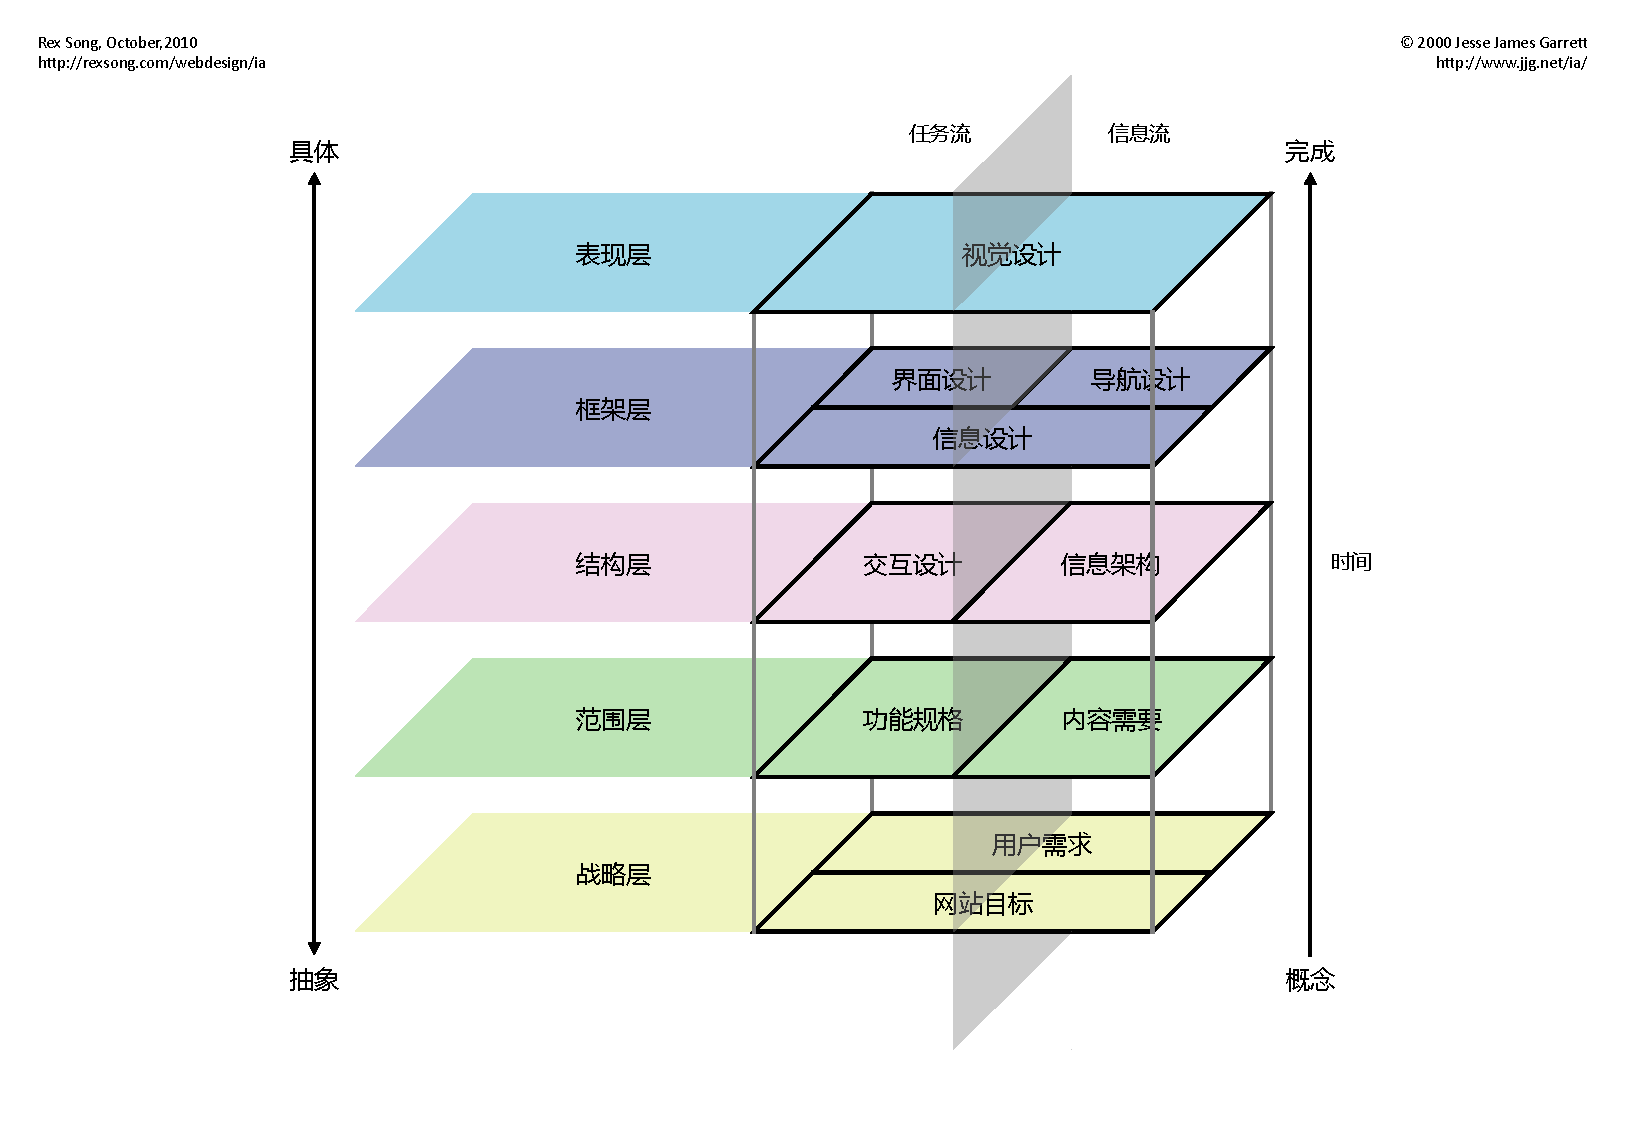
\includegraphics[scale=0.5]{model.pdf}\\
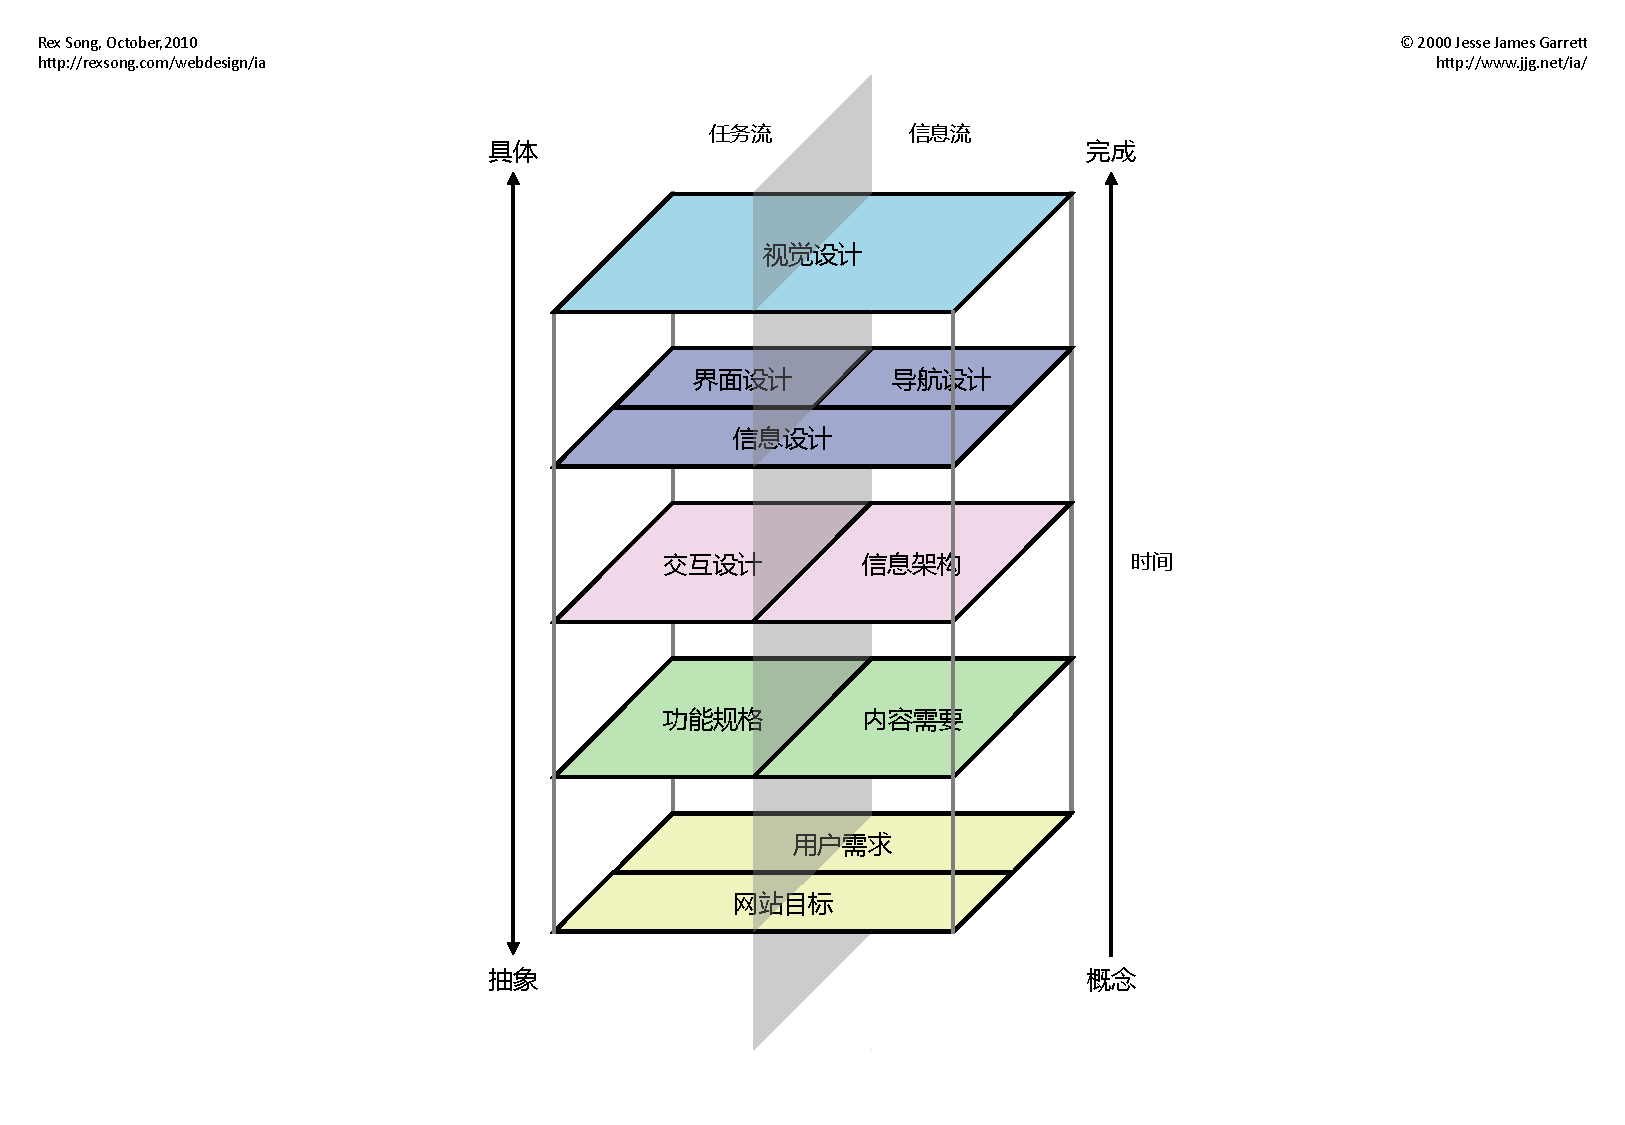
\includegraphics[scale=0.5]{models.pdf}
\end{figure}








\chapter{用十年学习编程}

	\begin{center}著者: Peter Norvig\\ 翻译: Dai Yuwen\cite{tenyears}\end{center}


\section{为何人人都这么着急?}


信步走进任何一家书店,你会看到名为《如何在7天内学会Java》的书,还有各 种各样类似的书: 在几天内或几小时内学会Visual Basic, Windows, Internet等等,一眼望不到 尽头。我在Amazon 上做了如下的 强力检索 :

          \verb|pubdate: after 1992 and title: days and (title: learn or title: teach yourself)|

得到了248个结果。前78个都是计算机类书籍(第79个是 Learn Bengali in 30 days)。我用"hours"替换"days",得到了类似的结果: 更多的253书。前77本是计算机类书籍,第78本是 Teach Yourself Grammar and Style in 24 Hours。在前200本书中,有96\% 是 计算机类书籍。

结论是:要么人们都在急急忙忙地学习计算机,要么计算机比其它任何东西都 容易学。没有书籍教你在几天内学会古典音乐、量子物理,或者是养狗。


让我们分析一下,象一本名为《三天内学会Pascal》的书意味着什么:

\begin{compactitem}
\item 学习: 在三天里,你没有时间写一些重大的程序,并从成功或失败中 得益。你没有时间与有经验的程序员合作,并理解在那样的环境下工作是怎么回 事。一句话,你不会有时间学到太多东西。因此他们只能谈论一些肤浅的东西,而 不是深入的理解。正如亚力山大教皇所说,浅尝辄止是危险的事情。
\item Pascal: 在三天时间里,你可能学会Pascal的语法(如果你 已经学过类似的语言),但你学不到更多的如何使用这些语法的知识。也就是说, 假如你曾是个BASIC程序员,你可以学着用Pascal语法写出BASIC风格的程序,但你不 可能了解Pascal真正的好处(和坏处)。那么关键是什么? Alan Perlis 说过:“一种不改变你编程的思维方式的语言,不值得去学。” 一种可 能的情况是:你必须学一点儿Pascal(或可能性更大的象Visual Basic 或 JavaScript之类),因为你为了完成某种特定的任务,需要与一个现存的工具建立 接口。不过那不是学习如何编程,而是在学习如何完成那个任务。
\item 三天内: 很不幸,这不够,原因由下一节告诉我们。
\end{compactitem}

\section{在十年里学会编程}

研究表明 (Hayes,Bloom)在 任何一种领域内,象下棋、作曲、绘画、钢琴演奏、游泳、网球、以及原子物理学和拓 扑学,等等,要达到专家水平大约都要化十年时间。没有真正的捷径:即使是莫扎 特,4岁时就是音乐神童,13年后才开始写出世界级的作品。在另一方面,披头 士似乎在1964年的Ed Sullivan表演上一炮走红。但他们从1957年就开始表演,在 获得大众青睐后,他们的第一个重大成功,Sgt. Peppers,是1967年发 行的。Samuel Johnson (塞缪尔·约翰逊,英国辞典编纂家及作家)认为要花比十年更长的时间:“在任何领域中出类拔萃都 要用毕生的劳作来取得;它不可能用较低的代价获得。” 而Chaucer(乔叟,英 国诗人)感叹到:“人生短暂,学海无涯。”

这是我为编程成功开出的方子:


\begin{compactitem}
\item 设法对编程感兴趣,并且因为它有趣而编一些程序。确保编程一直充满足够 乐趣,这样你才愿意投入十年宝贵时间。
\item 与其他程序员交流; 阅读其它程序。这比任何书本或训练课程都 重要。
\item 写程序。 最好的学习方式是 从实 践中学习。 用更技术性的话说,“在一个给定的领域内,个人的最大能力不 是自动地由扩展了的经验取得的,但即使是高度有经验的人也可以通过有意识的 努力来提高自己的能力” (p. 366) 和 “最有效的学习需要因人而异的适当难度,目标明确的任务,丰富的信息反 馈,以及重复的机会和错误修正。” (p. 20-21) 此书 Cognition in Practice: Mind,Mathematics,and Culture in Everyday Life 是阐明此观点的令人感兴趣的参考文献。
\item 如果愿意,在大学里呆上4年或更长(在研究生院里)。你会接触到 一些需要学历证明的工作,你会对此领域有更深的理解。如果你不喜欢学校, 你可以(通过一 些贡献)在工作中获得相似的经验。在任何情况下,光啃书本是不够的。Eric Raymond,The New Hacker's Dictionary一书的作者,说过,“计算机科学不能把任何人变成编程 专家,就象光研究刷子和颜料不会使人变成画家一样。” 我雇佣过的最好的程序员 之一仅有高中程度;他做出了许多优秀的 软件,有他自己的新闻组, 而且通过股票期权,他无疑比我富有的多。
\item 和其他程序员一起做项目。在其中的一些项目中作为最好的程序 员; 而在另一些项目中是最差的。当你是最好的,你能测试领导项目的能力,用你 的观点激发别人。当你是最差的,你学习杰出者是怎么做的,了解他们不喜欢做 什么(因为他们吩咐你做事)。
\item 在其他程序员 之后接手项目。使自己理解别人写的程序。 当程序的原作者不在的时候,研究什么需要理解并且修改它。思考如何设计你的 程序以便后来者的维护。
\item 学习至少半打的编程语言。包括一种支持类抽象的语言(象Java 或C++),一种支持函数化抽象的语言(象Lisp或ML),一种支持语法抽象的语 言(象 Lisp),一种支持声明规格说明的语言(象Prolog或C++ 的模板),一种支持 共行程序(coroutine)的语言(象Icon或Scheme),一种支持并行的语言(象Sisal)。
\item 请记住“计算机科学”中有“计算机”一词。了解你的计算机要花多 长时间执行一条指令,从内存中取一个字(有cache),从磁盘中读取连续的字, 和在磁盘中找到新的位置。(答案)
\item 参与一种语言标准化的工作。它可以是ANSI C++委员会, 也可以是决定你周围小范围内的编程风格是应该两个还是四个空格缩进。通 过任何一种方式,你了解到其他人在某种语言中的想法,他们的理解深度,甚至一 些他们这样想的原因。
\item 找到适当的理由尽快地从语言标准化的努力中脱身。

\end{compactitem}

明白了这些,仅从书本中你能得到多少就成了一个问题。在我第一个孩子出生前, 我读了所有的(关于育儿的)How to 书籍,仍然感觉是个手足无措的新手。30个月以后,我 的第二个孩子快要出生了,我回头温习这些书了吗? 没有。相反,我依靠我的个人 经验,它比专家写的数千页书更有用和可靠。

Fred Brooks在他的随笔 《没有银弹》 中定出了一个寻找优秀软件设计者的三步计划:

\begin{compactenum}
\item 尽可能早地,有系统地识别顶级的设计人员。
\item 为设计人员指派一位职业导师,负责他们技术方面的成长,仔细地为他们规划 职业生涯。
\item 为成长中的设计人员提供相互交流和学习的机会。
\end{compactenum}

此计划假设某些人已经具备了杰出设计者的必要才能; 要做的只是如何恰当地诱 导他们。 Alan Perlis 说得更简明扼要:“每个人都能被教会雕刻:对米开朗其罗而言, 反倒是告诉他哪些事不要做。同样的道理也适用于优秀的程序员。”
所以尽管买那本Java的书吧。你可能会从中学到点儿东西。但作为一个程序员,你不会在 几天内或24小时内,哪怕是几个月内改变你的人生,或你实际的水平。

\section{参考文献}

Bloom, Benjamin (ed.) \href{http://www.amazon.com/exec/obidos/ASIN/034531509X}{Developing Talent in Young People}, Ballantine, 1985.

Brooks, Fred, \href{http://citeseer.nj.nec.com/context/7718/0}{No Silver Bullets}, IEEE Computer, vol. 20, no. 4, 1987, p. 10-19.

Hayes, John R., \href{http://www.amazon.com/exec/obidos/ASIN/0805803092}{Complete Problem Solver} Lawrence Erlbaum, 1989.

Lave, Jean, \href{http://www.amazon.com/exec/obidos/ASIN/0521357349}{Cognition in Practice: Mind, Mathematics, and Culture in Everyday Life}, Cambridge University Press, 1988.

\section{答案}

2001年夏天典型的1GHz PC的各种操作要花的时间

\begin{tabular}{|l|l|}
\hline
执行一条指令	 &1 nsec = (1/1,000,000,000) sec\\
\hline
从L1 cache memory 中取一个字&	 2 nsec\\
\hline
从内存中取一个字	 &10 nsec\\
\hline
从磁盘的连续位置取一个字	 &200 nsec\\
\hline
从磁盘的新位置取一个字(seek)	& 8,000,000nsec = 8msec\\
\hline
\end{tabular}

\section{附录:语言的选择}

不少人问我,他们首先该学哪种编程语言。没有绝对的答案,不过请考虑以下几 点:


\begin{compactitem}
\item 用你的朋友的。当被问起“我该用哪种操作系统,Windows,Unix, 还是Mac?”,我总是回答:“你朋友用什么,你就用什么。” 你从朋友那能学 到知识,这种优势可以抵销不同操作系统或语言之间本质的差异。也考虑你将来 的朋友:程序员社区 — 你将成为它的一部分如果你继续往前走的话。你选择的 语言是否有一个成长中的社区,还是人数不多、即将消亡? 有没有书籍、网站、 在线论坛回答你的问题? 你喜欢论坛里的那些人吗?
\item Keep it simple, stupid. 象C++和Java这样的语言是为经验丰富的 程序员组成的团队进行专业开发而设计的,他们专注于代码运行时的效率。因此, 这些语言有些部分非常复杂。 而你关注的是如何编程,不需要那些复杂性。你 需要的是这样的语言: 对单个的编程新手来说,它易学易记。
\item 练习。你偏爱哪种学弹钢琴的方式:通常的交互式的方式,你一 按下琴键就能听到音符;还是“批量”模式,你只有弹完整首曲子才能听到音符? 显然,用交互模式学习弹钢琴更容易些,编程也一样。坚持用交互模式学习并使 用一种语言。

\end{compactitem}

有了上面的准则,我推荐的第一个编程语言是Python或Scheme。因人而异,还有其它 好的选择。如果你的年纪是10岁以下,你可能更喜欢Alice。关键是你要选择并开始实践。

\section{附录:书籍和其它资源}


不少人问我,他们该从什么书籍或网页开始学起。我重申“仅从书本里学习是不 够的。” 但我还是推荐:

\begin{compactitem}
\item Scheme: \href{http://www.amazon.com/gp/product/0262011530}{Structure and Interpretation of Computer Programs (Abelson \& Sussman)}可能是最好 的计算机科学的入门书,而且它的确把讲授编程作为理解计算机科学的一种方法。 但它具有挑战性,会让许多通过其它方式可能成功的人望而却步。
\item Scheme: \href{http://www.amazon.com/gp/product/0262062186}{How to Design Programs (Felleisen et al.)}是关于如何用一种优美的、函数化的方式设 计程序的最好的书之一。
\item Python: \href{http://www.amazon.com/gp/product/1887902996}{Python Programming: An Intro to CS (Zelle)}是优秀的Python入门指导。
\item Python: \href{http://python.org/}{Python.org}上有许多在线\href{http://wiki.python.org/moin/BeginnersGuide}{指导}。
\item Oz: \href{http://www.amazon.com/gp/product/0262220695}{Concepts, Techniques, and Models of Computer Programming (Van Roy \& Haridi)} 被视为Abelson \& Sussman的当代继承者。它是对编程的高层次概念的巡视。 涉及的范围比Abelson \& Sussman更广,同时可能更容易学习和跟进。 它用了叫 做Oz的语言,不太知名,却可以作为学习其它语言的基础。
\end{compactitem}

\section{脚注}

This page also available in Japanese translation thanks to Yasushi Murakawa, in Spanish translation thanks to Carlos Rueda and in German translation thanks to Stefan Ram.

T. Capey points out that the Complete Problem Solver page on Amazon now has the "Teach Yourself Bengali in 21 days" and "Teach Yourself Grammar and Style" books under the "Customers who shopped for this item also shopped for these items" section. I guess that a large portion of the people who look at that book are coming from this page.

\begin{flushright}
\href{http://www.norvig.com/index.html}{Peter Norvig(Copyright 2001)}
\end{flushright}


\vspace{20pt}

\begin{center}\textbf{用十年学习编程}\end{center}
	

出处:网络

	

前几天,系里排课,有教师讲“语言课(C++、JAVA等)随便找个老师就能上”。我哑然,如果计算机专业的老师都这样,我不知,会教出什么样的学生来。

今天浏览互联网,无意看到下面的文章,大家看后可以点评。以下是译文与原文。


为什么每个人都急不可耐?

走进任何一家书店,你会看见《Teach Yourself Java in 7 Days》(7天Java无师自通)的旁边是一长排看不到尽头的类似书籍,它们要教会你Visual Basic、Windows、Internet等等,而只需要几天甚至几小时。我在Amazon.com上进行了如下搜索:

pubdate: after 1992 and title: days and (title: learn or title: teach yourself)

(出版日期:1992年后 and 书名:天 and (书名:学会 or 书名:无师自通))

我一共得到了248个搜索结果。前面的78个是计算机书籍(第79个是《Learn Bengali in 30 days》,30天学会孟加拉语)。我把关键词“days”换成“hours”,得到了非常相似的结果:这次有253本书,头77本是计算机书籍,第78本是《Teach Yourself Grammar and Style in 24 Hours》(24小时学会文法和文体)。头200本书中,有96\%是计算机书籍。

结论是,要么是人们非常急于学会计算机,要么就是不知道为什么计算机惊人地简单,比任何东西都容易学会。没有一本书是要在几天里教会人们欣赏贝多芬或者量子物理学,甚至怎样给狗打扮。

让我们来分析一下像《Learn Pascal in Three Days》(3天学会Pascal)这样的题目到底是什么意思:

\begin{compactitem}
\item 学会:在3天时间里,你不够时间写一些有意义的程序,并从它们的失败与成功中学习。你不够时间跟一些有经验的程序员一起工作,你不会知道在那样的环境中是什么滋味。简而言之,没有足够的时间让你学到很多东西。所以这些书谈论的只是表面上的精通,而非深入的理解。如Alexander Pope(英国诗人、作家,1688-1744)所言,一知半解是危险的(a little learning is a dangerous thing)
\item Pascal:在3天时间里你可以学会Pascal的语法(如果你已经会一门类似的语言),但你无法学到多少如何运用这些语法。简而言之,如果你是,比如说一个Basic程序员,你可以学会用Pascal语法写出Basic风格的程序,但你学不到Pascal真正的优点(和缺点)。那关键在哪里?Alan Perlis(ACM第一任主席,图灵奖得主,1922-1990)曾经说过:“如果一门语言不能影响你对编程的想法,那它就不值得去学”。另一种观点是,有时候你不得不学一点Pascal(更可能是Visual Basic和javascript之类)的皮毛,因为你需要接触现有的工具,用来完成特定的任务。但此时你不是在学习如何编程,你是在学习如何完成任务。
\item 3天:不幸的是,这是不够的,正如下一节所言。
\end{compactitem}

\textbf{10年编程无师自通}


一些研究者(Hayes、Bloom)的研究表明,在许多领域,都需要大约10 年时间才能培养出专业技能,包括国际象棋、作曲、绘画、钢琴、游泳、网球,以及神经心理学和拓扑学的研究。似乎并不存在真正的捷径:即使是莫扎特,他4岁就显露出音乐天才,在他写出世界级的音乐之前仍然用了超过13年时间。再看另一种音乐类型的披头士,他们似乎是在1964年的Ed Sullivan节目中突然冒头的。但其实他们从1957年就开始表演了,即使他们很早就显示出了巨大的吸引力,他们第一次真正的成功——Sgt. Peppers——也要到1967年才发行。Samuel Johnson(英国诗人)认为10 年还是不够的:“任何领域的卓越成就都只能通过一生的努力来获得;稍低一点的代价也换不来。”(Excellence in any department can be attained only by the labor of a lifetime; it is not to be purchased at a lesser price.) 乔叟(Chaucer,英国诗人,1340-1400)也抱怨说:“生命如此短暂,掌握技艺却要如此长久。”(the lyf so short, the craft so long to lerne.)

下面是我在编程这个行当里获得成功的处方:

\begin{compactitem}
\item 对编程感兴趣,因为乐趣而去编程。确定始终都能保持足够的乐趣,以致你能够将10年时间投入其中。

\item 跟其他程序员交谈;阅读其他程序。这比任何书籍或训练课程都更重要。

\item 编程。最好的学习是从实践中学习。用更加技术性的语言来讲,“个体在特定领域最高水平的表现不是作为长期的经验的结果而自动获得的,但即使是非常富有经验的个体也可以通过刻意的努力而提高其表现水平。”(p. 366),而且“最有效的学习要求为特定个体制定适当难度的任务,有意义的反馈,以及重复及改正错误的机会。”(p. 20-21)《Cognition in Practice: Mind, Mathematics, and Culture in Everyday Life》(在实践中认知:心智、数学和日常生活的文化)是关于这个观点的一本有趣的参考书。

\item 如果你愿意,在大学里花上4年时间(或者再花几年读研究生)。这能让你获得一些工作的入门资格,还能让你对此领域有更深入的理解,但如果你不喜欢进学校,(作出一点牺牲)你在工作中也同样能获得类似的经验。在任何情况下,单从书本上学习都是不够的。“计算机科学的教育不会让任何人成为内行的程序员,正如研究画笔和颜料不会让任何人成为内行的画家”, Eric Raymond,《The New Hacker's Dictionary》(新黑客字典)的作者如是说。我曾经雇用过的最优秀的程序员之一仅有高中学历;但他创造出了许多伟大的软件,甚至有讨论他本人的新闻组,而且股票期权让他达到我无法企及的富有程度(译注:指Jamie Zawinski,Xemacs和Netscape的作者)。

\item 跟别的程序员一起完成项目。在一些项目中成为最好的程序员;在其他一些项目中当最差的一个。当你是最好的程序员时,你要测试自己领导项目的能力,并通过你的洞见鼓舞其他人。当你是最差的时候,你学习高手们在做些什么,以及他们不喜欢做什么(因为他们让你帮他们做那些事)。

\item 接手别的程序员完成项目。用心理解别人编写的程序。看看在没有最初的程序员在场的时候理解和修改程序需要些什么。想一想怎样设计你的程序才能让别人接手维护你的程序时更容易一些。

\item 学会至少半打编程语言。包括一门支持类抽象(class abstraction)的语言(如Java或C++),一门支持函数抽象(functional abstraction)的语言(如Lisp或ML),一门支持句法抽象(syntactic abstraction)的语言(如Lisp),一门支持说明性规约(declarative specification)的语言(如Prolog或C++模版),一门支持协程(coroutine)的语言(如Icon或Scheme),以及一门支持并行处理(parallelism)的语言(如Sisal)。

\item 记住在“计算机科学”这个词组里包含“计算机”这个词。了解你的计算机执行一条指令要多长时间,从内存中取一个word要多长时间(包括缓存命中和未命中的情况),从磁盘上读取连续的数据要多长时间,定位到磁盘上的新位置又要多长时间。(答案在这里。)

\item 尝试参与到一项语言标准化工作中。可以是ANSI C++委员会,也可以是决定自己团队的编码风格到底采用2个空格的缩进还是4个。不论是哪一种,你都可以学到在这门语言中到底人们喜欢些什么,他们有多喜欢,甚至有可能稍微了解为什么他们会有这样的感觉。

\item 拥有尽快从语言标准化工作中抽身的良好判断力。

\end{compactitem}



抱着这些想法,我很怀疑从书上到底能学到多少东西。在我第一个孩子出生前,我读完了所有“怎样……”的书,却仍然感到自己是个茫无头绪的新手。30个月后,我第二个孩子出生的时候,我重新拿起那些书来复习了吗?不。相反,我依靠我自己的经验,结果比专家写的几千页东西更有用更靠得住。

Fred Brooks在他的短文《No Silver Bullets》(没有银弹)中确立了如何发现杰出的软件设计者的三步规划:

\begin{compactenum}
\item 尽早系统地识别出最好的设计者群体。
\item 指派一个事业上的导师负责有潜质的对象的发展,小心地帮他保持职业生涯的履历。
\item 让成长中的设计师们有机会互相影响,互相激励。
\end{compactenum}



这实际上是假定了有些人本身就具有成为杰出设计师的必要潜质;要做的只是引导他们前进。Alan Perlis说得更简洁:“每个人都可以被教授如何雕塑;而对米开朗基罗来说,能教给他的倒是怎样能够不去雕塑。杰出的程序员也一样”。

所以尽管去买那些Java书;你很可能会从中找到些用处。但你的生活,或者你作为程序员的真正的专业技术,并不会因此在24小时、24天甚至24个月内发生真正的变化。

出处:网络

\bibliographystyle{plainnat}
\bibliography{gk}
\clearpage


\chapter{理论计算机科学漫谈}


******************************************************************
  
版权声明:本文作者sir系旅美学人、南京大学校友。 

为了学术或 教育的(非营利)目的,在保留本版权

声明的情况下,您可以自由 转载本文的电子版。

如果您要在传统媒体上转载此文,请与南京大学

小百合BBS站上的网友sir联系。 

****************************************************************** 




\begin{center}\textbf{理论计算机科学漫谈}\end{center}




早就答应russel的,今天有点时间,把欠债还上。 

计算机科学和数学的关系有点奇怪。二三十年以前,计算机科学基本上还是数学的一个分支。而现在,计算机科学拥有广泛的研究领域和众多的研究人员,在很多方面反过来推动数学发展,从某种意义上可以说是孩子长得比妈妈还高了。 

但不管怎么样,这个孩子身上始终流着母亲的血液。这血液是the mathematical underpinning of computer science(计算机科学的数学基础),-- 也就是理论计算机科学。 

现代计算机科学和数学的另一个交叉是计算数学/数值分析/科学计算,传统上不包含在理论计算机科学以内。所以本文对计算数学全部予以忽略。 

最常和理论计算机科学放在一起的一个词是什么? 答:离散数学。这两者的关系是如此密切,以至于它们在不少场合下成为同义词。 

传统上,数学是以分析为中心的。数学系的同学要学习三四个学期的数学分析,然后是复变,实变,泛函等等。实变和泛函被很多人认为是现代数学的入门。在物理,化学,工程上应用的,也以分析为主。 

随着计算机科学的出现,一些以前不太受到重视的数学分支突然重要起来。人们发现,这些分支处理的数学对象与传统的分析有明显的区别:分析研究的对象是连续的,因而微分,积分成为基本的运算;而这些分支研究的对象是离散的,因而很少有机会进行此类的计算。人们从而称这些分支为“离散数学”。“离散数学”的名字越来越响亮,最后导致以分析为中心的传统数学分支被相对称为“连续数学”。 

离散数学经过几十年发展,基本上稳定下来。一般认为,离散数学包含以下学科: 

\begin{compactenum}
\item 集合论,数理逻辑与元数学。这是整个数学的基础,也是计算机科学的基础。 
\item 图论,算法图论;组合数学,组合算法。计算机科学,尤其是理论计算机科学的核心是算法,而大量的算法建立在图和组合的基础上 
\item 抽象代数。代数是无所不在的,本来在数学中就非常重要。在计算机科学中,人们惊讶地发现代数竟然有如此之多的应用。 
\end{compactenum}



但是,理论计算机科学仅仅就是在数学的上面加上“离散”的帽子这么简单吗?一直到大约十几年前,终于有一位大师告诉我们:不是。 

D.E.Knuth(他有多伟大,我想不用我废话了)在Stanford开设了一门全新的课程Concrete Mathematics。 Concrete这个词在这里有两层含义: 

第一,针对abstract而言。Knuth认为,传统数学研究的对象过于抽象,导致对具体的问题关心不够。他抱怨说,在研究中他需要的数学往往并不存在,所以他只能自己去创造一些数学。为了直接面向应用的需要,他要提倡“具体”的数学。 

在这里我做一点简单的解释。例如在集合论中,数学家关心的都是最根本的问题--公理系统的各种性质之类。而一些具体集合的性质,各种常见集合,关系,映射都是什么样的,数学家觉得并不重要。然而,在计算机科学中应用的,恰恰就是这些具体的东西。Knuth能够首先看到这一点,不愧为当世计算机第一人。 

第二,Concrete是Continuous(连续)加上discrete (离散)。不管连续数学还是离散数学,都是有用的数学! 

前面主要是从数学角度来看的。从计算机角度来看,理论计算机科学目前主要的研究领域包括:可计算性理论,算法设计与复杂性分析,密码学与信息安全,分布式计算理论,并行计算理论,网络理论,生物信息计算,计算几何学,程序语言理论等等。这些领域互相交叉,而且新的课题在不断提出,所以很难理出一个头绪来。下面随便举一些例子。 

由于应用需求的推动,密码学现在成为研究的热点。密码学建立在数论(尤其是计算数论),代数,信息论,概率论和随机过程的基础上,有时也用到图论和组合学等。 

很多人以为密码学就是加密解密,而加密就是用一个函数把数据打乱。这就大错特错了。现代密码学至少包含以下层次的内容: 

第一,密码学的基础。例如,分解一个大数真的很困难吗?能否有一般的工具证明协议正确? 

第二,密码学的基本课题。例如,比以前更好的单向函数,签名协议等。 

第三,密码学的高级问题。例如,零知识证明的长度,秘密分享的方法。 

第四,密码学的新应用。例如,数字现金,叛徒追踪等。 

在分布式系统中,也有很多重要的理论问题。例如,进程之间的同步,互斥协议。一个经典的结果是:在通信信道不可靠时,没有确定型算法能实现进程间协同。所以,改进TCP三次握手几乎没有意义。例如时序问题。常用的一种序是因果序,但因果序直到不久前才有一个理论上的结果.... 

例如,死锁没有实用的方法能完美地对付。  

例如,...... 

  

关于死锁 Re: 理论计算机科学漫谈(6) 
  

我简单地觉得与“熵”这个东西有关. 没有这么复杂。关键在效率:对付死锁的方法,例如死锁检测,都非常严重地减低效率,以至于得不尝失,因为死锁并不是一种经常出现的现象。所以在全局上,一般都用所谓“鸵鸟算法”,也就是假装什么都不会发生。在局部上,例如你要设计一个访问共享数据的算法,那么你就要证明你的算法在局部上是deadlock free。至于它会不会导致全局的死锁,就烦不了许多了。 





发信人: sir (sir), 信区: Mathematics. 本篇人气: 8984

标  题: 理论计算机科学漫谈(1)\cite{tcs1}

发信站: 南大小百合 (Thu Nov 30 11:08:08 2000) , 转信

\textbf{理论计算机科学漫谈(1)}



早就答应russel的,今天有点时间,把欠债还上。

计算机科学和数学的关系有点奇怪。二三十年以前,计算机科学基本上还是数学的一个分支。而现在,计算机科学拥有广泛的研究领域和众多的研究人员,在很多方面反过来推动数学发展,从某种意义上可以说是孩子长得比妈妈还高了。

但不管怎么样,这个孩子身上始终流着母亲的血液。这血液是the mathematical underpinning of computer science(计算机科学的数学基础),-- 也就是理论计算机科学。

现代计算机科学和数学的另一个交叉是计算数学/数值分析/科学计算,传统上不包含在理论计算机科学以内。所以本文对计算数学全部予以忽略。

\textbf{理论计算机科学漫谈(2)}

发信人: sir (sir), 信区: Mathematics. 本篇人气: 1950

标  题: 理论计算机科学漫谈(2)\cite{tcs2}

发信站: 南大小百合 (Thu Nov 30 11:23:19 2000) , 转信

最常和理论计算机科学放在一起的一个词是什么?答:离散数学。这两者的关系是如此密切,以至于它们在不少场合下成为同义词。

传统上,数学是以分析为中心的。数学系的同学要学习三四个学期的数学分析,然后是复变,实变,泛函等等。实变和泛函被很多人认为是现代数学的入门。在物理,化学,工程上应用的,也以分析为主。

随着计算机科学的出现,一些以前不太受到重视的数学分支突然重要起来。人们发现,这些分支处理的数学对象与传统的分析有明显的区别:分析研究的对象是连续的,因而微分,积分成为基本的运算;而这些分支研究的对象是离散的,因而很少有机会进行此类的计算。人们从而称这些分支为“离散数学”。“离散数学”的名字越来越响亮,最后导致以分析为中心的传统数学分支被相对称为“连续数学”。

\textbf{理论计算机科学漫谈(3)}


发信人: sir (sir), 信区: Mathematics. 本篇人气: 1549

标  题: 理论计算机科学漫谈(3)\cite{tcs3}

发信站: 南大小百合 (Thu Nov 30 11:30:37 2000) , 转信


离散数学经过几十年发展,基本上稳定下来。一般认为,离散数学包含以下学科:

1) 集合论,数理逻辑与元数学。这是整个数学的基础,也是计算机科学的基础。

2) 图论,算法图论;组合数学,组合算法。计算机科学,尤其是理论计算机科学的核心是算法,而大量的算法建立在图和组合的基础上。

3) 抽象代数。代数是无所不在的,本来在数学中就非常重要。在计算机科学中,人们惊讶地发现代数竟然有如此之多的应用。


\textbf{理论计算机科学漫谈(4)}

发信人: sir (sir), 信区: Mathematics. 本篇人气: 1381

标  题: 理论计算机科学漫谈(4)\cite{tcs4}

发信站: 南大小百合 (Thu Nov 30 11:44:35 2000) , 转信


但是,理论计算机科学仅仅就是在数学的上面加上“离散”的帽子这么简单吗?一直到大约十几年前,终于有一位大师告诉我们:不是。

D.E.Knuth(他有多伟大,我想不用我废话了)在Stanford开设了一门全新的课程Concrete Mathematics。 Concrete这个词在这里有两层含义:

第一,针对abstract而言。Knuth认为,传统数学研究的对象过于抽象,导致对具体的问题关心不够。他抱怨说,在研究中他需要的数学往往并不存在,所以他只能自己去创造一些数学。为了直接面向应用的需要,他要提倡“具体”的数学。

在这里我做一点简单的解释。例如在集合论中,数学家关心的都是最根本的问题--公理系统的各种性质之类。而一些具体集合的性质,各种常见集合,关系,映射都是什么样的,数学家觉得并不重要。然而,在计算机科学中应用的,恰恰就是这些具体的东西。Knuth能够首先看到这一点,不愧为当世计算机第一人。

第二,Concrete是Continuous(连续)加上discrete(离散)。不管连续数学还是离散数学,都是有用的数学!


\textbf{理论计算机科学漫谈(5)}



发信人: sir (sir), 信区: Mathematics. 本篇人气: 1269

标  题: 理论计算机科学漫谈(5)\cite{tcs5}

发信站: 南大小百合 (Thu Nov 30 12:09:50 2000) , 转信


前面主要是从数学角度来看的。从计算机角度来看,理论计算机科学目前主要的研究领域包括:可计算性理论,算法设计与复杂性分析,密码学与信息安全,分布式计算理论,并行计算理论,网络理论,生物信息计算,计算几何学,程序语言理论等等。这些领域互相交叉,而且新的课题在不断提出,所以很难理出一个头绪来。

下面随便举一些例子。

由于应用需求的推动,密码学现在成为研究的热点。密码学建立在数论(尤其是计算数论),代数,信息论,概率论和随机过程的基础上,有时也用到图论和组合学等。

很多人以为密码学就是加密解密,而加密就是用一个函数把数据打乱。这就大错特错了。

现代密码学至少包含以下层次的内容:

第一,密码学的基础。例如,分解一个大数真的很困难吗?能否有一般的工具证明协议正确?

第二,密码学的基本课题。例如,比以前更好的单向函数,签名协议等。

第三,密码学的高级问题。例如,零知识证明的长度,秘密分享的方法。

第四,密码学的新应用。例如,数字现金,叛徒追踪等。

\textbf{理论计算机科学漫谈(6)}

发信人: sir (sir), 信区: Mathematics. 本篇人气: 1292

标  题: 理论计算机科学漫谈(6)\cite{tcs6}

发信站: 南大小百合 (Thu Nov 30 12:18:32 2000) , 转信



在分布式系统中,也有很多重要的理论问题。

例如,进程之间的同步,互斥协议。一个经典的结果是:在通信信道不可靠时,没有确定型算法能实现进程间协同。所以,改进TCP三次握手几乎没有意义。

例如时序问题。常用的一种序是因果序,但因果序直到不久前才有一个理论上的结果....
..

例如,死锁没有实用的方法能完美地对付。

例如,......

【 在 pie (燃烧吧,小宇宙!) 的大作中提到: 】

: 【 在 probe (农民) 的大作中提到: 】

: 我简单地觉得与“熵”这个东西有关

没有这么复杂。关键在效率:对付死锁的方法,例如死锁检测,都非常严重地减低效率,以至于得不尝失,因为死锁并不是一种经常出现的现象。所以在全局上,一般都用所谓“鸵鸟算法”,也就是假装什么都不会发生。在局部上,例如你要设计一个访问共享数据的算法,那么你就要证明你的算法在局部上是deadlock free。至于它会不会导致全局的死锁,就烦不了许多了。





\textbf{关于计算机学习}

发信人: sir (sir), 信区: Mathematics. 本篇人气: 763

标  题: 回答pie关于计算机学习

发信站: 南大小百合 (Fri Dec  1 07:28:49 2000) , 转信

其实,我也是从那个迷茫的年代里走过来的。计算机是一个新兴学科,亦理亦工,其教学在国际上都不成熟,更不用说与国际水平差距很大的国内教学了。

我个人的看法:

首先,如果要做research,就要把基础打好。数学是计算机系学生的内功,学好数学,无论做什么都胆子壮一点。我们以前学习的那一点数学远远不够。至少,下面列举的数学是重要的:代数(群环域,布尔代数和多项式理论),数论和计算数论,概率论,数理统计和随机过程,图论和算法图论,组合分析,数值分析,数理逻辑和集合论,数学基础,信息论,博弈论,线性和非线性规划。

随便举个例子:学数字通信时,会学到很多编码。你感到很枯燥,也难以记住,更不知道它有什么用处。但事实上,这些编码全部都有深刻的代数背景。如果你懂得其原理,就会感到学术的美妙。

其次,大量使用hack是工程学科的特点。无论你是否做研究,你都算是一个工程师。你必须理解,hack总是在理论不起作用时让我们避免麻烦。hack的背景是经验,所以你刚接触时很难理解它,即使你聪明过人。对策是多读相关的背景材料和多动手实践,尤其是动手。

举例说:你能理解为什么IP路由一定要搞成这样?看看RFC,再自己动手编点程序试验一下。我认识的师兄中里就有超级大牛,他如何成为大牛的?不就是这样一点点积累出来的?
你如果捧着课本想,永远也想不通。

第三,天才的想法总是少数,大部份工作是平凡的。但是,天才的想法往往是在大量平凡工作的基础上产生的。我看别人的文章,总觉得naive。但三篇naive的文章积累起来,其进步就不是你随便能想到的。做工作要从最基本的着手。

我的看法不见得正确。欢迎列位高手指正。



: 这里我有一点感慨:

: 虽然读了几年大学,我却不知道应该学什么。

: 因为我所见的所谓knowledge实在是一系列的technique和trick

: Sience是什么?我渴求而又看不见.

: 阿Sir学长,Is naivete necessary in the research for science?

: I am quite curious.

\chapter{胡侃学习(理论)计算机}


******************************************************************  

版权声明:本文作者sir系旅美学人、南京大学校友。 

为了学术或 教育的(非营利)目的,在保留本版权

声明的情况下,您可以自由 转载本文的电子版。

如果您要在传统媒体上转载此文,请与南京大学

小百合BBS站上的网友sir联系。 

****************************************************************** 

出处:http://bbs.sjtu.edu.cn/bbstcon?board=CS\&reid=1178579072


我也来冒充一回高手,谈谈学习计算机的一点个人体会。由于我是做理论的,所以先着重谈谈理论。 

记得当年大一,刚上本科的时候,每周六课时数学分析,六课时高等代数,天天作业不断(那时是六日工作制)。颇有些同学惊呼走错了门:咱们这到底念的是什么系?不错,你没走错门,这就是(当时的)南大计算机系。系里的传统是培养做学术研究,尤其是理论研究的人。而计算机的理论研究,说到底了就是数学,虽然也许是正统数学家眼里非主流的数学。 

数学分析这个东东,咱们学计算机的人对它有很复杂的感情。爱它在于它是第一门,也是学分最多的一门数学课,又长期为考研课程--94以前可以选考数学分析与高等代数,以后则并轨到著名的所谓“工科数学一”。其重要性可见一斑。恨它则在于它好象难得有用到的机会,而且思维跟咱们平常做的这些离散/有限的工作截然不同。当年出现的怪现象是:计算机系学生的高中数学基础在全校数一数二(希望没有冒犯其它系的同学),教学课时数也仅次于数学系,但学完之后的效果却几乎是倒数第一。其中原因何在,发人深思。 

我个人的浅见是:计算机类的学生,对数学的要求固然跟数学系不同,跟物理类差别则更大。通常非数学专业的所谓“高等数学”,无非是把数学分析中较困难的理论部分删去,强调套用公式计算而已。而对计算机系来说,数学分析里用处最大的恰恰是被删去的理论部分。说得难听一点,对计算机系学生而言,追求算来算去的所谓“工科数学一”已经彻底地走进了魔道。记上一堆曲面积分的公式,难道就能算懂了数学分析? 

中文的数学分析书,一般都认为以北大张筑生老师的“数学分析新讲”为最好。我个人认为南大数学系的“数学分析教程”也还不错,至少属于典型的南大风格,咱们看着亲切。随便学通哪一本都行。万一你的数学实在太好,这两本书都吃不饱,那就去看菲赫金哥尔茨的“微积分学教程”好了--但我认为没什么必要,毕竟你不想转到数学系去。 

吉米多维奇的“数学分析习题集”也基本上是计算型的东东。如果你打算去考那个什么“工科数学一”,可以做一做。否则,不做也罢。 

中国的所谓高等代数,就等于线性代数加上一点多项式理论。我以为这有好的一面,因为可以让学生较早感觉到代数是一种结构,而非一堆矩阵翻来覆去。当年我们用林成森,盛松柏两位老师编的“高等代数”,感觉相当舒服,我直到现在还保留着教材。此书相当全面地包含了关于多项式和线性代数的基本初等结果,同时还提供了一些有用的比较深的内容,如Sturm序列,Shermon-Morrison公式,广义逆矩阵等等。可以说,作为本科生如能吃透此书,就可以算高手。后来它得以在南大出版社出版,可惜好象并轨以后就没有再用了。 

国内较好的高等代数教材还有清华计算机系用的那本,清华出版社出版,书店里多多,一看就知道。特点嘛,跟南大那本差不太多。 

但以上两本书也不能说完美无缺。从抽象代数的观点来看,高等代数里的结果不过是代数系统性质的一些例子而已。莫宗坚先生的“代数学”里,对此进行了深刻的讨论。然而莫先生的书实在深得很,作为本科生恐怕难以接受,不妨等到自己以后成熟了一些再读。 

概率论与数理统计这门课很重要,可惜少了些东西。 

少了的东西是随机过程。到毕业还没有听说过Markov过程,此乃计算机系学生的耻辱。没有随机过程,你怎么分析网络和分布式系统?怎么设计随机化算法和协议?据说清华计算机系开有“随机数学”,早就是必修课。人家可是工科学校,作为自以为“理科计算机系”出身的人,我感到惭愧。 

另外,离散概率对计算机系学生来说有特殊的重要性。现在,美国已经有些学校开设了单纯的“离散概率论”课程,干脆把连续概率删去,把离散概率讲深些。我们不一定要这么做,但应该更加强调离散概率是没有疑问的。 

计算方法是最后一门由数学系给我们开的课。一般学生对这门课的重视程度有限,以为没什么用。其实,做图形图像可离不开它。而且,在很多科学工程中的应用计算,都以数值的为主。 

这门课有两个极端的讲法:一个是古典的“数值分析”,完全讲数学原理和算法;另一个是现在日趋流行的“科学与工程计算”,干脆教学生用软件包编程。南大数学系的几位老师做了件大好事,把前者的一本极为经典的教材翻译出版了:德国Stoer的“数值分析引论”。如果你能学会此书中最浅显的三分之一,就算没有白上过计算方法这门课!而后一种讲法似乎国内还没有跟上潮流?不过,只要你有机会在自己的电脑上装个matlab之类,完全可以无师自通。 

本系里,通常开一门离散数学,包括集合论,图论,和抽象代数,另外再单开一门数理逻辑。这样安排,主要由于南大的逻辑传统:系里很多老师都算莫先生的门人,就连孙先生都是逻辑专业出身(见孙先生自述)。 

不过,这么多内容挤在离散数学一门课里,是否时间太紧了点?另外,计算机系学生不懂组合和数论,也是巨大的缺陷。要做理论,不懂组合或者数论吃亏可就太大了。 

从理想的状态来看,最好分开六门课:集合,逻辑,图论,组合,代数,数论。这个当然不现实,因为没那么多课时。也许将来可以开三门课:集合与逻辑,图论与组合,代数与数论。 

不管课怎么开,学生总一样要学。下面分别谈谈上面的三组内容。 

古典集合论,北师大出过一本“基础集合论”不错。南大出版朱梧(木贾)老师的“集合论导引”也许观点更高些,但他的书形式化得太厉害,念起来吃力。 

数理逻辑,莫先生的书自然是经典。然而我们也不得不承认,此书年代久远,光读它恐怕不够。尤其是命题/谓词演算本身有好多种不同的讲法,多看几家能大大开阔自己的视野。例如陆钟万老师的“面向计算机科学的数理逻辑”就不错。朱老师也著有“数理逻辑教程”一书,但也同样读起来费力些。 

总的来说,学集合/逻辑起手不难,但越往后越感觉深不可测。建议有兴趣的同学读读朱老师的“数学基础引论”--此书有点时间简史的风格,讲到精彩处,所谓“天花乱坠,妙雨缤纷”,令人目不暇接。读完以后,你对这些数学/哲学中最根本的问题有了个大概了解,也知道了山有多高,海有多深。 

学完以上各书之后,如果你还有精力兴趣进一步深究,那么可以试一下GTM系列中的"Introduction to Axiomatic Set Theory"和"A Course of Mathematical Logic"。这两本都有世界图书的引进版。你如果能搞定这两本,可以说在逻辑方面真正入了门,也就不用再浪费时间听我瞎侃了。:) 

据说全中国最多只有三十个人懂图论(当年上课时陈道蓄老师转引张克民老师的话)。此言不虚。图论这东东,技巧性太强,几乎每题都有一个独特的方法,让人头痛。不过这也正是它魅力所在:只要你有创造性,它就能给你成就感。所以学图论没什么好说的,做题吧。 

国内的图论书中,王树禾老师的“图论及其算法”非常成功。一方面,其内容在国内教材里算非常全面的。另一方面,其对算法的强调非常适合计算机系(本来就是科大计算机系教材)。有了这本书为主,再参考几本翻译的,如Bondy\&Murty的“图论及其应用”,邮电出版社翻译的“图论和电路网络”等等,就马马虎虎,对本科生足够了。 

再进一步,世界图书引进有GTM系列的"ModernGraph Theory"。此书确实经典!国内好象还有一家出版了个翻译版。不过,学到这个层次,还是读原版好。搞定这本书,也标志着图论入了门,呵呵。组合感觉没有太适合的国产书。还是读Graham和Knuth 等人合著的经典“具体数学”吧,有翻译版,西电出的。 

抽象代数,国内经典为莫宗坚先生的“代数学”。此书是北大数学系教材,深得好评。然而对本科生来说,此书未免太深。可以先学习一些其它的教材,然后再回头来看“代数学”。国际上的经典可就多了,GTM系列里就有一大堆。推荐一本谈不上经典,但却最简单的,最容易学的:\href{http://www.math.miami.edu/~ec/book/}{http://www.math.miami.edu/\~{}ec/book/}

这本“Introduction to Linear and Abstract Algebra"非常通俗易懂,而且把抽象代数和线性代数结合起来,对初学者来说非常理想。不过请注意版权问题,不要违反法律噢。 

数论方面,国内有经典而且以困难著称的”初等数论“(潘氏兄弟著,北大版)。再追溯一点,还有更加经典(可以算世界级)并且更加困难的”数论导引“(华罗庚先生的名著,科学版,九章书店重印)。把基础的几章搞定一个大概,对本科生来讲足够了。但这只是初等数论。本科毕业后要学计算数论,你必须看英文的书,如Bach的"Introduction to Algorithmic Number Theory"。理论计算机的根本,在于算法。现在系里给本科生 

开设算法设计与分析,确实非常正确。环顾西方世界,大约没有一个三流以上计算机系不把算法作为必修的。 

算法教材目前公认以Corman等著的"Introduction to Algorithms"为最优。对入门而言,这一本已经足够,不需要再参考其它书。南大曾翻译出版此书,中文名为”现代计算机常用数据结构与算法“。pie好象提供了网上课程的link,我也就不用废话。 

最后说说形式语言与自动机。我们用过北邮的教材,应该说写的还清楚。但是,有一点要强调:形式语言和自动机的作用主要在作为计算模型,而不是用来做编译。事实上,编译前端已经是死领域,没有任何open problem。如果为了这个,我们完全没必要去学形式语言--用用yacc什么的就完了。北邮的那本,在深度上,在跟可计算性的联系上都有较大的局限,现代感也不足。所以建议有兴趣的同学去读英文书......不过英文书中好的也不多,而且国内似乎没引进这方面的教材。 

入门以后,把形式语言与自动机中定义的模型,和数理逻辑中用递归函数定义的模型比较一番,可以说非常有趣。现在才知道,什么叫”宫室之美,百官之富“! 





\textbf{理论计算机科学漫谈(0)}

发信人: sir (阿涩), 信区: Mathematics. 本篇人气: 5761

标  题: 胡侃学习(理论)计算机(0)\cite{sir0}

发信站: 南京大学小百合站 (Mon Oct  8 03:57:41 2001), 站内信件

我也来冒充一回高手,谈谈学习计算机的一点个人体会。

由于我是做理论的,所以先着重谈谈理论。

记得当年大一,刚上本科的时候,每周六课时数学分析,六课时高等代数,天天作业不断(那时是六日工作制)。颇有些同学惊呼走错了门:咱们这到底念的是什么系?
不错,你没走错门,这就是(当时的)南大计算机系。系里的传统是培养做学术研究,尤其是理论研究的人。而计算机的理论研究,说到底了就是数学,虽然也许是正统数学家眼里非主流的数学。


\textbf{理论计算机科学漫谈(1)}

发信人: sir (阿涩), 信区: Mathematics. 本篇人气: 1452

标  题: 胡侃学习(理论)计算机(1)\cite{sir1}

发信站: 南京大学小百合站 (Mon Oct  8 03:58:55 2001), 站内信件



数学分析这个东东,咱们学计算机的人对它有很复杂的感情。爱它在于它是第一门,也是学分最多的一门数学课,又长期为考研课程--94以前可以选考数学分析与高等代数,以后则并轨到著名的所谓“工科数学一”。
其重要性可见一斑。恨它则在于它好象难得有用到的机会,而且思维跟咱们平常做的这些离散/有限的工作截然不同。当年出现的怪现象是:计算机系学生的高中数学基础在全校数一数二(希望没有冒犯其它系的同学),
教学课时数也仅次于数学系,但学完之后的效果却几乎是倒数第一。其中原因何在,发人深思。

我个人的浅见是:计算机类的学生,对数学的要求固然跟数学系不同,跟物理类差别则更大。通常非数学专业的所谓“高等数学”,无非是把数学分析中较困难的理论部分删去,强调套用公式计算而已。而对计算机系来说,
数学分析里用处最大的恰恰是被删去的理论部分。说得难听一点,对计算机系学生而言,追求算来算去的所谓“工科数学一”已经彻底地走进了魔道。记上一堆曲面积分的公式,难道就能算懂了数学分析?

中文的数学分析书,一般都认为以北大张筑生老师的“数学分析新讲”为最好。我个人认为南大数学系的“数学分析教程”也还不错,至少属于典型的南大风格,咱们看着亲切。随便学通哪一本都行。万一你的数学实在
太好,这两本书都吃不饱,那就去看菲赫金哥尔茨的“微积分学教程”好了--但我认为没什么必要,毕竟你不想转到数学系去。

吉米多维奇的“数学分析习题集”也基本上是计算型的东东。如果你打算去考那个什么“工科数学一”,可以做一做。否则,不做也罢。


\textbf{胡侃学习(理论)计算机(2)}

发信人: sir (阿涩), 信区: Mathematics. 本篇人气: 1157

标  题: 胡侃学习(理论)计算机(2)\cite{sir2}

发信站: 南京大学小百合站 (Mon Oct  8 04:01:46 2001), 站内信件

中国的所谓高等代数,就等于线性代数加上一点多项式理论。我以为这有好的一面,因为可以让学生较早感觉到代数是一种结构,而非一堆矩阵翻来覆去。当年我们用林成森,盛松柏两位老师编的“高等代数”,感觉相当
舒服,我直到现在还保留着教材。此书相当全面地包含了关于多项式和线性代数的基本初等结果,同时还提供了一些有用的比较深的内容,如Sturm序列,Shermon-Morrison公式,广义逆矩阵等等。可以说,作为本科
生如能吃透此书,就可以算高手。后来它得以在南大出版社出版,可惜好象并轨以后就没有再用了。

国内较好的高等代数教材还有清华计算机系用的那本,清华出版社出版,书店里多多,一看就知道。特点嘛,跟南大那本差不太多。

但以上两本书也不能说完美无缺。从抽象代数的观点来看,高等代数里的结果不过是代数系统性质的一些例子而已。莫宗坚先生的“代数学”里,对此进行了深刻的讨论。然而莫先生的书实在深得很,作为本科生恐怕难以接受,不妨等到自己以后成熟了一些再读。

\textbf{胡侃学习(理论)计算机(3)}

发信人: sir (阿涩), 信区: Mathematics. 本篇人气: 1058

标  题: 胡侃学习(理论)计算机(3)\cite{sir3}

发信站: 南京大学小百合站 (Mon Oct  8 04:02:32 2001), 站内信件

概率论与数理统计这门课很重要,可惜少了些东西。

少了的东西是随机过程。到毕业还没有听说过Markov过程,此乃计算机系学生的耻辱。没有随机过程,你怎么分析网络和分布式系统?怎么设计随机化算法和协议?据说清华计算机系开有“随机数学”,早就是必修课。人家可是工科学校,作为自以为“理科计算机系”出身的人,我感到惭愧。

另外,离散概率对计算机系学生来说有特殊的重要性。现在,美国已经有些学校开设了单纯的“离散概率论”课程,干脆把连续概率删去,把离散概率讲深些。我们不一定要这么做,但应该更加强调离散概率是没有疑问的。

\textbf{胡侃学习(理论)计算机(4)}

发信人: sir (阿涩), 信区: Mathematics. 本篇人气: 1002

标  题: 胡侃学习(理论)计算机(4)\cite{sir4}

发信站: 南京大学小百合站 (Mon Oct  8 04:03:13 2001), 站内信件


计算方法是最后一门由数学系给我们开的课。一般学生对这门课的重视程度有限,以为没什么用。其实,做图形图像可离不开它。而且,在很多科学工程中的应用计算,都以数值的为主。

这门课有两个极端的讲法:一个是古典的“数值分析”,完全讲数学原理和算法;另一个是现在日趋流行的“科学与工程计算”,干脆教学生用软件包编程。南大数学系的几位老师做了件大好事,把前者的一本极为经典的教材翻译出版了:德国Stoer的“数值分析引论”。如果你能学会此书中最浅显的三分之一,就算没有白上过计算方法这门课!而后一种讲法似乎国内还没有跟上潮流?不过,只要你有机会在自己的电脑上装个matlab之类,完全可以无师自通。


\textbf{胡侃学习(理论)计算机(5)}


发信人: sir (阿涩), 信区: Mathematics. 本篇人气: 954

标  题: 胡侃学习(理论)计算机(5)\cite{sir5}

发信站: 南京大学小百合站 (Mon Oct  8 04:03:48 2001), 站内信件


本系里,通常开一门离散数学,包括集合论,图论,和抽象代数,另外再单开一门数理逻辑。这样安排,主要由于南大的逻辑传统:系里很多老师都算莫先生的门人,就连孙先生都是逻辑专业出身(见孙先生自述)。

不过,这么多内容挤在离散数学一门课里,是否时间太紧了点?另外,计算机系学生不懂组合和数论,也是巨大的缺陷。要做理论,不懂组合或者数论吃亏可就太大了。

从理想的状态来看,最好分开六门课:集合,逻辑,图论,组合,代数,数论。这个当然不现实,因为没那么多课时。也许将来可以开三门课:集合与逻辑,图论与组合,代数与数论。

不管课怎么开,学生总一样要学。下面分别谈谈上面的三组内容。


\textbf{胡侃学习(理论)计算机(6)}


发信人: sir (阿涩), 信区: Mathematics. 本篇人气: 906

标  题: 胡侃学习(理论)计算机(6)\cite{sir6}

发信站: 南京大学小百合站 (Mon Oct  8 04:04:39 2001), 站内信件


古典集合论,北师大出过一本“基础集合论”不错。南大出版朱梧(木贾)老师的“集合论导引”也许观点更高些,但他的书形式化得太厉害,念起来吃力。

数理逻辑,莫先生的书自然是经典。然而我们也不得不承认,此书年代久远,光读它恐怕不够。尤其是命题/谓词演算本身有好多种不同的讲法,多看几家能大大开阔自己的视野。例如陆钟万老师的“面向计算机科学的数理逻辑”就不错。朱老师也著有“数理逻辑教程”一书,但也同样读起来费力些。

总的来说,学集合/逻辑起手不难,但越往后越感觉深不可测。建议有兴趣的同学读读朱老师的“数学基础引论”--此书有点时间简史的风格,讲到精彩处,所谓“天花乱坠,妙雨缤纷”,令人目不暇接。读完以后,你对这些数学/哲学中最根本的问题有了个大概了解,也知道了山有多高,海有多深。

学完以上各书之后,如果你还有精力兴趣进一步深究,那么可以试一下GTM系列中的"Introduction to Axiomatic Set Theory"和"A Course of Mathematical Logic"。这两本都有世界图书的引进版。你如果能搞定这两本,可以说在逻辑方面真正入了门,也就不用再浪费时间听我瞎侃了。:)

\textbf{胡侃学习(理论)计算机(7)}

发信人: sir (阿涩), 信区: Mathematics. 本篇人气: 862

标  题: 胡侃学习(理论)计算机(7)

发信站: 南京大学小百合站 (Mon Oct  8 04:05:20 2001), 站内信件

据说全中国最多只有三十个人懂图论(当年上课时陈道蓄老师转引张克民老师的话)。此言不虚。图论这东东,技巧性太强,几乎每题都有一个独特的方法,让人头痛。不过这也正是它魅力所在:只要你有创造性,它就能给你成就感。所以学图论没什么好说的,做题吧。

国内的图论书中,王树禾老师的“图论及其算法”非常成功。一方面,其内容在国内教材里算非常全面的。另一方面,其对算法的强调非常适合计算机系(本来就是科大计算机系教材)。有了这本书为主,再参考几本翻译的,如Bondy\&Murty的“图论及其应用”,邮电出版社翻译的“图论和电路网络”等等,就马马虎虎,对本科生足够了。

再进一步,世界图书引进有GTM系列的"Modern Graph Theory"。此书确实经典!国内好象还有一家出版了个翻译版。不过,学到这个层次,还是读原版好。搞定这本书,也标志着图论入了门,呵呵。

组合感觉没有太适合的国产书。还是读Graham和Knuth等人合著的经典“具体数学”吧,有翻译版,西电出的。


\textbf{胡侃学习(理论)计算机(8)}

发信人: sir (阿涩), 信区: Mathematics. 本篇人气: 847

标  题: 胡侃学习(理论)计算机(8)

发信站: 南京大学小百合站 (Mon Oct  8 04:05:52 2001), 站内信件

抽象代数,国内经典为莫宗坚先生的“代数学”。此书是北大数学系教材,深得好评。然而对本科生来说,此书未免太深。可以先学习一些其它的教材,然后再回头来看“代数学”。国际上的经典可就多了,GTM系列里就有一大堆。推荐一本谈不上经典,但却最简单的,最容易学的:http://www.math.miami.edu/~ec/book/ 这本“Introduction to Linear and Abstract Algebra"非常通俗易懂,而且把抽象代数和线性代数结合起来,对初学者来说非常理想。不过请注意版权问题,不要违反法律噢。

数论方面,国内有经典而且以困难著称的”初等数论“(潘氏兄弟著,北大版)。再追溯一点,还有更加经典(可以算世界级)并且更加困难的”数论导引“(华罗庚先生的名著,科学版,九章书店重印)。把基础的几章搞定一个大概,对本科生来讲足够了。但这只是初等数论。本科毕业后要学计算数论,你必须看英文的书,如Bach的"Introduction to Algorithmic Number Theory"。


\textbf{胡侃学习(理论)计算机(9)}


发信人: sir (阿涩), 信区: Mathematics. 本篇人气: 836

标  题: 胡侃学习(理论)计算机(9)\cite{sir9}

发信站: 南京大学小百合站 (Mon Oct  8 04:06:42 2001), 站内信件

理论计算机的根本,在于算法。现在系里给本科生开设算法设计与分析,确实非常正确。环顾西方世界,大约没有一个三流以上计算机系不把算法作为必修的。

算法教材目前公认以Corman等著的"Introduction to Algorithms"为最优。对入门而言,这一本已经足够,不需要再参考其它书。南大曾翻译出版此书,中文名为”现代计算机常用数据结构与算法“。pie好象提供了网上课程的link,我也就不用废话。


\textbf{胡侃学习(理论)计算机(10)}


发信人: sir (阿涩), 信区: Mathematics. 本篇人气: 948

标  题: 胡侃学习(理论)计算机(10)\cite{sir10}

发信站: 南京大学小百合站 (Mon Oct  8 04:07:10 2001), 站内信件


最后说说形式语言与自动机。我们用过北邮的教材,应该说写的还清楚。但是,有一点要强调:形式语言和自动机的作用主要在作为计算模型,而不是用来做编译。事实上,编译前端已经是死领域,没有任何open problem。如果为了这个,我们完全没必要去学形式语言--用用yacc什么的就完了。北邮的那本,在深度上,在跟可计算性的联系上都有较大的局限,现代感也不足。所以建议有兴趣的同学去读英文书......不过英文书中好的也不多,而且国内似乎没引进这方面的教材。

入门以后,把形式语言与自动机中定义的模型,和数理逻辑中用递归函数定义的模型比较一番,可以说非常有趣。现在才知道,什么叫”宫室之美,百官之富“!





\chapter{胡侃学习计算机--理论之外}

******************************************************************  

版权声明:本文作者sir系旅美学人、南京大学校友。 

为了学术或 教育的(非营利)目的,在保留本版权

声明的情况下,您可以自由 转载本文的电子版。

如果您要在传统媒体上转载此文,请与南京大学

小百合BBS站上的网友sir联系。 

****************************************************************** 


如果计算机只有理论,那么它不过是数学的一个分支,而不成为一门独立的科学。事实上,在理论之外,计算机科学还有更广阔的天空。我一直认为,4年根本不够学习计算机的基础知识,因为面太宽了...... 一个一流计算机系的优秀学生决不该仅仅是一个编程高手,但他一定首先是一个编程高手。 

我上大学的时候,第一门专业课时程序设计,现在好象改成了计算机科学导论?不管叫什么名字,总之,念计算机的人就是靠程序吃饭。 

去年在计算机系版有过一场争论,关于第一程序设计语言该用哪一种。我个人认为,用哪种语言属于末节,关键在养成良好的编程习惯。当年老师对我们说,打好基础后学一门新语言只要一个星期。现在我觉得根本不用一个星期--前提是先把基础打好。 

数据结构有两种不同的上法:一种把它当成降低要求的初级算法课,另一种把它当成高级的程序设计课。现在国内的课程好象介乎两者之间,而稍偏向前者。我个人认为,假如已经另有必修的算法课,恐怕后一个目的更重要些。 

国内流行的数据结构书也有两种:北大的红皮书(许卓群等著,高教版)和清华的绿皮书(严蔚敏等著,清华版)。两书差距不大。红皮书在理论上稍深一些,当然离严格的算法书还差好远。绿皮书更易接受些,而且佩有一本不错的习题集,但我觉得它让学生用伪代码写作业恐怕不见得太好。最好还是把算法都code以后debug一番,才能锻炼编程能力。 

汇编预言和微机原理是两门特烦人的课。你的数学/理论基础再好,也占不到什么便宜。这两门课之间的次序也好比先有鸡还是先有蛋,无论你先学哪门,都会牵扯另一门课里的东西。所以,只能静下来慢慢琢磨。这就是典型的工程课,不需要太多的聪明和顿悟,却需要水滴石穿的渐悟。 

有关这两门课的书,电脑书店里不难找到。弄几本最新的,对照着看吧。 

模拟电路这东东,如今不仅计算机系学生搞不定,电子系学生也多半害怕。如果你真想软硬件通吃,那么建议你先看看邱关源的“电路原理”,也许此后再看模拟电路底气会足些。 

教材:康华光的“电子技术基础”还是不错的。有兴趣也可以参考童诗白的书。 

数字电路比模拟电路要好懂得多。阎石的书也算一本好教材,遗憾的一点是集成电路讲少了些。真有兴趣,到东南无线电系去旁听他们的课。 

计算机系统结构该怎么教,国际上还在争论。国内能找到的较好教材为Stallings的"Computer Organization and Architecture:Designing for Performance"(清华影印本)。国际上最流行的则是“Computer architecture: a quantitative approach", by Patterson \& Hennessy。 

操作系统可以随便选用Tanenbaum的"Operating System Design and Implementation"和"Modern Operating  System" 两书之一。这两部都可以算经典,唯一缺点 就是理论上不够严格。不过这领域属于Hardcore System, 所以在理论上马虎一点也情有可原。 

如果先把形式语言学好了,则编译原理中的前端我看只要学四个算法:最容易实现的递归下降;最好的自顶向下算法LL(k);最好的自底向上算法LR(k);LR(1)的简化SLR(也许还有另一简化LALR?)。后端完全属于工程性质,自然又是another story。 


推荐教材: Aho等人的著名的Dragon Book: "Compilers: Principles, Techniques and Tools". 或者Appel的"Modern Compiler Implementation in C". 

学数据库的第一意义是告诉你,会用VFP编程不等于懂数据库。(这世界上自以为懂数据库的人太多了!)数据库设计既是科学又是艺术,数据库实现则是典型的工程。 

所以从某种意义上讲,数据库是最典型的一门计算机课--理工结合,互相渗透。 

推荐教材:Silberschatz, et al., "Database System Concepts". 
网络的标准教材还是来自Tanenbaum:”Computer Networks"(清华影印本)。不过,网络也属于Hardcore System,所以光看书是不够的。建议多读RFC,从IP的读起。等到能掌握10种左右常用协议,就没有几个人敢小看你了。 

必须结束这篇“胡侃”了,再侃下去非我力所能及。其实计算机还有很多基础课都值得一侃,如程序设计语言原理,图形图像处理,人工智能等等。怎奈我造诣有限,不敢再让内行耻笑。 

最后声明:前后的两篇“胡侃”只针对本科阶段的学习。即使把这些全弄通了,前面的路还长.....


\chapter{胡侃理论计算机}


声明\cite{kinglear}: 

1.本文集众前辈及恩师之经验于一文,由我执笔总结前辈所感而已。并非尽我所言,特别说明基于南京大学网友sir《胡侃理论计算机》一文并融入我的若干观点。 

2.本文虽经多次修订,仍有诸多不妥之处,有待笔者进一步学习之后修订此文,文章侧重理论学习兼谈实践,望读者各取所需。 

3. 本文早期版本曾流传于其它网站,本文会不断融入作者最新的学习感受,最终版本将只在此处保持最新更新,请读者注意此文修改中的若干重要思想变动。 


计算机科学与技术这一门科学深深的吸引着我们这些同学们,上计算机系已经有近三年了,自己也做了一些思考,原先不管是国内还是国外都喜欢把这个系分为计算机软件理论、计算机系统、计算机技术与应用。后来又合到一起,变成了现在的计算机科学与技术。我一直认为计算机科学与技术这门专业,在本科阶段是不可能切分成计算机科学和计算机技术的,因为计算机科学需要相当多的实践,而实践需要技术;每一个人(包括非计算机专业),掌握简单的计算机技术都很容易(包括原先Major们自以为得意的程序设计),但计算机专业的优势是:我们掌握许多其他专业并不"深究"的东西,例如,算法,体系结构,等等。非计算机专业的人可以很容易地做一个芯片,写一段程序,但他们做不出计算机专业能够做出来的大型系统。今天我想专门谈一谈计算机科学,并将重点放在计算理论上。 

在我大一时无意中找到了南京大学网友sir的帖子"胡侃(理论)计算机学习",这个帖子对我大学学习起到了至关重要的指导作用,我在这篇文章成文的时候正是基于sir的文章做得必要的补充和修改,并得到了sir的支持。再有就是每次和本系司徒彦南兄的交谈,都能从中学到很多东西,在这份材料中也有很多体现。这份材料是我原来给学弟学妹们入学教育的讲稿之一,原有基础上改进了其中我认为不太合适的理论,修正了一些观点,在推荐教材方面结合我的学习情况有了较大改变。值得一提的是增加了一些计算机理论的内容,计算机技术的内容结合我国的教学情况和我们学习的实际情况进行了重写。这里所作的工作也只是将各位学长和同学们的学习体会以及我在学习计算机科学时的所思所想汇总在一起写了下来,很不成熟。目的就是希望能够给一些刚入学或者是学习计算机科学还没有入门的同学以一些建议。不期能够起到多大的作用,但求能为同学们的学习计算机科学与技术带来微薄的帮助。还是那句话,计算机科学博大精深,我只是个初学者,不当之处希望大家批评指正。 

\section{计算机理论的一个核心问题--从数学谈起}

  [1]高等数学Vs数学分析 

  记得当年大一入学,每周四课时高等数学,天天作业不断(那时是七天工作制)。颇有些同学惊呼走错了门:咱们这到底念的是什么系?不错,你没走错门,这就是计算机科学与技术系。我国计算机科学系里的传统是培养做学术研究,尤其是理论研究的人(方向不见得有多大的问题,但是做得不是那么尽如人意)。而计算机的理论研究,说到底了,如网络安全学,图形图像学,视频音频处理,哪个方向都与数学有着很大的关系,虽然也许是正统数学家眼里非主流的数学。这里我还想阐明我的一个观点:我们都知道,数学是从实际生活当中抽象出来的理论,人们之所以要将实际抽象成理论,目的就在于想用抽象出来的理论去更好的指导实践,有些数学研究工作者喜欢用一些现存的理论知识去推导若干条推论,殊不知其一:问题考虑不全很可能是个错误的推论,其二:他的推论在现实生活中找不到原型,不能指导实践。严格的说,我并不是一个理想主义者,政治课上学的理论联系实际一直是指导我学习科学文化知识的航标 (至少我认为搞计算机科学与技术的应当本着这个方向)。 

  其实我们计算机系学数学仅学习高等数学是不够的 (典型的工科院校一般都开的是高等数学),我们应该像数学系一样学一下数学分析(清华计算机系开的好像就是数学分析,我们学校计算机学院开的也是,不过老师讲起来好像还是按照高等数学讲),数学分析这门科学,咱们学计算机的人对它有很复杂的感情。在于它是偏向于证明型的数学课程,这对我们培养良好的分析能力和推理能力极有帮助。我的软件工程学导师北工大数理学院的王仪华先生就曾经教导过我们,数学系的学生到软件企业中大多作软件设计与分析工作,而计算机系的学生做程序员的居多,原因就在于数学系的学生分析推理能力,从所受训练的角度上要远远在我们平均水平之上。当年出现的怪现象是:计算机系学生的高中数学基础在全校数一数二(希望没有冒犯其它系的同学),教学课时数也仅次于数学系,但学完之后的效果却不尽如人意。难道都是学生不努力吗,我看未见得,方向错了也说不一定,其中原因何在,发人深思。 

  我个人的浅见是:计算机系的学生,对数学的要求固然跟数学系不同,跟物理类差别则更大。通常非数学专业的所谓“高等数学”,无非是把数学分析中较困难的理论部分删去,强调套用公式计算而已。而对计算机系来说,数学分析里用处最大的恰恰是被删去的理论部分。说得难听一点,对计算机系学生而言,追求算来算去的所谓"工程数学"已经彻底地走进了误区。记上一堆曲面积分的公式,难道就能算懂了数学?那倒不如现用现查,何必费事记呢?再不然直接用Mathematica或是Matlab好了。退一万步讲,即使是学高等数学我想大家看看华罗庚先生的《高等数学导论》也是比一般的教材好得多。华罗庚在数学上的造诣不用我去多说,但是他这光辉的一生做得我认为对我们来说,最重要的几件事情:首先是它筹建了中国科学院计算技术研究所,这是我们国家计算机科学的摇篮。在有就是他把很多的高等数学理论都交给了做工业生产的技术人员,推动了中国工业的进步。第三件就是他一生写过很多书,但是对高校师生价值更大的就是他在病期间在病床上和他的爱徒王元写了《高等数学引论》(王元与其说是他的爱徒不如说是他的同事,是中科院数学所的老一辈研究员,对歌德巴赫猜想的贡献全世界仅次于陈景润)这书在我们的图书馆里居然 
找得到,说实话,当时那个书上已经长了虫子,别人走到那里都会闪开,但我却格外感兴趣,上下两册看了个遍,我的最大收获并不在于理论的阐述,而是在于他的理论完全的实例化,在生活中去找模型。这也是我为什么比较喜欢具体数学的原因,正如我在上文中提到的,理论脱离了实践就失去了它存在的意义。正因为理论是从实践当中抽象出来的,所以理论的研究才能够更好的指导实践,不用于指导实践的理论可以说是毫无价值的。 

  我在系里最爱做的事情就是给学弟学妹们推荐参考书。没有别的想法,只是希望他们少走弯路。中文的数学分析书,一般都认为以北大张筑生老师的"数学分析新讲"为最好。张筑生先生一生写的书并不太多,但是只要是写出来的每一本都是本领域内的杰作,这本当然更显突出些。这种老书看起来不仅是在传授你知识,而是在让你体会科学的方法与对事物的认识方法。万一你的数学实在太好,那就去看菲赫金哥尔茨?quot;微积分学教程"好了--但我认为没什么必要,毕竟你不想转到数学系去。吉米多维奇的"数学分析习题集"也基本上是计算型的书籍。书的名气很大,倒不见得适合我们,还是那句话,重要的是数学思想的建立,生活在信息社会里我们求的是高效,计算这玩意还是留给计算机吧。不过现在多用的似乎是复旦大学的《数学分析》,高等教育出版社的,也是很好的教材。 

  中国的所谓高等代数,就等于线性代数加上一点多项式理论。我以为这有好的一面,因为可以让学生较早感觉到代数是一种结构,而非一堆矩阵翻来覆去。这里不得不提南京大学林成森,盛松柏两位老师编的"高等代数",感觉相当舒服。此书相当全面地包含了关于多项式和线性代数的基本初等结果,同时还提供了一些有用的又比较深刻的内容,如Sturm序列,Shermon-Morrison公式,广义逆矩阵等等。可以说,作为本科生如能吃透此书,就可以算是高手。国内较好的高等代数教材还有清华计算机系用的那本,清华出版社出版,书店里多多,一看就知道。从抽象代数的观点来看,高等代数里的结果不过是代数系统性质的一些例子而已。莫宗坚先生的《代数学》里,对此进行了深刻的讨论。然而莫先生的书实在深得很,作为本科生恐怕难以接受,不妨等到自己以后成熟了一些再读。 

 正如上面所论述的,计算机系的学生学习高等数学:知其然更要知其所以然。你学习的目的应该是:将抽象的理论再应用于实践,不但要掌握题目的解题方法,更要掌握解题思想,对于定理的学习:不是简单的应用,而是掌握证明过程即掌握定理的由来,训练自己的推理能力。只有这样才达到了学习这门科学的目的,同时也缩小了我们与数学系的同学之间思维上的差距。 

 [2]计算数学基础 

概率论与数理统计这门课很重要,可惜大多数院校讲授这门课都会少些东西。少了的东西现在看至少有随机过程。到毕业还没有听说过Markov过程,此乃计算机系学生的耻辱。没有随机过程,你怎么分析网络和分布式系统?怎么设计随机化算法和协议?据说清华计算机系开有"随机数学",早就是必修课。另外,离散概率论对计算机系学生来说有特殊的重要性。而我们国家工程数学讲的都是连续概率。现在,美国已经有些学校开设了单纯的"离散概率论"课程,干脆把连续概率删去,把离散概率讲深些。我们不一定要这么做,但应该更加强调离散概率是没有疑问的。这个工作我看还是尽早的做为好。 

  计算方法学(有些学校也称为数学分析学)是最后一门由数理学院给我们开的课。一般学生对这门课的重视程度有限,以为没什么用。不就是照套公式嘛!其实,做图形图像可离不开它,密码学搞深了也离不开它。而且,在很多科学工程中的应用计算,都以数值的为主。这门课有两个极端的讲法:一个是古典的"数值分析",完全讲数学原理和算法;另一个是现在日趋流行的"科学与工程计算",干脆教学生用软件包编程。我个人认为,计算机系的学生一定要认识清楚我们计算机系的学生为什么要学这门课,我是很偏向于学好理论后用计算机实现的,最好使用C语言或C++编程实现。向这个方向努力的书籍还是挺多的,这里推荐大家高等教育出版社(CHEP)和施普林格出版社(Springer)联合出版的《计算方法(Computational Methods)》,华中理工大学数学系写的 (现华中科技大学),这方面华科大做的工作在国内应算是比较多的,而个人认为以这本最好,至少程序设计方面涉及了:任意数学函数的求值,方程求根,线性方程组求解,插值方法,数值积分,场微分方程数值求解。李庆扬先生的那本则理论性过强,与实际应用结合得不太紧,可能比较适合纯搞理论的。 

 [3]也谈离散数学   

每个学校本系里都会开一门离散数学,涉及集合论,图论,和抽象代数,数理逻辑。不过,这么多内容挤在离散数学一门课里,是否时间太紧了点?另外,计算机系学生不懂组合和数论,也是巨大的缺陷。要做理论,不懂组合或者数论吃亏可就太大了。从理想的状态来看,最好分开六门课:集合,逻辑,图论,组合,代数,数论。这个当然不现实,因为没那么多课时。也许将来可以开三门课:集合与逻辑,图论与组合,代数与数论。(这方面我们学校已经着手开始做了)不管课怎么开,学生总一样要学。下面分别谈谈上面的三组内容。 

古典集合论,北师大出过一本《基础集合论》不错。 

数理逻辑,中科院软件所陆钟万教授的《面向计算机科学的数理逻辑》就不错。现在可以找到陆钟万教授的讲课录像,http://www.cas.ac.cn/html/Dir/2001/11/06/3391.htm自己去看看吧。总的来说,学集合/逻辑起手不难,普通高中生都能看懂。但越往后越感觉深不可测。学完以上各书之后,如果你还有精力兴趣进一步深究,那么可以试一下GTM系列中的《Introduction to Axiomatic Set Theory》和《A Course of Mathematical Logic》。这两本都有世界图书出版社的引进版。你如果能搞定这两本,可以说在逻辑方面真正入了门,也就不用再浪费时间听我瞎侃了。 

  据说全中国最多只有三十个人懂图论。此言不虚。图论这门科学,技巧性太强,几乎每个问题都有一个独特的方法,让人头痛。不过这也正是它魅力所在:只要你有创造性,它就能给你成就感。我的导师说,图论里面随便找一块东西就可以写篇论文。大家可以体会里面内容之深广了吧!国内的图论书中,王树禾老师的"图论及其算法"非常成功(顺便推荐大家王先生的"数学思想史",个人认为了解科学史会对我们的学习和研究起到很大的推动作用)。一方面,其内容在国内教材里算非常全面的。另一方面,其对算法的强调非常适合计算机系(本来就是科大计算机系教材)。有了这本书为主,再参考几本翻译的,如Bondy \& Murty的《图论及其应用》,人民邮电出版社翻译的《图论和电路网络》等等,就马马虎虎,对本科生绝对足够了。再进一步,世界图书引进有GTM系列的"Modern Graph Theory"。此书确实经典!国内好象还有一家出版了个翻译版。不过,学到这个层次,还是读原版好(说实话,主要是亲身体验翻译版的弊端,这个大家自己体会)。搞定这本书,也标志着图论入了门。 

  离散数学方面我们北京工业大学有个世界级的专家,叫邵学才,复旦大学概率论毕业的,教过高等数学,线性代数,概率论,最后转向离散数学,出版著作无数,论文集新加坡有一本,堪称经典,大家想学离散数学的真谛不妨找来看看。这老师的课我专门去听过,极为经典。不过你要从他的不经意的话中去挖掘精髓。在同他的交谈当中我又深刻地发现一个问题,虽说邵先生写书无数,但依他自己的说法每本都差不多,我实在觉得诧异,他说主要是有大纲的限制,不便多写。这就难怪了,很少听说国外写书还要依据个什么大纲(就算有,内容也宽泛的多),不敢越雷池半步,这样不是看谁的都一样了。外版的书好就好在这里,最新的科技成果里面都有论述,别的先不说,至少?quot;紧跟时代的理论知识"。 

  原先离散数学和数据结构归在一起成为离散数学结构,后来由于数据结构的内容比较多,分出来了,不过最近国外好像有些大学又把它们合并到了一起,道理当然不用说,可能还是考虑到交叉的部分比较多。比较经典的书我看过得应算是《Discrete Mathematical Structures》了,清华大学出版社有个影印版的。 

[4]续谈其他的一些计算数学 

组合数学我看的第一本好像是北大捐给我们学院的,一本外版书。感觉没有太适合的国产书。还是读Graham和Knuth等人合著的经典"具体数学"吧,西安电子科技大学出版社有翻译版。 

  《组合数学》,《空间解析几何》还有那本《拓扑学》,看这三本书的时候是极其费事的,原因有几点,首先是这三本书无一例外,都是用繁体字写的,第二就是书真得实在是太脏了,我在图书馆的座位上看,同学们都离我做得很远。我十分不自然,不愿意影响同学,但是学校不让向外借这种书(呵呵,说起这是也挺有意思,别人都不看这种书,只有我在看,老师就特别的关注我,后来我和他讲了这些书的价值,他居然把他们当作是震馆之宝,老师都不许借,不过后来他们看我真得很喜欢看,就把书借给了我,当然用的是馆长的名义借出去的。)不过收获是非常大的,再后来学习计算机理论时里面的很多东西都是常会用到的。当然如果你没看过这些书绝对理解不到那个层次。拿拓扑学来说,我们学校似乎是美开设这门课程,但是这门课程的重要性是显而易见的,没有想到的是在那本书的很多页中都夹着一些读书笔记,而那个笔记的作者及有些造诣,有些想法可以用到现代网络设计当中。 

  抽象代数,国内经典为莫宗坚先生的《代数学》。此书听说是北大数学系教材,深得好评。然而对本科生来说,此书未免太深。可以先学习一些其它的教材,然后再回头来看"代数学"。国际上的经典可就多了,GTM系列里就有一大堆。推荐一本谈不上经典,但却最简单的,最容易学的:http://www.math.miami.edu/~ec/book/这本"Introduction to Linear and Abstract Algebra"非常通俗易懂,而且把抽象代数和线性代数结合起来,对初学者来说非常理想,我校比较牛的同学都有收藏。 

  数论方面,国内有经典而且以理论性极强著称的潘氏兄弟著作。再追溯一点,还有更加经典(可以算世界级)并且更加困难的"数论导引"(华罗庚先生的名著,科学版,九章书店重印,繁体的看起来可能比较困难)。把基础的几章搞定一个大概,对本科生来讲足够了。但这只是初等数论。本科毕业后要学计算数论,你必须看英文的书,如Bach的"Introduction to Algorithmic Number Theory"。 

 计算机科学理论的根本,在于算法。现在很多系里给本科生开设算法设计与分析,确实非常正确。环顾西方世界,大约没有一个三流以上计算机系不把算法作为必修的。算法教材目前公认以Corman等著的《Introduction to Algorithms》为最优。对入门而言,这一本已经足够,不需要再参考其它书。 深一点的就是大家作为常识都知道的TAOCP了。即是《The Art of Computer Programming》3册内容全世界都能看下来的本身就不多,Gates曾经说过"若是你能把这书上面的东西都看懂,请把你的简历发给我一份"我的学长司徒彦南兄就曾千里迢迢从美国托人买这书回来,别的先不说,可见这书的在我们计算机科学与技术系中的分量。 

 再说说形式语言与自动机。我看过北邮的教材,应该说写的还清楚。有一本通俗易懂的好书,MIT的sipser的 《introduction to theory of computation》。但是,有一点要强调:形式语言和自动机的作用主要在作为计算模型,而不是用来做编译。事实上,编译前端已经是死领域,没有任何open problems,北科大的班晓娟博士也曾经说过,编译的技术已相当成熟。如果为了这个,我们完全没必要去学形式语言--用用yacc什么的就完了。北邮的那本在国内还算比较好,但是在深度上,在跟可计算性的联系上都有较大的局限,现代感也不足。所以建议有兴趣的同学去读英文书,不过国内似乎没引进这方面的教材。可以去互动出版网上看一看。入门以后,把形式语言与自动机中定义的模型,和数理逻辑中用递归函数定义的模型比较一番,可以说非常有趣。现在才知道,什么叫"宫室之美,百官之富"! 

  计算机科学和数学的关系有点奇怪。二三十年以前,计算机科学基本上还是数学的一个分支。而现在,计算机科学拥有广泛的研究领域和众多的研究人员,在很多方面反过来推动数学发展,从某种意义上可以说是孩子长得比妈妈还高了。但不管怎么样,这个孩子身上始终流着母亲的血液。这血液是the mathematical underpinning of computer science(计算机科学的数学基础),也就是理论计算机科学。原来在东方大学城图书馆中曾经看过一本七十年代的译本(书皮都没了,可我就爱关注这种书),大概就叫《计算机数学》。那本书若是放在当时来讲决是一本好书,但现在看来,涵盖的范围还算广,深度则差了许多,不过推荐大一的学生倒可以看一看,至少可以使你的计算数学入入门,也就是说至少可以搞清数学到底在计算机科学什么地方使用。 

  最常和理论计算机科学放在一起的一个词是什么?答:离散数学。这两者的关系是如此密切,以至于它们在不少场合下成为同义词。(这一点在前面的那本书中也有体现)传统上,数学是以分析为中心的。数学系的同学要学习三四个学期的数学分析,然后是复变函数,实变函数,泛函数等等。实变和泛函被很多人认为是现代数学的入门。在物理,化学,工程上应用的,也以分析为主。 

  随着计算机科学的出现,一些以前不太受到重视的数学分支突然重要起来。人们发现,这些分支处理的数学对象与传统的分析有明显的区别:分析研究的问题解决方案是连续的,因而微分,积分成为基本的运算;而这些分支研究的对象是离散的,因而很少有机会进行此类的计算。人们从而称这些分支为"离散数学"。"离散数学"的名字越来越响亮,最后导致以分析为中心的传统数学分支被相对称为"连续数学"。 

  离散数学经过几十年发展,基本上稳定下来。一般认为,离散数学包含以下学科: 

1) 集合论,数理逻辑与元数学。这是整个数学的基础,也是计算机科学的基础。 

2) 图论,算法图论;组合数学,组合算法。计算机科学,尤其是理论计算机科学的核心是算法,而大量的算法建立在图和组合的基础上。 

3) 抽象代数。代数是无所不在的,本来在数学中就非常重要。在计算机科学中,人们惊讶地发现代数竟然有如此之多的应用。 

但是,理论计算机科学仅仅就是在数学的上面加上"离散"的帽子这么简单吗?一直到大约十几年前,终于有一位大师告诉我们:不是。D.E.Knuth(他有多伟大,我想不用我再说了)在Stanford开设了一门全新的课程Concrete Mathematics。 Concrete这个词在这里有两层含义: 

首先:对abstract而言。Knuth认为,传统数学研究的对象过于抽象,导致对具体的问题关心不够。他抱怨说,在研究中他需要的数学往往并不存在,所以他只能自己去创造一些数学。为了直接面向应用的需要,他要提倡"具体"的数学。在这里我做一点简单的解释。例如在集合论中,数学家关心的都是最根本的问题--公理系统的各种性质之类。而一些具体集合的性质,各种常见集合,关系,映射都是什么样的,数学家觉得并不重要。然而,在计算机科学中应用的,恰恰就是这些具体的东西。Knuth能够首先看到这一点,不愧为当世计算机第一人。其次,Concrete是Continuous(连续)加上discrete(离散)。不管连续数学还是离散数学,只要是能与我们研究的内容挂上钩的都是有用的数学! 

2、理论与实际的结合--计算机科学技术研究的范畴与学习方法 

前面主要是从数学角度来看的。从计算机角度来看,理论计算机科学目前主要的研究领域包括:可计算性理论,算法设计与复杂性分析,密码学与信息安全,分布式计算理论,并行计算理论,网络理论,生物信息计算,计算几何学,程序语言理论等等。这些领域互相交叉,而且新的课题在不断提出,所以很难理出一个头绪来。想搞搞这方面的工作,推荐看中国计算机学会的一系列书籍,至少代表了我国的权威。下面随便举一些例子。 

  由于应用需求的推动,密码学现在成为研究的热点。密码学建立在数论(尤其是计算数论),代数,信息论,概率论和随机过程的基础上,有时也用到图论和组合学等。很多人以为密码学就是加密解密,而加密就是用一个函数把数据打乱。这样的理解太浅显了。

现代密码学至少包含以下层次的内容: 

第一,密码学的基础。例如,分解一个大数真的很困难吗?能否有一般的工具证明协议正确? 

第二,密码学的基本课题。例如,比以前更好的单向函数,签名协议等。 

第三,密码学的高级问题。例如,零知识证明的长度,秘密分享的方法。 

第四,密码学的新应用。例如,数字现金,叛徒追踪等。 

密码学方面值得推荐的有一本《应用密码学》还有就是平时多看看年会的论文集,感觉这种材料实用性比较强,会提高很快。 

在分布式系统中,也有很多重要的理论问题。例如,进程之间的同步,互斥协议。一个经典的结果是:在通信信道不可靠时,没有确定型算法能实现进程间协同。所以,改进TCP三次握手几乎没有意义。例如时序问题。常用的一种序是因果序,但因果序直到不久前才有一个理论上的结果....例如,死锁没有实用的方法能完美地对付。例如,......操作系统研究过就自己去举吧! 

  如果计算机只有理论,那么它不过是数学的一个分支,而不成为一门独立的科学。事实上,在理论之外,计算机科学还有更广阔的天空。 
我一直认为,4年根本不够学习计算机的基础知识,因为面太宽了,要是真学的话,我想至少8年的学习能使你具有一定的科学素养...... 
  这方面我想先说说我们系在各校普遍开设的《计算机基础》。在高等学校开设《计算机基础课程》是我国高教司明文规定的各专业必修课程要求。主要内容是使学生初步掌握计算机的发展历史,学会简单的使用操作系统,文字处理,表格处理功能和初步的网络应用功能。但是在计算机科学系教授此门课程的目标决不能与此一致。在计算机系课程中目标应是:让学生较为全面的了解计算机学科的发展,清晰的把握计算机学科研究的方向,发展的前沿即每一个课程在整个学科体系中所处的地位。搞清各学科的学习目的,学习内容,应用领域。使学生在学科学习初期就对整个学科有一个整体的认识,以做到在今后的学习中清楚要学什么,怎么学。计算机基本应用技能的位置应当放在第二位或更靠后,因为这一点对于本系的学生应当有这个摸索能力。这一点很重要。推荐给大家一本书:机械工业出版社的《计算机文化》(New Perspective of Computer Science),看了这本书我才深刻的体会到自己还是个计算机科学初学者,才比较透彻的了解了什么是计算机科学。科学出版社的《计算科学导论》 (赵致琢先生的著作)可以说是在高校计算机教育改革上作了很多的尝试,也是这方面我受益很大的一本书。 

一个一流计算机系的优秀学生决不该仅仅是一个编程高手,但他一定首先是一个编程高手。我上大学的时候,第一门专业课是C语言程序设计,念计算机的人从某种角度讲相当一部分人是靠写程序吃饭的。在我们北京工业大学计算机系里一直有这样的争论(时至今日CSDN上也有),关于第一程序设计语言该用哪一种。我个人认为,用哪种语言属于末节,关键在养成良好的编程习惯。当年老师对我们说,打好基础后学一门新语言只要一个星期。现在我觉得根本不用一个星期,前提是先把基础打好。不要再犹豫了,学了再说,等你抉择好了,别人已经会了几门语言了。 

[1]专谈计算机系统的学习 

汇编语言和微机原理是两门特烦人的课。你的数学/理论基础再好,也占不到什么便宜。这两门课之间的次序也好比先有鸡还是先有蛋,无论你先学哪门,都会牵扯另一门课里的东西。所以,只能静下来慢慢琢磨。这就是典型的工程课,不需要太多的聪明和顿悟,却需要水滴石穿的渐悟。有关这两门课的书,计算机书店里不难找到。弄几本最新的,对照着看吧。组成原理推荐《计算机组成与结构》清华大学王爱英教授写的。汇编语言大家拿8086/8088入个门,之后一定要学80x86汇编语言。实用价值大,不落后,结构又好,写写高效病毒,高级语言里嵌一点汇编,进行底层开发,总也离不开他,推荐清华大学沈美明的《IBM-PC汇编语言程序设计》。有些人说不想了解计算机体系结构,也不想制造计算机,所以诸如计算机原理,汇编语言,接口之类的课觉得没必要学,这样合理吗?显然不合理,这些东西迟早得掌握,肯定得接触,而且,这是计算机专业与其他专业学生相比的少有的几项优势。做项目的时候,了解这些是非常重要的,不可能说,仅仅为了技术而技术,只懂技术的人最多做一个编码工人,而永远不可能全面地了解整个系统的设计,而编码工人是越老越不值钱。关于组成原理还有个讲授的问题,在我学这门课程时老师讲授时把CPU工作原 

模拟电路这个学科,如今不仅计算机系学生搞不定,电子系学生也多半害怕。如果你真想软硬件通吃,那么建议你先看看邱关源的"电路原理",也许此后再看模拟电路底气会足些。教材:康华光的"电子技术基础"(高等教育出版社)还是不错的(我校电子系在用)。有兴趣也可以参考童诗白的书。 

数字电路比模拟电路要好懂得多。推荐大家看一看北京工业大学刘英娴教授写的《数字逻辑》。业绩人士都说这本书很有参考价值 (机械工业出版社)。原因很明了,实用价值高,能听听她讲授的课程更是有一种"享受科学"的感觉。清华大学阎石的书也算一本好教材,遗憾的一点是集成电路讲少了些。真有兴趣,看一看大规模数字系统设计吧(北航那本用的还比较多)。 

计算机系统结构该怎么教,国际上还在争论。国内能找到的较好教材为Stallings的《Computer Organization and Architectureesigning for Performance》(清华影印本)。国际上最流行的则是《Computer architecture: a quantitative approach》, by Patterson \& Hennessy。 

[2]一些其他的专业课程 

操作系统可以选用《操作系统的内核设计与实现》和《现代操作系统》两书之一。这两部都可以算经典。我们当时理论方面学习采用的是清华大学出版社《操作系统》,张尧学教授写的那本。可以说理论涉及的比较全,在有就是他的实验指导书,操作系统这门学科同程序设计结合得很紧密,不自己试着做些什么恐怕很难搞通。我想作为实践类的参考首推的是这本:《4.4BSD操作系统设计与实现》作为开源文化很重要的一个分支的BSD操作系统家族做得非常出色,其中现在若干出色的分支系统(例如FreeBSD,NetBSD,OpenBSD,DragonflyBSD)都与4.4BSD有着难解的渊源。而4.4BSD的开发者亲自撰写的这本理论设计与实现便是一本绝佳的参考。另外在有一些辅助材料的基础上研究*nix的源代码也是深入操作系统设计与实现的一条绝佳之路。(感谢CSDN网友ffgg的建议,我将《Windows操作系统原理》这本书去掉,现在看来这本书的确不能算是一个十分优秀的作品) 

如果先把形式语言学好了,则编译原理中的前端我看只要学四个算法:最容易实现的递归下降;最好的自顶向下算法LL(k);最好的自底向上算法LR(k);LR(1)的简化SLR(也许还有另一简化LALR)。后端完全属于工程性质,自然又是another story。 推荐教材:Kenneth C.Louden写的《Compiler Construction Principles and Practice》即是《编译原理及实践》(机械工业出版社的译本) 

学数据库要提醒大家的是,会用VFP,VB, Power builder不等于懂数据库。(这世界上自以为懂数据库的人太多了!)数据库设计既是科学又是艺术,数据库实现则是典型的工程。所以从某种意义上讲,数据库是最典型的一门计算机课程--理工结合,互相渗透。另外推荐大家学完软件工程学后再翻过来看看数据库技术,又会是一番新感觉。至少对一些基本概念与描述方法会有很深的体会,比如说数据字典,E-R图之类的。推荐教材:Abraham Silberschatz等著的 "Database System Concepts".作为知识的完整性,还推荐大家看一看机械工业出版社的《数据仓库》译本。 

计算机网络的标准教材还是来自Tanenbaum的《Computer Networks》(清华大学有译本)。还有就是推荐谢希仁的《计算机网络教程》(人民邮电出版社)问题讲得比较清楚,参考文献也比较权威。不过,网络也属于Hardcore System,所以光看书是不够的。建议多读RFC,http://www.ietf.org/rfc.html里可以按编号下载RFC文档。从IP的读起。等到能掌握10种左右常用协议,就没有几个人敢小看你了。再做的工作我看放在网络设计上就比较好了。 

数据结构的重要性就不言而喻了,学完数据结构你会对你的编程思想进行一番革命性的洗礼,会对如何建立一个合理高效的算法有一个清楚的认识。对于算法的建立我想大家应当注意以下几点: 

当遇到一个算法问题时,首先要知道自己以前有没有处理过这种问题.如果见过,那么你一般会顺利地做出来;如果没见过,那么考虑以下问题: 

1. 问题是否是建立在某种已知的熟悉的数据结构(例如,二叉树)上?如果不是,则要自己设计数据结构。 

2. 问题所要求编写的算法属于以下哪种类型?(建立数据结构,修改数据结构,遍历,查找,排序...) 

3. 分析问题所要求编写的算法的数学性质.是否具备递归特征?(对于递归程序设计,只要设计出合理的参数表以及递归结束的条件,则基本上大功告成.) 

4. 继续分析问题的数学本质.根据你以前的编程经验,设想一种可能是可行的解决办法,并证明这种解决办法的正确性.如果题目对算法有时空方面的要求,证明你的设想满足其要求.一般的,时间效率和空间效率难以兼得.有时必须通过建立辅助存储的方法来节省时间. 

5. 通过一段时间的分析,你对解决这个问题已经有了自己的一些思路.或者说,你已经可以用自然语言把你的算法简单描述出来.继续验证其正确性,努力发现其中的错误并找出解决办法.在必要的时候(发现了无法解决的矛盾),推翻自己的思路,从头开始构思. 

6. 确认你的思路可行以后,开始编写程序.在编写代码的过程中,尽可能把各种问题考虑得详细,周密.程序应该具有良好的结构,并且在关键的地方配有注释. 

7. 举一个例子,然后在纸上用笔执行你的程序,进一步验证其正确性.当遇到与你的设想不符的情况时,分析问题产生的原因是编程方面的问题还是算法思想本身有问题. 

8. 如果程序通过了上述正确性验证,那么在将其进一步优化或简化。 

9. 撰写思路分析,注释. 

对于具体的算法思路,只能靠你自己通过自己的知识和经验来加以获得,没有什么特定的规律(否则程序员全部可以下岗了,用机器自动生成代码就可以了).要有丰富的想象力,就是说当一条路走不通时,不要钻牛角尖,要敢于推翻自己的想法.我也只不过是初学者,说出上面的一些经验,仅供大家参考和讨论。 

关于人工智能,我觉得的也是非常值得大家仔细研究的,虽然不能算是刚刚兴起的学科了,但是绝对是非常有发展前途的一门学科。我国人工智能创始人之一,北京科技大学涂序彦教授(这老先生是我的导师李小坚博士的导师)对人工智能这样定义:人工智能是模仿、延伸和扩展人与自然的智能的技术科学。在美国人工智能官方教育网站上对人工智能作了如下定义:Artificial Intelligence, or AI for short, is a combination of computer science, physiology, and philosophy. AI is a broad topic, consisting of different fields, from machine vision to expert systems. The element that the fields of AI have in common is the creation of machines that can "think". 

这门学科研究的问题大概说有: 

(1)符号主义: 符号计算与程序设计基础,知识表达方法 :知识与思维,产生式规则,语义网络,一阶谓词逻辑问题求解方法:搜索策略,启发式搜寻,搜寻算法,问题规约方法,谓词演算:归结原理,归结过程专家系统:建立专家系统的方法及工具 

(2)联接主义(神经网络学派):1988年美国权威机构指出:数据库,网络发展呈直线上升,神经网络可能是解决人工智能的唯一途径。关于神经网络学派,现在很多还是在发展阶段。 

我想对于人工智能的学习,大家一定不要像学数学似的及一些现成的结论,要学会分析问题,最好能利用程序设计实现,这里推荐给大家ACM最佳博士论文奖获得者涂晓媛博士的著作《人工鱼-计算机动画的人工生命方法》(清华大学出版社)。搞人工生命的同学不会不知道国际知名的涂氏父女吧。关于人工智能的书当然首选《Artificial Intelligence A New Synthesis》Nils J.Nilsson.鼻祖嘛! 

关于网络安全我也想在这里说两句,随着计算机技术的发展,整个社会的信息化水平突飞猛进,计算机网络技术日新月异,网络成了当即社会各个工作领域不可缺少的组成部分,只要有网络存在,网络安全问题就是一个必须解决好的问题,学习网络安全不是简简单单的收集一些黑客工具黑一黑别人的网站,而是要学习他的数学原理,实现原理,搞清底层工作机制,这样才能解决大部分的现有问题和新出现的安全问题。总的来说信息安全学的研究还是非常深奥的,这方面体会比较深的要算是在最近的微软杯程序设计大赛中利用.NET平台开发的那个项目My E-business Fairy.NET过程中了。 

[3]闲聊软件工程 

关于计算机科学的一些边缘科学我想谈一谈软件工程技术,对于一个企业,推出软件是不是就是几个程序员坐在一起,你写一段程序,我写一段程序呢?显然不是。软件工程是典型的计算机科学和数学,管理科学,心理学,社会学等学科的综合。它使我们这些搞理论和技术的人进入了一个社会。你所要考虑的不仅仅是程序的优劣,更应该考虑程序与软件的区别,软件与软件产品的区别,软件软件产品的市场前景,如何去更好的与人交流。这方面我还在学习阶段,以后这方面再写文章吧,先推荐给大家几本书:畅销20年不衰的《人月神话》(清华大学中文版,中国电力出版社影印版),《软件工程-实践者研究的方法》(机械工业出版社译本),《人件》(据说每一位微软公司的部门经理都读过这本书,推荐老总们和想当老总的同学都看看,了解一下什么是软件企业中的人)以及微软公司的《软件开发的科学与艺术》和《软件企业的管理与文化》(研究软件企业的制胜之道当然要研究微软的成功经验了!) 看完上面的书,结合自己做的一些团队项目,我的一些比较深的体会有这么几点 

1.How important a plan is for a project development. 

2.How to communicate with your team members in a more effective way. 

3.How to solve unexpected situations. 

4.The importance of unification. 

5.The importance of doing what you should do. 

6.The importance of designing before programming. 

7.The importance of management. 

8.The importance of thinking what your teammates think. 

在软件开发过程中我们应当具有以下能力: 

1.Like it if you would like to do it. 

We believe that your attitude toward your work will definitely makes great effect on the project. 

2.The spirit of group working. 

Take myself as an example. I am just a part of the team, just a little part. You must make it clear that you are just a member of the team, but your effort will change your project a lot. 

3.Passion 

With passion, you can do your job in a more effective way. 

4.The ability of solving unexpected problems. 

5.Learning New things in a very short time 

It is the basic requirement for we computer major to learn new technology. 

6.Creativity 

The tools are changing. As for us, what's more important is to use these new tools and technology to enable people and businesses throughout the world to realize their full potential. 

7.The ability to do your work independently. 

Every member has his own business. In a team, your work cannot be replaced by others' so you must do your business well in order to assure the project development process. 

\bibliographystyle{plainnat}
\bibliography{gk}
\clearpage


\chapter{学习理论物理的途径}

又名《物理与数学的崩溃关系》


但凡爱看武侠的人都知道练武功有内功和招式,其实学物理也是大同小异.

物理所对应的内功就是数学.想必物理系二年级正在学"电动力学"的小弟弟
小妹妹们已经从王那领教了(对了也许上学期王不在,算你们走运).从纯粹
物理学的角度讲,一旦建立了MAXWELL方程组,里面的物理就少得可怜了.但
是就是为了那么一点点最精粹的物理,我们需要实用大量的数学工具,包括
物理系的四门数学基础课:高等数学,复变函数,数理方程和线性代数.这些
都是相当基础的课程,重要性自不必说.但是仅仅是这些课程学好了对于物
理来讲是不够的.我建议想学物理的人应当学一些更加高等的课程.

高等数学由于教学时间的限制对很多"古典分析"中的基础问题没有涉及.我
建议大家看看北大的张筑生写的<<数学分析新讲>>.当年我收集过各种版本
的"数学分析",比来比去还是张的这套好,内容充实适合自学.当然不要忘了
北大的<<数学分析习题集>>,虽然此书是给林源渠的<<数学分析>>配套的,但
是里面的题多而且好,可以补充张的书的习题不足的毛病.我建议大家花一年
到一年半的时间好好读读这套书.
复变函数.我建议大家着重于它的应用,也就是要会算.复变函数中有许多定
理在数学分析中有对应,并不困难.我建议大家去学复变函数中"古典分析"
之外的理论,比如共形映射,作为进一步学习的基础.我推荐北大庄钦泰的<<
复变函数>>,也许前面的内容和钟玉泉的类似,但是后面就不一样了.这本书
我也没看完.

线性代数.我建议大家看看王萼芳和丁石孙的<<高等代数>>.这是以前清华高
等代数课程的教材.这本书以古典的方法讲授了"古典代数"的全部内容,而且
习题丰富,仔细学下来很有好处.

数学物理方程.我建议大家看看希尔伯特和柯朗的<<数学物理方法>>.这套书
写得很精粹和全面.对于掌握了"古典分析"和"古典代数"的同学,一方面可以
以此来复习已经学到的几乎全部内容,另一方面这套书可以说是学物理的人的
看家本领,学到此为止可以说是"小成",更重要的是这本书中的许多内容已经
涉及现代数学的内容.相比之下  昆淼,郭敦仁和王竹溪的书虽然各有所长,但
是境界已经是纯粹应用了.当然如果精通这三位的书中的一本也算"小成".

我看能在短短的四年中有此"小成"已经很不容易,就算以前上五年有此小成的
人也不多.往往有许多人还没有"小成"就开始想"大成",结果是一事无成.

如果你不想做数学物理,"小成"已经是足够了.关键是学得要扎实,比如你可以
不知道许多定理,但是一定要知道所学的脉络,要知道"根",这样才能举一反三.


上面所说的只是内功修为,要学物理还有招式呀.

学物理应当从普通物理入手,这无可争辩.通过普通物理,可以慢慢感受什么是
物理,从而真正入门.力学就可以选物理系的教材,那套绿皮的<<力学与热学>>
的上.热学选<<力学与热学>>的下.这套书浅显易懂,内容全面,是初学的好书.
电磁学可以选赵凯华的<<电磁学>>.这套书很经典,而且内容也很丰富,是学习
电动力学的良好前导.光学可以选赵凯华的<<光学>>,这本书的部份内容已经
超出了普通物理的水平,应当属于中级物理的范畴,而且是光学专业的同学的看
家书.至于量子物理,我很难找出满意的书,因为量子现象几乎没有简单而正确
的解释,所以普通物理中很难含盖.

至于四大力学,虽然是物理的一个核心,但是我不建议初学物理的人要在四年之
内学完它们,因为这四大力学可以说是高深莫测,而且就算勉强学完了也不会精通.
对于物理的学士而言,我认为精通经典力学和电动力学之一已经是很不容易的事
了.经典力学可以选朗道的<<经典力学>>.这本书很薄,但是是朗道一套书中最好
的.从朗道对拉氏量的讨论,你可以发现,理论物理完全不是你以前所认为的理论
物理.电动力学可以选郭硕鸿的<<电动力学>>就可以了,看JACKSON的书需要很好
的数学基础,关键是对位势形偏微分方程有相当的了解.至于量子力学和统计力学
我认为不以物理为职业的人没有必要学.电动力学学好了学习电子工程类的电磁
场理论并不困难;经典力学学好了,学习机械类的振动理论也很轻松.而量子力学
和统计力学的物理以外的用处就不大了.所以对于以后并不一定干物理的本科生
而言,这种既学不会又"没用"的课,最好还是不学.

学过普通物理,经典力学和电动力学,作为一个本科生已经足够了.如果不打算继续
学物理了,那么可以学学其它的东西.你会惊讶的发现,由于你学了足够多的数学,
其它学科是那样的容易,而且它们细致和精巧的程度不会超过经典力学和电动力学.
如果打算继续学物理,那么就得学习物理学中最困难的量子力学和统计力学了.这两
门(实际是一门)学问可以说是高深莫测.就是对于一个内功小成的人而言,它们的数
学也是你所不掌握的.实际上,曾经有许多人试图把量子力学变成经典力学和电动力
学那样的"形式物理",但是这种努力总是以失败高终.这两门学问的深度远远超过我
们今天的数学所能达到的范畴.

量子力学实际上是一种量子理论.它所包含的内容极广,从大学三年级学生学的一维
无穷神势井,到超弦可以说都是量子理论.量子力学大致分两个层次,非相对论的量子
力学以及量子场论和量子规范场论.对于前者P.A.M DIRAC在1937年写过著名的<<量
子力学的原理>>.无论如何要从这本书学起.这本书会告诉你,量子力学不仅仅是薛
定锷方程,而是一组原理.从原理出发,而不是从具体问题出发,这正是真正的高手的
做法.但是DIRAC的书的练习太少,不妨参考曾谨言的<<量子力学I,II>>和<<量子力学
习题集>>.曾先生过于强调量子力学的丰富内容,而忽视了量子力学首先是一组基本
原理,这是曾先生书的不足.但是通过看DIRAC的书"顿悟"也好还是看曾先生的书"渐
悟"也好,最终是殊途同归.但是我以为还是要先看曾先生的书,多做习题为妙.不然
如果悟性不够那么光看DIRAC的书,你一点收获都得不到,而先看曾先生的书至少可以
照猫画虎打打基础,等到表面上的东西学得差不多了,再看DIRAC的书才会有"顿悟"之
感.但是你要明白,你所学的量子力学从数学角度讲是"形式的"和"未经证明的",并不
可以和经典力学和电动力学相提并论.实际上,很少有学物理的人关心这个问题,但是
有一本<<Quantum Physics>>对此详细地进行了讨论.此书虽然叫<<Quantum Physics>>
但是里面的内容是量子力学的数学基础.但是里面的许多概念是是现代数学的内容,
看起来很艰难.

量子场论的数学基础并不完善,但是作为一种"形式"理论近几年的物理学中用得越来
越多.搞物理,尤其是理论的人,应当学学.经典的教材是卢里的<<粒子与场>>.这本书
从DIRAC方程起手,容易为初学者接受,而且此书写得比较早,有许多现在流行的量子
场论的书中没有的内容.这可以使初学者体会到,我们是在某种原理下进行尝试和探索
,许多东西并不是天经地义的.

量子规范场论在学李群和李代数之前,是不能学的.

学到量子场论为止,那么也算是学理论物理有了"根".接下来的事情就要看你的兴趣了.

如果对凝聚态理论感兴趣,你可以学统计力学.这方面的书以朗道的书为上.朗道在这方
面可是得过诺贝尔奖.朗道在两册统计力学中,以俄国人惯有的繁琐(他的<<经典力学>>
是例外)将统计物理的原理和方法讲得清清楚楚.当然朗道讲的不全,你可以参考雷克老
太太的<<现代统计物理教程>>.这书几乎含盖了统计物理的所有内容,但是言之不详,好
在有参考文献.学凝聚态不能不学固体物理,我选的是黄昆的<<固体物理>>,这本书很好
理解.当年黄老爷子在文化大革命时还说"学(我的)固体物理不用学量子力学"呢!不过
那时候正在批判量子力学,黄老爷子可是为了固体物理不受牵连才说的这句话.不过黄老
爷子的<<固体物理>>确实写的容易懂,是初学者的良师.作为学凝聚态的人,群论是必修
了.不过我们学的是群表示论.学群论,孙洪洲(不是鲤鱼洲)的<<群论>>就足够了.群论的
内容大致是有限群和连续群两部份,前一部份和晶体的对称性直接相关,后一部份和角动
量理论有关,学凝聚态的人做含有d或f电子的紧束缚方法时自然会用到.如果想做点
FANCY
的凝聚态理论,那么就得看点FANCY的书了.比如马汉的<<多粒子问题>>(该有中译本了)
或者北大的<<固体物理中格林函数方法>>.不过读这些书之前最好读过量子场论,否则比
较艰难.而且作为过渡,最好先看过卡拉威的<<固体理论>>.不过能懂<<固体理论>>已经是

不简单了,清华没几个.

如果对光学感兴趣,那么除了赵凯华的<<光学>>作为基础外还要看看光学的名著.本人当
年

对光学深恶痛绝,没看过什么光学的书,总是考试之前背三天公式.如果想做量子光学那么

量子场论就有用了.量子光学的麻烦在于边界条件,一般量子场论的边界很简单,而量子光

学就不是了.一个有限体系的量子光学性质是很有意思的问题.比如微腔中的光吸收和发
射

以及由此引申出的光子晶体中的若干问题.这里要分清光子晶体和人工电介质.光子晶体
中存在量子效应,而人工电介质中没有.所以一个有三维人工周期机构工作在微波波段的
陶瓷算不上光子晶体,只是人工电介质.

如果对核物理感兴趣,那我建议你多看看角动量理论或者群论的书.这算是量子力学的一
部份.但是搞核理论的要求对这些东西极其熟悉,能够拿来就用.同样这些东西对搞量子
化学和能带论的人也很重要.不过做核理论是很辛苦的,不如凝聚态和光学那么轻松.

对物理学理论本身感兴趣的人恐怕内功"小成"就不够了.他们需要进一步学习数学.可以
从实变函数和泛函分析学起.学习实变函数,有利于你建立现代数学的一些基本观念(如函

数类)掌握一些基本方法以及积累一些素材.学过实变函数就可以进入现代数学的基础,泛

函分析了.只有学过泛函分析,你才能对(非相对论)量子力学有清楚的认识.这时量子力学

才不是形式的而是严格的.实变函数和泛函分析的书最好的当属<<REAL AND ABSTRACT
ANALYSIS>>

为了准备学微分几何,还要学一些拓朴和代数.这只是准备概念,不必费太多时间.代数
可以看蓝以中的<<高等代数教程>>,这书用近式代数的语言将古典的矩阵和线性空间的
理论加以重复,对于理解抽象的代数概念很有好处.拓朴可以看<<拓朴学基础>>.这书上
的习题狂多,不过只要第一章会了其它章节很简单.

学过泛函分析和拓朴就可以学真正在发展物理理论中有用的微分几何了.微分几何内容
十分庞杂,从最基础的导数的值等于切线斜率,一直到函数空间中的几何学.这些东西要
在短时间内学会很不容易,不过也有迹可寻.首选的入门书是陈维桓的<<微分几何基础>>
这书不需要高深的基础,但是却是微分几何的入门.学过之后就可以看陈省身的<<微分
几何>>了.这两本书读过以后再回头读<<数学物理中的微分形式>>,学习如何应用这些数
学.<<数学物理中的微分形式>>算不上严格的数学书,但是里面对如何使用数学却讲得很
好.如果觉得李群和李代数有用,还可以专门看看这方面的书.不过我建议找一本以特殊
函数为工具,介绍李群的书.看过以后你就知道Bessel函数等那些在数理方法中学过的东
西是何等重要.它们直接是对称性的反映,只不过那时你还小并没有认识这一点.学过这以

后你知道量子力学真正关心的是什么了.原来量子力学做来做去是一种关于对称的理论.
在这一理论中作为群的表示的基的波函数是次要的,而群本身和代表它的特征值才重要,
而这些被物理量正是特征值.

再往下就得听天由命了,也许你走运,发现了融合量子论和广义相对论的方法,也许不走运

什么也没发现.这可就是天数了,看再多的书也没用. 

\chapter{计算机科学与技术反思录}

计算机科学与技术反思录 [打印本页]
作者: CodeBaby    时间: 2010-7-6 16:55     标题: 计算机科学与技术反思录

计算机科学与技术这一门科学深深的吸引着我们这些同学们,上计算机系已经有近三年了,自己也做了一些思考,我一直认为计算机科学与技术这门专业,在本科阶段是不可能切分成计算机科学和计算机技术的,因为计算机科学需要相当多的实践,而实践需要技术;每一个人(包括非计算机专业),掌握简单的计算机技术都很容易(包括程序设计),但计算机专业的优势就在于,我们掌握许多其他专业并不“深究”的东西,例如,算法,体系结构,等等。非计算机专业的人可以很容易地做一个芯片,写一段程序,但他们做不出计算机专业能够做出来的大型系统。今天我想专门谈一谈计算机科学,并将重点放在计算理论上。

计算机理论的一个核心问题——从数学谈起:
记得当年大一入学,每周六课时高等数学,天天作业不断(那时是六日工作制)。颇有些同学惊呼走错了门:咱们这到底念的是什么系?不错,你没走错门,这就是计算机科学与技术系。我国计算机科学系里的传统是培养做学术研究,尤其是理论研究的人(方向不见得有问题,但是做得不是那么尽如人意)。而计算机的理论研究,说到底了,如网络安全,图形图像学,视频音频处理,哪个方向都与数学有着很大的关系,虽然也许是正统数学家眼里非主流的数学。这里我还想阐明我的一个观点:我们都知道,数学是从实际生活当中抽象出来的理论,人们之所以要将实际抽象成理论,目的就在于想用抽象出来的理论去更好的指导实践,有些数学研究工作者喜欢用一些现存的理论知识去推导若干条推论,殊不知其一:问题考虑不全很可能是个错误的推论,其二:他的推论在现实生活中找不到原型,不能指导实践。严格的说,我并不是一个理想主义者,政治课上学的理论联系实际一直是指导我学习科学文化知识的航标(至少我认为搞计算机科学与技术的应当本着这个方向)。

其实我们计算机系学数学光学高等数学是不够的(典型的工科院校一般都开的是高等数学),我们应该像数学系一样学一下数学分析(清华计算机系开的好像就是数学分析),数学分析这门科学,咱们学计算机的人对它有很复杂的感情。在于它是偏向于证明型的数学课程,这对我们培养良好的分析能力极有帮助。我的软件工程学导师北工大数理学院的王仪华先生就曾经教导过我们,数学系的学生到软件企业中大多作软件设计与分析工作,而计算机系的学生做程序员的居多,原因就在于数学系的学生分析推理能力,从所受训练的角度上要远远在我们之上。当年出现的怪现象是:计算机系学生的高中数学基础在全校数一数二(希望没有冒犯其它系的同学),教学课时数也仅次于数学系,但学完之后的效果却不尽如人意。难道都是学生不努力吗,我看未见得,方向错了也说不一定,其中原因何在,发人深思。

我个人的浅见是:计算机系的学生,对数学的要求固然跟数学系不同,跟物理类差别则更大。通常非数学专业的所谓“高等数学”,无非是把数学分析中较困难的理论部分删去,强调套用公式计算而已。而对计算机系来说,数学分析里用处最大的恰恰是被删去的理论部分。说得难听一点,对计算机系学生而言,追求算来算去的所谓“工程数学”已经彻底地走进了误区。记上一堆曲面积分的公式,难道就能算懂了数学?那倒不如现用现查,何必费事记呢?再不然直接用Mathematics或是Matalab好了。
我在系里最爱做的事情就是给学弟学妹们推荐参考书。中文的数学分析书,一般都认为以北大张筑生老师的“数学分析新讲”为最好。万一你的数学实在太好,那就去看菲赫金哥尔茨的 “微积分学教程”好了--但我认为没什么必要,毕竟你不想转到数学系去。吉米多维奇的“数学分析习题集”也基本上是计算型的东东。书的名气很大,倒不见得适合我们,还是那句话,重要的是数学思想的建立,生活在信息社会里我们求的是高效,计算这玩意还是留给计算机吧。不过现在多用的似乎是复旦大学的《数学分析》也是很好的教材。

中国的所谓高等代数,就等于线性代数加上一点多项式理论。我以为这有好的一面,因为可以让学生较早感觉到代数是一种结构,而非一堆矩阵翻来覆去。这里不得不提南京大学林成森,盛松柏两位老师编的“高等代数”,感觉相当舒服。此书相当全面地包含了关于多项式和线性代数的基本初等结果,同时还提供了一些有用的又比较深刻的内容,如Sturm序列,Shermon-Morrison公式,广义逆矩阵等等。可以说,作为本科生如能吃透此书,就可以算高手。国内较好的高等代数教材还有清华计算机系用的那本,清华出版社出版,书店里多多,一看就知道。从抽象代数的观点来看,高等代数里的结果不过是代数系统性质的一些例子而已。莫宗坚先生的《代数学》里,对此进行了深刻的讨论。然而莫先生的书实在深得很,作为本科生恐怕难以接受,不妨等到自己以后成熟了一些再读。

正如上面所论述的,计算机系的学生学习高等数学:知其然更要知其所以然。你学习的目的应该是:将抽象的理论再应用于实践,不但要掌握题目的解题方法,更要掌握解题思想,对于定理的学习:不是简单的应用,而是掌握证明过程即掌握定理的由来,训练自己的推理能力。只有这样才达到了学习这门科学的目的,同时也缩小了我们与数学系的同学之间思维上的差距。

概率论与数理统计这门课很重要,可惜大多数院校讲授这门课都会少些东西。少了的东西现在看至少有随机过程。到毕业还没有听说过Markov过程,此乃计算机系学生的耻辱。没有随机过程,你怎么分析网络和分布式系统?怎么设计随机化算法和协议?据说清华计算机系开有“随机数学”,早就是必修课。另外,离散概率论对计算机系学生来说有特殊的重要性。而我们国家工程数学讲的都是连续概率。现在,美国已经有些学校开设了单纯的“离散概率论”课程,干脆把连续概率删去,把离散概率讲深些。我们不一定要这么做,但应该更加强调离散概率是没有疑问的。这个工作我看还是尽早的做为好。

计算方法学(有些学校也称为数学分析学)是最后一门由数理学院给我们开的课。一般学生对这门课的重视程度有限,以为没什么用。不就是照套公式嘛!其实,做图形图像可离不开它,密码学搞深了也离不开它。而且,在很多科学工程中的应用计算,都以数值的为主。这门课有两个极端的讲法:一个是古典的“数值分析”,完全讲数学原理和算法;另一个是现在日趋流行的“科学与工程计算”,干脆教学生用软件包编程。我个人认为,计算机系的学生一定要认识清楚我们计算机系的学生为什么要学这门课,我是很偏向于学好理论后用计算机实现的,最好使用C语言或C++编程实现。向这个方向努力的书籍还是挺多的,这里推荐大家高等教育出版社(CHEP)和施普林格出版社(Springer) 联合出版的《计算方法(Computational Methods)》,华中理工大学数学系写的(现华中科技大学),这方面华科大做的工作在国内应算是比较多的,而个人认为以这本最好,至少程序设计方面涉及了:任意数学函数的求值,方程求根,线性方程组求解,插值方法,数值积分,场微分方程数值求解。李庆扬的那本则理论性过强,与实际应用结合得不太紧。

每个学校本系里都会开一门离散数学,涉及集合论,图论,和抽象代数,数理逻辑。不过,这么多内容挤在离散数学一门课里,是否时间太紧了点?另外,计算机系学生不懂组合和数论,也是巨大的缺陷。要做理论,不懂组合或者数论吃亏可就太大了。从理想的状态来看,最好分开六门课:集合,逻辑,图论,组合,代数,数论。这个当然不现实,因为没那么多课时。也许将来可以开三门课:集合与逻辑,图论与组合,代数与数论。(这方面我们学校已经着手开始做了)不管课怎么开,学生总一样要学。下面分别谈谈上面的三组内容。
古典集合论,北师大出过一本《基础集合论》不错。 数理逻辑,中科院软件所陆钟万教授的《面向计算机科学的数理逻辑》就不错。现在可以找到陆钟万教授的讲课录像,http://www.cas.ac.cn /html/Dir/2001/11/06/3391.htm自己去看看吧。总的来说,学集合/逻辑起手不难,普通高中生都能看懂。但越往后越感觉深不可测。

学完以上各书之后,如果你还有精力兴趣进一步深究,那么可以试一下GTM系列中的《Introduction to Axiomatic Set Theory》和《A Course of Mathematical Logic》。这两本都有世界图书出版社的引进版。你如果能搞定这两本,可以说在逻辑方面真正入了门,也就不用再浪费时间听我瞎侃了。

E
据说全中国最多只有三十个人懂图论。此言不虚。图论这东东,技巧性太强,几乎每个问题都有一个独特的方法,让人头痛。不过这也正是它魅力所在:只要你有创造性,它就能给你成就感。我的导师说,图论里面随便揪一块东西就可以写篇论文。大家可以体会里面内容之深广了吧!国内的图论书中,王树禾老师的“图论及其算法”非常成功。一方面,其内容在国内教材里算非常全面的。另一方面,其对算法的强调非常适合计算机系(本来就是科大计算机系教材)。有了这本书为主,再参考几本翻译的,如Bondy \& Murty的《图论及其应用》,人民邮电出版社翻译的《图论和电路网络》等等,就马马虎虎,对本科生足够了。再进一步,世界图书引进有GTM系列的"Modern Graph Theory"。此书确实经典!国内好象还有一家出版了个翻译版。不过,学到这个层次,还是读原版好。搞定这本书,也标志着图论入了门。

离散数学方面我们北京工业大学实验学院有个世界级的专家,叫邵学才,复旦大学概率论毕业的,教过高等数学,线性代数,概率论,最后转向离散数学,出版著作无数,论文集新加坡有一本,堪称经典,大家想学离散数学的真谛不妨找来看看。这老师的课我专门去听过,极为经典。不过你要从他的不经意的话中去挖掘精髓。在同他的交谈当中我又深刻地发现一个问题,虽说邵先生写书无数,但依他自己的说法每本都差不多,我实在觉得诧异,他说主要是有大纲的限制,不便多写。这就难怪了,很少听说国外写书还要依据个什么大纲(就算有,内容也宽泛的多),不敢越雷池半步,这样不是看谁的都一样了。外版的书好就好在这里,最新的科技成果里面都有论述,别的先不说,至少是“紧跟时代的理论知识”。

组合感觉没有太适合的国产书。还是读Graham和Knuth等人合著的经典“具体数学”吧,西安电子科技大学出版社有翻译版。 抽象代数,国内经典为莫宗坚先生的“代数学”。此书是北大数学系教材,深得好评。然而对本科生来说,此书未免太深。可以先学习一些其它的教材,然后再回头来看“代数学”。国际上的经典可就多了,GTM系列里就有一大堆。推荐一本谈不上经典,但却最简
单的,最容易学的:http://www.math.miami.edu/~ec/book/这本“Introduction to Linear and Abstract Algebra"非常通俗易懂,而且把抽象代数和线性代数结合起来,对初学者来说非常理想,我校比较牛的同学都有收藏。

数论方面,国内有经典而且以困难著称的”初等数论“(潘氏兄弟著,北大版)。再追溯一点,还有更加经典(可以算世界级)并且更加困难的”数论导引“(华罗庚先生的名著,科学版,九章书店重印,繁体的看起来可能比较困难)。把基础的几章搞定一个大概,对本科生来讲足够了。但这只是初等数论。本科毕业后要学计算数论,你必须看英文的书,如Bach的"Introduction to Algorithmic Number Theory"。
计算机科学理论的根本,在于算法。现在很多系里给本科生开设算法设计与分析,确实非常正确。环顾西方世界,大约没有一个三流以上计算机系不把算法作为必修的。算法教材目前公认以Corman等著的"Introduction to Algorithms"为最优。对入门而言,这一本已经足够,不需要再参考其它书。

再说说形式语言与自动机。我看过北邮的教材,应该说写的还清楚。但是,有一点要强调:形式语言和自动机的作用主要在作为计算模型,而不是用来做编译。事实上,编译前端已经是死领域,没有任何open problems,北科大的班晓娟博士也曾经说过,编译的技术已相当成熟。如果为了这个,我们完全没必要去学形式语言--用用yacc什么的就完了。北邮的那本在国内还算比较好,但是在深度上,在跟可计算性的联系上都有较大的局限,现代感也不足。所以建议有兴趣的同学去读英文书,不过国内似乎没引进这方面的教材。可以去互动出版网上看一看。入门以后,把形式语言与自动机中定义的模型,和数理逻辑中用递归函数定义的模型比较一番,可以说非常有趣。现在才知道,什么叫“宫室之美,百官之富”!

计算机科学和数学的关系有点奇怪。二三十年以前,计算机科学基本上还是数学的一个分支。而现在,计算机科学拥有广泛的研究领域和众多的研究人员,在很多方面反过来推动数学发展,从某种意义上可以说是孩子长得比妈妈还高了。但不管怎么样,这个孩子身上始终流着母亲的血液。这血液是the mathematical underpinning of computer science(计算机科学的数学基础),也就是理论计算机科学。原来在东方大学城图书馆中曾经看过一本七十年代的译本(书皮都没了,可我就爱关注这种书),大概就叫《计算机数学》。那本书若是放在当时来讲决是一本好书,但现在看来,涵盖的范围还算广,深度则差了许多,不过推荐大一的学生倒可以看一看,至少可以使你的计算数学入入门。

最常和理论计算机科学放在一起的一个词是什么?答:离散数学。这两者的关系是如此密切,以至于它们在不少场合下成为同义词。(这一点在前面的那本书中也有体现)传统上,数学是以分析为中心的。数学系的同学要学习三四个学期的数学分析,然后是复变函数,实变函数,泛函数等等。实变和泛函被很多人认为是现代数学的入门。在物理,化学,工程上应用的,也以分析为主。

随着计算机科学的出现,一些以前不太受到重视的数学分支突然重要起来。人们发现,这些分支处理的数学对象与传统的分析有明显的区别:分析研究的问题解决方案是连续的,因而微分,积分成为基本的运算;而这些分支研究的对象是离散的,因而很少有机会进行此类的计算。人们从而称这些分支为“离散数学”。“离散数学”的名字越来越响亮,最后导致以分析为中心的传统数学分支被相对称为“连续数学”。

离散数学经过几十年发展,基本上稳定下来。一般认为,离散数学包含以下学科:
1) 集合论,数理逻辑与元数学。这是整个数学的基础,也是计算机科学的基础。
2) 图论,算法图论;组合数学,组合算法。计算机科学,尤其是理论计算机科学的核心是
算法,而大量的算法建立在图和组合的基础上。
3) 抽象代数。代数是无所不在的,本来在数学中就非常重要。在计算机科学中,人们惊讶地发现代数竟然有如此之多的应用。

但是,理论计算机科学仅仅就是在数学的上面加上“离散”的帽子这么简单吗?一直到大约十几年前,终于有一位大师告诉我们:不是。D.E.Knuth(他有多伟大,我想不用我废话了)在Stanford开设了一门全新的课程Concrete Mathematics。 Concrete这个词在这里有两层含义:
首先:对abstract而言。Knuth认为,传统数学研究的对象过于抽象,导致对具体的问题关心不够。他抱怨说,在研究中他需要的数学往往并不存在,所以他只能自己去创造一些数学。为了直接面向应用的需要,他要提倡“具体”的数学。在这里我做一点简单的解释。例如在集合论中,数学家关心的都是最根本的问题--公理系统的各种性质之类。而一些具体集合的性质,各种常见集合,关系,映射都是什么样的,数学家觉得并不重要。然而,在计算机科学中应用的,恰恰就是这些具体的东西。Knuth能够首先看到这一点,不愧为当世计算机第一人。其次,Concrete是Continuous(连续)加上 discrete(离散)。不管连续数学还是离散数学,都是有用的数学!

理论与实际的结合——计算机科学研究的范畴
前面主要是从数学角度来看的。从计算机角度来看,理论计算机科学目前主要的研究领域包括:可计算性理论,算法设计与复杂性分析,密码学与信息安全,分布式计算理论,并行计算理论,网络理论,生物信息计算,计算几何学,程序语言理论等等。这些领域互相交叉,而且新的课题在不断提出,所以很难理出一个头绪来。想搞搞这方面的工作,推荐看中国计算机学会的一系列书籍,至少代表了我国的权威。下面随便举一些例子。
由于应用需求的推动,密码学现在成为研究的热点。密码学建立在数论(尤其是计算数论),代数,信息论,概率论和随机过程的基础上,有时也用到图论和组合学等。很多人以为密码学就是加密解密,而加密就是用一个函数把数据打乱。这样的理解太浅显了。
现代密码学至少包含以下层次的内容:
第一,密码学的基础。例如,分解一个大数真的很困难吗?能否有一般的工具证明协议正确?
第二,密码学的基本课题。例如,比以前更好的单向函数,签名协议等。
第三,密码学的高级问题。例如,零知识证明的长度,秘密分享的方法。
第四,密码学的新应用。例如,数字现金,叛徒追踪等。
在分布式系统中,也有很多重要的理论问题。例如,进程之间的同步,互斥协议。一个经典的结果是:在通信信道不可靠时,没有确定型算法能实现进程间协同。所以,改进TCP三次握手几乎没有意义。例如时序问题。常用的一种序是因果序,但因果序直到不久前才有一个理论上的结果....例如,死锁没有实用的方法能完美地对付。例如,......操作系统研究过就自己去举吧!
如果计算机只有理论,那么它不过是数学的一个分支,而不成为一门独立的科学。事实上,在理论之外,计算机科学还有更广阔的天空。

我一直认为,4年根本不够学习计算机的基础知识,因为面太宽了......
这方面我想先说说我们系在各校普遍开设的《计算机基础》。在高等学校开设《计算机基础课程》是我国高教司明文规定的各专业必修课程要求。主要内容是使学生初步掌握计算机的发展历史,学会简单的使用操作系统,文字处理,表格处理功能和初步的网络应用功能。但是在计算机科学系教授此门课程的目标决不能与此一致。在计算机系课程中目标应是:让学生较为全面的了解计算机学科的发展,清晰的把握计算机学科研究的方向,发展的前沿即每一个课程在整个学科体系中所处的地位。搞清各学科的学习目的,学习内容,应用领域。使学生在学科学习初期就对整个学科有一个整体的认识,以做到在今后的学习中清楚要学什么,怎么学。计算机基本应用技能的位置应当放在第二位或更靠后,因为这一点对于本系的学生应当有这个摸索能力。这一点很重要。推荐给大家一本书:机械工业出版社的《计算机文化》(New Perspective of Computer Science),看了这本书我才深刻的体会到自己还是个计算机科学初学者,才比较透彻的了解了什么是计算机科学。另外在厦门大学赵致琢老师的著作《计算科学导论》当中的很多经典理论都是在同类书籍中很难找到的。看看他也许你才会明白一个最基本的问题:为什么计算机科学叫计算科学更为准确。这本书在世界上也可成为精品级的著作。

一个一流计算机系的优秀学生决不该仅仅是一个编程高手,但他一定首先是一个编程高手。我上大学的时候,第一门专业课是C语言程序设计,念计算机的人从某种角度讲相当一部分人是靠写程序吃饭的。在我们北京工业大学实验学院计算机系里一直有这样的争论(时至今日 CSDN上也有),关于第一程序设计语言该用哪一种。我个人认为,用哪种语言属于末节,关键在养成良好的编程习惯。当年老师对我们说,打好基础后学一门新语言只要一个星期。现在我觉得根本不用一个星期,前提是先把基础打好。不要再犹豫了,学了再说,等你抉择好了,别人已经会了几门语言了。

汇编语言和微机原理是两门特烦人的课。你的数学/理论基础再好,也占不到什么便宜。这两门课之间的次序也好比先有鸡还是先有蛋,无论你先学哪门,都会牵扯另一门课里的东西。所以,只能静下来慢慢琢磨。这就是典型的工程课,不需要太多的聪明和顿悟,却需要水滴石穿的渐悟。有关这两门课的书,计算机书店里不难找到。弄几本最新的,对照着看吧。组成原理推荐《计算机组成与结构》清华大学王爱英教授写的。汇编语言大家拿8086/8088入个门,之后一定要学 80x86汇编语言。实用价值大,不落后,结构又好,写写高效病毒,高级语言里嵌一点汇编,进行底层开发,总也离不开他,推荐清华大学沈美明的《IBM— PC汇编语言程序设计》。有些人说不想了解计算机体系结构,也不想制造计算机,所以诸如计算机原理,汇编语言,接口之类的课觉得没必要学,这样合理吗?显然不合理,这些东西迟早得掌握,肯定得接触,而且,这是计算机专业与其他专业学生相比的少有的几项优势。做项目的时候,了解这些是非常重要的,不可能说,仅仅为了技术而技术,只懂技术的人最多做一个编码工人,而永远不可能全面地了解整个系统的设计,而编码工人是越老越不值钱。关于组成原理还有个讲授的问题,在我学这门课程时老师讲授时把CPU工作原理誉微程序设计这一块略掉了,理由是我们国家搞CPU技术不如别的国家,搞了这么长时间好不容易出了个龙芯比Intel的还差个十万八千里,所以建议我们不要学了。我看这在各校也未见得不是个问题吧!若真是如他所说,那中国的计算机科学哪个方向都可以停了,软硬件,应用,有几项搞得过美国,搞不过别人就不搞了,那我们坐在这里干什么?教学的观念需要转变的。

模拟电路这东东,如今不仅计算机系学生搞不定,电子系学生也多半害怕。如果你真想软硬件通吃,那么建议你先看看邱关源的“电路原理”,也许此后再看模拟电路底气会足些。教材:康华光的“电子技术基础”(高等教育出版社)还是不错的(我校电子系在用)。有兴趣也可以参考童诗白的书。

数字电路比模拟电路要好懂得多。推荐大家看一看我们北工大刘英娴教授写的《数字逻辑》业绩人士都说这本书很有参考价值(机械工业出版社的)。原因很明了,实用价值高,能听听她讲授的课程更是有一种“享受科学”的感觉。清华大学阎石的书也算一本好教材,遗憾的一点是集成电路讲少了些。真有兴趣,看一看大规模数字系统设计吧(北航那本用的还比较多)。

计算机系统结构该怎么教,国际上还在争论。国内能找到的较好教材为Stallings的"Computer Organization and Architectureesigning for Performance"(清华影印
本)。国际上最流行的则是“Computer architecture: aquantitative approach", by Patterson \& Hennessy。
操作系统可以随便选用《操作系统的内核设计与实现》和《现代操作系统》两书之一。这两部都可以算经典,唯一缺点就是理论上不够严格。不过这领域属于Hardcore System,所以在理论上马虎一点也情有可原。想看理论方面的就推荐清华大学出版社《操作系统》吧,高教司司长张尧学写的,我们教材用的是那本。 另外推荐一本《Windows操作系统原理》机械工业出版社的,这本书是我国操作系统专家在微软零距离考察半年,写作历时一年多写成的,教操作系统的专家除了清华大学的张尧学(现高教司司长)几乎所有人都参加了。Bill Gates亲自写序。里面不但结合windows2000,xp详述操作系统的内核,而且后面讲了一些windows编程基础,有外版书的味道,而且上面一些内容可以说在国内外只有那本书才有对windows内核细致入微的介绍,
如果先把形式语言学好了,则编译原理中的前端我看只要学四个算法:最容易实现的递归下降;最好的自顶向下算法LL(k);最好的自底向上算法LR(k);LR(1)的简化SLR(也许还有另一简化LALR)。后端完全属于工程性质,自然又是another story。
推荐教材:Kenneth C.Louden写的“Compiler Construction Principles and Practice”即是《编译原理及实践》(机械工业出版社的译本)
学数据库要提醒大家的是,会用VFP,VB, Power builder不等于懂数据库。(这世界上自以为懂数据库的人太多了!)数据库设计既是科学又是艺术,数据库实现则是典型的工程。所以从某种意义上讲,数据库是最典型的一门计算机课程——理工结合,互相渗透。另外推荐大家学完软件工程学后再翻过来看看数据库技术,又会是一番新感觉。推荐教材:Abraham Silberschatz等著的 "Database System Concepts".作为知识的完整性,还推荐大家看一看机械工业出版社的《数据仓库》译本。

计算机网络的标准教材还是来自 Tanenbaum的《Computer Networks》(清华大学有译本)。还有就是推荐谢希仁的《计算机网络教程》(人民邮电出版社)问题讲得比较清楚,参考文献也比较权威。不过,网络也属于Hardcore System,所以光看书是不够的。建议多读RFC,http://www.ietf.org/rfc.htm里可以按编号下载RFC文档。从IP的读起。等到能掌握10种左右常用协议,就没有几个人敢小看你了。再做的工作我看放在网络设计上就比较好了。

数据结构的重要性就不言而喻了,学完数据结构你会对你的编程思想进行一番革命性的洗礼,会对如何建立一个合理高效的算法有一个清楚的认识。对于算法的建立我想大家应当注意以下几点:
当遇到一个算法问题时,首先要知道自己以前有没有处理过这种问题.如果见过,那么你一般会顺利地做出来;如果没见过,那么考虑以下问题:
1. 问题是否是建立在某种已知的熟悉的数据结构(例如,二叉树)上?如果不是,则要自己设计数据结构。
2. 问题所要求编写的算法属于以下哪种类型?(建立数据结构,修改数据结构,遍历,查找,排序...)
3. 分析问题所要求编写的算法的数学性质.是否具备递归特征?(对于递归程序设计,只要设计出合理的参数表以及递归结束的条件,则基本上大功告成.)
4. 继续分析问题的数学本质.根据你以前的编程经验,设想一种可能是可行的解决办法,并证明这种解决办法的正确性.如果题目对算法有时空方面的要求,证明你的设想满足其要求.一般的,时间效率和空间效率难以兼得.有时必须通过建立辅助存储的方法来节省时间.
5. 通过一段时间的分析,你对解决这个问题已经有了自己的一些思路.或者说,你已经可以用自然语言把你的算法简单描述出来.继续验证其正确性,努力发现其中的错误并找出解决办法.在必要的时候(发现了无法解决的矛盾),推翻自己的思路,从头开始构思.
6. 确认你的思路可行以后,开始编写程序.在编写代码的过程中,尽可能把各种问题考虑得详细,周密.程序应该具有良好的结构,并且在关键的地方配有注释.
7. 举一个例子,然后在纸上用笔执行你的程序,进一步验证其正确性.当遇到与你的设想不符的情况时,分析问题产生的原因是编程方面的问题还是算法思想本身有问题.
8. 如果程序通过了上述正确性验证,那么在将其进一步优化或简化。
9. 撰写思路分析,注释.
对于具体的算法思路, 只能靠你自己通过自己的知识和经验来加以获得,没有什么特定的规律(否则程序员全部可以下岗了,用机器自动生成代码就可以了).要有丰富的想象力,就是说当一条路走不通时,不要钻牛角尖,要敢于推翻自己的想法.我也只不过是初学者,说出上面的一些经验,仅供大家参考和讨论。
关于人工智能,我觉得的也是非常值得大家仔细研究的,虽然不能算是刚刚兴起的学科了,但是绝对是非常有发展前途的一门学科。我国人工智能创始人之一,北京科技大学涂序彦教授(这老先生是我的导师李小坚博士的导师)对人工智能这样定义:人工智能是模仿、延伸和扩展人与自然的智能的技术科学。在美国人工智能官方教育网站上对人工智能作了如下定义:Artificial Intelligence, or AI for short, is a combination of computer science, physiology, and philosophy. AI is a broad topic, consisting of different fields, from machine vision to expert systems. The element that the fields of AI have in common is the creation of machines that can "think".
这门学科研究的问题大概说有:
(1)符号主义: 符号计算与程序设计基础,知识表达方法 :知识与思维,产生式规则,语意网络,一阶谓词逻辑问题求解方法:搜索策略,启发式搜寻,搜寻算法,问题规约方法,谓词演算:归结原理,归结过程专家系统:建立专家系统的方法及工具
(2)联接主义(神经网络学派):1988年美国权威机构指出:数据库,网络发展呈直线上升,神经网络可能是解决人工智能的唯一途径。
我想对于人工智能的学习,大家一定不要像学数学似的及一些现成的结论,要学会分析问题,最好能利用程序设计实现,这里推荐给大家ACM最佳博士论文奖获得者涂晓媛博士的著作《人工鱼—计算机动画的人工生命方法》(清华大学出版社)。搞人工生命的同学不会不知道国际知名的涂氏父女吧。关于人工智能的书当然首选《Artificial Intelligence A New Synthesis》Nils J.Nilsson.鼻祖嘛!
关于网络安全我也想在这里说两句,随着计算机技术的发展,整个社会的信息化水平突飞猛进,计算机网络技术日新月异,网络成了当即社会各个工作领域不可缺少的组成部分,只要有网络存在,网络安全问题就是一个必须解决好的问题,学习网络安全不是简简单单的收集一些黑客工具黑一黑别人的网站,而是要学习他的数学原理,实现原理,搞清底层工作机制,这样才能解决大部分的现有问题和新出现的安全问题。

关于计算机科学的一些边缘科学我想谈一谈软件工程技术,对于一个企业,推出软件是不是就是几个程序员坐在一起,你写一段程序,我写一段程序呢?显然不是。软件工程是典型的计算机科学和数学,管理科学,心理学,社会学等学科的综合。它使我们这些搞理论和技术的人进入了一个社会。你所要考虑的不仅仅是程序的优劣,更应该考虑程序与软件的区别,软件与软件产品的区别,软件软件产品的市场前景,如何去更好的与人交流。这方面我还在学习阶段,以后这方面再写文章吧,先推荐给大家几本书:畅销20年不衰的《人月神话》(清华大学中文版,中国电力出版社影印版),《软件工程-实践者研究的方法》(机械工业出版社译本),《人件》(据说每一位微软公司的部门经理都读过这本书,推荐老总们和想当老总的同学都看看,了解一下什么是软件企业中的人)以及微软公司的《软件开发的科学与艺术》和《软件企业的管理与文化》(研究软件企业的制胜之道当然要研究微软的成功经验了!)

关于计算机技术的学习我想是这样的:学校开设的任何一门科学都有其滞后性,不要总认为自己掌握的某门技术就已经是天下无敌手了,虽然现在Java,VB,C,C++用的都很多,怎能保证没有被淘汰的一天,我想.NET平台的诞生和X\#语言的初见端倪完全可以说明问题。换言之,在我们掌握一门新技术的同时就又有更新的技术产生,身为当代的大学生应当有紧跟科学发展的素质。举个例子,就像有些同学总说,我做网页设计就喜欢直接写html,不愿意用什么Frontpage,Dreamweaver。能用语言写网页固然很好,但有高效的手段你为什么不使呢?仅仅是为了显示自己的水平高,unique? 我看真正水平高的是能够以最快的速度接受新事物的人。高级程序设计语言的发展日新月异,今后的程序设计就像人们在说话一样,我想大家从xml中应是有所体会了。难道我们真就写个什么都要用汇编,以显示自己的水平高,真是这样倒不如直接用机器语言写算了。反过来说,想要以最快的速度接受并利用新技术关键还是在于你对计算机科学地把握程度。

计算机技术牵扯的内容更为广泛些,一项一项说恐怕没个一年半载也说不清。我只想提醒大家的还是那句话,技术与科学是不能分家的,学好了科学同时搞技术,这才是上上策。犹如英语,原先人们与老外交流必须要个翻译,现在满马路的人都会说英语。就连21世纪英语演讲比赛的冠军都轮不到英语系的学生了。计算机也是一样的,我们必须面对的一个现实就是:计算机真就只是一个工具,如果不具备其它方面的素养,计算机系的学生虽然不能说找不到工作,不过总有一天当其他专业性人才掌握了计算机技术后将比我们出色许多。原因就在于计算机解决的大都是实际问题,实际问题的知识却是我们少有的。单一的计算机技术没有立足之地。
我想是时候指出:学习每一个课程之前,都要先搞清这一课程的学习目的。这一学科的应用领域。据我自身所了解到的同龄同学和低年级的同学的学习状况:他们之中很少有人知道学一个学科的学习目的,期末考试结束了也不知道学这科做什么用。这就失去了读计算机科学的意义。当然这与现存的教育思想不能说一点关系都没有。
总的来说,从教育角度来讲,国内高校的课程安排不是很合理,强调理论,又不愿意在理论上深入教育,无力接受新技术,想避开新技术又无法避得一干二净。我觉得关键问题就是国内的高校难于突破现状,条条框框限制着怎么求发展。我们虽然认识得到国外教育的优越性,但为什么迟迟不能采取行动?哪怕是去粗取精的取那么一点点。我们需要改变。从我们自身角度来讲,多数人4年下来既没有学习计算机科学的学术水平,也没有学习计算机技术的那种韧劲。在我刚上大一时,我的计算机科学入门导师,淮北煤炭师范学院王爱平教授曾经对我说过这样一番话:“当你选择了计算机这一门科学,就意味着你踏上了一条不归路,就意味着你一生都要为之奋斗……你的身后是悬崖,只有向前走,不能往后退。”
有些同学说按照这样学习学的东西太多,有的未见得有用,我想打个形象的比方:学校学出来的人都是一个球体,方方面面的知识都应具备。可是社会上需要球体的地方很少,反而需要的是砖和瓦,即精通某一行的人才。但是对于同等体积的物体,用球体来改造是最方便最省事的。学校的学生很多,为了能够使更多的学生来适应这个社会,学校也就不得以把所有的学生都打造成一个球体,然后让社会对这些学生进行再加工,成为真正能够有用的人才。即使你非常清楚自己的将来要干什么,并且非常下定决心要走自己的路,这一步你也必须走,世界是在不断变化的,你不能预料未来。想清楚,努力去干吧!
必须结束这篇“胡侃”了,再侃下去非我力所能及。其实计算机还有很多基础课都值得一侃。怎奈我造诣有限,不敢再让内行耻笑。对于博大精深的计算机科学,我只能说我永远都是个Beginner.最后声明:这些只针对本科阶段的学习。即使把这些全弄通了,前面的路还长,计算机科学需要我们为之奋斗......学习计算机科学需要韧性,更需要创新,需要激情。深刻学习理论知识,勇于接受新技术的挑战,这才是我们这一代人应具有的素质。最后送大家一句话“Wake up every day with a feeling of passion for the difference technology will make in people's life!”。

在我大一时无意中找到了南京大学网友sir的帖子“胡侃(理论)计算机学习”,这个帖子对我的大学生活起了至关重要的作用,也因此同他成为了好友,本帖子在原有帖子的基础上改进了其中我认为不太合适的理论,修正了一些观点,在推荐教材方面结合我的学习情况有了较大改变。值得一提的是增加了一些计算机理论的内容,计算机技术的内容结合我国的教学情况和我们学习的实际情况进行了重写。感谢大家的支持,这篇文章才能比较快的完成,这里也只是写下了我在学习计算机科学时的所思所想,很不成熟。与原文相比增加了一些推荐参考书,删去了一些过陈旧的难以找到的材料。并且对一些问题作了更为详细地阐述,也增加了一些新观点。希望大家多多讨论,改进不足,让我们共同努力吧!
作者: 国民    时间: 2010-8-28 14:49

马上就是大二的学生了!目前呢,能够理解的就是:1,每一个人(包括非计算机专业),掌握简单的计算机技术都很容易(包括程序设计),但计算机专业的优势就在于,我们掌握许多其他专业并不“深究”的东西,例如,算法,体系结构,等等。2,数学是从实际生活当中抽象出来的理论,人们之所以要将实际抽象成理论,目的就在于想用抽象出来的理论去更好的指导实践,3,政治课上学的理论联系实际是指导学习科学文化知识的航标4,数学分析,在于它是偏向于证明型的数学课程,对我们培养良好的分析能力极有帮助。5,对计算机系学生而言,追求一堆曲面积分的公式,不能算懂了数学!6,将抽象的理论再应用于实践,不但要掌握题目的解题方法,更要掌握解题思想,对于定理的学习:不是简单的应用,而是掌握证明过程即掌握定理的由来,训练自己的推理能力。只有这样才达到了学习这门科学的目的,同时也缩小了我们与数学系的同学之间思维上的差距。7,计算机科学理论的根本,在于算法.应该说,也就是我所想到的逻辑推理能力吧!8,一个一流计算机系的优秀学生决不该仅仅是一个编程高手,但他一定首先是一个编程高手。基于此,问题又都回到了前面以及后面的说明了!9,真正水平高的是能够以最快的速度接受新事物的人。11,计算机真就只是一个工具,如果不具备其它方面的素养,总有一天当其他专业性人才掌握了计算机技术后将比我们出色许多。原因就在于计算机解决的大都是实际问题,实际问题的知识却是我们少有的。单一的计算机技术没有立足之地。12,国内高校的课程安排不是很合理,强调理论,又不愿意在理论上深入教育,无力接受新技术,想避开新技术又无法避得一干二净。这样的问题,只能是达人知命了!
不能理解的当然包括你所提到的一些专有的名词!除此以外,就是想要了解一下,1,在一个二本的大学里,有什么理由去学习这些课程(当然是指那些教育部规定的,普通大学都会开的课程)?2,在时间的安排上,我们不见的有多少优势?3,在我们大二大三编写的程序中含金量最大的一块是什么?是我们蕴含在其中的一些算法?还是能准确的运用那些编程语法?谢谢了!谢谢你的”胡侃“!!!!!!





\chapter{计算机科学与技术学习反思录}

计算机科学与技术这一门科学深深的吸引着我们这些同学们,上计算机系已经有近三年了,自己也做了一些思考,我一直认为计算机科学与技术这门专业,在本科阶段是不可能切分成计算机科学和计算机技术的,因为计算机科学需要相当多的实践,而实践需要技术;每一个人(包括非计算机专业),掌握简单的计算机技术都很容易(包括程序设计),但计算机专业的优势就在于,我们掌握许多其他专业并不“深究”的东西,例如,算法,体系结构,等等。非计算机专业的人可以很容易地做一个芯片,写一段程序,但他们做不出计算机专业能够做出来的大型系统。(与司徒彦南兄的谈话)今天我想专门谈一谈计算机科学,并将重点放在计算理论上。


计算机理论的一个核心问题--从数学谈起:


记得当年大一入学,每周六课时高等数学,天天作业不断(那时是六日工作制)。颇有些同学惊呼走错了门:咱们这到底念的是什么系?不错,你没走错门,这就是计算机科学与技术系。我国计算机科学系里的传统是培养做学术研究,尤其是理论研究的人(方向不见得有问题,但是做得不是那么尽如人意)。而计算机的理论研究,说到底了,如网络安全,图形图像学,视频音频处理,哪个方向都与数学有着很大的关系,虽然也许是正统数学家眼里非主流的数学。这里我还想阐明我的一个观点:我们都知道,数学是从实际生活当中抽象出来的理论,人们之所以要将实际抽象成理论,目的就在于想用抽象出来的理论去更好的指导实践,有些数学研究工作者喜欢用一些现存的理论知识去推导若干条推论,殊不知其一:问题考虑不全很可能是个错误的推论,其二:他的推论在现实生活中找不到原型,不能指导实践。严格的说,我并不是一个理想主义者,政治课上学的理论联系实际一直是指导我学习科学文化知识的航标(至少我认为搞计算机科学与技术的应当本着这个方向)。


其实我们计算机系学数学光学高等数学是不够的(典型的工科院校一般都开的是高等数学),我们应该像数学系一样学一下数学分析(清华计算机系开的好像就是数学分析),数学分析这门科学,咱们学计算机的人对它有很复杂的感情。在于它是偏向于证明型的数学课程,这对我们培养良好的分析能力极有帮助。我的软件工程学导师北工大数理学院的王仪华先生就曾经教导过我们,数学系的学生到软件企业中大多作软件设计与分析工作,而计算机系的学生做程序员的居多,原因就在于数学系的学生分析推理能力,从所受训练的角度上要远远在我们之上。当年出现的怪现象是:计算机系学生的高中数学基础在全校数一数二(希望没有冒犯其它系的同学),教学课时数也仅次于数学系,但学完之后的效果却不尽如人意。难道都是学生不努力吗,我看未见得,方向错了也说不一定,其中原因何在,发人深思。


我个人的浅见是:计算机系的学生,对数学的要求固然跟数学系不同,跟物理类差别则更大。通常非数学专业的所谓“高等数学”,无非是把数学分析中较困难的理论部分删去,强调套用公式计算而已。而对计算机系来说,数学分析里用处最大的恰恰是被删去的理论部分。说得难听一点,对计算机系学生而言,追求算来算去的所谓“工程数学”已经彻底地走进了误区。记上一堆曲面积分的公式,难道就能算懂了数学?那倒不如现用现查,何必费事记呢?再不然直接用Mathematics或是Matalab好了。


我在系里最爱做的事情就是给学弟学妹们推荐参考书。中文的数学分析书,一般都认为以北大张筑生老师的“数学分析新讲”为最好。万一你的数学实在太好,那就去看菲赫金哥尔茨的“微积分学教程”好了--但我认为没什么必要,毕竟你不想转到数学系去。吉米多维奇的“数学分析习题集”也基本上是计算型的东东。书的名气很大,倒不见得适合我们,还是那句话,重要的是数学思想的建立,生活在信息社会里我们求的是高效,计算这玩意还是留给计算机吧。不过现在多用的似乎是复旦大学的《数学分析》也是很好的教材。


中国的所谓高等代数,就等于线性代数加上一点多项式理论。我以为这有好的一面,因为可以让学生较早感觉到代数是一种结构,而非一堆矩阵翻来覆去。这里不得不提南京大学林成森,盛松柏两位老师编的“高等代数”,感觉相当舒服。此书相当全面地包含了关于多项式和线性代数的基本初等结果,同时还提供了一些有用的又比较深刻的内容,如Sturm序列,Shermon-Morrison公式,广义逆矩阵等等。可以说,作为本科生如能吃透此书,就可以算高手。国内较好的高等代数教材还有清华计算机系用的那本,清华出版社出版,书店里多多,一看就知道。从抽象代数的观点来看,高等代数里的结果不过是代数系统性质的一些例子而已。莫宗坚先生的《代数学》里,对此进行了深刻的讨论。然而莫先生的书实在深得很,作为本科生恐怕难以接受,不妨等到自己以后成熟了一些再读。


正如上面所论述的,计算机系的学生学习高等数学:知其然更要知其所以然。你学习的目的应该是:将抽象的理论再应用于实践,不但要掌握题目的解题方法,更要掌握解题思想,对于定理的学习:不是简单的应用,而是掌握证明过程即掌握定理的由来,训练自己的推理能力。只有这样才达到了学习这门科学的目的,同时也缩小了我们与数学系的同学之间思维上的差距。


概率论与数理统计这门课很重要,可惜大多数院校讲授这门课都会少些东西。少了的东西现在看至少有随机过程。到毕业还没有听说过Markov过程,此乃计算机系学生的耻辱。没有随机过程,你怎么分析网络和分布式系统?怎么设计随机化算法和协议?据说清华计算机系开有“随机数学”,早就是必修课。另外,离散概率论对计算机系学生来说有特殊的重要性。而我们国家工程数学讲的都是连续概率。现在,美国已经有些学校开设了单纯的“离散概率论”课程,干脆把连续概率删去,把离散概率讲深些。我们不一定要这么做,但应该更加强调离散概率是没有疑问的。这个工作我看还是尽早的做为好。


计算方法学(有些学校也称为数学分析学)是最后一门由数理学院给我们开的课。一般学生对这门课的重视程度有限,以为没什么用。不就是照套公式嘛!其实,做图形图像可离不开它,密码学搞深了也离不开它。而且,在很多科学工程中的应用计算,都以数值的为主。这门课有两个极端的讲法:一个是古典的“数值分析”,完全讲数学原理和算法;另一个是现在日趋流行的“科学与工程计算”,干脆教学生用软件包编程。我个人认为,计算机系的学生一定要认识清楚我们计算机系的学生为什么要学这门课,我是很偏向于学好理论后用计算机实现的,最好使用C语言或C++编程实现。向这个方向努力的书籍还是挺多的,这里推荐大家高等教育出版社(CHEP)和施普林格出版社(Springer)联合出版的《计算方法(Computational Methods)》,华中理工大学数学系写的(现华中科技大学),这方面华科大做的工作在国内应算是比较多的,而个人认为以这本最好,至少程序设计方面涉及了:任意数学函数的求值,方程求根,线性方程组求解,插值方法,数值积分,场微分方程数值求解。李庆扬的那本则理论性过强,与实际应用结合得不太紧。 
每个学校本系里都会开一门离散数学,涉及集合论,图论,和抽象代数,数理逻辑。不过,这么多内容挤在离散数学一门课里,是否时间太紧了点?另外,计算机系学生不懂组合和数论,也是巨大的缺陷。要做理论,不懂组合或者数论吃亏可就太大了。从理想的状态来看,最好分开六门课:集合,逻辑,图论,组合,代数,数论。这个当然不现实,因为没那么多课时。也许将来可以开三门课:集合与逻辑,图论与组合,代数与数论。(这方面我们学校已经着手开始做了)不管课怎么开,学生总一样要学。下面分别谈谈上面的三组内容。


古典集合论,北师大出过一本《基础集合论》不错。


数理逻辑,中科院软件所陆钟万教授的《面向计算机科学的数理逻辑》就不错。现在可以找到陆钟万教授的讲课录像,http://www.cas.ac.cn/html/Dir/2001/11/06/3391.htm自己去看看吧。总的来说,学集合/逻辑起手不难,普通高中生都能看懂。但越往后越感觉深不可测。


学完以上各书之后,如果你还有精力兴趣进一步深究,那么可以试一下GTM系列中的《Introduction to Axiomatic Set Theory》和《A Course of Mathematical Logic》。这两本都有世界图书出版社的引进版。你如果能搞定这两本,可以说在逻辑方面真正入了门,也就不用再浪费时间听我瞎侃了。


据说全中国最多只有三十个人懂图论。此言不虚。图论这东东,技巧性太强,几乎每个问题都有一个独特的方法,让人头痛。不过这也正是它魅力所在:只要你有创造性,它就能给你成就感。我的导师说,图论里面随便揪一块东西就可以写篇论文。大家可以体会里面内容之深广了吧!国内的图论书中,王树禾老师的“图论及其算法”非常成功。一方面,其内容在国内教材里算非常全面的。另一方面,其对算法的强调非常适合计算机系(本来就是科大计算机系教材)。有了这本书为主,再参考几本翻译的,如Bondy \& Murty的《图论及其应用》,人民邮电出版社翻译的《图论和电路网络》等等,就马马虎虎,对本科生足够了。再进一步,世界图书引进有GTM系列的"Modern Graph Theory"。此书确实经典!国内好象还有一家出版了个翻译版。不过,学到这个层次,还是读原版好。搞定这本书,也标志着图论入了门。


离散数学方面我们北京工业大学实验学院有个世界级的专家,叫邵学才,复旦大学概率论毕业的,教过高等数学,线性代数,概率论,最后转向离散数学,出版著作无数,论文集新加坡有一本,堪称经典,大家想学离散数学的真谛不妨找来看看。这老师的课我专门去听过,极为经典。不过你要从他的不经意的话中去挖掘精髓。在同他的交谈当中我又深刻地发现一个问题,虽说邵先生写书无数,但依他自己的说法每本都差不多,我实在觉得诧异,他说主要是有大纲的限制,不便多写。这就难怪了,很少听说国外写书还要依据个什么大纲(就算有,内容也宽泛的多),不敢越雷池半步,这样不是看谁的都一样了。外版的书好就好在这里,最新的科技成果里面都有论述,别的先不说,至少是“紧跟时代的理论知识”。


组合感觉没有太适合的国产书。还是读Graham和Knuth等人合著的经典“具体数学”吧,西安电子科技大学出版社有翻译版。


抽象代数,国内经典为莫宗坚先生的“代数学”。此书是北大数学系教材,深得好评。然而对本科生来说,此书未免太深。可以先学习一些其它的教材,然后再回头来看“代数学”。国际上的经典可就多了,GTM系列里就有一大堆。推荐一本谈不上经典,但却最简单的,最容易学的:http://www.math.miami.edu/~ec/book/这本“Introduction to Linear and Abstract Algebra"非常通俗易懂,而且把抽象代数和线性代数结合起来,对初学者来说非常理想,我校比较牛的同学都有收藏。


数论方面,国内有经典而且以困难著称的”初等数论“(潘氏兄弟著,北大版)。再追溯一点,还有更加经典(可以算世界级)并且更加困难的”数论导引“(华罗庚先生的名著,科学版,九章书店重印,繁体的看起来可能比较困难)。把基础的几章搞定一个大概,对本科生来讲足够了。但这只是初等数论。本科毕业后要学计算数论,你必须看英文的书,如Bach的"Introduction to Algorithmic Number Theory"。


计算机科学理论的根本,在于算法。现在很多系里给本科生开设算法设计与分析,确实非常正确。环顾西方世界,大约没有一个三流以上计算机系不把算法作为必修的。算法教材目前公认以Corman等著的"Introduction to Algorithms"为最优。对入门而言,这一本已经足够,不需要再参考其它书。


再说说形式语言与自动机。我看过北邮的教材,应该说写的还清楚。但是,有一点要强调:形式语言和自动机的作用主要在作为计算模型,而不是用来做编译。事实上,编译前端已经是死领域,没有任何open problems,北科大的班晓娟博士也曾经说过,编译的技术已相当成熟。如果为了这个,我们完全没必要去学形式语言--用用yacc什么的就完了。北邮的那本在国内还算比较好,但是在深度上,在跟可计算性的联系上都有较大的局限,现代感也不足。所以建议有兴趣的同学去读英文书,不过国内似乎没引进这方面的教材。可以去互动出版网上看一看。入门以后,把形式语言与自动机中定义的模型,和数理逻辑中用递归函数定义的模型比较一番,可以说非常有趣。现在才知道,什么叫“宫室之美,百官之富”!


计算机科学和数学的关系有点奇怪。二三十年以前,计算机科学基本上还是数学的一个分支。而现在,计算机科学拥有广泛的研究领域和众多的研究人员,在很多方面反过来推动数学发展,从某种意义上可以说是孩子长得比妈妈还高了。但不管怎么样,这个孩子身上始终流着母亲的血液。这血液是the mathematical underpinning of computer science(计算机科学的数学基础),也就是理论计算机科学。原来在东方大学城图书馆中曾经看过一本七十年代的译本(书皮都没了,可我就爱关注这种书),大概就叫《计算机数学》。那本书若是放在当时来讲决是一本好书,但现在看来,涵盖的范围还算广,深度则差了许多,不过推荐大一的学生倒可以看一看,至少可以使你的计算数学入入门。


最常和理论计算机科学放在一起的一个词是什么?答:离散数学。这两者的关系是如此密切,以至于它们在不少场合下成为同义词。(这一点在前面的那本书中也有体现)传统上,数学是以分析为中心的。数学系的同学要学习三四个学期的数学分析,然后是复变函数,实变函数,泛函数等等。实变和泛函被很多人认为是现代数学的入门。在物理,化学,工程上应用的,也以分析为主。


随着计算机科学的出现,一些以前不太受到重视的数学分支突然重要起来。人们发现,这些分支处理的数学对象与传统的分析有明显的区别:分析研究的问题解决方案是连续的,因而微分,积分成为基本的运算;而这些分支研究的对象是离散的,因而很少有机会进行此类的计算。人们从而称这些分支为“离散数学”。“离散数学”的名字越来越响亮,最后导致以分析为中心的传统数学分支被相对称为“连续数学”。


离散数学经过几十年发展,基本上稳定下来。一般认为,离散数学包含以下学科 :

1) 集合论,数理逻辑与元数学。这是整个数学的基础,也是计算机科学的基础。

2) 图论,算法图论;组合数学,组合算法。计算机科学,尤其是理论计算机科学的核心是 
算法,而大量的算法建立在图和组合的基础上。

3) 抽象代数。代数是无所不在的,本来在数学中就非常重要。在计算机科学中,人们惊讶地发现代数竟然有如此之多的应用。


但是,理论计算机科学仅仅就是在数学的上面加上“离散”的帽子这么简单吗?一直到大约十几年前,终于有一位大师告诉我们:不是。D.E.Knuth(他有多伟大,我想不用我废话了)在Stanford开设了一门全新的课程Concrete Mathematics。 Concrete这个词在这里有两层含义:


首先:对abstract而言。Knuth认为,传统数学研究的对象过于抽象,导致对具体的问题关心不够。他抱怨说,在研究中他需要的数学往往并不存在,所以他只能自己去创造一些数学。为了直接面向应用的需要,他要提倡“具体”的数学。在这里我做一点简单的解释。例如在集合论中,数学家关心的都是最根本的问题--公理系统的各种性质之类。而一些具体集合的性质,各种常见集合,关系,映射都是什么样的,数学家觉得并不重要。然而,在计算机科学中应用的,恰恰就是这些具体的东西。Knuth能够首先看到这一点,不愧为当世计算机第一人。其次,Concrete是Continuous(连续)加上discrete(离散)。不管连续数学还是离散数学,都是有用的数学!


理论与实际的结合--计算机科学研究的范畴


前面主要是从数学角度来看的。从计算机角度来看,理论计算机科学目前主要的研究领域包括:可计算性理论,算法设计与复杂性分析,密码学与信息安全,分布式计算理论,并行计算理论,网络理论,生物信息计算,计算几何学,程序语言理论等等。这些领域互相交叉,而且新的课题在不断提出,所以很难理出一个头绪来。想搞搞这方面的工作,推荐看中国计算机学会的一系列书籍,至少代表了我国的权威。下面随便举一些例子。


由于应用需求的推动,密码学现在成为研究的热点。密码学建立在数论(尤其是计算数论),代数,信息论,概率论和随机过程的基础上,有时也用到图论和组合学等。很多人以为密码学就是加密解密,而加密就是用一个函数把数据打乱。这样的理解太浅显了。


现代密码学至少包含以下层次的内容:

第一,密码学的基础。例如,分解一个大数真的很困难吗?能否有一般的工具证明协议正确?

第二,密码学的基本课题。例如,比以前更好的单向函数,签名协议等。

第三,密码学的高级问题。例如,零知识证明的长度,秘密分享的方法。

第四,密码学的新应用。例如,数字现金,叛徒追踪等。


在分布式系统中,也有很多重要的理论问题。例如,进程之间的同步,互斥协议。一个经典的结果是:在通信信道不可靠时,没有确定型算法能实现进程间协同。所以,改进TCP三次握手几乎没有意义。例如时序问题。常用的一种序是因果序,但因果序直到不久前才有一个理论上的结果....例如,死锁没有实用的方法能完美地对付。例如,......操作系统研究过就自己去举吧!


如果计算机只有理论,那么它不过是数学的一个分支,而不成为一门独立的科学。事实上,在理论之外,计算机科学还有更广阔的天空。


我一直认为,4年根本不够学习计算机的基础知识,因为面太宽了,8年,应该差不多了......


这方面我想先说说我们系在各校普遍开设的《计算机基础》。在高等学校开设《计算机基础课程》是我国高教司明文规定的各专业必修课程要求。主要内容是使学生初步掌握计算机的发展历史,学会简单的使用操作系统,文字处理,表格处理功能和初步的网络应用功能。但是在计算机科学系教授此门课程的目标决不能与此一致。在计算机系课程中目标应是:让学生较为全面的了解计算机学科的发展,清晰的把握计算机学科研究的方向,发展的前沿即每一个课程在整个学科体系中所处的地位。搞清各学科的学习目的,学习内容,应用领域。使学生在学科学习初期就对整个学科有一个整体的认识,以做到在今后的学习中清楚要学什么,怎么学。计算机基本应用技能的位置应当放在第二位或更靠后,因为这一点对于本系的学生应当有这个摸索能力。这一点很重要。推荐给大家一本书:机械工业出版社的《计算机文化》(New Perspective of Computer Science),看了这本书我才深刻的体会到自己还是个计算机科学初学者,才比较透彻的了解了什么是计算机科学。


一个一流计算机系的优秀学生决不该仅仅是一个编程高手,但他一定首先是一个编程高手。我上大学的时候,第一门专业课是C语言程序设计,念计算机的人从某种角度讲相当一部分人是靠写程序吃饭的。在我们北京工业大学实验学院计算机系里一直有这样的争论(时至今日CSDN上也有),关于第一程序设计语言该用哪一种。我个人认为,用哪种语言属于末节,关键在养成良好的编程习惯。当年老师对我们说,打好基础后学一门新语言只要一个星期。现在我觉得根本不用一个星期,前提是先把基础打好。不要再犹豫了,学了再说,等你抉择好了,别人已经会了几门语言了。


汇编语言和微机原理是两门特烦人的课。你的数学/理论基础再好,也占不到什么便宜。这两门课之间的次序也好比先有鸡还是先有蛋,无论你先学哪门,都会牵扯另一门课里的东西。所以,只能静下来慢慢琢磨。这就是典型的工程课,不需要太多的聪明和顿悟,却需要水滴石穿的渐悟。有关这两门课的书,计算机书店里不难找到。弄几本最新的,对照着看吧。组成原理推荐《计算机组成与结构》清华大学王爱英教授写的。汇编语言大家拿8086/8088入个门,之后一定要学80x86汇编语言。实用价值大,不落后,结构又好,写写高效病毒,高级语言里嵌一点汇编,进行底层开发,总也离不开他,推荐清华大学沈美明的《IBM-PC汇编语言程序设计》。有些人说不想了解计算机体系结构,也不想制造计算机,所以诸如计算机原理,汇编语言,接口之类的课觉得没必要学,这样合理吗?显然不合理,这些东西迟早得掌握,肯定得接触,而且,这是计算机专业与其他专业学生相比的少有的几项优势。做项目的时候,了解这些是非常重要的,不可能说,仅仅为了技术而技术,只懂技术的人最多做一个编码工人,而永远不可能全面地了解整个系统的设计,而编码工人是越老越不值钱。关于组成原理还有个讲授的问题,在我学这门课程时老师讲授时把CPU工作原理誉微程序设计这一块略掉了,理由是我们国家搞CPU技术不如别的国家,搞了这么长时间好不容易出了个龙芯比Intel的还差个十万八千里,所以建议我们不要学了。我看这在各校也未见得不是个问题吧!若真是如他所说,那中国的计算机科学哪个方向都可以停了,软硬件,应用,有几项搞得过美国,搞不过别人就不搞了,那我们坐在这里干什么?教学的观念需要转变的。


模拟电路这东东,如今不仅计算机系学生搞不定,电子系学生也多半害怕。如果你真想软硬件通吃,那么建议你先看看邱关源的“电路原理”,也许此后再看模拟电路底气会足些。教材:康华光的“电子技术基础”(高等教育出版社)还是不错的(我校电子系在用)。有兴趣也可以参考童诗白的书。


数字电路比模拟电路要好懂得多。推荐大家看一看我们北工大刘英娴教授写的《数字逻辑》业绩人士都说这本书很有参考价值(机械工业出版社的)。原因很明了,实用价值高,能听听她讲授的课程更是有一种“享受科学”的感觉。清华大学阎石的书也算一本好教材,遗憾的一点是集成电路讲少了些。真有兴趣,看一看大规模数字系统设计吧(北航那本用的还比较多)。


计算机系统结构该怎么教,国际上还在争论。国内能找到的较好教材为Stallings的"Computer Organization and Architecture:Designing for Performance"(清华影印 
本)。国际上最流行的则是“Computer architecture: aquantitative approach", by Patterson \& Hennessy。


操作系统可以随便选用《操作系统的内核设计与实现》和《现代操作系统》两书之一。这两部都可以算经典,唯一缺点就是理论上不够严格。不过这领域属于Hardcore System,所以在理论上马虎一点也情有可原。想看理论方面的就推荐清华大学出版社《操作系统》吧,高教司司长张尧学写的,我们教材用的是那本。 另外推荐一本《Windows操作系统原理》机械工业出版社的,这本书是我国操作系统专家在微软零距离考察半年,写作历时一年多写成的,教操作系统的专家除了清华大学的张尧学(现高教司司长)几乎所有人都参加了。Bill Gates亲自写序。里面不但结合windows2000,xp详述操作系统的内核,而且后面讲了一些windows编程基础,有外版书的味道,而且上面一些内容可以说在国内外只有那本书才有对windows内核细致入微的介绍,


如果先把形式语言学好了,则编译原理中的前端我看只要学四个算法:最容易实现的递归下降;最好的自顶向下算法LL(k);最好的自底向上算法LR(k);LR(1)的简化SLR(也许还有另一简化LALR)。后端完全属于工程性质,自然又是another story。


推荐教材:Kenneth C.Louden写的“Compiler Construction Principles and Practice”即是《编译原理及实践》(机械工业出版社的译本)


学数据库要提醒大家的是,会用VFP,VB, Power builder不等于懂数据库。(这世界上自以为懂数据库的人太多了!)数据库设计既是科学又是艺术,数据库实现则是典型的工程。所以从某种意义上讲,数据库是最典型的一门计算机课程--理工结合,互相渗透。另外推荐大家学完软件工程学后再翻过来看看数据库技术,又会是一番新感觉。推荐教材:Abraham Silberschatz等著的 "Database System Concepts".作为知识的完整性,还推荐大家看一看机械工业出版社的《数据仓库》译本。


计算机网络的标准教材还是来自Tanenbaum的《Computer Networks》(清华大学有译本)。还有就是推荐谢希仁的《计算机网络教程》(人民邮电出版社)问题讲得比较清楚,参考文献也比较权威。不过,网络也属于Hardcore System,所以光看书是不够的。建议多读RFC,http://www.ietf.org/rfc.htm里可以按编号下载RFC文档。从IP的读起。等到能掌握10种左右常用协议,就没有几个人敢小看你了。再做的工作我看放在网络设计上就比较好了。


数据结构的重要性就不言而喻了,学完数据结构你会对你的编程思想进行一番革命性的洗礼,会对如何建立一个合理高效的算法有一个清楚的认识。对于算法的建立我想大家应当注意以下几点:


当遇到一个算法问题时,首先要知道自己以前有没有处理过这种问题.如果见过,那么你一般会顺利地做出来;如果没见过,那么考虑以下问题:

1. 问题是否是建立在某种已知的熟悉的数据结构(例如,二叉树)上?如果不是,则要自己设计数据结构。

2. 问题所要求编写的算法属于以下哪种类型?(建立数据结构,修改数据结构,遍历,查找,排序...)

3. 分析问题所要求编写的算法的数学性质.是否具备递归特征?(对于递归程序设计,只要设计出合理的参数表以及递归结束的条件,则基本上大功告成.)

4. 继续分析问题的数学本质.根据你以前的编程经验,设想一种可能是可行的解决办法,并证明这种解决办法的正确性.如果题目对算法有时空方面的要求,证明你的设想满足其要求.一般的,时间效率和空间效率难以兼得.有时必须通过建立辅助存储的方法来节省时间.

5. 通过一段时间的分析,你对解决这个问题已经有了自己的一些思路.或者说,你已经可以用自然语言把你的算法简单描述出来.继续验证其正确性,努力发现其中的错误并找出解决办法.在必要的时候(发现了无法解决的矛盾),推翻自己的思路,从头开始构思.


6. 确认你的思路可行以后,开始编写程序.在编写代码的过程中,尽可能把各种问题考虑得详细,周密.程序应该具有良好的结构,并且在关键的地方配有注释.

7. 举一个例子,然后在纸上用笔执行你的程序,进一步验证其正确性.当遇到与你的设想不符的情况时,分析问题产生的原因是编程方面的问题还是算法思想本身有问题.

8. 如果程序通过了上述正确性验证,那么在将其进一步优化或简化。

9. 撰写思路分析,注释.


对于具体的算法思路,只能靠你自己通过自己的知识和经验来加以获得,没有什么特定的规律(否则程序员全部可以下岗了,用机器自动生成代码就可以了).要有丰富的想象力,就是说当一条路走不通时,不要钻牛角尖,要敢于推翻自己的想法.我也只不过是初学者,说出上面的一些经验,仅供大家参考和讨论。


关于人工智能,我觉得的也是非常值得大家仔细研究的,虽然不能算是刚刚兴起的学科了,但是绝对是非常有发展前途的一门学科。我国人工智能创始人之一,北京科技大学涂序彦教授(这老先生是我的导师李小坚博士的导师)对人工智能这样定义:人工智能是模仿、延伸和扩展人与自然的智能的技术科学。在美国人工智能官方教育网站上对人工智能作了如下定义:Artificial Intelligence, or AI for short, is a combination of computer science, physiology, and philosophy. AI is a broad topic, consisting of different fields, from machine vision to expert systems. The element that the fields of AI have in common is the creation of machines that can "think". 
这门学科研究的问题大概说有:

(1)符号主义: 符号计算与程序设计基础,知识表达方法 :知识与思维,产生式规则,语意网络,一阶谓词逻辑问题求解方法:搜索策略,启发式搜寻,搜寻算法,问题规约方法,谓词演算:归结原理,归结过程专家系统:建立专家系统的方法及工具

(2)联接主义(神经网络学派):1988年美国权威机构指出:数据库,网络发展呈直线上升,神经网络可能是解决人工智能的唯一途径。

我想对于人工智能的学习,大家一定不要像学数学似的及一些现成的结论,要学会分析问题,最好能利用程序设计实现,这里推荐给大家ACM最佳博士论文奖获得者涂晓媛博士的著作《人工鱼-计算机动画的人工生命方法》(清华大学出版社)。搞人工生命的同学不会不知道国际知名的涂氏父女吧。关于人工智能的书当然首选《Artificial Intelligence A New Synthesis》Nils J.Nilsson.鼻祖嘛!


关于网络安全我也想在这里说两句,随着计算机技术的发展,整个社会的信息化水平突飞猛进,计算机网络技术日新月异,网络成了当即社会各个工作领域不可缺少的组成部分,只要有网络存在,网络安全问题就是一个必须解决好的问题,学习网络安全不是简简单单的收集一些黑客工具黑一黑别人的网站,而是要学习他的数学原理,实现原理,搞清底层工作机制,这样才能解决大部分的现有问题和新出现的安全问题。


关于计算机科学的一些边缘科学我想谈一谈软件工程技术,对于一个企业,推出软件是不是就是几个程序员坐在一起,你写一段程序,我写一段程序呢?显然不是。软件工程是典型的计算机科学和数学,管理科学,心理学,社会学等学科的综合。它使我们这些搞理论和技术的人进入了一个社会。你所要考虑的不仅仅是程序的优劣,更应该考虑程序与软件的区别,软件与软件产品的区别,软件软件产品的市场前景,如何去更好的与人交流。这方面我还在学习阶段,以后这方面再写文章吧,先推荐给大家几本书:畅销20年不衰的《人月神话》(清华大学中文版,中国电力出版社影印版),《软件工程-实践者研究的方法》(机械工业出版社译本),《人件》(据说每一位微软公司的部门经理都读过这本书,推荐老总们和想当老总的同学都看看,了解一下什么是软件企业中的人)以及微软公司的《软件开发的科学与艺术》和《软件企业的管理与文化》(研究软件企业的制胜之道当然要研究微软的成功经验了!)


关于计算机技术的学习我想是这样的:学校开设的任何一门科学都有其滞后性,不要总认为自己掌握的某门技术就已经是天下无敌手了,虽然现在Java,VB,C,C++用的都很多,怎能保证没有被淘汰的一天,我想.NET平台的诞生和X\#语言的初见端倪完全可以说明问题。换言之,在我们掌握一门新技术的同时就又有更新的技术产生,身为当代的大学生应当有紧跟科学发展的素质。举个例子,就像有些同学总说,我做网页设计就喜欢直接写html,不愿意用什么Frontpage,Dreamweaver。能用语言写网页固然很好,但有高效的手段你为什么不使呢?仅仅是为了显示自己的水平高,unique? 我看真正水平高的是能够以最快的速度接受新事物的人。高级程序设计语言的发展日新月异,今后的程序设计就像人们在说话一样,我想大家从xml中应是有所体会了。难道我们真就写个什么都要用汇编,以显示自己的水平高,真是这样倒不如直接用机器语言写算了。反过来说,想要以最快的速度接受并利用新技术关键还是在于你对计算机科学地把握程度。


计算机技术牵扯的内容更为广泛些,一项一项说恐怕没个一年半载也说不清。我只想提醒大家的还是那句话,技术与科学是不能分家的,学好了科学同时搞技术,这才是上上策。犹如英语,原先人们与老外交流必须要个翻译,现在满马路的人都会说英语。就连21世纪英语演讲比赛的冠军都轮不到英语系的学生了。计算机也是一样的,我们必须面对的一个现实就是:计算机真就只是一个工具,如果不具备其它方面的素养,计算机系的学生虽然不能说找不到工作,不过总有一天当其他专业性人才掌握了计算机技术后将比我们出色许多。原因就在于计算机解决的大都是实际问题,实际问题的知识却是我们少有的。单一的计算机技术没有立足之地。


我想是时候指出:学习每一个课程之前,都要先搞清这一课程的学习目的。这一学科的应用领域。据我自身所了解到的同龄同学和低年级的同学的学习状况:他们之中很少有人知道学一个学科的学习目的,期末考试结束了也不知道学这科做什么用。这就失去了读计算机科学的意义。当然这与现存的教育思想不能说一点关系都没有。


总的来说,从教育角度来讲,国内高校的课程安排不是很合理,强调理论,又不愿意在理论上深入教育,无力接受新技术,想避开新技术又无法避得一干二净。我觉得关键问题就是国内的高校难于突破现状,条条框框限制着怎么求发展。我们虽然认识得到国外教育的优越性,但为什么迟迟不能采取行动?哪怕是去粗取精的取那么一点点。我们需要改变。从我们自身角度来讲,多数人4年下来既没有学习计算机科学的学术水平,也没有学习计算机技术的那种韧劲。在我刚上大一时,我的计算机科学入门导师,淮北煤炭师范学院王爱平教授曾经对我说过这样一番话:“当你选择了计算机这一门科学,就意味着你踏上了一条不归路,就意味着你一生都要为之奋斗……你的身后是悬崖,只有向前走,不能往后退。”


有些同学说按照这样学习学的东西太多,有的未见得有用,我想打个形象的比方:学校学出来的人都是一个球体,方方面面的知识都应具备。可是社会上需要球体的地方很少,反而需要的是砖和瓦,即精通某一行的人才。但是对于同等体积的物体,用球体来改造是最方便最省事的。学校的学生很多,为了能够使更多的学生来适应这个社会,学校也就不得以把所有的学生都打造成一个球体,然后让社会对这些学生进行再加工,成为真正能够有用的人才。即使你非常清楚自己的将来要干什么,并且非常下定决心要走自己的路,这一步你也必须走,世界是在不断变化的,你不能预料未来。想清楚,努力去干吧!


必须结束这篇“胡侃”了,再侃下去非我力所能及。其实计算机还有很多基础课都值得一侃。怎奈我造诣有限,不敢再让内行耻笑。最后声明:这些只针对本科阶段的学习。即使把这些全弄通了,前面的路还长,计算机科学需要我们为之奋斗......学习计算机科学需要韧性,更需要创新,需要激情。深刻学习理论知识,勇于接受新技术的挑战,这才是我们这一代人应具有的素质。最后送大家一句话“Wake up every day with a feeling of passion for the difference technology will make in people's life!”。

在我大一时无意中找到了南京大学网友sir的帖子“胡侃(理论)计算机学习”,这个帖子对我的大学学习起了至关重要的作用,写这份材料时也引用了其中的不少观点。再有就是每次和司徒彦南兄的交谈,都能从中学到很多东西,在这份材料中也有很多体现。以及每次在放飞技术网上每位同学诚恳的留言。这份材料是我原来在实验学院进行新生入学教育的讲稿之一,原有基础上改进了其中我认为不太合适的理论,修正了一些观点,在推荐教材方面结合我的学习情况有了较大改变。值得一提的是增加了一些计算机理论的内容,计算机技术的内容结合我国的教学情况和我们学习的实际情况进行了重写。这里所作的工作也只是将各位学长和同学们的学习体会以及我在学习计算机科学时的所思所想汇总在一起写了下来,很不成熟。目的就是希望能够给一些刚入学或者是学习计算机科学还没有入门的同学以一些建议。不期能够起到多大的作用,但求能为同学们的学习计算机科学与技术带来微薄的帮助。希望大家批评指正。

评注者:seafrog	2003年5月13日 12:06:00
  恩,
学习计算机理论,贵在有深刻的体会。
评注者:楚云	2003年5月13日 12:09:00
  楼主,我决定把你的贴子给贴到其他地方去,嘿嘿......
评注者:ZoLo	2003年5月13日 12:10:00
  还是学理论好 
不用发愁什么时候被淘汰 
你看有谁敢说高数要过时了
评注者:jpaddle	2003年5月13日 12:15:00
  学理论如果做不到一定的高度,是找不到工作的。
评注者:zengyi820	2003年5月13日 12:16:00
  计算机科学与技术这门专业,在本科阶段是不可能切分成计算机科学和计算机技术的,学技术不接触理论,我的学哥告诉我那只能做编码工人,我们学理论不能不学技术,这一点jpaddle说的一点也没错,但是为了我们能够做得更高,理论不碰是不行的。工程硕士和工学硕士的区别就在这里了。计算机科学所容纳的内涵太多,从事的工作也是五花八门,只是看你是和哪种工作,电脑排版也是计算机工作者,gates也是,只是要看看你要做什么。
评注者:zengyi820	2003年5月13日 12:17:00
  在微软的每一个包上都写着这样一句话:创造人类计算的未来!微软开发团队所能做的事情我们能不能做,一般企业的员工肯定不能,原因:很简单,大家到这里来的没有不用.NET的,用得如何如何好。一个简单的问题谁来写写strcpy这个函数的源代码,怎么实现是最高效的,一个是设计编译环境,一个是使用平台,后者只能跟着前者的屁股后面走,中国软件业为什么只能处在三级水平大家总应该有一些想法吧!一句话,我们应当在知识储备阶段打牢根基,但这并不意味着只学理论,文章一开始就说了,理论脱离了时间就失去了存在的意义,理论要去指导实践才有意义,之所以研究理论是要去更好地实现技术。让我们共同努力,创造中国计算机事业的未来。
评注者:nefu	2003年5月13日 12:18:00
  你的那篇《计算机科学与技术反思录 (完整版)》 我也看了。 
我是一个今年即将毕业的学生,也是学计算机的。你文中提出的学习计算机的方法,确实很好,但是并不适合每一个人,可以说不适合绝大多数人。 你列出的参考书目,每一本都是重量级的(我有幸拜读过其中的一些),这么多本,我想要让一个人8年时间都学完,同时都精通,太难太难。如果你确实是这么做的,我只能说您天赋极高。 看这些书不是看小说,蜻蜓点水不如不看。如果你愿意花8年时间完全学习基础知识,我敢说8年过后,你不一定能够成为中国计算机界的学术泰斗(我这么说你不要生气,毫无恶意)。
评注者:nefu	2003年5月13日 12:18:00
  国外的计算机为什么走在我们的前面,国外的学习方法和我们很不相同,杨振宁先生曾经说过,外国学生能够在很短的时间达到某一个研究领域的最前沿,但是他们的基础可能并不扎实,然而这个时候,他们会回过头来补足。learn what u really need. 
中国计算机发展,需要搞研究的人,但是,不能培养的都是搞研究的人。
评注者:nefu	2003年5月13日 12:19:00
  很大程度上,需要培养一大批能够把理论加以实现的人。天才只有那么一些,如果让每一个人都按照培养天才的方法去培养,只能毁掉科学。世界上最好的程序员如果让他去做数论研究,我想不一定能做出什么东西来。而让最好的学者去写一个程序,可能还不如一个中级程序员。但是,如果让最好的程序员加上最好的学者,中国的计算机科学才能有极大的进步。
以上是我个人的一些看法。很希望能够和你交流:)
评注者:zengyi820	2003年5月13日 12:20:00
  你好!首先我想我必须说:感谢您百忙之中抽出时间能够阅读我写的文章,以及做了很多的思考,在你的信中的若干观点我完全赞同。实际上我写这篇文章的初衷并不是让所有搞计算机的人都照着去做,第一我想和你的想法是一致的:没这个必要。任何桓龉叶疾恍枰饷炊喔阊醯娜恕8慰鋈缒闼担绻敢饣?年时间完全学习基础知识,8年过后不一定能够成为中国计算机界的学术泰斗!这点我是完全赞同的。
评注者:zengyi820	2003年5月13日 12:21:00
  实际上这篇文章是我在我们学校做新生入学教育时整理出来的文稿之一,每年都会用恍2豢煞袢希?0至80年代我们的大学教育是精英式的教育,而进入90年代,大学教育只能算是普及性的教育,原因很简单:扩招。现在研究生教育和本科教育一个显著的区别就是:精与不精的问题。learn what u really need。这句话我也经常对我的学弟学妹们说,但是紧接着一个很现实的问题摆在他们面前:What do you really need?他们并不知道。
评注者:zengyi820	2003年5月13日 12:22:00
   就像很多数学系的同学在入学时或者是在毕业那一刻从没想过去搞计算机,但是毕业后坐在各个世界知名企业当中的软件设计者大多都具有数学背景,而计算机系的同学很大程度上要去受他们的领导。微软集团的李开富博士我想你应当很熟悉吧,他在微软公司的成名之作就是以概率论及统计学原理解决了语音识别问题。计算机系的学生很多在上学时就有在公司里实习的机会,就能得到老板的好评,不瞒你说,我也有。但是就我所接触到的人来看,问题是他们现在能够做得很好,但是他们能做到多高,这是个问题。
评注者:zengyi820	2003年5月13日 12:22:00
   专科教育和本科教育的最大区别也在于此。我们学校一位非常有名的数学系计算机软件工程专家王仪华教授曾经说过:“想做一个高级程序员根本没必要去读本科,专科里多的是”何谓专科:答,专业化。何谓职高:答,职业化。他们都很早的作了定位:learn what u really need。但是这就是和本科最不同的地方。本科的课程设置有些地方看起来极不合理,一句话:没用。但是就像你初中,高中学的很多知识一样,这是个思维训练的过程。数学系的学生之所以做得好就是因为或者说至少是他们具有严谨的思维,有严格的推理思想。
评注者:zengyi820	2003年5月13日 12:23:00
   考虑问题会比我们多想一些。这些我们不是做不到的,而是我们一味的强调学习你需要的。而从来不去想你到底需要什么。What do you really need?我想只有你在做一项具体的工作或职业时你才有这个能力去说。就像我的一个网友,也是看到这篇文章以后认识的。他是联想集团IT研发部的。我问他你现在觉得在大学阶段你学得最有用的一门课是什么:答,不好说,为什么,答:职业不同需要的东西相差太远。即使职业相同,不同的工作中需要的东西有时千差万别。
评注者:zengyi820	2003年5月13日 12:24:00
   我问他你觉得自己学习自己感兴趣的东西怎么样。因为我周围的同学经常是逃课去自己学自己所谓有用的。他的回答是:OK,那你上大学来干什么了?以为自己很了不起,你觉得有用就有用了!国家高教司都不如你?天真!(呵呵,我经常被这样骂的。)在给你举个例子吧:在网络安全领域绿盟应当算是家喻户晓了,他们的主要工作人员一水职高学生。月薪比levono和microsoft也低不了多少,但是他们只能去用现成的技术,真正能搞网络安全解决方案的还是本科生:为什么:抽象能力有差别,思维角度有差别。
评注者:zengyi820	2003年5月13日 12:24:00
   我不是说大专生和职高生的能力有限。而是说所接受教育的方向不同。不同的教育的目的就是早就不同的人。不同的人从事不同的职业。现在问题已经很清楚了。我想你可能已经工作了吧,或者是像我的同学一样很多时间都是自己学自己认为有用的东西。如果一个本科生决定我今后就是去做个普通程序员,ok,那时另外一回事了。想做程序员还不容易呢!我们学校曾经接过一个公司的项目,这个项目说白了就是个MIS系统,但是竞标一年没人赶接,为什么?原因就在于里面用到了人工神经网络的很多原理。一般的公司不可能做。后来我们学校接了,也如期完成了。这是谁做的?不瞒你,数学系的建数学模型。我们系按照抽象出的模型要求编程实现的。
评注者:zengyi820	2003年5月13日 12:25:00
   我之所以说8年时间去学基础知识正是因为除了搞这方面的专家和高校教师不会有人真得这么做。只是告诉大家应当踏踏实实的做事,因为我们懂得太少。只是想安一安像我这样浮躁的年轻同学的心。我绝对不否认你的观点:需要培养一大批能够把理论加以实现的人。之所以有科学,或者说科学的意义就是将理论应用到实践当中去指导实践。这一点我是极力赞成的。在学术浮躁的今天,我怕的是今后国家能搞尖端的人太少,甚至没有。这篇文章说实话,不是写给所有人看的,只是想正正学术风气。鼓动大家踏踏实实做事。
评注者:zengyi820	2003年5月13日 12:26:00
   我这篇文章叫做《计算机科学与技术反思录》,里面有一言:“并将重点放在计算机科学理论上”主要是给计算机科学入门的学生尤其是大一的学生一个方向。仅将重点放在计算机科学上。如你说的很多计算机技术方面的问题在我的其他文章当中会有综合的论述。不在这篇文章当中阐述清的原因就在于:I am just a beginner.有些问题现在我自己还在体会,思考。我现在还是学生,还需要不断的学习。哪天我觉得自己有能力看计算机技术了我会第一时间和你探讨的。
评注者:zengyi820	2003年5月13日 12:26:00
   信中本着对问题的探讨讲,绝无其他意思,得罪之处望见谅。希望我们能成为好朋友。另外,我想把咱们的谈话贴到论坛里不知你是否同意。还有就是你是在哪里看到我的这个帖子的,因为我的这个帖子被贴得到处都是,我自己都不知道有几处。希望你今后能够多多指点我,还是那句话I am just a beginner。懂的东西还太少。最后如果你是学生,祝你学有所成!如果你是已经工作的哥哥,那就祝你工作顺利!
评注者:noah	2003年5月13日 12:29:00
   个人以为数学对计算机的影响算法固然是一个方面。更重要的是对计算机科学的发展有决定性的影响。虽然长时间来计算机的发展似乎是软硬件的互相协调,可是程序存储式计算机的思想是数学家提出来的。问题是是否会有更好的计算机设计思想,这个可能依赖于数学的进步与数学家的努力。计算机从技术到科学的转变很大程度上依赖于数学工作者和计算机工作者共同努力。所以如果从科学的高度来看计算机的发展,数学的作用就很明显了
评注者:zengyi820	2003年5月13日 12:32:00
   上面贴的是在CSDN上转载此文时各个学校的学生的一些讨论,精简了一些贴过来,作为对文章的补充。
评注者:zengyi820	2003年5月13日 12:54:00
   上面贴的是文章被转载到CSDN上面时各个大学的同学的一些评论,精简了一些贴过来,算是对文章的补充,希望大家一起探讨,发表自己的意见。
评注者:gucheng	2003年5月15日 22:17:00
   经典,经典.....
评注者:pengtao82711	2003年5月29日 1:16:00
   zengyi820,你好,一个偶然的机会,我看了你这篇《计算机科学与技术学习反思录 》,看后深有感触。谢谢,诚挚的谢意。我现在就读于中国人民解放军后勤工程学院,计算机系专科二年级,明年就要毕业了。曾经我以为学几种技术能找到工作就够了,但现在我已经有了更深更远的打算,正如王爱平教授曾经说过的一番话:“当你选择了计算机这一门科学,就意味着你踏上了一条不归路,就意味着你一生都要为之奋斗……你的身后是悬崖,只有向前走,不能往后退。”虽然还有一年的时间就毕业了,但一生的时间还长得很,我将踏上这条不归路,并为之奋斗。谢谢。
评注者:pengtao82711	2003年5月29日 1:31:00
   再次谢谢你,我准备把你的这篇文章发给我所有的计算机系的同学,尽管我们是专科生,但如果我们自己都放弃了,那谁来拯救我们?不过至少我自己已经拯救了自己,应该说叫醒悟了,原来我对计算机的理解从来都很肤浅,你在文章中提到的很多好笑的做法,我都有过,为此我感到抱歉。但我想以后不会再有了,永远也不会再有了。计算机科学和技术的领域太广了,每个计算机系的学生确实都应该先把计算机理论学好,打下坚实的基础。
希望各位在看了这篇文章之后向更多的人发表这篇文章,为了中国的计算机业,为了整个计算机领域的进步,希望大家都能努力做好,并希望所有计算机领域或即将踏入计算机领域的朋友都能在计算机领域取得巨大成功。
评注者:pengtao82711	2003年5月29日 1:37:00
   zengyi820,在我最初看你那篇文章的时候,我还以为你是位计算机领域的老前辈,没想到。。。。。。你也是82出生的吧?很高兴认识你,我叫彭陶,重庆人,现就读于后勤工程学院。我很佩服你,才大三就有这么高的造诣,希望能和你交个朋友。我的qq号:39672630,Email:pengtao82711@163.com。希望你能尽快回复。
评注者:zengyi820	2003年5月29日 3:12:00
   呦,谢谢大哥夸奖了,但是我要说个事实,计算机科学博大精深,现在有放飞网的同学和学长领我入门,我也充其量是个beginner.可折我的寿了,让我的学长看见了要挨骂的。
评注者:Youngwoo	2003年6月1日 22:34:00
   看了之后,启发不少
评注者:ui	2003年6月5日 16:13:00
   uiu
评注者:西门吹雪	2003年6月5日 16:17:00
   我隔断时间来这儿逛逛,发现北工大藏龙卧虎的人不少啊,这位小弟,这么年轻,但是对计算机科学的认识很深刻。不过文章的观点,我也认为只是适合一部分学生,适合于有志于基础理论研究的人才。计算机科学与技术博大精深,人的精力时间都有限,很难精通所有的基础理论。大部分人还是去学习自己技术所需要的部分理论吧。
评注者:	2003年6月19日 15:38:00
   理论联系实际,学以致用!
评注者:Microsoft-lee	2003年6月21日 15:47:00
   就是不一样!
所以还是厉害!
回去要想想看!
THANKS !
评注者:yangyang303	2003年6月23日 12:59:00
   小弟也是实验学院的,02级电信。拜读学长此文,心潮澎湃。“非典”时期,同学们的学习生活发生了极大的变化。最突出的是教学的组织形式的变化。对于离校学生而言,一反传统的面对面的教学,主要是通过网络等方式了解教学内容和教学要求进行自主学习。因为有了更多的自主性,多数同学应当是能够有计划的坚持学习,也有的学生学“疯”了,也有的学生玩“疯”了。而阁下通过这篇激扬文字,对自己的专业、定位进行积极的反思,无疑是这段时期学习的有心人和佼佼者。洋洋洒洒成一篇,这就是位有心人、佼佼者。值得我们这些新同学学习。鄙人这段时间,没有学长这么有创意的成果,但也坚持看看书什么的,相比起来,我差的还很远!




\chapter{Fedora排错}

系统日志查看方法\cite{fedora_error_check}

cat

tail -f

日志文件说明

/var/log/message~系统启动后的信息和错误日志,是Red Hat Linux中最常用的日志之一

/var/log/secure~与安全相关的日志信息

/var/log/maillog~与邮件相关的日志信息

/var/log/cron~与定时任务相关的日志信息

/var/log/spooler~与UUCP和news设备相关的日志信息

/var/log/boot.log~守护进程启动和停止相关的日志消息

系统:

\# uname -a \# 查看内核/操作系统/CPU信息

\# cat /etc/issue

\# cat /etc/redhat-release \# 查看操作系统版本 Enterprise Linux Enterprise Linux Server release 5.1 (Carthage)企业Linux服务器版本迦太基

\# cat /proc/cpuinfo \# 查看CPU信息

\$ file /bin/ls 查看linux os是32位还是64位的简单方法

\# hostname \# 查看计算机名

\$ indent c代码格式化工具,使用很广泛

\$ lsb\_release -a 查看linux内核版本和发行版的版本

\$ ls /proc/sys/fs/inotify 

如果显示为\verb|max_queued_events max_user_instances max_user_watches|

那么说明内核支持inotfiy

\# lspci -tv \# 列出所有PCI设备

\# lsusb -tv \# 列出所有USB设备

\# lsmod \# 列出加载的内核模块

\# env \# 查看环境变量

资源:

\# free -m \# 查看内存使用量和交换区使用量

\# df -h \# 查看各分区使用情况

\# du -sh <目录名> \# 查看指定目录的大小

\# grep MemTotal /proc/meminfo \# 查看内存总量

\# grep MemFree /proc/meminfo \# 查看空闲内存量

\# uptime \# 查看系统运行时间、用户数、负载

\# cat /proc/loadavg \# 查看系统负载

磁盘和分区:

\# mount | column -t \# 查看挂接的分区状态

\# fdisk -l \# 查看所有分区

\# swapon -s \# 查看所有交换分区

\# hdparm -i /dev/hda \# 查看磁盘参数(仅适用于IDE设备)

\# dmesg | grep IDE \# 查看启动时IDE设备检测状况

网络:

\# ifconfig \# 查看所有网络接口的属性

\# iptables -L \# 查看防火墙设置

\# route -n \# 查看路由表

\# netstat -lntp \# 查看所有监听端口

\# netstat -antp \# 查看所有已经建立的连接

\# netstat -s \# 查看网络统计信息

\# iptables -I INPUT -p tcp -s 要封的IP --dport 22 -j DROP

封杀访问22端口的恶意IP

\# ssh-copy-id -i ~/.ssh/id\_rsa.pub "-p 12345 user@server"

ssh-keygen打通Linux登录,可以快速把公钥传送到目标服务器上,避免粘贴复制中出错

ssh key无法登录Linux服务器\cite{linux_wiki}

\begin{compactenum}
\item 检查目标服务器/etc/ssh/sshd\_config中的RSAAuthentication/PubkeyAuthentication配置是否打开
\item 注意看/etc/ssh/sshd/sshd\_config中AuthorizedKeysFile是如何定义的,约定俗成的定义是 .ssh/authorized\_keys,但是有些奇葩管理员会修改这个配置,导致无论如何编辑authorizedkeys文件都不会成功
\item 反复查看登录命令中的ip是否填对,这是一种常见的低级错误
\end{compactenum}

进程:

\# ps -ef \# 查看所有进程

\# top \# 实时显示进程状态(另一篇文章里面有详细的介绍)

用户:

\# w \# 查看活动用户

\# id <用户名> \# 查看指定用户信息

\# last \# 查看用户登录日志

\# cut -d: -f1 /etc/passwd \# 查看系统所有用户

\# cut -d: -f1 /etc/group \# 查看系统所有组

\# crontab -l \# 查看当前用户的计划任务

服务:

\# chkconfig –list \# 列出所有系统服务

\# chkconfig –list | grep on \# 列出所有启动的系统服务

程序:

\# rpm -qa \# 查看所有安装的软件包

\# update-alternatives --config editor


\bibliographystyle{plainnat}
\bibliography{gk}
\clearpage



\chapter{Ubuntu 7.10 安装 Pro.Engineer.Wildfire.v3.0 M080 for Linux}



发信人: oicu (午夜阳光), 信区: Linux

标  题: Ubuntu 7.10 安装 ProE.Wildfire.v3.0 M080

发信站: BBS 蓝色星空站 (Wed Mar 26 01:55:47 2008), 站内

Ubuntu 7.10 安装 Pro.Engineer.Wildfire.v3.0 M080 for Linux\cite{linux_install_proe}

声明:

只供个人学习研究,不得用于商业行为。

PTC公司已不再开发新的Pro/E for Linux版,Pro/E Wildfire 3.0是目前已知最后一个Linux版本,Pro/E 4.0之后只有Windows版。

安装方法参考 http://forum.ubuntu.org.cn/ 论坛里的相关帖子,本文主要讲一下配置。

个人用户没有必要使用浮动授权,因此只介绍单机版(锁定的授权)的安装方法。

硬件要求:

网卡一张,内存推荐1G以上,显示器推荐使用19寸的,需要硬盘空间3G以上。

本文测试使用的硬件平台:

CPU:   P3E 850MHz

内存:  128*3 SDR

显卡:  GF2 MX400

显示器:17 CRT

操作系统:

Ubuntu 7.10 中文版(32bit)

下载软件(两个文件共1.2G左右):

http://www.verycd.com/groups/software/123786.topic

TLF-SOFT-PTC.PRO.ENGINEER.WILDFIRE.v3.0.M080.LINUX-SHooTERS.nfo

TLF-SOFT-PTC.PRO.ENGINEER.WILDFIRE.v3.0.M080.LINUX-SHooTERS.img


这个光盘镜像只有英、法、日、德、意语言,没有中文,而且不带Pro/Mechanica,唯一一个与Mechanica有关的设置就是“定位其他安装目录(可选)”Locate Other Installation Locations (Optional)


一些约定:

根据实际情况修改,用过ProE的都知道默认的文件存放很凌乱的,什么都往用户目录里面放,因此建立好一系列目录便于管理及使用,目录尽量简短、不带空格。

安装目录:

/opt/PTC

ProE程序文件安装目录:

/opt/PTC/wf3

授权文件存放目录:

/opt/PTC/license

默认工作目录:

/opt/PTC/start

trail.txt跟踪文件存放目录:

/opt/PTC/start/trail

用户配置存放目录:

/opt/PTC/text

虚拟光驱mount目录:

/opt/CDROM

用户名及组:

oicu:oicu

开始安装:

安装前关掉所有桌面特效,ProE和compiz貌似有冲突,必须关了compiz才能用。如果是DELL的本子的话,建议先装个风扇控制的,要不过热会死机的。

建立目录及安装需要的软件包:

sudo mkdir -p /opt/\{PTC/\{license,start/trail,text,wf3\},CDROM\}

sudo chown -R oicu:oicu /opt/PTC

sudo chown -R oicu:oicu /opt/CDROM

sudo apt-get -y install csh portmap

sudo apt-get -y install libmotif3 libstdc++2.10-glibc2.2

sudo apt-get -y install libgtk1.2 libgtk1.2-common

安装Gmount-iso方便加载光盘镜像img文件:

sudo apt-get -y install gmountiso

安装后在Application-system-Gmountiso打开程序,默认只能挂载iso文件,打开文件类型选择为“所有文件”即可挂载img文件(附图)。

运行安装程序:

LANG=C

sudo /opt/CDROM/setup

暂时不要选择任何安装,把左下角显示的网卡MAC地址记下来。

如果无法启动安装程序,试试export LANG=EN

修改授权文件:

cp /opt/CDROM/SHooTERS/ptc\_licfile.dat /opt/PTC/license/wf3\_licfile.dat

chmod +w /opt/PTC/license/wf3\_licfile.dat

gedit /opt/PTC/license/wf3\_licfile.dat

将wf3\_licfile.dat文件中所有的 <HOSTID> 字符(包括<>符号在内)替换为网卡MAC地址(MAC地址的格式为xx-xx-xx-xx-xx),然后保存。

返回到setup界面选择 "Pro/Engineer" 进行安装英文版,安装目录选择为:

/opt/PTC/wf3

如果选择的是 "Custom Installer", 是自定义安装程序,仅仅是将所选择的文件复制到硬盘。

在 license-config 界面,选择 "nodelocked license" 后指向刚才编辑的授权文件:

/opt/PTC/license/wf3\_licfile.dat

之后什么都不用再选择,一路Next即可。

如果顺利的话,很快就安装完的。

不要急着启动,还需要做一些设置才能启动ProE。

sudo cp -rf /opt/CDROM/SHooTERS/wf3/* /opt/PTC/wf3/i486\_linux/obj

制作启动脚本 "Wildfire3.0" 放到桌面或者 \~{}/.gnome2/nautilus-scripts/ 目录,下面为脚本内容:

\#!/bin/sh

cd /opt/PTC/start

LANG=C

cp /opt/PTC/text/config.pro /opt/PTC/wf3/text

/opt/PTC/wf3/bin/proe1

加上执行权限(附图):

chmod 755 \~{}/Desktop/Wildfire3.0

脚本内容的解释:

cd /opt/PTC/start 的作用是进入默认工作目录,根据情况修改。由于工作内容的不同,使用的配置可能不一样,cp那行的作用是切换不同的
config设置,如果工作目录固定不变,可以不使用该行。

使用中发现,上面的脚本中的环境变量LANG不能设置为en\_US.UTF-8以及"sudo dpkg-reconfigure locales"命令能查看到的任何语言,但是随便设置一个不存在的语言都可以启动ProE,不可以不设置。

如果脚本放到 ~{}/.gnome2/nautilus-scripts/ 目录,可以在桌面点击右键,选择 "scripts->Wildfire3.0" 来启动ProE。

安装到此结束。

ProE的配置:

建立一个 config.pro 文件,放在 /opt/PTC/text 目录中(如果上面的启动脚本没有使用cp那行,那就放在 /opt/PTC/start 目录中),内容如下(!号开头的行是注释掉的,这是我个人用的部分配置,请根据情况修改,注意Linux系统和Windows不同,文件及目录是区分大小写的):

! Made by oicu\#lsxk.org 2008.03.25, Rev ProE.Wildfire3.0 for Linux

! Modified: 2008-04-05, oicu\#lsxk.org

!== Menus display language: English ==

menu\_translation no

msg\_translation no

dialog\_translation no

help\_translation no

!== Menus display location language ==

!menu\_translation both

!msg\_translation yes

!dialog\_translation yes

!help\_translation yes

!== Colors ==

!pro\_colormap\_path /opt/PTC/text

system\_colors\_file /opt/PTC/text/Pre-Wildfire-scheme-syscol.scl

!== Drawing ==

!drawing\_setup\_file /opt/PTC/text/jis.dtl

!drawing\_view\_origin\_csys PRT\_CSYS\_DEF

!format\_setup\_file /opt/PTC/text/jis.dtl

!pro\_symbol\_dir /opt/PTC/text/symbol

!save\_drawing\_picture\_file embed

!== Environment ==

!prehighlight no

pro\_unit\_length unit\_mm

pro\_unit\_mass unit\_kilogram

pro\_unit\_sys mmks

spin\_center\_display no

!mass\_property\_calculate automatic

!== Features ==

allow\_anatomic\_features yes

!== File Storage \& Retrieval

file\_open\_default\_folder working\_directory

!lang\_propagate yes

!== search\_path ==

!search\_path /opt/PTC/start

template\_designasm /opt/PTC/text/startassy.asm

template\_solidpart /opt/PTC/text/startpart.prt

!== Model Display ==

show\_shaded\_edges yes

spin\_with\_orientation\_center no

spin\_with\_part\_entities yes

tangent\_edge\_display dimmed

!== System ==

set\_trail\_single\_step yes

trail\_delay 0.9

trail\_dir /opt/PTC/start/trail

!== User Interface ==

mdl\_tree\_cfg\_file /opt/PTC/text/tree-none.cfg

visible\_message\_lines 3

open\_window\_maximized yes

!== Mapkeys ==

mapkey purge @MAPKEY\_NAMEpurge;@MAPKEY\_LABELpurge;\

mapkey(continued) @SYSTEM/opt/PTC/wf3/bin/purge;


配置的说明:

前面是设置显示语言为英文版,本文安装的就是英文版,可省略。

allow\_anatomic\_features这行一定要加,可以增加一些高级命令。

open\_window\_maximized是启动窗口最大化。

file\_open\_default\_folder的作用是,点open打开文件时,默认打开的目录设置为工作目录(启动脚本中cd的目录)。

trail\_dir是设置trail.txt文件存放目录,这样就不显得文件凌乱了,关于

trail文件的作用可另行查阅资料。

mapkey purge @MAPKEY\_NAMEpurge;@MAPKEY\_LABELpurge;\

mapkey(continued) @SYSTEM/opt/PTC/wf3/bin/purge;

这两行是设置了一个清理工作目录下所有旧版本文件的快捷键,打开ProE后,在自定义窗口把快捷键拖到工具栏即可使用。

pro\_unit\_length 和 pro\_unit\_mass 是设置默认单位。

show\_shaded\_edges 和 tangent\_edge\_display 是线的显示设置。

不显示旋转中心:

spin\_center\_display no

ProE重定向时候的显示设置(旋转实体时),后一个是旋转时候显示基准轴和基准面的:

spin\_with\_orientation\_center no

spin\_with\_part\_entities yes

提示消息的行数:

visible\_message\_lines 3

其他的都是一些配置文件的路径设置和显示设置。

save\_drawing\_picture\_file embed是设置预览文件嵌入到工程图中,点open打开文件时候就可以预览工程图了,使用该配置后,工程图的文件大小会增大很多。建议不使用。

卸载ProE:

sudo rm -rf /opt/PTC/*

sudo rm -rf /opt/PTC/.* > /dev/null 2>\&1

sudo -y rmdir /opt/PTC

然后再检查一下用户目录 ~{}/ 内有没有残留的配置文件。

可能存在的问题:

运行ProE后可能会有如下的提示:

Pro/Engineer could not initialize the specified locale "en\_US" and has reverted to running in English. Please check the locale settings before re-launching Pro/ENGINEER. 

前面制作脚本那里提及的,环境变量的LANG语言随便设置都可以,因为安装的就是英文版的,这个提示不影响使用。中文系统用LANG=C时候不出现提示。


※ 修改:·oicu 于 Sep  5 17:51:54 2010 修改本文·[FROM: 蓝色☆空]

※ 来源:·四川大学蓝色星空站 http://lsxk.org·[FROM: 蓝色☆空]

\bibliographystyle{plainnat}
\bibliography{gk}
\clearpage





\chapter{你既然这么穷,为什么不去赚钱,来搞什么研究?}

当年到美国留学的时候\cite{sopoor},我下飞机的第二天就去找我的指导教授,我的指导教授是John Hopkins 毕业的,在贝尔实验室作过科学家,后来来到大学任教,很年轻都当了正教授,后来又当了系主任,人到中年的时候,离开大学,自己创业,几年以后以失败告终,然后又回大学任教。

第一次见到老板,又是个老外教授,我当然是毕恭毕敬,说:教授,我是中国来的留学生,来读博士,我对您的研究方向很感兴趣,能不能告诉我现在需要看什么书,我可以马上回去看,以便可以很快上手,开始和你一起搞研究。

教授听完:上下打量了一下我。然后不紧不慢地说:你很有钱吗?最少是百万富翁吗?
我非常吃惊,我想一定得说没有,有钱的话他就不会给我助研,如果这样我就没有钱读书。就得卷铺盖回中国去。所以我说;我是一个中国来的留学生,我没什么钱,但是很想学习东西,特别是对研究有兴趣。
教授又问:你家里很有钱吗?
这回我反正铁定心了,我回答:没有,我是中国来的,中国很穷,我家里也没有钱。
教授听完,说:你既然这么穷,为什么不去赚钱,来搞什么研究?研究是有钱,有闲,吃饱没事干的人干的事,只有有兴趣,又有钱的人,才能真正搞点研究。你说你对我的研究方向感兴趣,我看你根本没有兴趣,不过是你想为我打工赚钱而已,完全不是你想搞什么研究。
我听了满脸通红,说老实话,我根本不知道这个教授搞的研究方向,说感兴趣是因为不干这个廉价的劳工,教授不给我助研,我就没钱读书,所以为了钱,不得不说感兴趣。



教授见的学生多了,什么人对研究感兴趣,什么人对钱感兴趣,一看便知道。当然教授还是让我干了他的助研,我也很努力,虽然没有任何研究的天赋,还是任劳任怨的在实验室干苦力。教授的研究经费一直资助我拿到博士学位。毕业典礼以后,我又去见我的教授,我当然是非常感激,没有这么多年他的助研经费的资助,我不可能拿到我的学位。而且中国人讲究:一日为师,终生为父。所以我去看望他,想得到几句人生真谛的指点。他说:你现在已经拿到博士学位了,你来美国的第一天我就看出来,你来的目的是挣钱,现在你已经有了学位,是该出去挣钱的时候了。Go and make some real money!这就是他给我的人生指南。

多年以后,我逐渐对我的教授说的话有了较深的认识。说到底,研究就是有钱,有闲的人干的事。要搞比较深的研究(在实验室干苦力不是什么研究),一定要有两个条件:
1:要对这个东西感兴趣,非常感兴趣,(就象我没事写这个文章一样)没有任何钱,没有鲜花和美女,没有别人的赞赏,也要不停地钻研。
2:要排开经济的压力,吃喝不愁,衣食无忧的人才能搞研究。

美国的大学的终身教授(tenure)系统,基本就是这个理论。首先一个新科博士(fresh minted PhD)要经过5年的磨练,然后评选终生教授,一旦通过,一辈子就可以无饭碗的忧虑,可以一心一意地搞研究,当然学校也知道:这些终身教授里面绝大多数人是没有什么研究的潜力的。也搞不出什么东西来,就是一些实验室的苦力。不过,只要千千万万终身教授中有几个真有天分的人,加上良好的经济条件,自然可以搞出些东西来。

再举一个例子。70年代的时候复印机行业的老大Xerox担心电脑的兴起,会使得复印机的市场变小,如果大家都用电脑交换信息,当然就没有人买复印机。所以Xerox在Polo Alto建立了一个实验室,请了50-60个世界顶级电脑科学家,排除一切外界的干扰,(包括财务的压力),让他们自由的发挥自己的想象,创造未来能够领导人类的科技,当时的发明有:
1:GUI图形界面,2:以太网.,3: object-oriented programming (不知中文如何说). 这几个划时代的发明奠定了电脑未来的发展,影响到人类的文明的进程。

春天,是每年一度的美国大学录取通知书到达千万中国学子的时候,年复一年,大量的中国的学子盼望着美国大学的研究生院的录取通知书,很多学生为了得到助研的资助,就去申请博士学位,其中绝大部分的人对研究没有兴趣,只是希望去美国挣钱。他们读博士的逻辑是这样的:要去挣钱就得有美国文凭,要有美国文凭就得去美国读书,要去读书就得有奖学金,要有奖学金就得去读博士。所以要去美国就得去读博士。

但是博士本来就是培养来搞研究的能力。搞研究就得有兴趣,除此以外,最关键还要有钱,有闲。很难想象为生活奔波的人能搞出什么研究。研究象音乐一样,是有钱的人的游戏。

还是我教授的那句话:你既然这么穷,为什么不去赚钱,来搞什么研究?

\bibliographystyle{plainnat}
\bibliography{gk}
\clearpage

\chapter{Unix/Linux 命令参考}

%%\begin{figure}
%%\centering
%%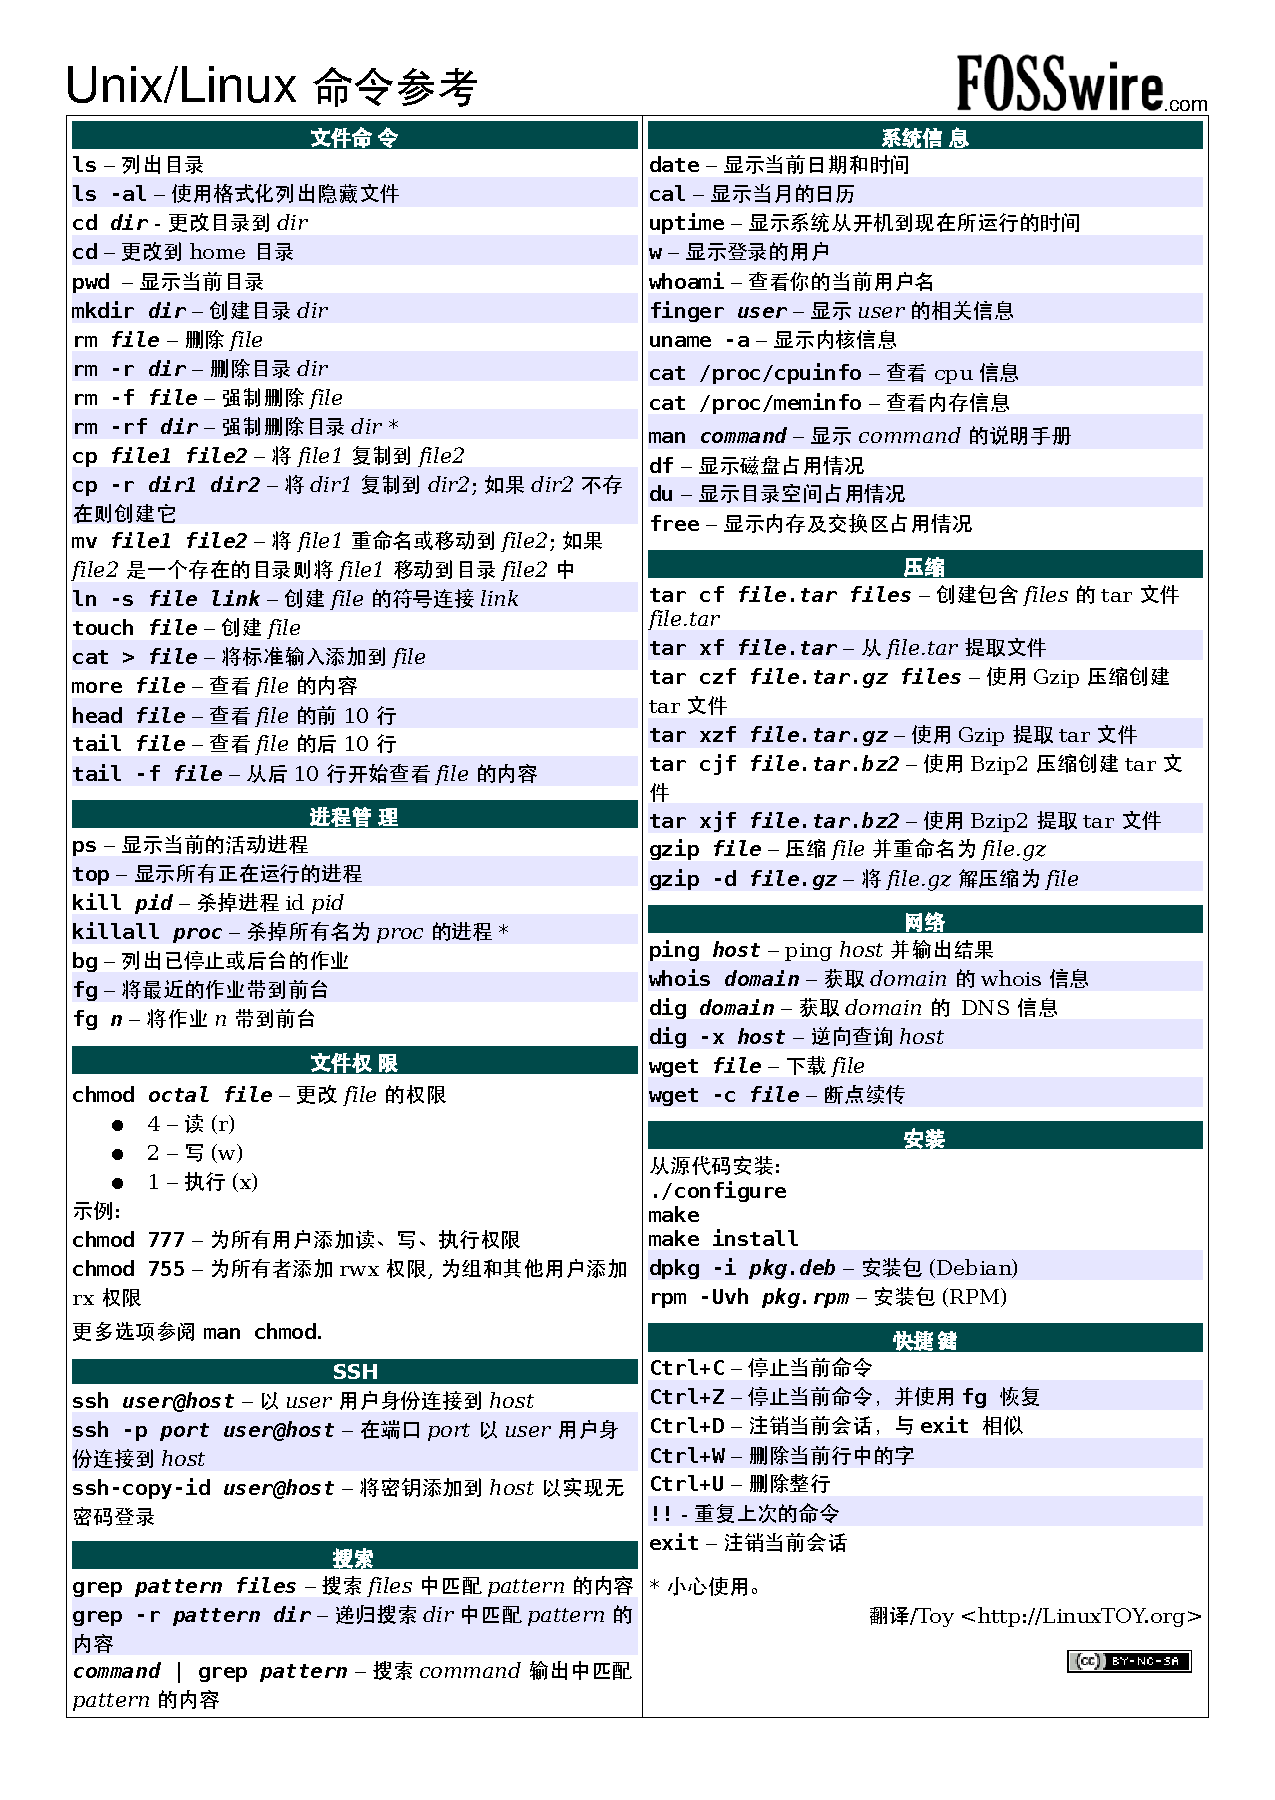
\includegraphics[scale=0.65]{unixref.pdf}
%%\end{figure}

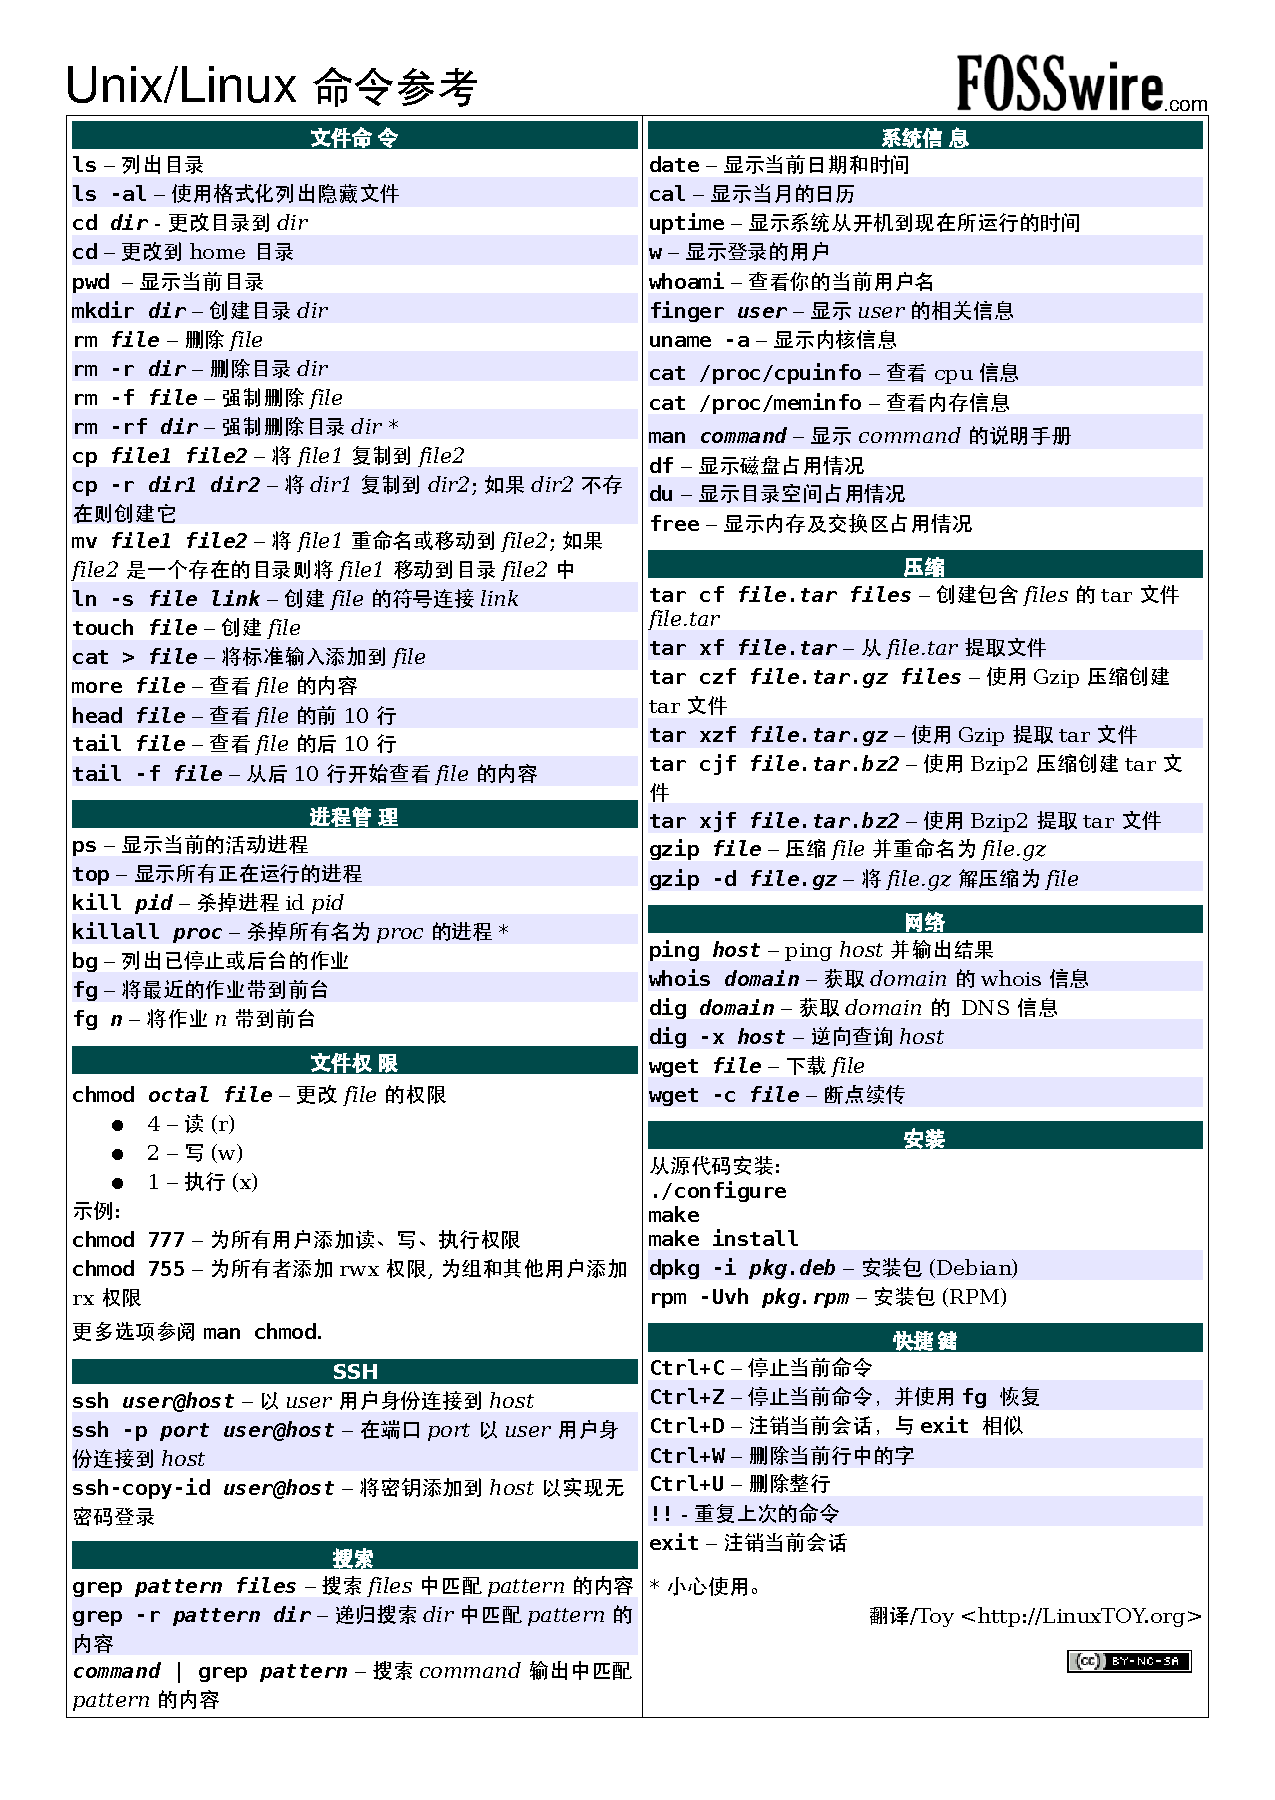
\includepdf[pages={1}]{unixref.pdf}

\chapter{Mozilla Firefox备忘表}

\vspace{-45pt}

\begin{figure}[!ht]
\centering
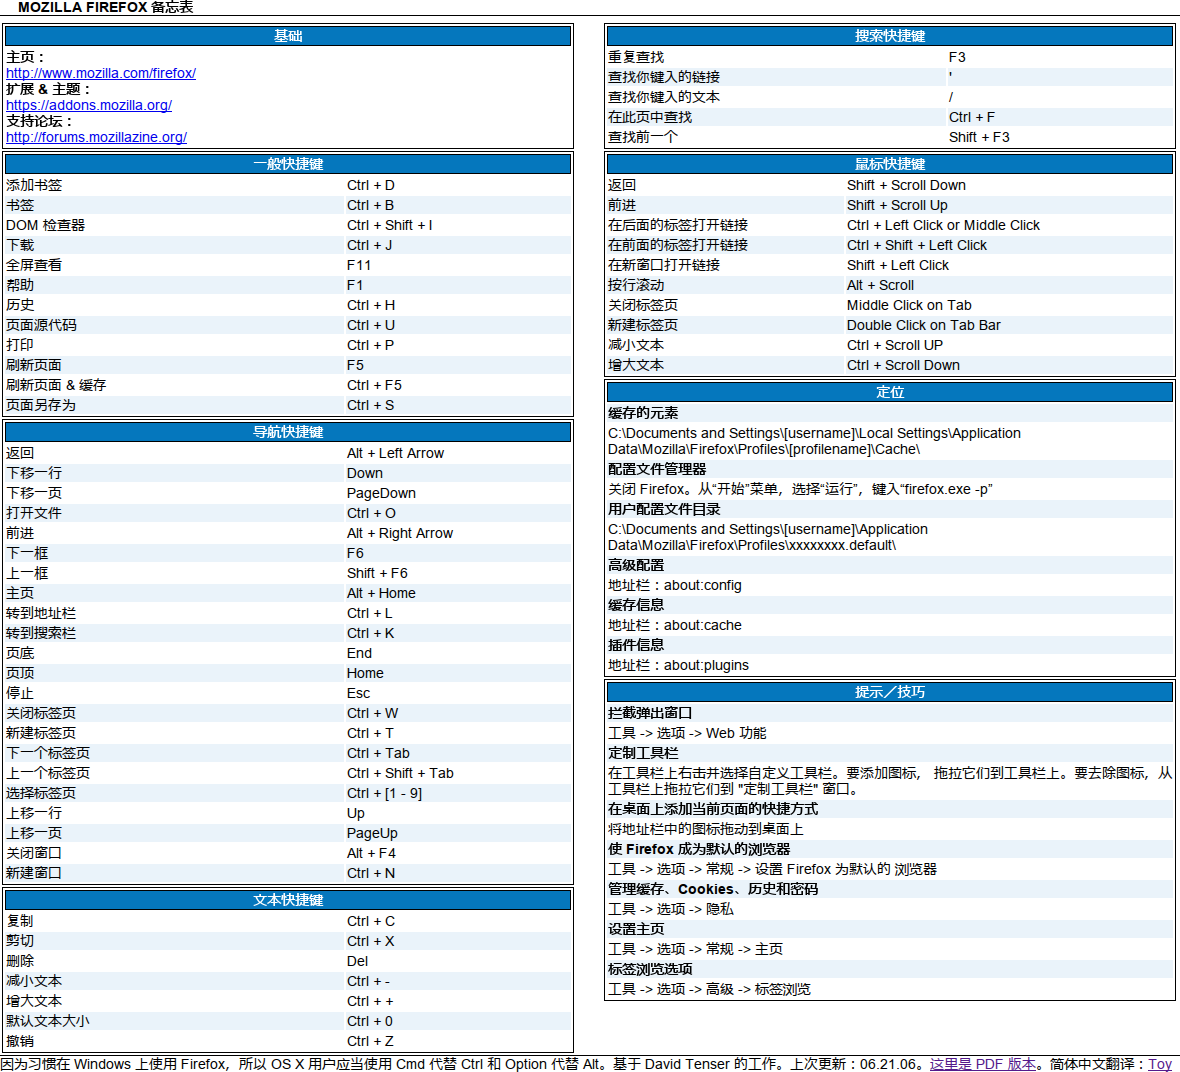
\includegraphics[scale=0.38]{firefoxcheatsheet.png}
\end{figure}

\clearpage

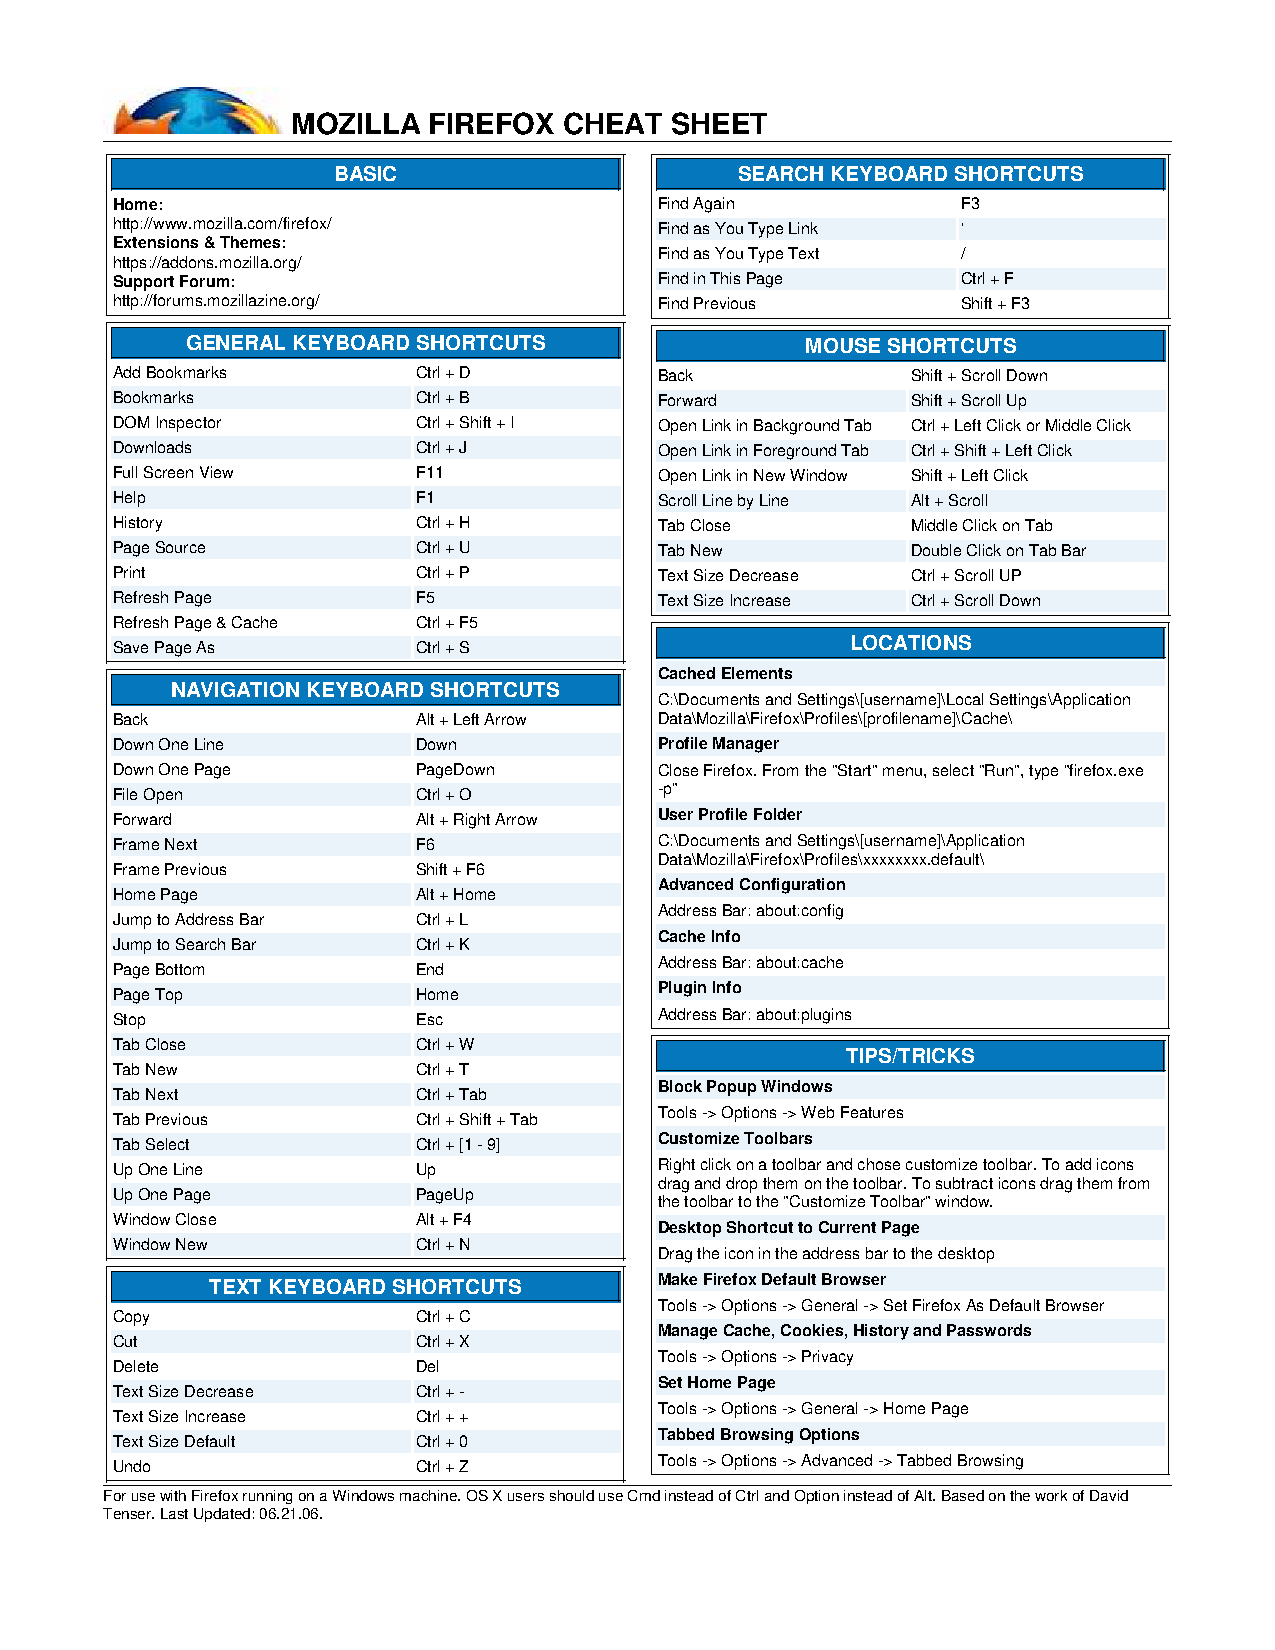
\includepdf[pages={1}]{firefoxcheatsheet.pdf}

\chapter{WordPress编辑快捷键速查表}


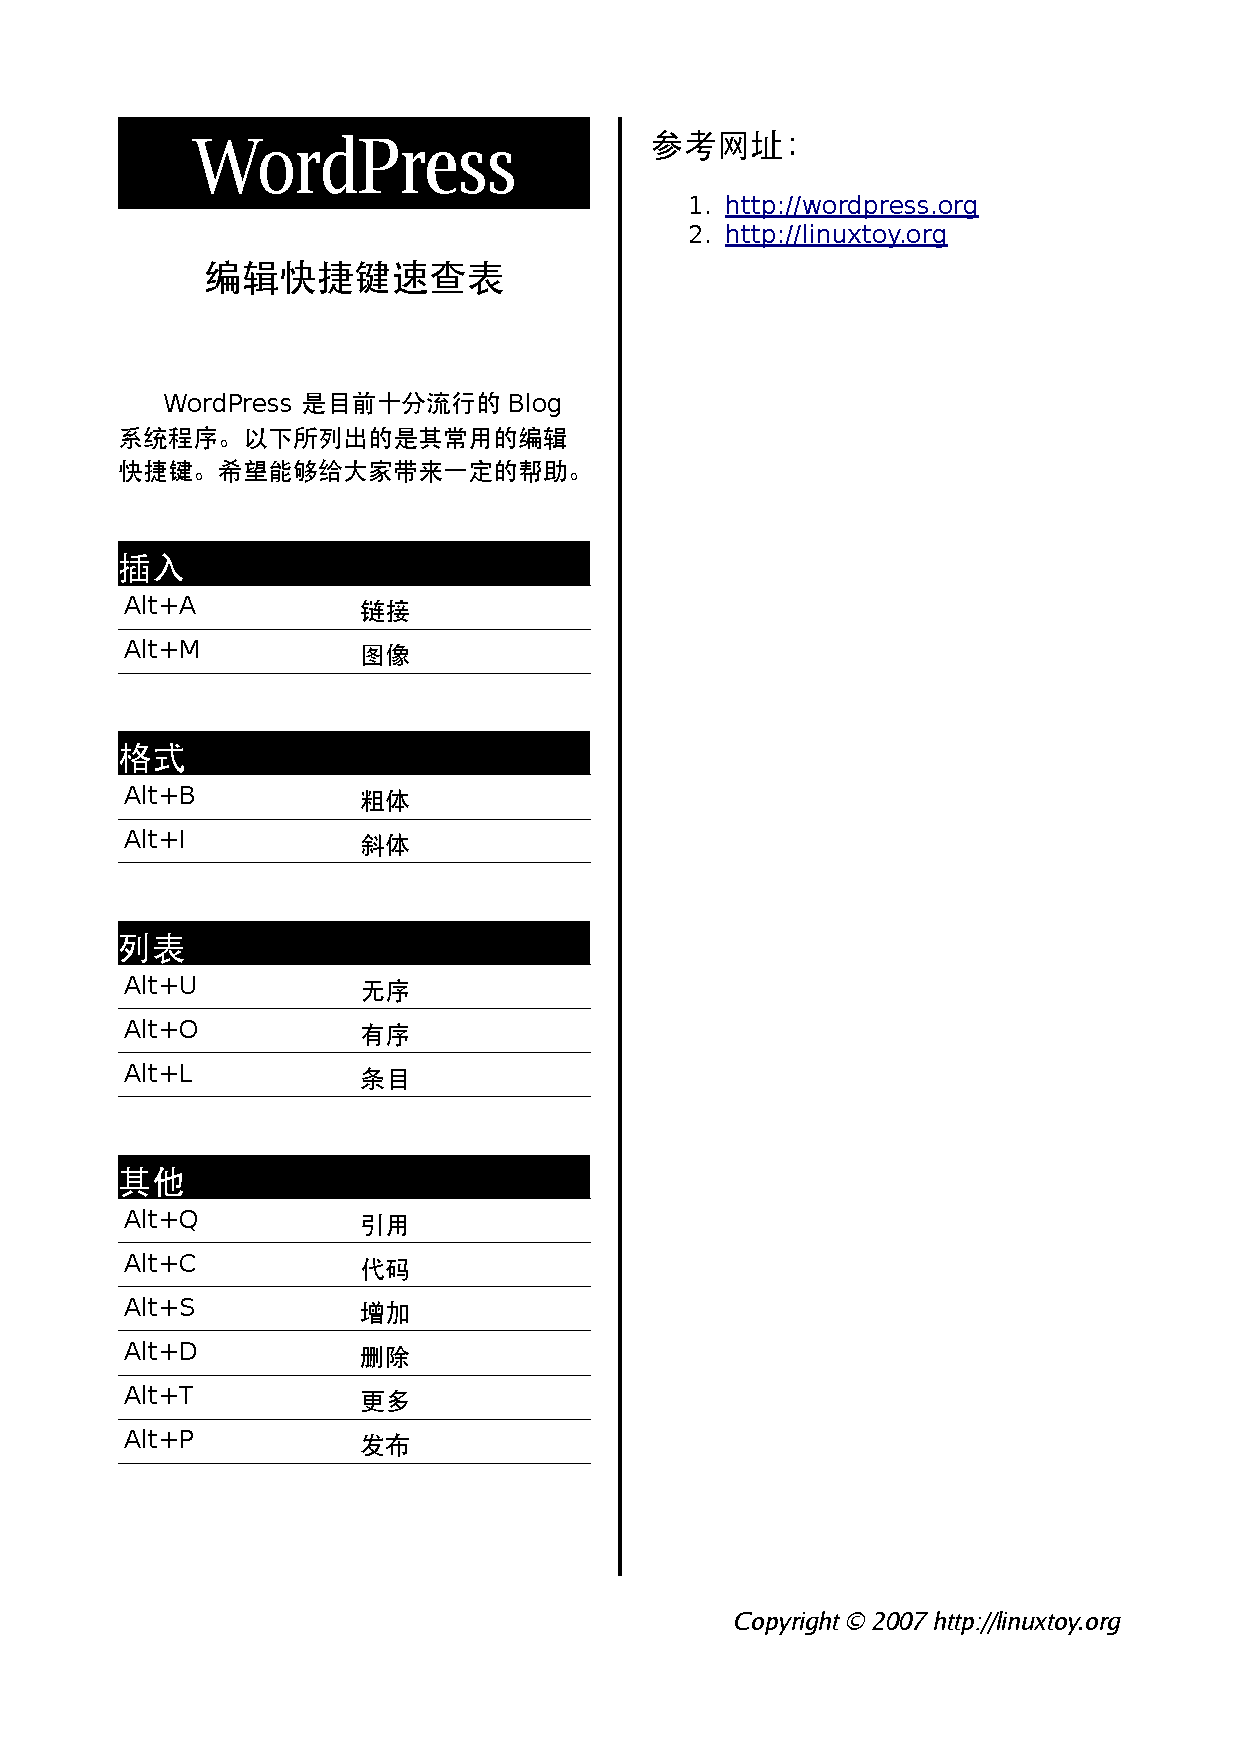
\includepdf[pages={1}]{wp-shortcuts.pdf}

\chapter{git cheat sheet}

\vspace{-50pt}

\begin{figure}[!ht]
\centering
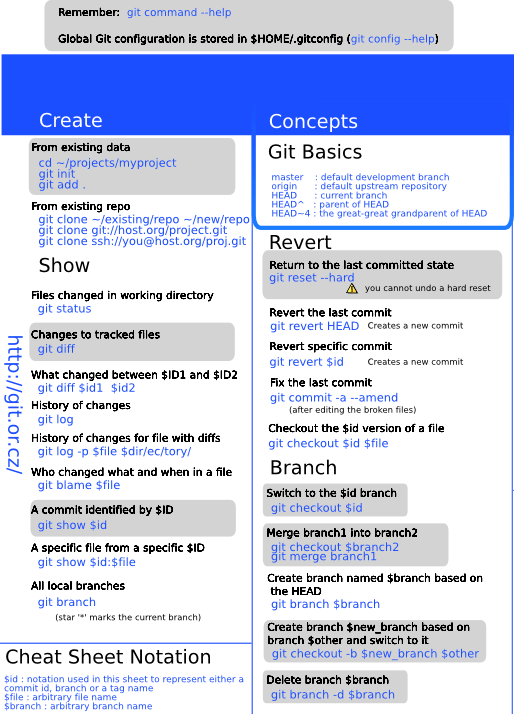
\includegraphics[scale=0.6]{git_cheat_sheet1.png}
\end{figure}

\clearpage


\begin{figure}[!ht]
\centering
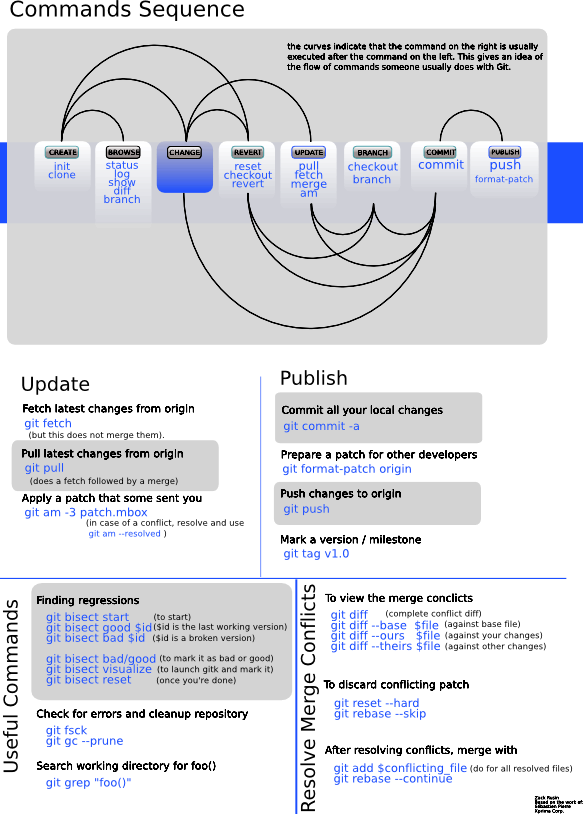
\includegraphics[scale=0.7]{git_cheat_sheet2.png}
\end{figure}

\chapter{究竟是喜欢一个人本身,还是喜欢一种预期}

出处:网络(豆瓣)\cite{love}


\begin{center}
原名:别向这个操蛋的世界投降\\ 作者:陈轩 
\end{center}

我妈常常喜欢念叨:人家又不喜欢你,你干嘛还要去喜欢人家。以前我一直想不出什么话反驳,只好简单粗暴地回应:一边去,你一老娘儿们你懂什么你。

我见过很多人,换男女朋友比换内裤还勤快的那种自不必说,还有像我们宿舍的闷骚青年,追女生,人家不睬他,他郁闷一阵子,提枪掉马就直奔下一目标而去了。我在旁边看的目瞪口呆。你要问他,他保准振振有词:人家又不屌我,我喜欢她有什么用。是的,有什么用。然后还会反过头来劝我:没用的,我跟你说$\cdots\cdots$这仿佛是如此的天经地义,如此的不证自明。 

昨天,我仔细地想了想,终于想通了这个问题。其中的关键就在于,你究竟是喜欢一个人本身,还是喜欢一种预期,一种前景,喜欢一种未来对方有可能和你上床睡觉结婚生子的可能性? 

这个年龄很多人都急吼吼地寻找另一半抱团取暖。要我说,其中有多少是真的喜欢对方本身,这很难说。我这么说可能一来打击面太广,二来没有调查取证,所以显得不那么令人信服。其实这很好判断,那就是扪心自问:换一个人行不行? 

这样多少有点神经质。对大多数人来说,并不存在一个绝对不可替代的the one。否则的话,这个世界会麻烦许多。小的时候,小到我才第一次思考爱情这回事的时候,我就对一个问题百思不得其解:你喜欢一个人,而这个人在茫茫人海中又恰巧喜欢你,这是多么大的一个巧合啊!而幼小的我放眼望去,这个世界上充斥着不可胜数的一对对巧合。 

要解释这样一件事,只能说明,在大多数人眼里,另一半绝不是不可替代的。而每一个个体的特质,很大程度上是相异的。换句话说,要追溯这种可替代性的载体,那可能就是每个个体作为伴侣所能为对方提供的“服务”了。 

比如说,深夜陪你聊天,闲暇陪你娱乐,工作学习相互鼓励,人情冷暖相互慰藉,生理需要相互解决。然后买房结婚,构筑家庭,生儿育女,传宗接代。老了之后相互扶持,终了一生。这些都只是些伴侣给你带来的效用而已。这个过程中,肯定会产生感情,不过这个感情的基础来自于这些过程当中一点一滴的积累,而不是来自于对方本身。换句话说,换一个人,你照样可以和他(她)积累起深厚的感情。而关键就看谁最开始和你开启这段旅程。 

所以,少不更事的时候,我们总以为只有某个特定的对象才能给我们带来这一切,只有他们才能给我们幸福感。而后长大了我们知道并不是这么回事。“好女人多的是的,何必呢。”我无数次地听见这句话。这就是所谓的成熟吧。 

这一切,也很美好。但这不是我想象中的爱情。 

就像我那个倔强的困惑,如果不存在将就凑合的心理考量,如果每个人都是固执的完美主义者,那么怎么可能你喜欢的人也正好喜欢你呢?但是,一旦喜欢,那便是雷打不动的定格。爱情所投射的对象本身基本不会产生多少重大的变化,除非她人品突变,性格突变,样貌突变,而这一切绝对是小概率事件。爱情对象在那,那么爱情本身便随之恒定。她不喜欢我,那么我也就不喜欢她了,这作何道理?我喜欢的是她这个人,而不是“她可能喜欢我”“我们可以像情侣一样生活”这种期盼。 

所以真正着眼于对象本身的爱情——我不敢说这是真正的爱情,但这是我理解的爱情——是这样的:她不认识我,我会喜欢她;我们点头相交,我会喜欢她;她拒绝我,我会喜欢她;她反复拒绝我,我还是喜欢她;她不回我信,不听我电话,不回我短信,我还是喜欢她;她和别的男人谈恋爱,我还是喜欢她;她和别的男人上床,我还是喜欢她;她和别的男人结婚,我还是喜欢她;她死了,我还是喜欢她。 

因为我喜欢的是她本人,她本人不变,感情就不会也没有理由变。这一切都不会随着她对我的态度,她自身的选择而变化。 

但是,这有什么用呢? 

“我想学哲学,我想学艺术。”“学这些有什么用呢,能当饭吃吗?” 

“我就是喜欢她”“她又不喜欢你,有什么用呢?” 

“这个社会为什么这么不公平?”“这个社会就这样,你说这些又有什么用呢?” 

是的,有什么用呢。我们每当面临内心的召唤的时候,这个问句都会鬼魅般如影随形。有时甚至不用父母亲友耳提面命,我们自己就习惯性地自问自责:有什么用呢?有什么用呢? 

那要是追问到底,我们生于世间,百年来往,又有什么用呢? 

如果生命是有意义的,那么我们内心的召唤就是有意义的。午夜梦回想到她时那满心酸楚难言的悸动,铺开信纸秉笔夜书时那字斟句酌的计较,经年再见面对佳人时那喷薄欲出的情意,这一切都是爱情原本的意义所在,这一切都是生命本身赋予的。 

这有什么用?这本身就是最大的意义。 

我们年轻时那些美丽的梦,它们往往敌不过这坚硬的世界,我们要将就,我们要放弃,我们要隐忍。比如爱情,谁年少时没有些洁白的向往。但我们敌不过现实的无奈,父母的唠叨,亲朋的压力,甚至敌不过我们自己本身内心的虚弱和不耐烦。然后我们就将其掩埋,扭头它寻,只有等到回首前尘时才泪满衣襟。 

我知道,很多人笑我幼稚。就连身边很好的朋友也常常对我说:“我保证,XX年之后你就不这样想了。”当然了,他们一再看着我过了XX年,还是一如既往地这么幼稚。这算幼稚吗?我只是觉得大家的理解不同罢了。 

当然,我并不是说我不会放弃。“也许有一天我会放弃,但是我绝不会像那些自以为看透了的人那样,等到将来自己的儿孙后辈面临这种类似的境遇的时候,傻逼哄哄地嘲讽他们,说一些“别犯傻了,爱情这东西,就是$\cdots\cdots$”之类的屁话。我会对他说,儿子,老爸当年也这样过,但是老爸比较没种,没有坚持到底,就向这个急躁的世界缴械投降了。希望你比老爸有出息。去吧,坚持你自己的内心,老爸支持你。” 

是的,虽然自知终须一败,但请再多坚持一会,别向这个操蛋的世界投降。


出处:网络

\bibliographystyle{plainnat}
\bibliography{gk}
\clearpage



\chapter{世上最伟大的十个公式}

来源:网络

英国科学期刊《物理世界》曾让读者投票评选了“最伟大的公式”,最终榜上有名的十个公式既有无人不知的$1+1=2$,又有著名的$E=mc^2$;既有简单的圆周公式,又有复杂的欧拉公式$\cdots\cdots$

从什么时候起我们开始厌恶数学?这些东西原本如此美丽,如此精妙。这个地球上有多少伟大的智慧曾耗尽一生,才最终写下一个等号。

每当你解不开方程的时候,不妨换一个角度想,暂且放下对理科的厌恶和对考试的痛恨,因为你正在见证的,是科学的美丽与人类的尊严。

No.$10\quad$圆的周长公式($The\ Length\ of\ the\ Circumference\ of\ a\ Circle$)$$c=2\pi r$$

目前,人类已经能得到圆周率的$2061$亿位精度。现代科技领域使用的圆周率值,有十几位已经足够了。

如果用$35$位精度的圆周率值来计算一个能把太阳系包起来的一个圆的周长,误差还不到质子直径的百万分之一。现在的人计算圆周率,多数是为了验证计算机的计算能力,还有就是为了兴趣。

No.$9\quad$傅立叶变换($The\ Fourier\ Transform$)$$\hat{f}(\xi):=\displaystyle\int_{-\infty}^{+\infty} f(x)e^{-2\pi ix\xi}dx$$

这个挺专业的,一般人完全不明白。这里不多作解释,简要地说没有这个式子没有今天的电子计算机,所以你能在这里上网要感谢这个完全看不懂的式子。

另外傅立叶虽然姓傅,但是法国人。

No.$8\quad$德布罗意方程组($The\ de\ Broglie\ Relations$)$$p=\hbar k$$ $$E=\hbar w $$

物理学中光学的很多概念跟它是远亲。简要地说德布罗意觉得电子不仅是一个粒子,也是一种波,它还有“波长”,于是就有了这个物质波方程,表达了波长、能量等等之间的关系,同时他获得了1929年诺贝尔物理学奖。

No.$7\quad$ $1+1=2$

这个公式不需要名称,不需要翻译,不需要解释。

No.$6\quad$薛定谔方程($The\ Schrdinger\ Equation$)$$\hbar\displaystyle\frac{\displaystyle\partial}{\displaystyle\partial t}\Psi (r,t)=\hat{H}\Psi(r,t)$$

也是一般人完全不明白的,因此摘录官方评价:“薛定谔方程是世界原子物理学文献中应用最广泛、影响最大的公式。”由于对量子力学的杰出贡献,薛定谔获得$1933$年诺贝尔物理奖。

另外薛定谔虽然姓薛,但是奥地利人。

No.$5\quad$质能方程($Mass–energy\  Equivalence$)$$E_0=mc^2$$

好像从来没有一个科学界的公式有如此广泛的意义。在物理学“奇迹年”——$1905$年,由一个叫做爱因斯坦的年轻人提出,同年他还发表了《论动体的电动力学》——俗称狭义相对论。

这个公式告诉我们,爱因斯坦是牛逼的,能量和质量是可以互换的,副产品就是——原子弹。

No.$4\quad$勾股定理/毕达哥拉斯定理($Pythagorean\ Theorem$)$$a^2+b^2=c^2$$

No.$3\quad$牛顿第二定律($Newton's\  Second\  Law\  of\  Motion$)$$F=ma$$

有史以来最伟大的没有之一的科学家在有史以来最伟大没有之一的科学巨作《自然哲学的数学原理》当中的被认为是经典物理学中最伟大的没有之一的核心定律,动力的所有基本方程都可由它通过微积分推导出来。

No.$2\quad$欧拉公式($Euler's\  Identity$)$$e^{i\pi}=1$$

这个公式是上帝写的么?到了最后几名,创造者个个是神人。欧拉是历史上最多产的数学家,也是各领域(包含数学的所有分支及力学、光学、音响学、水利、天文、化 学、医药等)最多著作的学者,数学史上称十八世纪为“欧拉时代”。

欧拉出生于瑞士,$31$岁丧失了右眼的视力,$59$岁双眼失明,但他性格乐观,有惊人的记忆力及集中力。他一生谦逊,很少用自己的名字给他发现的东西命名,不过还是命名了一个最重要的一个常数——$e$。

关于$e$,以前有一个笑话说:在一家精神病院里,有个病患整天对着别人说,“我微分你、我微分你。”也不知为什么,这些病患都有一点简单的微积分概念,总以为有一天自己会像一般多项式函数般,被微分到变成零而消失,因此对他避之不及,然而某天他却遇上了一个不为所动的人,他很意外,而这个人淡淡地对他说,“我是$e$的$x$次方。”

这个公式的巧妙之处在于,它没有任何多余的内容,将数学中最基本的$e$、$i$、$\pi$放在了同一个式子中,同时加入了数学也是哲学中最重要的$0$和$1$,再以简单的加号相连。

高斯曾经说:“一个人第一次看到这个公式而不感到它的魅力,他不可能成为数学家。”

No.$1\quad$麦克斯韦方程组($The\  Maxwell's\  Equations$)

积分形式:$$\displaystyle\oint\nolimits_{S}D\cdot dA=Q_{f,S}$$
$$\displaystyle\oint\nolimits_{S}B\cdot dA=0$$
$$\displaystyle\oint\nolimits_{\displaystyle\partial S}E\cdot dl=-\displaystyle\frac{\displaystyle\partial \Phi_{B,S}}{\displaystyle\partial t}$$
$$\displaystyle\oint\nolimits_{\displaystyle\partial S}H\cdot dl=I_{f,S}+\displaystyle\frac{\displaystyle\partial \Phi_{D,S}}{\displaystyle\partial t}$$

微分形式:$$\nabla \cdot D=\rho_{f}$$
$$\nabla \cdot B=0$$
$$\nabla \times E=-\displaystyle\frac{\displaystyle\partial B}{\displaystyle\partial t}$$
$$\nabla \times H=J_f+\displaystyle\frac{\displaystyle\partial D}{\displaystyle\partial t}$$

任何一个能把这几个公式看懂的人,一定会感到背后有凉风——如果没有上帝,怎么解释如此完美的方程?

这组公式融合了电的高斯定律、磁的高斯定律、法拉第定律以及安培定律。比较谦虚的评价是:“一般地,宇宙间任何的电磁现象,皆可由此方程组解释。”到后来麦克斯韦仅靠纸笔演算,就从这组公式预言了电磁波的存在。

我们不是总喜欢编一些故事,比如爱因斯坦小时候因为某一刺激从而走上了发奋学习、报效祖国的道路么?事实上,这个刺激就是你看到的这个方程组。

也正是因为这个方程组完美统一了整个电磁场,让爱因斯坦始终想要以同样的方式统一引力场,并将宏观与微观的两种力放在同一组式子中,即著名的“大一统理论”。

爱因斯坦直到去世都没有走出这个隧道,而如果一旦走出去,我们将会在隧道另一头看到上帝本人。

来源:网络


\chapter{提问的智慧}

\begin{center}
艾瑞克.史蒂文.雷蒙德(Eric Steven Raymond)\\
\href{http://www.catb.org/~esr/}{Thyrsus Enterprises}\\
\href{esr@thyrsus.com}{esr@thyrsus.com}\\
瑞克.莫恩(Rick Moen)\\
\href{respond-auto@linuxmafia.com}{respond-auto@linuxmafia.com}\\
\vspace{20pt}
版权©2001, 2006 Eric S. Raymond, Rick Moen\\
原文:\href{http://www.catb.org/~esr/faqs/smart-questions.html}{How To Ask Questions The Smart Way}\\
翻译\cite{smart_question}:王刚~\href{yafrank@126.com}{yafrank@126.com}\\
时间:2013年10月26日\\
\end{center}





\section{译文}

如果你想复制、镜像、翻译或引用本文,请参阅\href{http://www.catb.org/~esr/copying.html}{复制协议}。




\section{弃权申明}


许多项目的网站在如何取得帮助的部分链接了本文,这没有关系,也正是我们想要的。但如果你是该项目生成此链接的网管,请在链接附近显著位置注明:我们不提供该项目的服务支持!

我们已经领教了没有此说明带来的痛苦,我们将不停地被一些白痴纠缠,他们认为既然我们发布了本文,那么我们就有责任解决世上所有的技术问题。

如果你是因为需要帮助正在阅读本文,然后就带着可以直接从作者那取得帮助的印象离开,那么你就不幸成了我们所说的白痴之一。 别向我们提问,我们不会理睬的。 我们只是在这教你如何从那些真正懂得你软硬件问题的人那里取得帮助,但 99.9\% 的时间我们不会是那些人。除非你非常地 确定 本文的作者是你遇到问题方面的专家,请不要打搅,这样大家都更开心一点。






\section{引言}


在\href{http://www.catb.org/~esr/faqs/hacker-howto.html}{黑客}的世界里,你所提技术问题的解答很大程度上取决于你提问的方式与解决此问题的难度,本文将教你如何提问才更有可能得到满意的答复。

开源程序的应用已经很广,你通常可以从其他更有经验的用户而不是黑客那里得到解答。这是好事,他们一般对新手常有的毛病更容忍一点。然尔,使用我们推荐的方法,象对待黑客那样对待这些有经验的用户,通常能最有效地得到问题的解答。

第一件需要明白的事是黑客喜欢难题和激发思考的好问题。假如不是这样,我们也不会写本文了。如果你能提出一个有趣的问题让我们咀嚼玩味,我们会感激你。好问题是种激励与礼物,帮助我们发展认知,揭示没有注意或想到的问题。在黑客中,“好问题!” 是非常热烈而真挚的赞许。

此外,黑客还有遇到简单问题就表现出敌视或傲慢的名声。有时,我们看起来还对新手和愚蠢的家伙有条件反射式的无礼,但事情并不真是这样。

我们只是毫无歉意地敌视那些提问前不愿思考、不做自己家庭作业的人。这种人就象时间无底洞──他们只知道索取,不愿意付出,他们浪费了时间,这些时间本可用于其它更有趣的问题或更值得回答的人。我们将这种人叫做 “失败者(loser)” (由于历史原因,我们有时将“loser”拼写为“lusers” 。)

我们意识到许多人只是想使用我们写的软件,他们对学习技术细节没有兴趣。对大多数人而言,计算机只是种工具,是种达到目的的手段而已。他们有自己的生活并且有更要紧的事要做,我们承认这点,也从不指望每个人都对这些让我们着迷的技术问题感兴趣。不过,我们回答问题的风格是为了适应那些真正对此有兴趣并愿意主动参与解决问题的人,这一点不会变,也不该变。如果连这都变了,我们就会在自己能做得最好的事情上不再那么犀利。

我们(大多数)是自愿者, 从自己繁忙的生活中抽时间来回答问题,有时会力不从心。因此,我们会毫不留情地滤除问题,特别是那些看起来象是失败者提的,以便更有效地把回答问题的时间留给那些胜利者。

如果你认为这种态度令人反感、以施惠者自居或傲慢自大,请检查你的假设,我们并未要求你屈服──事实上,假如你做了该做的努力,我们中的大多数将非常乐意平等地与你交流,并欢迎你接纳我们的文化。试图去帮助那些不愿自救的人对我们简直没有效率。不懂没有关系,但愚蠢地做事不行。

所以,你不必在技术上很在行才能吸引我们的注意,但你 必须 表现出能引导你在行的姿态──机 敏、有想法、善于观察、乐于主动参与问题的解决。如果你做不到这些使你与众不同的事情,我们建议你付钱跟别人签商业服务合同,而不是要求黑客无偿帮助。

如果你决定向我们求助,你不会想成为一名失败者,你也不想被看成一个失败者。得到快速有效回答的最好方法是使提问者看起来象个聪明、自信和有想法的人,并且暗示只是碰巧在某一特别问题上需要帮助。

(欢迎对本文指正,可以将建议发至 \href{mailto:esr@thyrsus.com}{esr@thyrsus.com}或\href{mailto:esr@thyrsus.com}{respond-auto@linuxmafia.com}。 请注意,本文不想成为一般性的\href{http://www.ietf.org/rfc/rfc1855.txt}{网络礼仪}指南,我一般会拒绝那些与引出技术论坛中有用的回答不特别相关的建议。)




\section{提问前}


在通过电邮、新闻组或论坛提技术问题以前,做以下事情:

\begin{compactenum}
\item 尝试在你准备提问论坛的历史文档中搜索答案
\item 尝试搜索互联网以找到答案
\item 尝试阅读手册以找到答案
\item 尝试阅读“常见问题文档”(FAQ)以找到答案
\item 尝试自己检查或试验以找到答案
\item 尝试请教懂行的朋友以找到答案
\item 如果你是程序员,尝试阅读源代码以找到答案
\end{compactenum}



提问时,请先表明你已做了上述事情,这将有助于建立你不是寄生虫与浪费别人时间的印象。最好再表述你从中 学到的东西 ,我们喜欢回答那些表现出能从答案中学习的人。

运用某些策略,比如用谷歌(Google)搜索你遇到的各种错误提示(既搜索 谷歌论坛,也搜索网页), 这样很可能直接就找到了解决问题的文档或邮件列表线索。 即使没有结果,在邮件列表或新闻组寻求帮助时提一句“我在谷歌中搜过下列句子但没有找到什么有用的东西” 也是件好事,至少它表明了搜索引擎不能提供哪些帮助。将搜索关键词与你的问题及可能的解决方案联系起来,还有助于引导其他有类似问题的人。

别着急,不要指望几秒钟的谷歌搜索就能解决一个复杂的问题。读一下常见问题文档。在向专家提问之前,先向后靠靠放松一下,再思考一下问题。相信我们,他们能从你的提问看出你做了多少阅读与思考,如果你是有备而来,将更有可能得到解答。不要将所有问题一股脑抛出,只因你的第一次搜索没有结果(或者结果太多)。

认真地思考,准备好你的问题。轻率的提问只能得到轻率的回答,或者压根没有。在提问时,你越是表现出在此前做过思考与努力去解决自己的问题,你越有可能得到真正的帮助。

注意别提错问题。如果提问基于错误的假设,某黑客多半会一边想 “愚蠢的问题……”,一边按将错就错的答案回复你,并且希望这种只是得到你自己“问的问题”而非真正所需的解答,给你一个教训。

永远不要假设你 有资格 得到解答。你没有这种资格,毕竟你没有为此服务付费。如果你能够提出有内容、有趣和激励思考的问题──那种毫无疑问能够向社区贡献经验,而不仅仅是消极地要求从别人那获取知识的问题,你将“挣到”答案。

另一方面,表明你有能力也乐意参与问题的解决是个很好的开端。“有没有人能指个方向?”,我这还差点什么?”,“我应该查哪个网站?”,通常要比 “请给出我可以用的完整步骤”更容易得到回复,因为你表明了只要有人能指个方向,你就很乐意完成剩下的过程。




\section{提问时}


\subsection{仔细挑选论坛}

要对在哪提问留心,如果你做了下述事情,多半会被一笔勾销或被看成“失败者”:


\begin{compactenum}
\item 张贴与论坛主题无关的问题
\item 在面向高级技术问题的论坛上张贴肤浅的问题,或者反之。
\item 在太多不同的新闻组同时张贴
\item 给既非熟人也没有义务解决你问题的人发送你私人的电邮
\end{compactenum}



为保护通信的渠道不被无关的东西淹没,黑客会除掉那些没有找对地方的问题,你不会想让这种事落到自己头上的。

因此,第一步是找对论坛。谷歌和其它搜索引擎还是你的朋友,可以用它们搜索你遇到困难的软硬件问题最相关的项目网站。那里通常都有项目的常见问题(FAQ)、邮件列表及文档的链接。如果你的努力(包括 阅读 FAQ)都没有结果,这些邮件列表就是最后能取得帮助的地方。项目的网站也许还有报告臭虫的流程或链接,如果是这样,去看看。

向陌生的人或论坛发送邮件极有可能是在冒险。譬如,不要假设一个内容丰富的网页的作者想充当你的免费顾问,不要对你的问题是否会受到欢迎做太乐观的估计──如果你不确定,向别处发或者压根别发。

在选择论坛、新闻组或邮件列表时,别太相信名字,先看看 FAQ 或者许可书以明确你的问题是否切题。发贴前先翻翻已有的帖子,这样可以让你感受一下那里行事的方式。事实上,张贴前在新闻组或邮件列表的历史文档中搜索与你问题相关的关键词是个极好的主意,也许就找到答案了。即使没有,也能帮助你归纳出更好的问题。

别象机关枪似的一次性“扫射”所有的帮助渠道,这就象大喊大叫一样会令人不快,温柔地一个一个来。

弄懂主题!最典型的错误之一是在某种致立于跨平台可移植的语言、库或工具的论坛中提关于 Unix 或 Windows 操作系统程序接口的问题。如果你不明白为什么这是大错,最好在搞清楚概念前什么也别问。

一般来说,在仔细挑选的公共论坛中提问比在私有论坛中提同样的问题更容易得到有用的回答。有几个道理支持这点,一是看潜在的回复者有多少,二是看论坛的参与者有多少,黑客更愿回答能启发多数人的问题。

可以理解,老练的黑客和一些流行软件的作者正在承受过多的不当消息。就象那根最后压垮骆驼背的稻草一样,你的加入也有可能使情况走向极端──已经好几次了,一些流行软件的作者退出了对自己软件的支持,因为伴随而来的涌入其私人邮箱的垃圾邮件变得无法忍受。


\subsection{面向新手的论坛和互联网中继聊天(IRC)通常响应最快}

本地的用户组织或者你所用的 Linux 发行版也许正在宣传新手取得帮助的论坛或 IRC 通道(在一些非英语国家,新手论坛很可能还是邮件列表),这些地方是开始提问的好去处,特别是当你觉得遇到的也许只是相对简单或者很普通的问题时。经过宣传的 IRC 通道是公开邀请提问的地方,通常可以得到实时的回复。

事实上,如果出问题的程序来自某发行版(这很常见),最好先去该发行版的论坛或邮件列表中提问,再到程序本身的项目论坛或邮件列表,(否则)该项目的黑客可能仅仅回复“用 我们的 代码”。

在任何论坛发贴以前,先看看有没有搜索功能。如果有,就试着用问题的几个关键词搜索一下,也许就有帮助。如果在此之前你已做过全面的网页搜索(你应该这样去做),还是再搜索一下论坛,搜索引擎有可能没来得及索引此论坛的全部内容。

通过论坛或 IRC 通道提供项目的用户支持有增长的趋势,电子邮件交流则更多地为项目开发者保留。所以先在论坛或 IRC 中寻求与该项目相关的帮助。



\subsection{第二步,使用项目的邮件列表}

当某个项目存在开发者邮件列表时,要向列表而不是其中的个别成员提问,即使你确信他能最好地回答你的问题。查一查项目的文档和主页,找到项目的邮件列表并使用它。采用这种办法有几个很好的理由:


\begin{compactitem}
\item 向个别开发者提的问题(如果)足够好,也将对整个项目组有益。相反,如果你认为自己的问题对整个项目组来说太愚蠢,这也不能成为骚扰个别开发者的理由。
\item 向列表提问可以分散开发者的负担,个别开发者(尤其是项目领导)也许太忙以至于没法回答你的问题。
\item 大多数邮件列表都要存档,那些存档将被搜索引擎索引,如果你向列表提问并得到解答,将来其它人可以通过网页搜索找到你的问题和答案,也就不用再次发问了。
\item 如果某些问题经常被问到,开发者可以利用此信息改进文档或软件本身,以使其更清楚。如果只是私下提问,就没有人能看到最常见问题的完整场景。
\end{compactitem}

如果一个项目既有 “用户” 也有“开发者”(或 “黑客”)邮件列表或论坛,而你又不摆弄那些代码,向“用户”列表或论坛提问。不要假设自己会在开发者列表中受到欢迎,那些人多半会遭受你的噪音干扰。

然尔,如果你 确信 你的问题不一般,而且在“用户” 列表或论坛中几天都没有回复,可以试试“开发者”列表或论坛。建议你在张贴前最好先暗暗地观察几天,至少看看最近几天保存的帖子,以了解那的行事方式(事实上这是参与任何私有或半私有列表的好主意)

如果你找不到一个项目的邮件列表,而只能查到项目维护者的地址,只管向其发信。即便在这种情况下,也别假设(项目)邮件列表不存在。在你的电子邮件中陈述你已经试过但没有找到合适的邮件列表,也提及你不反对将自己的邮件转发给他人(许多人认为,即使没什么秘密,私人电子邮件也不应该被公开。通过允许将你的电子邮件转发他人,你给了相应人员处置你邮件的选择)。





\subsection{使用有意义且明确的主题}

在邮件列表、新闻组或论坛中,主题是你在五十个或更少的字以内吸引有资格专家注意的黄金机会,不要用诸如 “请帮我” (更别提大写的 “请帮我!!!!”,这种主题的消息会被条件反射式地删掉)之类的唠叨浪费机会。不要用你痛苦的深度来打动我们,相反,要在这点空间中使用超级简明扼要的问题描述。

使用主题的好惯例是“对象──偏差”(式的描述),许多技术支持组织就是这样做的。在“对象”部分指明是哪一个或哪一组东西有问题,在“偏差”部分则描述与期望的行为不一致的地方。

\textbf{愚蠢:}

救命啊!我的笔记本视频工作不正常!

\textbf{明智:}


X.org 6.8.1 扭曲鼠标光标,MV1005 型号的某显卡芯片组

\textbf{更明智:}



使用 MV1005 型号的某显卡芯片组在 X.org 6.8.1 的鼠标光标被扭曲

编写 “对象──偏差”式描述的过程有助于你组织对问题的细致思考。是什么被影响了?仅仅是鼠标光标或者还有其它图形?只在 X.org 中出现?或只是在其 6.8.1 版中?是针对某显卡芯片组?或者只是其中的 MV1005 型号?一个黑客只需描一眼就能够立即明白什么是你遇到的问题,什么是你自己的问题。

更一般地,想象一下在一个只显示主题的文档索引中查找。让你的主题更好地反映问题,可以使下一个搜索类似问题的人能够在文档中直接就找到答案的线索,而不用再次发贴提问。

如果你想在回复中提问,确保改变主题以表明你是在问一个问题,一个主题象 “Re: 测试” 或者 “Re: 新臭虫”的消息不太可能引起足够的注意。同时,将回复中与新主题不甚相关的引用内容尽量删除。

对于列表消息,不要直接点击回复(按钮)来开始一个全新的线索,这将限制你的观众。有些邮件阅读程序,比如 mutt,允许用户按线索排序并通过折叠线索来隐藏消息,这样做的人永远看不到你发的消息。

仅仅改变主题还不够。mutt 和其它一些邮件阅读程序还要检查邮件头主题以外的其它信息,以便为其指定线索,所以宁可发一个全新的邮件。

在论坛,因为消息与特定的线索紧密结合,并且通常在线索之外不可见,好的提问方式略有不同,通过回复提问并不要紧。不是所有论坛都允许在回复中出现分离的主题,而且这样做了基本上没有人会去看。不过,通过回复提问本身就是令人怀疑的做法,因为它们只会被正在查看该线索的人读到。所以,除非你 只想 在该线索当前活跃的人群中提问,还是另起炉灶比较好。




\subsection{使问题容易回复}


以“请向……回复”来结束问题多半会使你得不到回答。如果你觉得花几秒钟在邮件客户端设置一下回复地址都麻烦,我们也觉得花几秒钟考虑你的问题更麻烦。如果你的邮件客户端程序不支持这样做,换个好点的;如果是操作系统不支持所有这种邮件客户端程序,也换个好点的。

在论坛,要求通过电子邮件回复是完全无礼的,除非你确信回复的信息也许是敏感的(而且有人会为了某些未知的原因,只让你而不是整个论坛知道答案)。如果你只是想在有人回复线索时得到电子邮件提醒,可以要求论坛发送。几乎所有论坛都支持诸如“留意本线索”、“有回复发送邮件”等功能。



\subsection{用清晰、语法、拼写正确的语句书写}

经验告诉我们,粗心与草率的作者通常也粗心与草率地思考和编程(我敢打赌)。为这些粗心与草率的思考者回答问题没有什么好处,我们宁可将时间花在其它地方。

清楚、良好地表达你的问题非常重要。如果你觉得这样做麻烦,我们也觉得注意(你的问题)麻烦。花点额外的精力斟酌一下字句,用不着太僵硬与正式──事实上,黑客文化很看重能准确地使用非正式、俚语和幽默的语句。但它 必须 很准确,而且有迹象表明你是在思考和关注问题。

正确地拼写、使用标点和大小写,不要将“its”混淆为“it's”,“loose”搞成“lose”或者将“discrete”弄成 “discreet”。不要全部用大写,这会被视为无礼的大声嚷嚷 (全部小写也好不到哪去,因为不易阅读。Alan Cox [注:著名黑客,Linux 内核的重要参与者] 也许可以这样做,但你不行。)

一般而言,如果你写得象个半文盲似的傻子,多半得不到理睬。也不要使用即时通讯中的简写,如将“you”简化为“u”会使你看起来象一个为了节约二次击键的半文盲式的傻子。更糟的是,如果象个小孩似地鬼画桃符那绝对是在找死,可以肯定没人会理你(或者最多是给你一大堆指责与挖苦)。

如果在非母语论坛提问,你的拼写与语法错误会得到有限的宽容,但懒惰完全不会被容忍(是的,我们通常看得出其中的差别)。同时,除非你知道回复者使用的语言,请使用英语书写。繁忙的黑客一般会直接删除用他们看不懂语言写的消息。在互联网上英语是工作语言,用英语书写可以将你的问题不被阅读就被直接删除的可能性降到最低。

如果你用英语书写但它是你的第二语言,最好提醒潜在的回复者语言上可能的困难以便绕过这个问题,比如:

\begin{compactitem}
\item 英语不是我的母语,请谅解拼写错误。
\item 如果您使用某某语言,请电邮/私聊我,也许我需要您的协助翻译我的问题。
\item 对于这个技术术语本身我很熟悉,但对于它的一些俚语或习惯表达方式就不太明白了。
\item 我已经同时用某某语及英语提问,如果您使用两者之一回复,我很乐意翻译。
\end{compactitem}







\subsection{使用易于读取且标准的文件格式发送问题}

如果你人为地将问题搞得难以阅读,它多半会被忽略,人们更愿读易懂的问题,所以:

\begin{compactitem}
\item 使用纯文本而不是 HTML(超文本标注语言)( 关闭HTML 并不难)
\item 使用 MIME(多用途互联网邮件扩展)附件通常没有问题,前提是真正有内容(譬如附带的源文件或补丁),而不仅仅是邮件客户端程序生成的模板(譬如只是消息内容的拷贝)。
\item 不要发送整段只是单行句子但多次折回的邮件(这使得回复部分内容非常困难)。设想你的读者是在80个字符宽的文本终端阅读邮件,设置你的行折回点小于 80 列。
\item 但是,也 不要 用任何固定列折回数据(譬如日志文件拷贝或会话记录)。数据应该原样包含,使回复者确信他们看到的是与你看到的一样的东西。
\item 在英语论坛中,不要使用'Quoted-Printable' MIME 编码发送消息。这种编码对于张贴非 ASCII 语言可能是必须的,但很多邮件程序并不支持。当它们分断时,那些文本中四处散布的 “=20”符号既难看也分散注意力,甚至有可能破坏内容的语意。
\item 永远不要 指望黑客们阅读使用封闭的专用格式编写的文档,诸如微软公司的 Word 或 Excel 文件等。大多数黑客对此的反应就象有人将还在冒热气的猪粪倒在你门口时你的反应一样。即使他们能够处理,也很厌恶这么做。
\item 如果你从使用视窗的电脑发送电子邮件,关闭问题颇多的微软“聪明引用”功能(在“工具” -> “自动纠正选项”的“输入时自动格式化”下去掉聪明引用的选框),以免在你的邮件中到处散布垃圾字符。
\item 在论坛,勿滥用“表情符号”和“HTML”功能(当它们提供时)。一两个表情符号通常没有问题,但花哨的彩色文本倾向于使人认为你是个无能之辈。过滥地使用表情符号、色彩和字体会使你看来象个傻笑的小姑娘。这通常不是个好主意,除非你只是对性而不是有用的回复更有兴趣。
\end{compactitem}

如果你使用图形用户界面的邮件客户端程序(如网景公司的 Messenger、微软公司的 Outlook 或者其它类似的),注意它们的缺省配置不一定满足这些要求。大多数这类程序有基于菜单的“查看源码”命令,用它来检查发送文件夹中的消息,以确保发送的是没有多余杂质的纯文本文件。






\subsection{描述问题应准确且有内容}

\begin{compactitem}
\item 仔细、清楚地描述问题的症状
\item 描述问题发生的环境(主机、操作系统、应用程序,任何相关的),提供销售商的发行版和版本号(如:“Fedora Core 7”、“Slackware 9.1”等)
\item 描述提问前做过的研究及其理解。
\item 描述提问前为确定问题而采取的诊断步骤。
\item 描述最近对计算机或软件配置的任何相关改变。
\item 如果可能,提供在可控环境下重现问题的方法。
\end{compactitem}

尽最大努力预测黑客会提到的问题,并提前备好答案。

如果你认为是代码有问题,向黑客提供在可控环境下重现问题的方法尤其重要。当你这么做时,得到有用且及时回复的可能性将大大增加。

西蒙.泰瑟姆(Simon Tatham)写过一篇\href{http://www.chiark.greenend.org.uk/~sgtatham/bugs.html}{如何有效报告臭虫}的文章,我强烈推荐各位阅读。



\subsection{量不在多,精炼则灵}
\label{not_much}

你应该(写得)精炼且有内容,简单地将一大堆代码或数据罗列在求助消息中达不到目的。如果你有一个很大且复杂的测试样例让程序崩溃,尝试将其裁剪得越小越好。

至少有三个理由支持这点。第一,让别人看到你在努力简化问题使你更有可能得到回复。第二,简化问题使你更有可能得到 有用的 回复。第三,在提纯臭虫报告的过程中,你可能自己就找到了解决办法或权宜之计。


\subsection{别急于宣称找到臭虫}


当你在一个软件中遇到问题,除非你 非常、非常 的有根据,不要动辄声称找到了臭虫。提示:除非你能提供解决问题的源代码补丁,或者对前一版本的回归测试表现出不正确的行为,否则你都多半不够完全确信。对于网页和文档也如此,如果你(声称)发现了文档的“臭虫”,你应该能提供相应位置的替代文本。

记住,还有许多其它用户并未经历你遇到的问题,否则你在阅读文档或搜索网页时就应该发现了(你在报怨前已经做了这些,是吧 ?)。这也意味着很有可能是你弄错了而不是软件本身有问题。

编写软件的人总是非常辛苦地使它尽可能完美。如果你声称找到了臭虫,也就置疑了他们的能力,即使你是对的,也有可能会使其中的部分人感到不快。(此外,)在主题中嚷嚷“臭虫”也是特别不老练的。

提问时,即使你私下非常确信已经发现一个真正的臭虫,最好写得象是 你 做错了什么。如果真的有臭虫,你会在回复中看到这点。这样做的话,如果真有虫子,维护者就会向你道歉,这总比你弄砸了然后欠别人一个道歉要强。





\subsection{低声下气代替不了做自己的家庭作业}


有些人明白他们不应该粗鲁或傲慢地行事并要求得到答复,但他们退到相反的低声下气的极端:“我知道我只是个可怜的新丁,一个失败者,但……”。这既使人困扰,也没有用,当伴随着对实际问题含糊的描述时还特别令人反感。

别用低级灵长类动物的办法浪费你我的时间,相反,尽可能清楚地描述背景情况和你的问题,这比低声下气更好地摆正了你的位置。

有时,论坛设有单独的初学者提问版面,如果你真的认为遇到了肤浅的问题,到那去就是了,但一样别低声下气。




\subsection{描述问题症状而不是猜测}

告诉黑客是什么导致了问题是没用的(如果你的诊断理论是了不起的东西,你还会向别人咨询求助吗?)。所以,确保只是告诉他们问题的原始症状,而不是你的解释和理论,让他们来解释和诊断。如果你认为陈述自己的猜测很重要,应清楚地说明这只是你的猜测并描述为什么它们不起作用。

\textbf{愚蠢:}

我在编译内核时接连遇到 SIG11 错误,怀疑主板上的某根电路丝断了,找到它们的最好办法是什么?

\textbf{明智:}

我组装的电脑(K6/233 CPU、FIC-PA2007 主板[威盛 Apollo VP2 芯片组]、Corsair PC133 SDRAM 256Mb 内存)最近在开机 20 分钟左右、做内核编译时频繁地报 SIG11 错,但在头 20 分钟内从不出问题。重启动不会复位时钟,但整夜关机会。更换所有内存未解决问题,相关的典型编译会话日志附后。

由于以上这点许多人似乎难以掌握,这里有句话可以提醒你:“所有的诊断专家都来自密苏里州”。美国国务院的官方座右铭则是“让我看看”(出自国会议员威勒德.D.范迪弗[Willard D. Vandiver]在1899年时的讲话:“我来自一个出产玉米、棉花、牛蒡和民主党人的国家,滔滔雄辩既不能说服我,也不会让我满意。我来自密苏里州,你必须让我看看。”)针对诊断者而言,这并不是怀疑,而只是一种真实而有用的需求,以便让他们看到与你看到的原始证据尽可能一致的东西,而不是你的猜测与总结。(所以,)让我们看看。




\subsection{按时间先后罗列问题症状}

刚出问题之前发生的事情通常包含有解决问题最有效的线索。所以,记录中应准确地描述你、电脑和软件在崩溃前都做了什么。在命令行处理的情况下,有会话日志(如运行脚本工具生成的)并引用相关的若干(如20)行记录会非常有帮助。

如果崩溃的程序有诊断选项(如-v详述开关),试着选择这些能在记录中增加排错信息的选项。记住,“多”不等于“好”。试着选取适当的排错级别以便提供有用的信息而不是将阅读者淹没在垃圾中。

如果你的记录很长(如超过四段),在开头简述问题随后按时间先后罗列详细过程也许更有用。这样,黑客在读你的记录时就知道该注意哪些内容了。





\subsection{描述目标而不是过程}

如果你想弄清楚如何做某事(而不是报告一个臭虫),在开头就描述你的目标,然后才陈述遇到问题的特定步骤。

经常出现这种情况,寻求技术帮助的人在脑袋里有个更高层次的目标,他们在自以为能达到目标的特定道路上被卡住了,然后跑来问该怎么走,但没有意识到这条路本身有问题,结果要费很大的劲才能通过。

\textbf{愚蠢:}

我怎样才能让某图形程序的颜色拾取器取得十六进制的 RGB 值?

\textbf{明智:}

我正试着用自己选定数值的颜色替换一幅图片的色表,我现在知道的唯一方法是编辑每个表槽,但却无法让某图形程序的颜色拾取器取得十六进制的 RGB 值。

第二种提法是明智的,它使得建议采用更合适的工具以完成任务的回复成为可能。





\subsection{别要求私下回复电邮}

黑客们认为问题的解决过程应该公开、透明,此过程中如果更有才能的人注意到不完整或者不当之处,最初的回复才能够、也应该被纠正。同时,作为回复者也因为能力和学识被其它同行看到而得到某种回报。

当你要求私下回复时,此过程和回报都被中止。别这样做,让 回复者 来决定是否私下回答──如果他真这么做了,通常是因为他认为问题编写太差或者太肤浅,以至于对其它人毫无意义。

对这条规则存在一条有限的例外,如果你确信提问可能会引来大量雷同的回复时,那么“向我发电邮,我将为论坛归纳这些回复”将是神奇的句子。试着将邮件列表或新闻组从洪水般雷同的回复中解救出来是非常有礼貌的──但你必须信守诺言。





\subsection{提问应明确}


漫无边际的问题通常也被视为没有明确限制的时间无底洞。最有可能给你有用答案的人通常也是最忙的人(假如只是因为他们承担了太多工作的话),这些人对于没有止境的时间无底洞极其敏感,所以他们也倾向于讨厌那些漫无边际的问题。

如果你明确了想让回复者做的事(如指点方向、发送代码、检查补丁或其它),你更有可能得到有用的回复。(因为)这样可以让他们集中精力并间接地设定了他们为帮助你需要花费的时间和精力上限,这很好。

要想理解专家生活的世界,可以这样设想:那里有丰富的专长资源但稀缺的响应时间。你暗中要求他们奉献的时间越少,你越有可能从这些真正懂行也真正很忙的专家那里得到解答。

所以限定你的问题以使专家回答时需要付出的时间最少──这通常与简化问题还不太一样。举个例,“请问可否指点一下哪有好一点的 X 解释?”通常要比“请解释一下 X”明智。如果你的代码不运行了,通常请别人看看哪有问题比叫他们帮你改正更明智。




\subsection{关于代码的问题}


别要求他人给你出问题的代码排错而不提及应该从何入手。张贴几百行的代码,然后说一声“它不能运行”会让你得不到理睬。只贴几十行代码,然后说一句“在第七行以后,本应该显示<x>,但实际出现的是<y>”非常有可能让你得到回复。

最精确描述代码问题的方法是提供一个能展示问题的最小测试样例。什么是最小测试样例?它是对问题的展现,只需要刚好能够重现非预期行为的代码即可。如何生成一个最小测试样例?如果你知道哪一行或哪一段代码会产生问题,将其复制并提供刚好够用的外围支撑代码以构成一个完整的样例(够用是指源码刚好能被编译器、解释器或任何处理它的程序所接受)。如果你不能将问题缩小到特定的段落,复制源码并去除那些与问题无关的代码段。你能提供的最小测试样例越小越好(参见\ref{not_much}{量不在多,精炼则灵})。

生成一个非常小的最小测试样例并不总是可能,但尽力去做是很好的锻练,这有可能帮助你找到需要自己解决的问题。即使你找不到,黑客们喜欢看到你努力过,这将使他们更合作。

如果你只是想让别人帮忙审一下代码,在最开头就要说出来,并且一定要提到你认为哪一部分特别需要关注以及为什么。





\subsection{别张贴家庭作业式问题}


黑客们善于发现“家庭作业”式的问题。我们中的大多数人已经做了自己的家庭作业,那是该 你 做的,以便从中学到东西。问一下提示没有关系,但不是要求完整的解决方案。

如果你怀疑自己碰到了一个家庭作业式的问题,但仍然无法解决,试试在用户组、论坛或(作为最后一招)在项目的“用户”邮件列表或论坛中提问。尽管黑客们 会 看出来,一些老用户也许仍会给你提示。





\subsection{删除无意义的要求}

抵制这种诱惑,即在求助消息末尾加上诸如“有人能帮我吗?”或“有没有答案?”之类在语义上毫无意义的东西。第一,如果问题描述还不完整,这些附加的东西最多也只能是多余的。第二,因为它们是多余的,黑客们会认为这些东西烦人──就很有可能用逻辑上无误但打发人的回复,诸如“是的,你可以得到帮助”和“不,没有给你的帮助”。

一般来说,避免提“是或否”类型的问题,除非你想得到 \href{http://homepage.ntlworld.com./jonathan.deboynepollard/FGA/questions-with-yes-or-no-answers.html}{“是或否”类型的回答}。





\subsection{不要把问题标记为“紧急”, 即使对你而言的确如此}

这是你的问题,不要我们的。宣称“紧急”极有可能事与愿违:大多数黑客会直接删除这种消息,他们认为这是无礼和自私地企图得到即时与特殊的关照。而且“紧急”或其它有类似含义的主题有可能触发垃圾过滤规则,潜在的回复者可能永远看不到你的问题!

有一点点局部的例外,如果你是在一些知名度很高、会使黑客们激动的地方使用程序,也许值得这样去做。在这种情况下,如果你有期限压力,也很有礼貌地提到这点,人们也许会有足够的兴趣快一点回答。

当然,这是非常冒险的,因为黑客们对什么是令人激动的标准多半与你的不同。譬如从国际空间站这样张贴没有问题,但代表感觉良好的慈善或政治原因这样做几乎肯定不行。事实上,张贴诸如“紧急:帮我救救这个毛绒绒的小海豹!”肯定会被黑客回避或光火,即使他们认为毛绒绒的小海豹很重要。

如果你觉得这不可思议,再把剩下的内容多读几遍,直到弄懂了再发贴也不迟。





\subsection{礼貌总是有益的}

礼貌一点,使用“请”和“谢谢你的关注”或者“谢谢你的关照”,让别人明白你感谢他们无偿花时间帮助你。

坦率地讲,这一点没有语法正确、文字清晰、准确、有内容和避免使用专用格式重要(同时也不能替代它们)。黑客们一般宁可读有点唐突但技术鲜明的臭虫报告,而不是那种有礼但含糊的报告。(如果这点让你不解,记住我们是按问题能教我们什么来评价它的)

然尔,如果你已经谈清楚了技术问题,客气一点肯定会增加你得到有用回复的机会。

(我们必须指出,本文唯一受到一些老黑客认真反对的地方是以前曾经推荐过的“提前谢了”,一些黑客认为这隐含着事后不用再感谢任何人的暗示。我们的建议是要么先说 “提前谢了”,事后 再 对回复者表示感谢,要么换种方式表达,譬如用“谢谢你的关注”或“谢谢你的关照”)。





\subsection{问题解决后追加一条简要说明}

问题解决后向所有帮助过的人追加一条消息,让他们知道问题是如何解决的并再次感谢。如果问题在邮件列表或新闻组中受到广泛关注,在那里追加此消息比较恰当。

最理想的方式是向最初提问的线索回复此消息,并在主题中包含“已解决”、“已搞定”或其它同等含义的明显标记。在人来人往的邮件列表里,一个看见线索 “问题 X”和“问题 X-已解决”的潜在回复者就明白不用再浪费时间了(除非他个人觉得“问题 X”有趣),因此可以利用此时间去解决其它问题。

追加的消息用不着太长或太复杂,一句简单的“你好──是网线坏了!谢谢大家──比尔”就比什么都没有要强。事实上,除非解决问题的技术真正高深,一条简短而亲切的总结比长篇大论要好。说明是什么行动解决了问题,用不着重演整个排错的故事。

对于有深度的问题,张贴排错历史的摘要是恰当的。描述问题的最终状态,说明是什么解决了问题,在此之后 才指明可以避免的弯路。应避免的弯路部分应放在正确的解决方案和其它总结材料之后,而不要将此消息搞成侦探推理小说。列出那些帮助过你的名字,那样你会交到朋友的。

除了有礼貌、有内容以外,这种类型的追帖将帮助其他人在邮件列表、新闻组或论坛文档中搜索到真正解决你问题的方案,从而也让他们受益。

最后,此类追帖还让每位参与协助的人因问题的解决而产生一种满足感。如果你自己不是技术专家或黑客,相信我们,这种感觉对于你寻求帮助的老手和专家是非常重要的。问题叙述到最后不知所终总是令人沮丧的,黑客们痒痒地渴望它们被解决。“挠痒痒”为你挣到的信誉将对你下次再次张贴提问非常非常的有帮助。

考虑一下怎样才能避免他人将来也遇到类似的问题,问问自己编一份文档或 FAQ 补丁会不会有帮助,如果是的话就将补丁发给维护者。

在黑客中,这种良好的后继行动实际上比传统的礼貌更重要,也是你善待他人而赢得声誉的方式,这是非常有价值的财富。




\section{如何解读回答}






\subsection{“读读该死的手册”(RTFM)和“搜搜该死的网络”(STFW):如何明白你已完全搞砸}


有一个古老而神圣的传统:如果你收到“读读该死的手册”(RTFM) 的回复,发信人认为你应该去“读读该死的手册”。他或她多半是对的,去读一下吧。

“读读该死的手册”(RTFM)有个年轻一点的亲戚,如果你收到“搜搜该死的网络”(STFW)的回复,发信人认为你应该“搜搜该死的网络”。那人多半也是对的,去搜一下吧。(更温和一点的说法是“谷歌是你的朋友!”)

在论坛,你也可能被要求去搜索论坛的文档。事实上,有人甚至可能热心地为你提供以前解决此问题的线索。但不要依赖这种关照,提问前应该先搜索一下文档。

通常,叫你搜索的人已经打开了能解决你问题的手册或网页,正在一边看一边敲键盘。这些回复意味着他认为:第一,你要的信息很容易找到。第二,自已找要比别人喂到嘴里能学得更多。

你不应该觉得这样就被冒犯了,按黑客的标准,回复者没有不理你就是在向你表示某种尊敬,你反而应该感谢他热切地想帮助你。



\subsection{如果还不明白……}



如果你看不懂回答,不要马上回复一个要求说明的消息,先试试那些最初提问时用过的相同工具(如手册、FAQ、网页、懂行的朋友等)试着搞懂回答。如果还是需要说明,展现你已经明白的。

譬如,假如我告诉你:“看起来象是某输入项有问题,你需要清除它”,接着是个 不好 的回帖:“什么是某输入项?”。而这是一个 很好 的跟帖:“是的,我读了手册,某某输入项只在 -z 和 -p 开关中被提到,但都没有涉及到如何清除它们,你指的是哪一个还是我弄错了什么?”


\subsection{对待无礼}


很多黑客圈子中看似无礼的行为并不是存心冒犯。相反,它是直接了当、一针见血式的交流风格,这种风格对于更关注解决问题而不是使别人感觉舒服而混乱的人是很自然的。

如果你觉得被冒犯了,试着平静地反应。如果有人真的做了过格的事,邮件列表、新闻组或论坛中的前辈多半会招呼他。如果这 没有 发生而你却光火了,那么你发火对象的言语可能在黑客社区中看起来是正常的,而 你 将被视为有错的一方,这将伤害到你获取信息或帮助的机会。

另一方面,你会偶而真的碰到无礼和无聊的言行。与上述相反,对真正的冒犯者狠狠地打击、用犀利的语言将其驳得体无完肤都是可以接受的。然尔,在行事之前一定要非常非常的有根据。纠正无礼的言论与开始一场毫无意义的口水战仅一线之隔,黑客们自己莽撞地越线的情况并不鲜见。如果你是新手或外来者,避开这种莽撞的机会并不高。如果你想得到的是信息而不是消磨时光,这时最好不要把手放在键盘上以免冒险。

(有些人断言很多黑客都有轻度的自闭症或阿斯伯格综合症,缺少用于润滑人类社会“正常”交往所需的脑电路。这既可能是真也可能是假。如果你自己不是黑客,兴许你认为我们脑袋有问题还能帮助你应付我们的古怪行为。只管这么干好了,我们不在乎。我们 喜欢 现在这个样子,并且一般都对病号标记有站得住脚的怀疑。)

在下一节,我们会谈到另一个问题,当 你 行为不当时会受到的“冒犯”。





\section{别象失败者那样反应}

在黑客社区的论坛中有那么几次你可能会搞砸──以本文描述或类似的方式。你会被示众是如何搞砸的,也许言语中还会带点颜色。

这种事发生以后,你能做的最糟糕的事莫过于哀嚎你的遭遇、宣称被口头攻击、要求道歉、高声尖叫、憋闷气、威胁诉诸法律、向其雇主报怨、忘了关马桶盖等等。相反,你该这样去做:

熬过去,这很正常。事实上,它是有益健康与恰当的。

社区的标准不会自己维持,它们是通过参与者积极而 公开 地执行来维持的。不要哭嚎所有的批评都应该通过私下的邮件传送,这不是事情运作的方式。当有人评论你的一个说法有误或者提出不同看法时,坚持声称受到个人攻击也毫无益处,这些都是失败者的态度。

也有其它的黑客论坛,受过高礼节要求的误导,禁止参与者张贴任何对别人帖子挑毛病的消息,并声称“如果你不想帮助用户就闭嘴”。有思路的参与者纷纷离开的结果只会使它们变成了毫无意义的唠叨与无用的技术论坛。

是夸张的“友谊”(以上述方式)还是有用?挑一个。

记着:当黑客说你搞砸了,并且(无论多么刺耳地)告诉你别再这样做时,他正在为关心你和他的社区而行动。对他而言,不理你并将你从他的生活中滤除要容易得多。如果你无法做到感谢,至少要有点尊严,别大声哀嚎,也别因为自己是个有戏剧性超级敏感的灵魂和自以为有资格的新来者,就指望别人象对待脆弱的洋娃娃那样对你。

有时候,即使你没有搞砸(或者只是别人想象你搞砸了), 有些人也会无缘无故地攻击你本人。在这种情况下,报怨倒是 真的 会把问题搞砸。

这些找茬者要么是毫无办法但自以为是专家的不中用家伙,要么就是测试你是否真会搞砸的心理专家。其它读者要么不理睬,要么用自己的方式对付他们。这些找茬者在给自己找麻烦,这点你不用操心。

也别让自己卷入口水战,大多数口水战最好不要理睬──当然,是在你核实它们只是口水战、没有指出你搞砸的地方,而且没有巧妙地将问题真正的答案藏于其中之后(这也是可能的)。



\section{提问禁忌}

下面是些典型的愚蠢问题和黑客不回答它们时的想法。

问:我到哪可以找到某程序或 X 资源?

问:我怎样用 X 做 Y?

问:如何配置我的 shell 提示?

问:我可以用 Bass-o-matic 文件转换工具将 AcmeCorp 文档转为 TeX 格式吗?

问:我的\{程序、配置、SQL 语句\}不运行了

问:我的视窗电脑出问题了,你能帮忙吗?

问:我的程序不运行了,我认为系统工具X有问题

问:我安装 Linux 或 X 遇到困难,你能帮忙吗?

问:我如何才能破解超级用户口令/盗取通道操作员的特权/查看某人的电子邮件?

问:我到哪可以找到某程序或 X 资源?

答:在我找到它的同样地方,笨旦──在网页搜索引擎上。上帝啊,难道还有人不知道如何使用谷歌吗?

问:我怎样用 X 做 Y?

答:如果你想解决的是 Y,提问时别给出可能并不恰当的方法。这种问题说明提问者不但对 X 完全无知,也对要解决的 Y 问题糊涂,还被特定形势禁锢了思维。等他们把问题弄好再说。

问:如何配置我的 shell 提示?

答:如果你有足够的智慧提这个问题,你也该有足够的智慧去 “读读该死的手册”(RTFM),然后自己去找出来。

问:我可以用 Bass-o-matic 文件转换工具将 AcmeCorp 文档转为 TeX 格式吗?

答:试试就知道了。如果你试过,你既知道了答案,又不用浪费我的时间了。

问:我的\{程序、配置、SQL 语句\}不运行了

答:这不是一个问题,我也没有兴趣去猜你有什么问题──我有更要紧的事要做。看到这种东西,我的反应一般如下:

\begin{compactitem}
\item 你还有什么补充吗?
\item 噢,太糟了,希望你能搞定。
\item 这跟我究竟有什么关系?
\end{compactitem}

问:我的视窗电脑出问题了,你能帮忙吗?

答:是的,把视窗垃圾删了,装个象 Linux 或 BSD 的开源操作系统吧。

注意:如果程序有官方的视窗版或者与视窗有交互(如 Samba),你 可以 问与视窗相关的问题,只是别对问题是由视窗操作系统而不是程序本身造成的回复感到惊讶,因为视窗一般来说太差,这种说法一般都成立。

问:我的程序不运行了,我认为系统工具 X 有问题

答:你完全有可能是第一个注意到被成千上万用户反复使用的系统调用与库文件有明显缺陷的人,更有可能的是你完全没有根据。不同凡响的说法需要不同凡响的证据,当你这样声称时,你必须有清楚而详尽的缺陷说明文档作后盾。

问:我安装 Linux 或 X 遇到困难,你能帮忙吗?

答:不行,我需要亲手操作你的电脑才能帮你排错,去向当地的 Linux 用户组寻求方便的帮助(你可以在 这里 找到用户组列表)

注意:如果安装问题与某 Linux 发行版有关,在针对 它 的邮件列表、论坛或本地用户组织中提问也许是恰当的。此时,应描述问题的准确细节。在此之前,先用 “linux”和 所有 被怀疑的硬件 [作关键词] 仔细搜索。

问:我如何才能破解超级用户口令/盗取通道操作员的特权/查看某人的电子邮件?

答:想做这种事情说明你是个卑劣的家伙,想让黑客教你做这种事情说明你是个白痴。



\section{好问题与坏问题}


最后,我将通过举例来演示提问的智慧。同样的问题两种提法,一种愚蠢,另一种明智。

\textbf{愚蠢:}我在哪能找到关于 Foonly Flurbamatic 设备的东西?

这个问题在乞求得到 “搜搜该死的网络”(STFW) 式的回复。

\textbf{明智: }我用谷歌搜索过“Foonly Flurbamatic 2600”,但没有找到什么有用的,有谁知道在哪能找到这种设备的编程信息?

这个人已经搜索过网络了,而且听起来他可能真的遇到了问题。

\textbf{愚蠢:}我不能编译某项目的源代码,它为什么这么破?

提问者假设是别人搞砸了,太自大了。

\textbf{明智:}某项目的源代码不能在某 Linux 6.2 版下编译。我读了常见问题文档,但其中没有与某 Linux 相关的内容。这是编译时的记录,我做错了什么吗?

提问者已经指明了运行环境,读了常见问题文档(FAQ),列出了错误,也没有假设问题是别人的过错,这家伙值得注意。

\textbf{愚蠢:} 我的主板有问题,谁能帮我?

某黑客对此的反应可能是:“是的,还需要帮你拍背和换尿布吗?”,然后是敲下删除键。

\textbf{明智:} 我在 S2464 主板上试过 X、Y 和 Z,当它们都失败后,又试了 A、B 和 C。注意我试 C 时的奇怪症状,显然某某东西正在做某某事情,这不是期望的行为。通常在 Athlon MP 主板上导致某某事情的原因是什么?有谁知道我还能再试点什么以确定问题?

相反地,这个人看来值得回答。他或她展现了解决问题的能力而不是坐等天上掉馅饼。

在最后那个问题中,注意“给我一个回答”与“请帮我看看我还能再做点什么测试以得到启发”之间细微但重要的差别。

事实上,最后那个问题基本上源于 2001 年 8 月 Linux 内核邮件列表(lkml)上的真实事件,是我(Eric)当时提了那个问题,我发现 Tyan S2462 主板有神秘的死机现象,邮件列表成员给我提供了解决此问题的关键信息。

通过这种提问方式,我给了别人可以咀嚼玩味的东西。我设法使之对参与者既轻松又有吸引力,也表明了对同行能力的尊敬并邀请他们与我一起协商。通过告诉他们我已经走过的弯路,我还表明了对他们宝贵时间的尊重。

事后,当我感谢大家并评论这次良好的经历时,一个 Linux 内核邮件列表的成员谈到,他认为我得到答案并不是因为我的名字挂在列表上,而只是因为我正确的提问方式。

黑客们在某种方面是非常不留情面的精英分子。我想在这事上他是对的,如果我 表现得 象个不劳而获的寄生虫,不管我是谁都会被忽略或斥责。他建议将整个事件作为对其它人提问的指导,这直接导致了本文的编写。



\section{如果得不到回答}

如果得不到回答,请不要认为我们不想帮你,有时只是因为被问到的小组成员的确不知道答案。没有回复不等于不被理睬,当然必须承认从外面很难看出两者的差别。

一般而言,直接将问题再张贴一次不好,这会被视为毫无意义的骚扰。耐心一点,知道你问题答案的人可能生活在不同的时区,有可能正在睡觉,也有可能你的问题一开始就没有组织好。

还有其它资源可以寻求帮助,通常是在一些面向新手的资源中。

有许多在线与本地的用户组织,虽然它们自己不编写任何软件,但是对软件很热心。这些用户组通常因互助和帮助新手而形成。

还有众多大小商业公司提供签约支持服务,别因为要付点钱才有支持就感到沮丧!毕竟,如果你车子的汽缸垫烧了,你多半还得花钱找个修理店把它弄好。即使软件没花你一分钱,你总不能指望服务支持都是免费的。

象 Linux 这样流行的软件,每个开发者至少有一万个以上的用户,一个人不可能应付这么多用户的服务要求。记住,即使你必须付费才能得到支持,也比你还得额外花钱买软件要少得多(而且对封闭源代码软件的服务支持与开源软件相比通常还要贵一点,也要差一点)。




\section{如何更好地回答}

态度和善一点。问题带来的压力常使人显得无礼或愚蠢,其实并不是这样。

对初犯者私下回复。 对那些坦诚犯错之人没有必要当众羞辱,一个真正的新手也许连怎么搜索或在哪找 FAQ 都不知道。

如果你不确定,一定要说出来! 一个听起来权威的错误回复比没有还要糟,别因为听起来象个专家好玩就给别人乱指路。要谦虚和诚实,给提问者与同行都树个好榜样。

如果帮不了忙,别妨碍。 不要在具体步骤上开玩笑,那样也许会毁了用户的安装──有些可怜的呆瓜会把它当成真的指令。

探索性的反问以引出更多的细节。 如果你做得好,提问者可以学到点东西──你也可以。试试将很差的问题转变成好问题,别忘了我们都曾是新手。

尽管对那些懒虫报怨一声“读读该死的手册”(RTFM)是正当的,指出文档的位置(即使只是建议做个谷歌关键词搜索)会更好

如果你决意回答,给出好的答案。 当别人正在用错误的工具或方法时别建议笨拙的权宜之计,应推荐更好的工具,重新组织问题。

请回答真正的问题!如果提问者已经做了自己该做的研究,并且说明尝试过X,Y,Z,A,B与C都没有得到想要的結果,那么回复“试试A或B” 或者给出一个内容为 “试一下X,Y,Z,A,B或C”的链接将极其无益!

帮助你的社区从中学习。当回复一个好问题时,问问自己 “如何修改相关文件或 FAQ 文档以免再次解答同样的问题?”,接着再向文档维护者发一份补丁。

如果你是在研究一番后才做出的回答,展现你的技巧而不是直接端出结果。毕竟“授人以鱼,不如授人以渔”。






\section{相关资源}

如果需要个人电脑、Unix 和互联网如何工作的基础知识,参阅\href{http://en.tldp.org/HOWTO/Unix-and-Internet-Fundamentals-HOWTO/}{Unix 和互联网工作的基本原理}。

当你发布软件或补丁时,试着按\href{http://en.tldp.org/HOWTO/Software-Release-Practice-HOWTO/index.html}{软件发布实践}操作。




\section{鸣谢}


伊夫林.米切尔(Evelyn Mitchell)贡献了一些愚蠢问题例子并启发了编写“如何更好地回答问题”这一节,米哈伊尔.罗门迪克(Mikhail Ramendik)贡献了一些特别有价值的建议和改进。









\bibliographystyle{plainnat}
\bibliography{gk}
\clearpage

\chapter{VIM命令圖解}

\vspace{-50pt}

\begin{figure}[!ht]
\centering
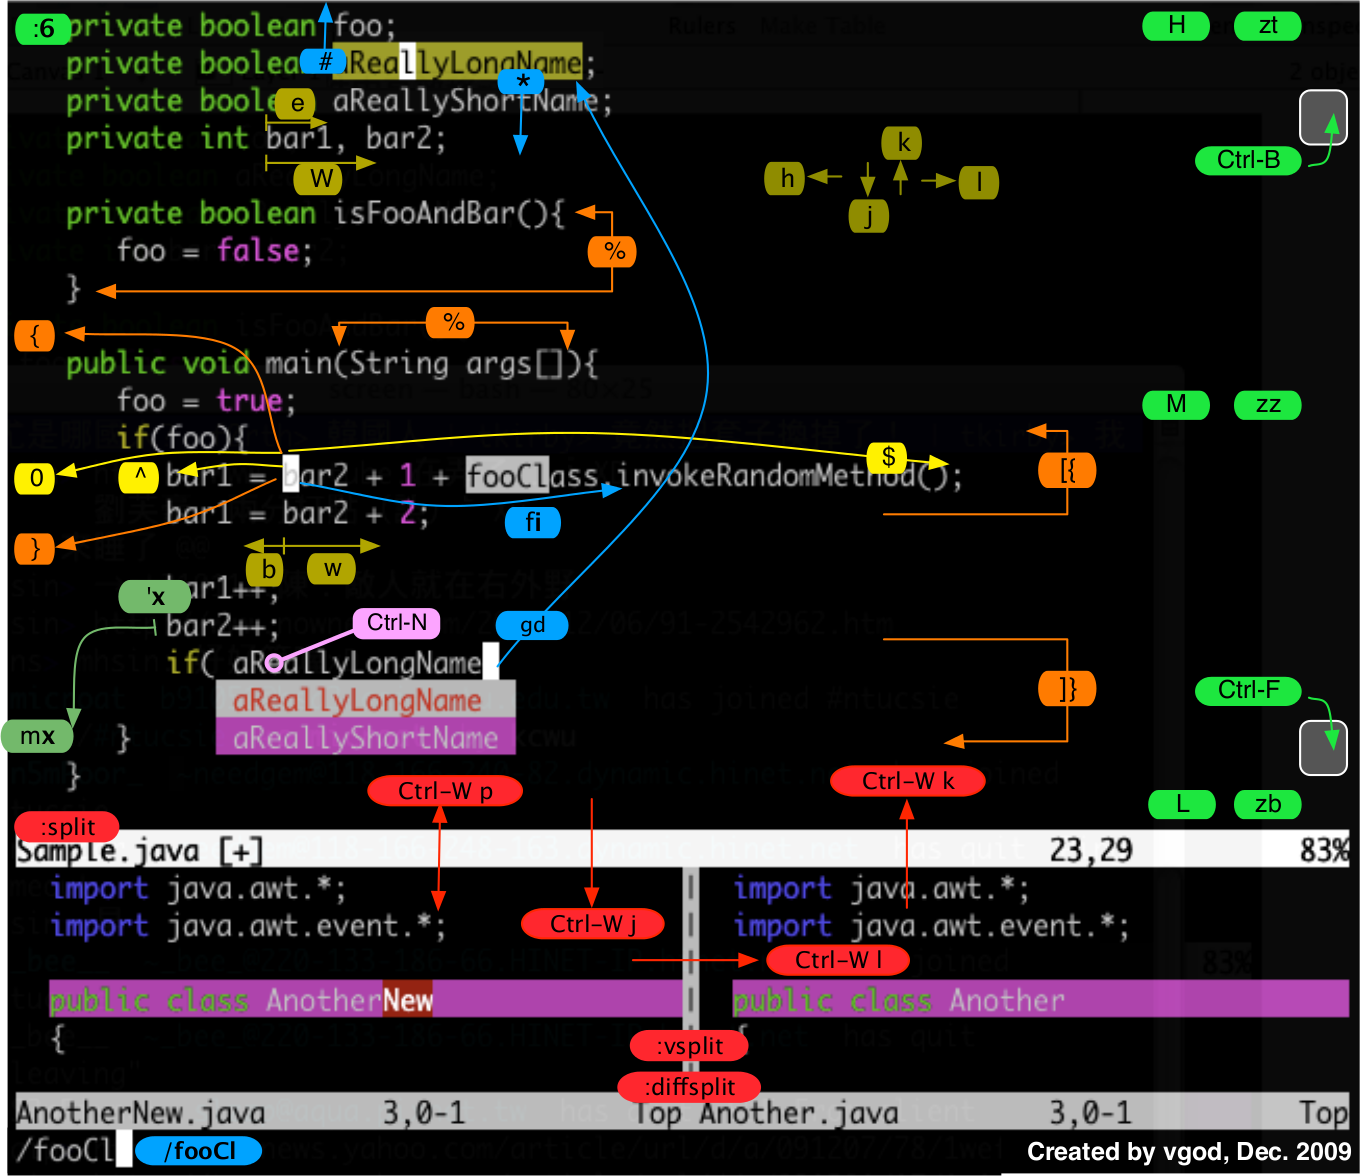
\includegraphics[scale=0.45]{vim1.png}
\end{figure}


\begin{figure}[!ht]
\centering
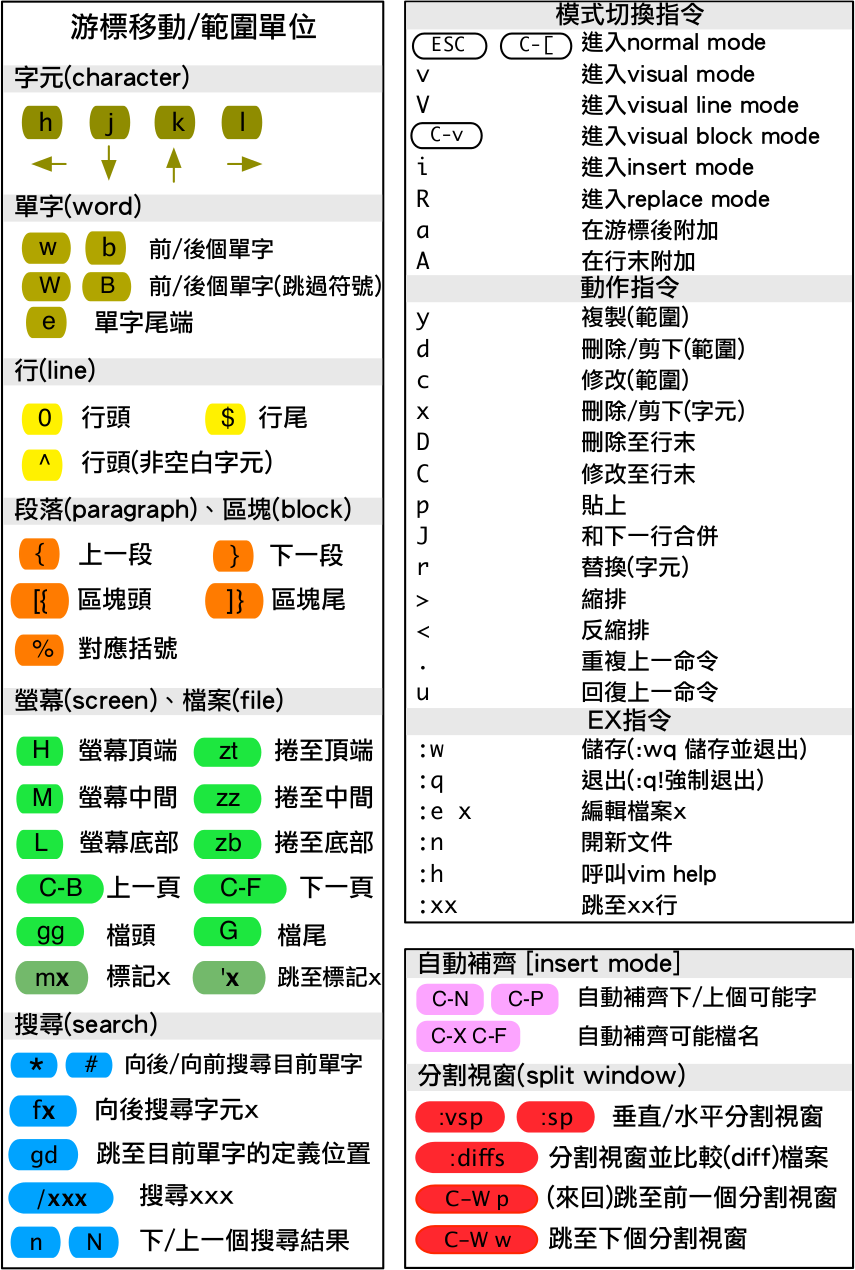
\includegraphics[scale=0.65]{vim2.png}
\end{figure}

\chapter{英雄的落幕,痞子的横行!}

\vspace{-25pt}

出处:http://blog.sina.com.cn/s/blog\_402318990100po7j.html

“在我打你右脸之时请将你的左脸伸出来,虽然我打得手疼且从骨子里头不乐意如此打人,然我还是会狠狠地给你一个巴掌。”主教这般对我说,然而我竟不乐意了,跳起来赏了他右脸一个响亮的耳光,然后又面容宛然地勒令他将自己的左脸伸到我的巴掌前面来。而原本庄严肃穆的他却变了一副垂悯可怜的样子,不知所措地看我,我突然想笑却发现自己已笑不出来,甚至连张开嘴巴的力气亦不复存在。我开始感到恐惧,为一种失去自己并涣漫与无地的恐惧。

当不成痞子我来做英雄,不想做英雄再来当痞子。这是我的句子\cite{hero_die}。

和几个人在那屋里聊天,说一女士在街上被人抢包,只怪她机灵了一些,手指力气大了一些,叫喊的声音大了一些,就那样被捅一刀死在了血泊之中。持刀者在众目睽睽之下扬长而去。聊天者四目相看几如统一方便面般道曰,事不关己,高高挂起,最多跑僻静的地方打电话报个警,而这已经是最为仁慈的做法。且不管这种做法能否救得女士的燃眉之火,这已经是冒了非常之大量的一个险。你不知道倘是持刀者知晓了你的报警行为,立刻就有性命之虞。几个人在那里唱和相随,遥相呼应,仿佛此事已了,隐隐有不复再言的样子,于是我忍不住了。拿起一把水果刀割开自己腕上的血管,看里面的血流在眼前,倒也还是红淌淌的,带了一股蒸腾的热气,并时不时地像沸腾的开水般翻滚涌簇起来。我转头看他们,他们也正诧异地看我,看我的血。于是我大笑起来,斜眼看着他们,“原来我们的血是不同的,难怪难怪,你们的血怕是冷蓝色的吧?”几人惴惴般通些眼神,“我们是什么人来着,我们都是一些安分守己持良民证的良民,哪里像你……”

我已不想再听诸多解释,摔袖起身出门。在门口,一老头拉住我的衣摆,挪动干瘪的嘴唇用了萎缩的声音说到,“年轻人,你的棱角没有磨平出去是要吃亏的。人生在世,且如蝼蚁,但为偷生,切不可枉自造次。”我站住回头看他,“你知不知道从小到大我打过几次架?”老头摇摇头,“不知道。反正我是没打过。一般别人打我时,我都打不过他们,所以我忍了。”“那在别人打你的时候有人帮你么?”于是我再问。“没有,没有……”老头放开手,一步一步退回无影之中,于是我走了出去。

公理,正义,与人。

“你知道做英雄的代价么?”他们从腰间抽出明亮的砍刀狞笑着对我,刀光晃动眼睛让我不得不偏头避过那些锋芒。

天阴沉得骇人,一如将地狱倒置般低压了这个世界。我已不想开口选择,也不想到处躲避,于是我立直身子站到地狱底下,用眼睛盯着他们的眼睛,看他们如何看我。

旁人于远处看我,用了诧异的眼神略带了些鄙夷的色彩。好出风头的家伙总会让他们感到莫名的妒忌,因为妒忌,所以他们发誓要用自己鄙夷的眼光击碎心中低劣的暗影。他们已在咀嚼玩味着我的覆灭,然而此时,他们站得很远,生怕不小心惹上血腥的味道。

于是,持刀者在将我缚住,用麻绳将我垂吊于虚无上空。围观者越来越众,在一片喧嚣之中,持刀者开始除去我的衫裤,让我用赤裸的身体对了不断停走过来的旁观之人。在一片掩口窃笑之中,没有牛皮的马鞭,持刀者兴奋地从旁野的丛中折下苦竹的一半,用浑身的力气狠狠地在我的肉身之上鞭出数以千计的血痕。在那血滴滴溅落之时,他们也正狂笑庆贺自己的胜利,顺便对着那些正嘻笑指点不止的围观者露出口中的獠牙,在惊退众人之后扔下手中带血的竹鞭放声长笑扬长而去。

然而我未死去,仍垂头用寂寞的眼神看地。那荒瘠之地,长满松蓬的野草,并未在热血的浇灌之下开出哪怕一朵的鲜花抑或显露一株的实木。人群未散去,我已在迷离中听他们仍在嘲笑着一个人赤身裸体的死亡,并指点着某一处让他们堪觉兴奋的地方。我想努力抬头,看天上或许正有飞鸟哀鸣着缀行路过,然而于那遥远天际,未曾透出一丝可见的亮光,阴郁的墨云仿似妖魔般变幻。

那些良久的愤怒。

血逐渐冷却,心亦悲哀如死般凋谢于无神之境。没有赞歌,麻绳在长久的冷漠之中腐烂以至掉落。我重新踏足于这世界,开始用接近冰封的眼神冷冷看那些人。

他们也正在涎笑看我:“我只是旁观者而已,我只是旁观者而已。何况是你自己没事找事,我们看得真是开心啊。你的那个东西好生有趣……”笑声逐渐变响变响,慢慢汇成一片放肆的笑海。

于是我陡然在那些笑中重生。穿上持刀者扔在地上的衣服,并将其中笑地最为得意的那个从人群中拖了出来用持刀者扔下的竹鞭狠狠得抽了他一顿,然后在他一地鼻涕口水黄白屎尿,哭喊哀求的声音之中扔下竹鞭,狠狠地踢了他三脚扬长而去。

“痞子,痞子……我要杀了你”我听得背后有人惶恐说到,然而终没有人敢冲上来与我搏命。

杀死英雄的不是持刀者,而是你们这些看客。我于纸上写到。而我本可于落寞的瓶中郁郁而终,是你们的笑让我重生,并以痞子的姿态横行于你们之中。佛魔之间,如此而已,如此而已。而世界,亦依旧任由那片地狱的黑暗掩覆。

每个人的惩罚,会因为你自己而到来,且在你的冷漠与笑中紧记。

后记:我需要声明,此文非本人所写,若干年前在天涯论坛一个ID为燕十三的作者写了这篇文章,当然现在此ID已经不复存在,几年后再读这文章 依然感觉不过时。

\clearpage
\bibliographystyle{plainnat}
\bibliography{gk}


\chapter{Git Cheat Sheet}


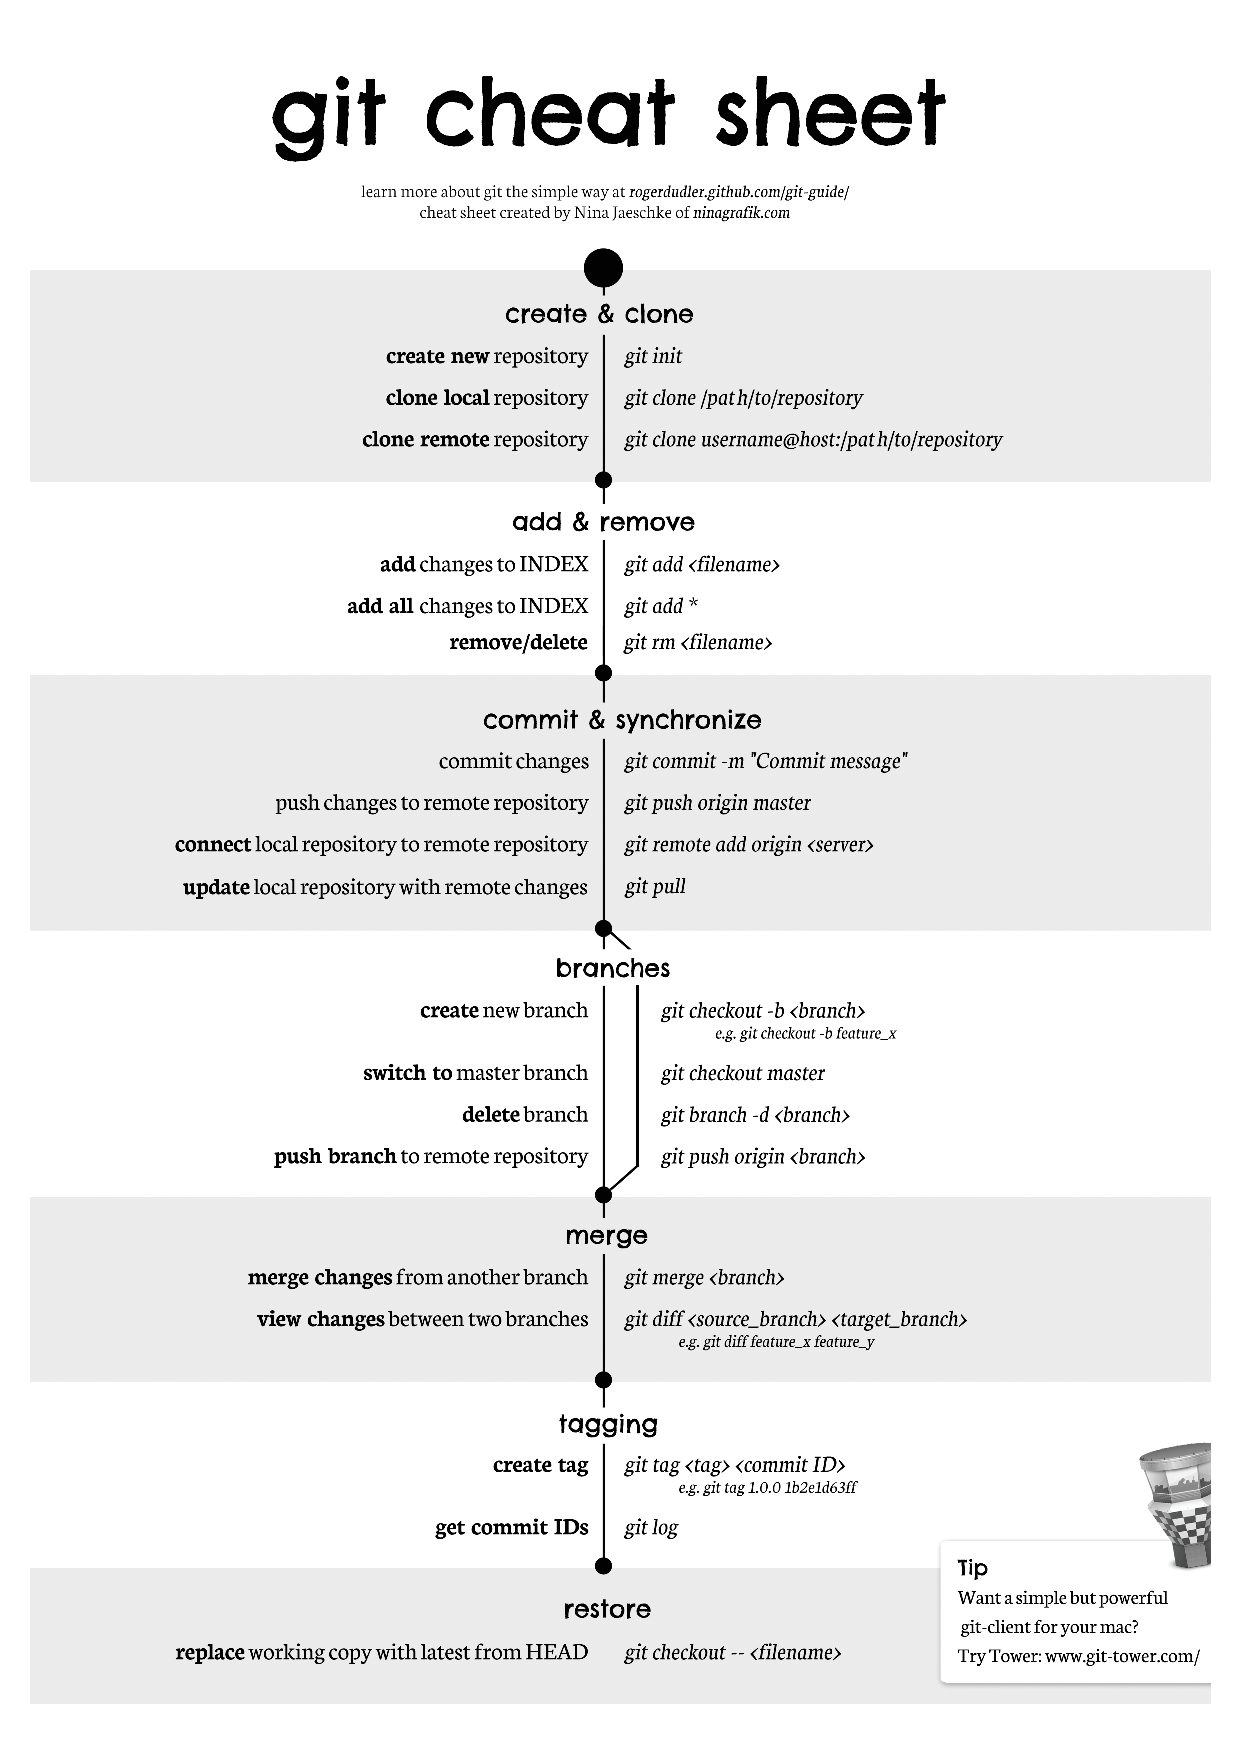
\includepdf[pages={1}]{git_cheat_sheet.pdf}

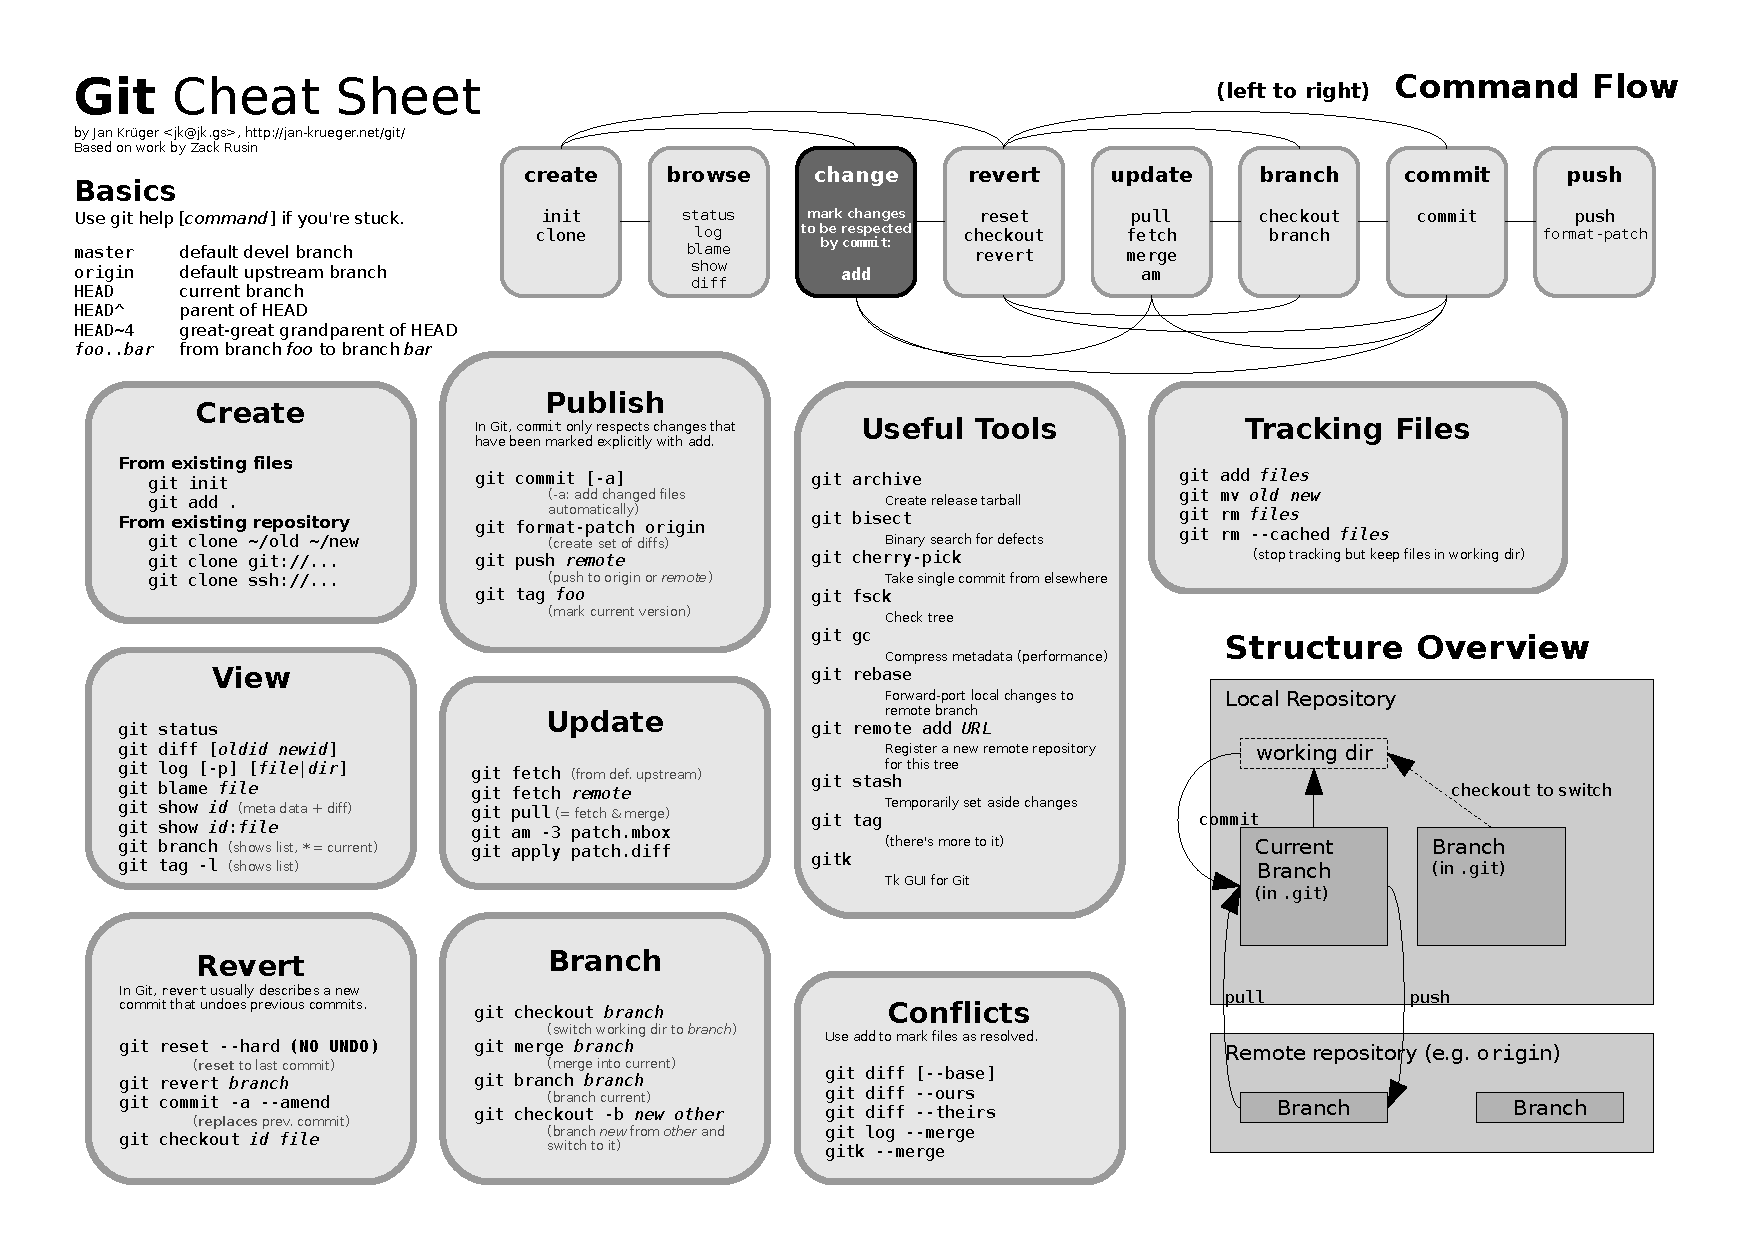
\includepdf[pages={1}]{git-cheat-sheet.pdf}

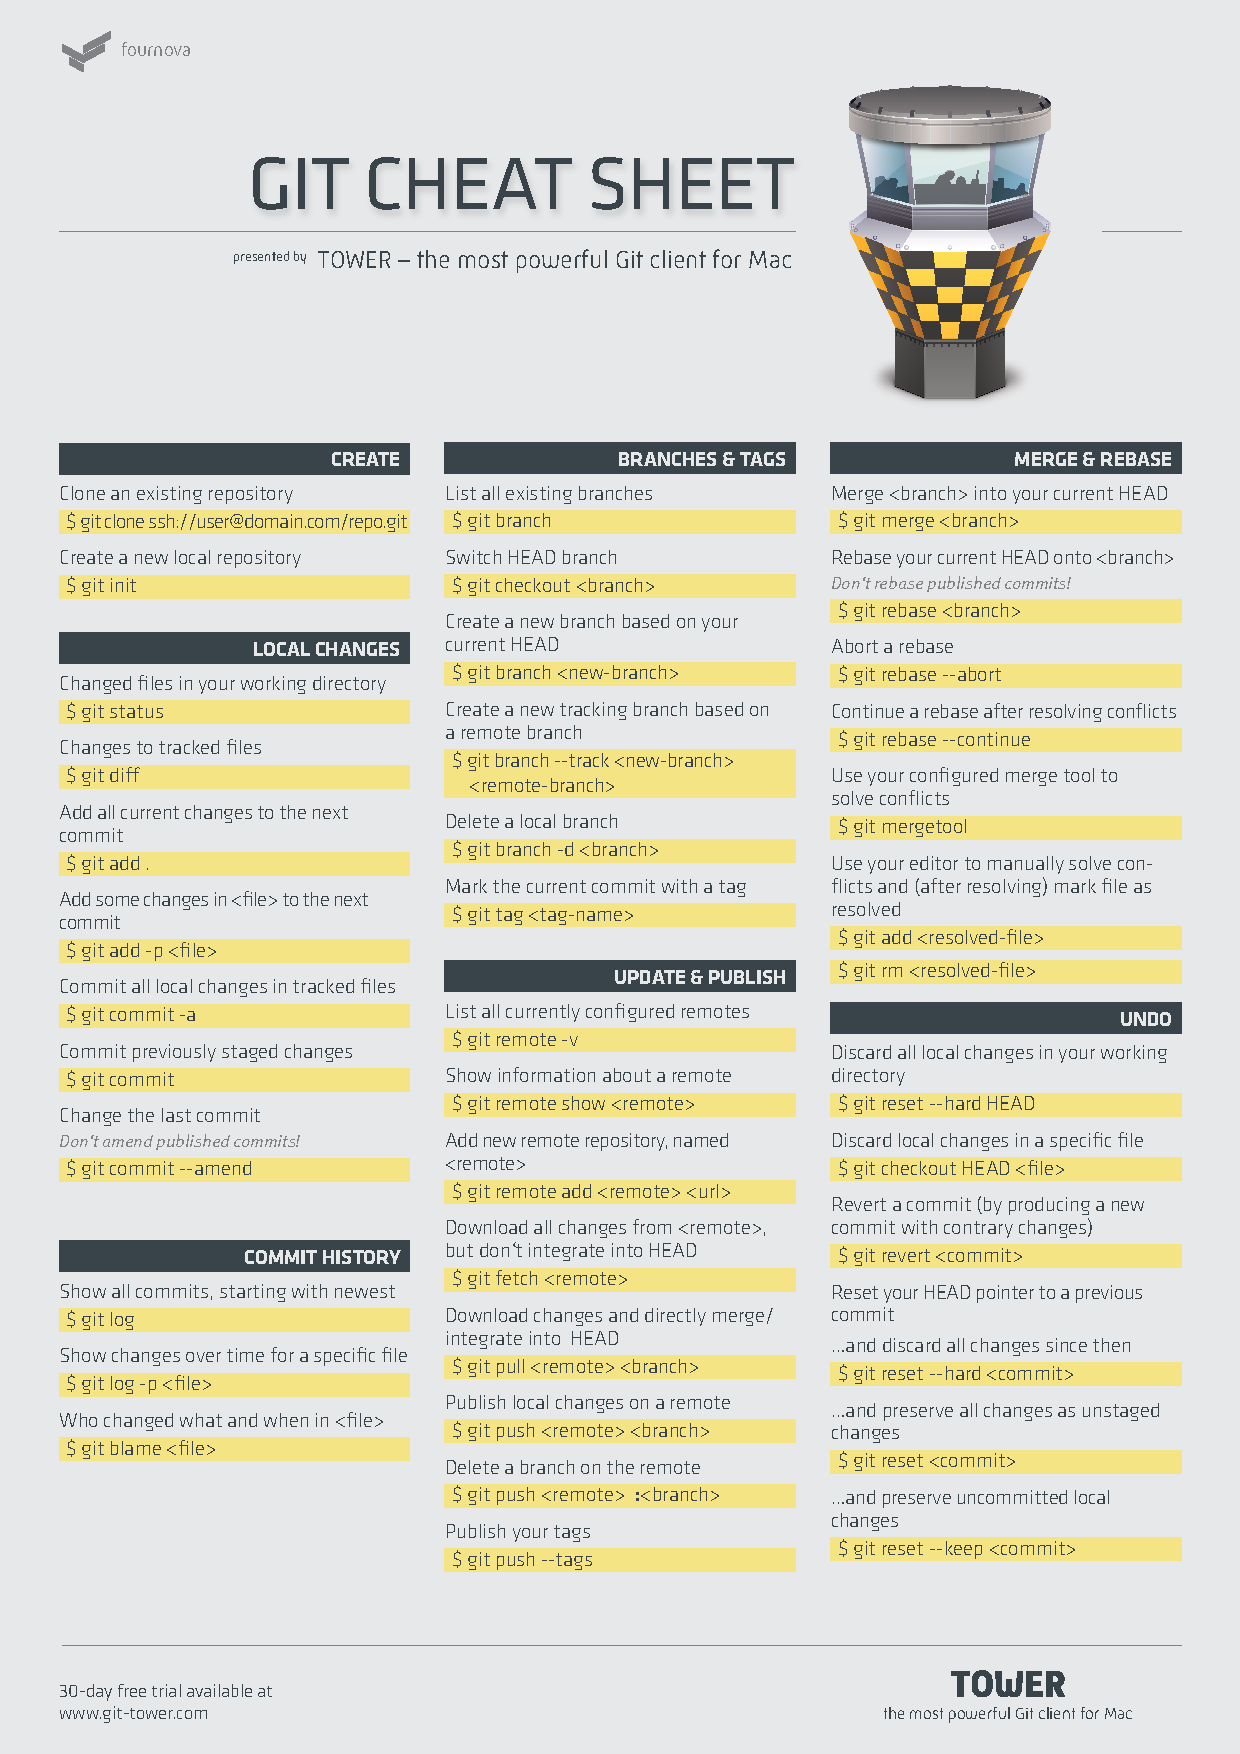
\includepdf[pages={1}]{Git_Cheat_Sheet_grey.pdf}

\chapter{Version Control Best Practices}

\includepdf[pages={2}]{Git_Cheat_Sheet_grey.pdf}

\chapter{Cheatsheet for Git as an SVN Client}

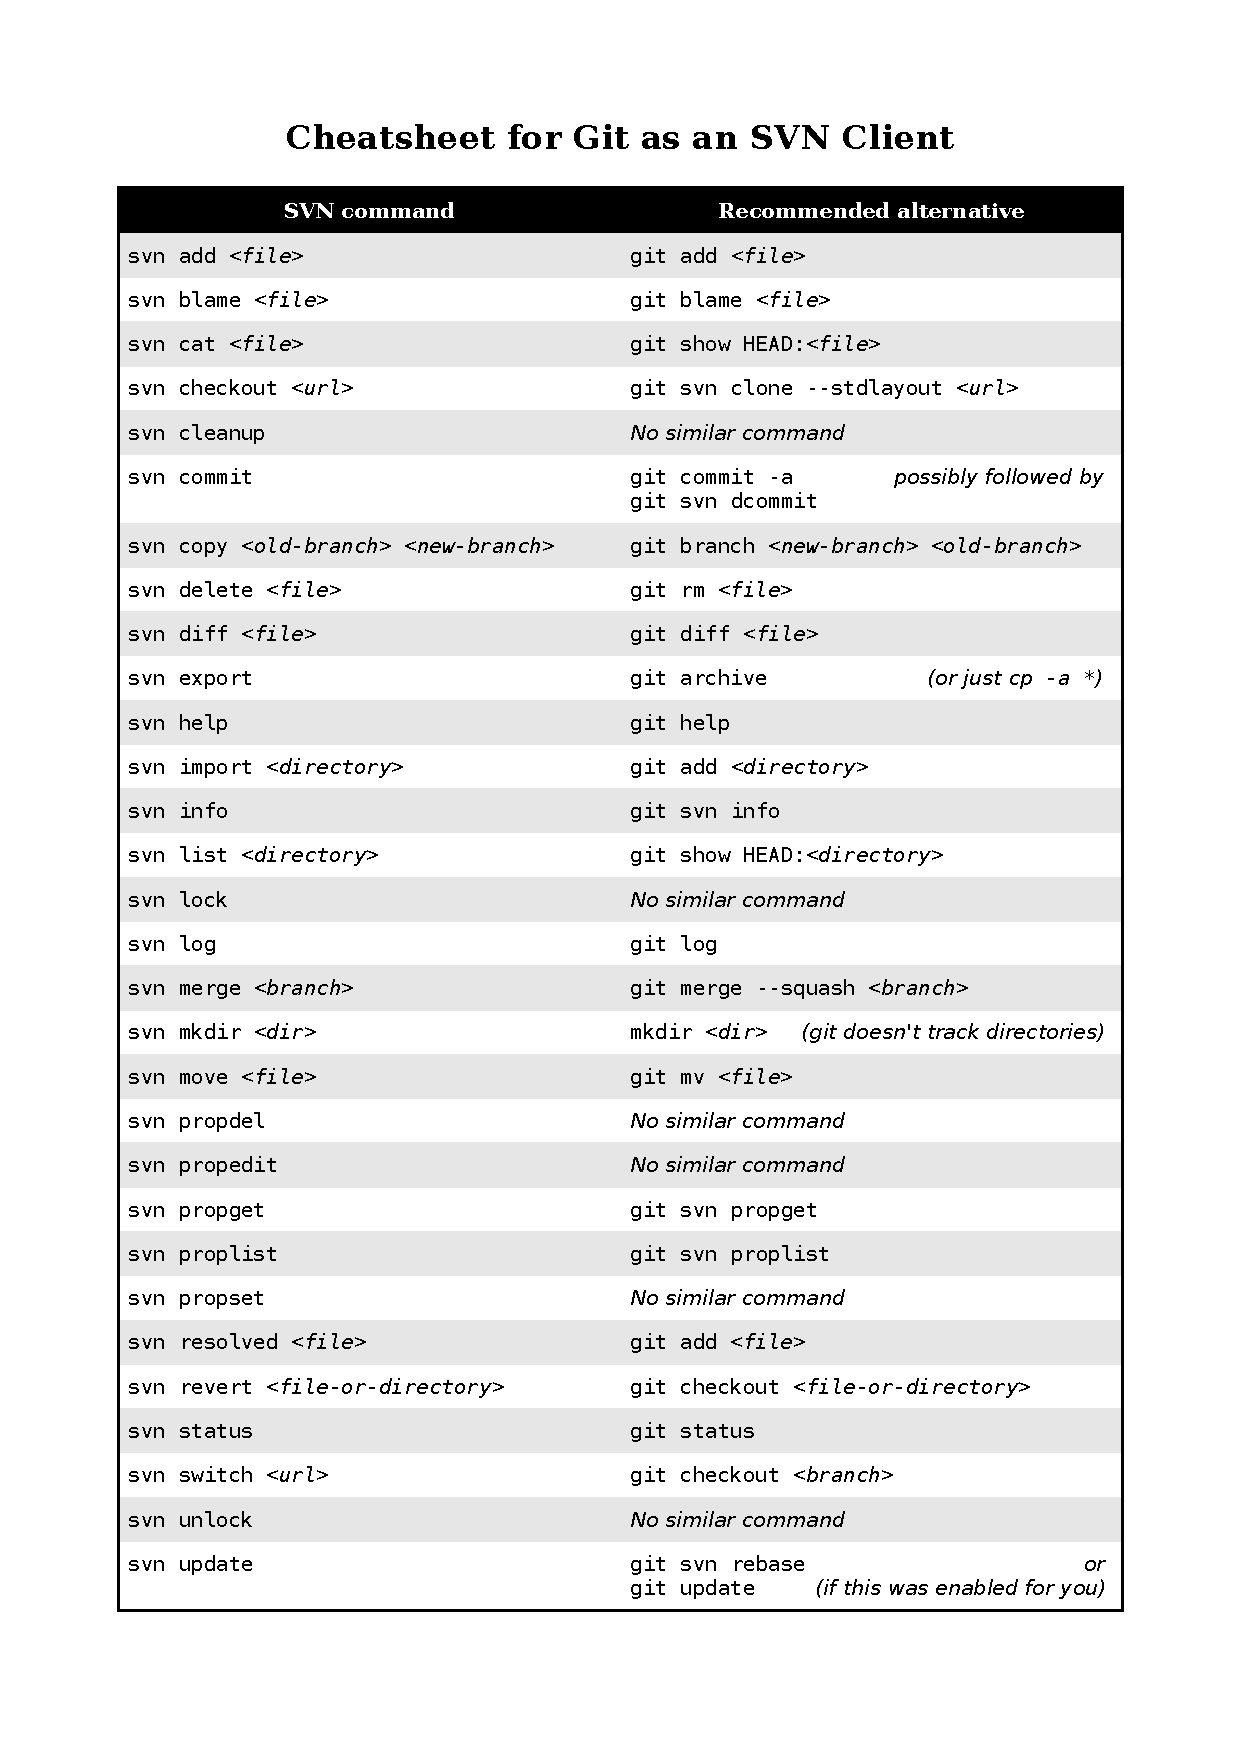
\includepdf[pages={1}]{Git-svn-cheatsheet.pdf}

\chapter{SEO}

出处:http://lutaf.com/best-seo-tutorial.htm

做站选择什么域名好

me/us/td 等后缀域名对seo有影响么

url用什么分隔符

baidu/google seo分别有什么特点

1000ip能赚多少钱

英文seo去哪里发外链

文章站的生意

英文seo

做英文seo软件大全

什么是ping

pr4的外链多少钱合适

pagerank的内幕

如何估算其它网站的流量

adsense的ctr多少

adsense的单价能到多少

mfa是什么

emd是什么

外链angel

cj是什么

cb是什么

做什么样的网站容易赚钱

黑链或者白链

如何通过SEO获取大量流量

新网站如何获取流量

英文站用什么样访问统计工具

什么样的网站是好的网站

最好的英文站长论坛列表

哪里能找到免费的网站空间

做百度seo如何发外链

如何通过seo赚钱

如何针对google做seo优化

\bibliographystyle{plainnat}
\bibliography{phpnotes}
\clearpage

\chapter{第一门编程语言选谁?}

\begin{center}
第一门编程语言选谁?\cite{first_programming_language} \\ 金旭亮
\end{center}

说明:

这篇文章是专门针对大学低年级学生(和其他软件开发初学者)写的,如果你己经是研究生或本科高年级学生,请将这篇文章转发给你的师弟或师妹,希望这篇文章能够帮助他们少走弯路,顺利地迈入软件开发的大门;如果您是一位有经验的软件开发者,或者是关注计算机教育的同行,也敬请提出宝贵意见。

发表看法请在本贴评论,或者在我的新浪微博“\href{http://weibo.com/jinxuliang}{北理工教师金旭亮}”上相互沟通。

本文仅代表个人看法,权作抛砖引玉之用。

\begin{flushright}
金旭亮写于新学期开学之际:2012年9月3日
\end{flushright}

最近,台湾知名技术专家蔡学镛先生写了一本《编程ING》,宣称“人人都能学会程序设计”。作为一名IT教育工作者,这本书引发了我的兴趣,翻看之后,共鸣之处不少,结合国内计算机教育的现状,产生了颇多感触,于是就有了这篇小文。


\section{为什么学生视编程为畏途?}

先当学生后当老师,不知不觉之中我在大学里己“混”了十多年,我发现,进入计算机专业就读的学生,最初至少有一大半对真实的软件开发根本不了解,是“一张白纸”,不幸的是,学了四年之后,许多张“白纸”又变成了许多罐“浆糊”,带着对软件开发可能是畏惧也可能是无所谓但绝对不是喜欢的感触离开校园。

编程真的那么没劲?那么难和枯燥?

我写了将近二十年的代码,虽然不靠编程吃饭,但也似乎勉强可算是个老程序员,我对编程的看法可总结为两句:何以解忧,唯有编程!我经常在想一个问题:编程其实是很有趣很好玩很实用并很有成就感的一件事,为什么会有这么多的学生视编程为畏途?而我们的计算机教育,为什么在打掉学生对编程的兴趣方面“如此成功”?

蔡学镛先生在《编程ING》给出了一张图:

\begin{figure}[!h]
\centering
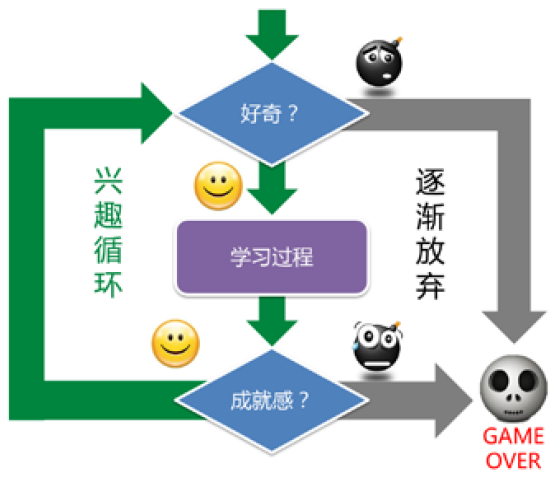
\includegraphics[scale=0.5]{bcing.png}
\caption{图1 正向兴趣循环是学习的关键}
\label{bcing}
\end{figure}

我认为这张图道出了问题的关键——学习过程中的“正向”兴趣循环是否成功地建立。

强烈的兴趣与不断获得的成就感是整个学习过程的“引擎”,它为学生完成整个学习任务提供源源不断的强大动力。有无数的事实支持这个观点。

传统的教学观点认为,本科的主要教育目标之一是为学生在本专业领域未来的发展“打下扎实的理论与实践基础”,所以从一开始就要“严格要求”,“科学训练”。

这个观点不能说错,但我认为,我们的计算机教育,尤其是针对初学者的教育,首要的任务是引发兴趣。没有兴趣,一切免谈。

我所了解的事实是:计算机专业的学生有不少视编程为畏途。其原因在于我们的现有计算机教学方式从一开始就给了这些学生“痛苦”的编程体验,不幸的是,这种体验在后期枯燥的专业课学习中不断得到强化,学生最终对编程敬而远之或畏之如虎。

事实上,教育学研究早己指出,成功的高效的教学应该是这样的:循序渐进,由浅入深,步步为营,兴趣导向。

教师的职责,不是将知识“灌入”学生的大脑,首要的任务是引发学生的兴趣,鼓励他们去探索未知的领域,主动地学习和吸收知识,培养技能,积累经验。在这个学习过程中,教师要成为一名优秀的导航员,给学生绘出航线,鼓励他们出海远航,解决他们在航行中所遇到的困难,并帮助学生建立学习的“正向”兴趣循环。

对编程的“第一印象”很重要啊!由此,引发了一个很有趣的问题——应该选择哪一门语言作为学生的第一门编程语言?

\section{你学的第一门编程语言是什么?}


在国内的大学中,当前大多数选用C作为学生的第一门编程语言。这其实并没有太大的问题,C的重要性无须我多说。其实问题的关键不在于选择C教学,而在于以哪种方式去教。

很不幸,国内许多C语言的教材都将主要的精力放在对C语法细节的介绍上,课程考核方式又很古板——很多院校采用闭卷考试,出一堆的选择题和填空题。典型的题目是将一段代码砍掉一两句,让学生“填空”。有哪位高手是通过做这些“填空题”学会编程的?上机也流于形式,让学生反复折腾几个“黑底白字”的“玩具般的”小程序,学了一个学期,学生连一个有点用的程序都写不出来……

这种僵化的教学方式,足以毁掉多数学生对编程的兴趣。

 我个人认为,C不应该成为针对大多数学生所讲授的第一门编程语言,我们的教学体系,应该给学生提供更多的选择。

针对初学者所讲授的第一门编程语言,应该具有以下的特点:

\begin{compactenum}
\item 必须是“有趣”的,能诱导人去“动手”和“思考”。
\item 需要对初学者屏蔽不必要的底层技术细节,以免分散他们的注意力。
\item 这种语言必须足够简单,但同时又具备足够的能力编写出实用的程序,从而让学生能比较容易地获得成就感,感悟到软件开发的魅力。
\item 这种语言必须能充分地体现现代软件开发的基本思想和技术成果,为学生进一步深入学习打下基础
\item 花在这门编程语言上的时间和精力是有回报的,掌握了它,就掌握了一个强大的工具,可以在今后的学习中使用这个工具进行实践和创造。
\end{compactenum}

另外,这门编程语言的学习,应该有助于初学者正确理解与体会到以下的编程思想:

\begin{compactenum}
\item 分而治之:将大问题切分为小问题。
\item 组件化与模块化:以搭积木的方式“构建”出软件系统。
\item 算法思想:针对实际问题建立数学模型,设计计算机算法,最终编程解决问题。
\end{compactenum}

同时,这门编程语言的学习,应能有效地培养出以下的编程基本功:

\begin{compactenum}
\item 调试代码的能力。
\item 撰写可读性强、扩充性好、易于复用的优质代码的能力,培养良好的编程习惯。
\item 查找技术资源与阅读技术文档的能力。
\end{compactenum}

也许一门编程语言的学习无法达到上述的所有要求,但组合几种不同的编程语言就差不多了。下面,我介绍几种适合于初学者入门的编程语言。

\section{适合于入门的脚本编程语言}

为了教初学者学会编程,蔡学镛先生的《编程ING》选择了REBOL编程语言,这个语言确实比较简单,而且蔡先生的书图文并貌,用它来训练编程的基本技能很合适,但REBOL这门语言似乎过于小众化了一些,而且书中缺乏有力的能引发初学者兴趣的应用实例。

依据我的经验,如果初学者能动手写出几个有用的实例,他喜欢上编程的可能性会大大增加。

以下是我粗略归纳的很容易引发学生成就感的几个技术领域:

\begin{compactenum}
\item 图形图像与动画、多媒体
\item 游戏
\item 网络应用
\item 拥有可视化界面的桌面应用程序
\item 能跑在手机上的应用程序
\end{compactenum}


就我个人看法,第一门语言比较适合采用脚本式的编程语言。


\subsection{Python:认识编程是怎么回事,训练基本编程技能}

国外有许多人非常推崇Python(http://www.python.org),认为它是最适合初学者学习的一门编程语言。

Python是一种动态编程语言,语法简洁易学,本身是开源的,Python程序可以运行于几乎所有主流的操作系统之上。

对于初学者而言,使用Python可以学习基本的编程知识(比如学会编写分支、循环语句),体会动态编程语言的特点,并理解类和对象等面向对象编程的基本知识。

但针对国内的实际情况,使用Python存在着一些问题:

\begin{compactenum}
\item 官方提供了一个交互式的开发环境IDLE,易于使用,但要开发拥有可视化界面的程序比较麻烦,其他厂商的开发环境也不太成熟稳定。

\item 缺少合适的中文教材,与其他语言相比,在国内应用也并不算广。  个人观点:使用Python对初学者进行基本编程技能的训练还是比较合适的,但在使用它入门之后,还必须学习其他的编程语言。
\end{compactenum}


\subsection{MATLAB和Scilab:训练算法的设计与编程实现能力}


学习、应用和设计各种算法,培养为各种问题建立数学模型的能力,这对于软件开发而言非常重要,我国己在高中数学教学中引入了算法,并将其纳入了高考的考试内容,这是件好事。

当前高中新课标数学课本中,使用的是由法国国家信息自动化研究院(INRIA)开发的Scilab(http://www.scilab.org/),这个软件与大学里流行的MATLAB高度类似,是学习算法的好工具。

比较遗憾的是,Scilab也缺少足够的中文资料,并且由于高考数学仅考察简单的算法流程图,占分很少,因此大多数的高中都不会对这块投入太大力气,学生的算法思想和数学建模能力无法得到比较充分的训练,这个任务只能留到大学来完成了。

使用Scilab或MATLAB作为第一门编程语言是完全可以的,与Python类似,Scilab或MATLAB编程采用交互式的运行方式(图2),编程语法也很简易,通过它同样能培养出基本的编程技能,特别是它们强大的数学图形功能,对学生吸引力很强,Scilab或MATLAB编程对他们数学能力与算法设计应用能力的训练无以伦比,这种能力会为学生未来在学术研究领域的发展提供强劲动力。

\begin{figure}[!h]
\centering
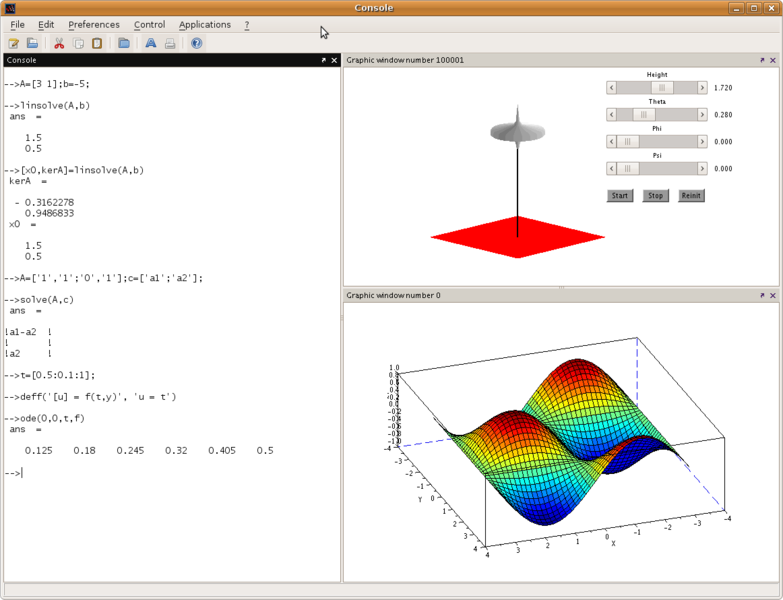
\includegraphics[scale=0.5]{scilab.png}
\caption{图2  Scilab交互式编程环境}
\label{scilab}
\end{figure}


\subsection{Office+VBA:用VBA代码控制Office,让各种工作自动化}

几乎所有大学都开设有《计算机基础》这门课程,其中大多都会讲授微软Office软件包的使用。但当前这门课程教学方式是存在问题的,比如我看到过一些考试试题,考核学生是否记住了Word的某些操作快捷键,这完全是本末倒置!其实,将本课程教学内容略作改革,完全可以用于培养学生的编程技能,其中的关键在于加强或新增以下几个内容:

\begin{compactenum}
\item 使用Excel进行数据分析,讲授Excel中功能强大的各种函数用法及数据的可视化呈现,这不仅实用,而且能有效地培养学生处理与理解数据的能力,而程序本质上不就是完成信息加工处理的工作吗?
\item 使用Access存储与检索数据,这能让学生掌握数据库使用的基础知识,形成对数据库技术的感性认识。
\item Visual BasicFor Application(VBA)编程:VBA是一种脚本式的编程语言,在Office软件包中具有“控制一切”的能力,使用它进行编程的最大好处时能让学生体会到——原来很多操作均可以一键“自动化”,并且在实现这种“自动化”的过程中拥有成就感。
\end{compactenum}

\subsection{Processing编程语言:体会图形与动画的魅力}

国内可能有很多人不知道Processing这个编程语言(http://www.processing.org/),其实它己有10多年的历史,由美国CaseyReas教授与 Ben Fry所设计,可用于构造丰富多彩的交互式应用软件。

与其它编程语言相比,Processing最强悍之处在于它的图形图像及动画编程功能。而在整个计算机技术领域中,这一块无疑是最吸引人的技术领域之一。

虽说磨刀不误砍柴功,但有不少编程语言在能够真正“砍柴(即动手开发真正有用的程序)”之前,需要太长的时间“磨刀(学习语法,掌握开发工具、阅读API文档等等)”,而Processing就不存在这个问题,它的编程语法与Java一致,但比Java简洁得多,另外,与复杂的IDE如Eclipse、Visual Studio之类相比,Processing的编程环境非常简单,这有助于学习者将主要精力用于创作上,并鼓励他们大胆地进行开发实践。

\begin{figure}[!h]
\centering
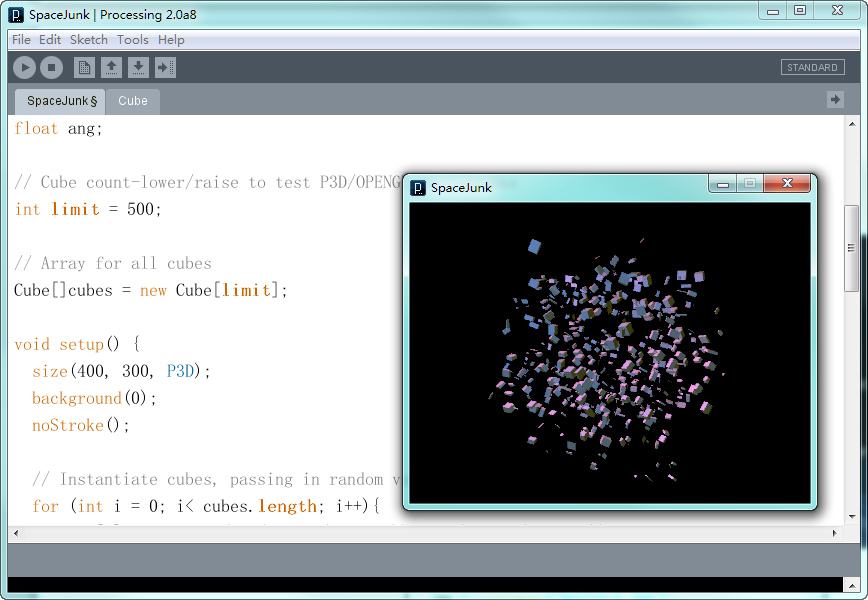
\includegraphics[scale=0.5]{processing.png}
\caption{图3 Processing编程环境}
\label{processing}
\end{figure}

Processing提供了一批直观、简洁而功能强大的图形图像函数,学习者仅需花少量时间学习就能立即投入到创作之中,而它所提供的大量可运行实例,能有效地激发学习者的想象力。

Processing具有很强的可扩展性(现在已经有一百多个库可用了),特别地,Processing内置了对于Android的支持,Processing程序能够跑在Android手机上,这大大地增加了它的吸引力。

也许不少国内高校目前还无法开设Processing课程,但事实上大学生们是完全可以自学的,Processing网站上有足够的学习资源和示例,唯一比较遗憾的是这些资源都是英文的。


\subsection{Small Basic:适合“零编程基础”人的编程语言}

在中国,有不少人是通过Basic语言迈入编程的大门的,特别是微软在上个世纪所推出的Visual Basic,更被视为Windows桌面编程最佳入门语言,只可惜这个优势在其后继版本Visual Basic.NET中己经不复存在,从功能上说,现在的Visual Basic.NET与C\#基本一致,付出的代价是Visual Basic.NET语言本身的复杂程度也变得与C\#是同一级别的了,而后者的使用者要比前者多得多,与其学Visual Basic.NET,不如直接学C\#。

这里,我想介绍的是微软所推出的另一种Basic编程语言——SmallBasic(http://www.smallbasic.com/)。

微软公司在其软件用户友好性方面一直做得非常出色,Small Basic沿袭了这个特色,其开发环境的易用性超过前面介绍的所有编程语言,并提供智能的编程帮助(图4)。

\begin{figure}[!h]
\centering
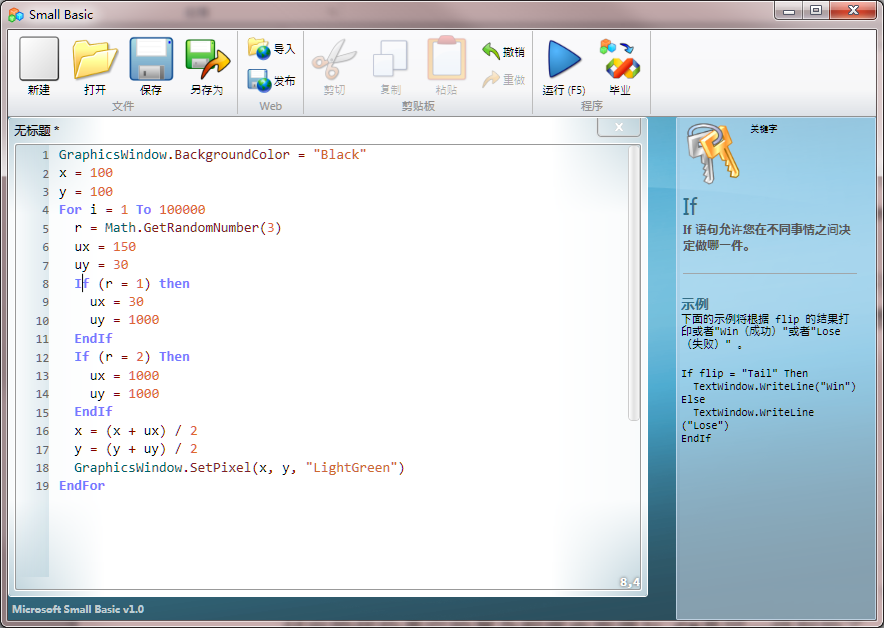
\includegraphics[scale=0.5]{small_basic.png}
\caption{图 4 Small Basic的智能编程环境}
\label{small_basic}
\end{figure}

Small Basic提供了两个强大的“窗口”对象——TextWindow(用于输出文本)和GraphicsWindow(用于绘图),特别有趣的,它从历史悠久的Logo语言中得到借鉴,提供了一个小乌龟(Turtle)对象,通过简单的指令就可以命令这只小乌龟(Turtle)在屏幕上“爬”出各种图案来,确实有趣好玩。

我个人看法,Small Basic是一个非常好的针对“零基础”人的入门编程语言,特别适合于年纪较小的学习者(比如初高中学生),也可供非计算机专业(比如文科专业)的大学生编程快速入门。


\subsection{HTML 5 + JavaScript:互联网时代的主流编程语言}

各种脚本编程语言中,我想介绍的最后一种是JavaScript。

JavaScript早就是Web客户端事实上的主流编程语言,它的运行环境是浏览器,当前所有的计算机和绝大部份智能手机都至少安装有一种浏览器,JavaScript程序“到处都可以运行”。

JavaScript程序的编写极为简单,就算使用Windows记事本,写上几段也不算太麻烦。

JavaScript早期存在的问题主要是各浏览器厂商自行其是,标准不统一,而且缺少必要的调试工具,但这些问题现在己大大缓解。以开发工具来说,主流的IDE纷纷加入对JavaScript程序开发与调试的支持,比如Visual Studio 2010/2012就做得很出色,另外,随着我们进入移动互联网的时代,HTML 5是唯一能被各厂商接受的标准,与此对应,JavaScript也正在走向标准化。

与Python等语言类似,JavaScript也可归入动态脚本语言的范畴,语法简单,同样支持面向对象的编程方式,但JavaScript的使用远比Python等语言广,诸如jQuery之类的各种JavaScript库如雨后春笋般地出现,其功能无所不包,甚至在服务端JavaScript也大展身手,比如一个事件驱动的服务端JavaScript运行环境——Node.js(http://nodejs.org/)就相当引人注目。

JavaScript在HTML 5规范中拥有核心的地位,可以用JavaScript完成很多的工作:

\begin{compactitem}
\item 基于canvas可编程绘制二维的图形,使用SVG通过DOM可构造交互式的应用
\item  HTML 5的audio和video元素可以播放音频和视频,所以可以用JavaScript开发多媒体应用
\item  Geolocation、Communication和WebSocket  API支持编写地理感知的互联网应用程序
\item  ……
\end{compactitem}

为了抢战先机,各大浏览器厂商都在不断地完善自己的产品,争取能支持更多的HTML 5特性,而且智能手机的两大主流操作系统iOS和Android都可以运行使用JavaScript编写的Web应用。微软也在紧跟这个潮流,在其最新的Windows 8中,可以使用JavaScript编写Metro风格的Windows 8 应用。

由此看来,JavaScript可谓是风光无限。

我强力推荐在高校中推广JavaScript课程,其实国内高校在这方面也已经有一定基础了,比如许多高校都开设有《网页设计基础》这门课程,只需更新一下课程的教学内容,加入HTML 5和JavaScript的内容,并改革教学方式(比如千万不要再采用闭卷考试的方式要学生去背各种HTML标记的含义……),就能让学生跟上时代的步伐,而且我相信JavaScript一定会比C更能吸引学生,激发他们对软件开发的兴趣。

\section{以编译型的语言作为入门级编程语言}

虽然我更趋向于使用脚本语言完成初学者的编程启蒙任务,但我们同样可以使用编译型的编程语言完成这一任务。

C就不用我多说了,相信有很多牛人是从C出来的。

另两门非常重要的编译型语言是Java和C\#,我的看法是即使不把它们当成计算机专业的第一门编程语言,至少也应该在计算机专业一、二年级安排这两个编程语言的选修课程。

下面先说说Java。



\subsection{Java:“人多势众”的主流面向对象编程语言}

据说全世界的软件开发人员中,Java程序员的总人数名列前茅。人多说明市场需求量大,Java技术应用广。

采用Java作为第一门编程语言,比较适合于计算机专业的学生,能让他们一开始就能受到面向对象编程风格与思想的熏陶,之后他们可以再倒过来去学C。而不是象现在这样,先学C再学Java,谈到C再顺便说说C++,现在许多院校开设有C++课程,其实这些年来C++应用的领域被不断地压缩,而且C++语法过于复杂,开发效率低,除了部分有需求有兴趣的学生,不适合多数学生学习。

Java入门主要分为两个阶段:一是Java语法与OOP思想的领悟,二是JDK中各个Java类及相关技术(比如多线程、序列化等)的学习。

Java是Android的主要开发语言,因此学生在入门之后,可以进一步地开发基于Android的手机应用,引导学生进入移动互联的时代,具有很强的实用性,这点往往能触发学生学习Java的强劲动力。

Java天生与“开源”两字联系在一起,掌握Java之后,学生可以迈入开源的世界,探索各种丰富的开源应用和技术的奇思妙想,这对于开拓学生的视野非常有好处,并且能直接地帮助其就业。

其实很多院校都开设了Java课程,我的建议不过就是将其提到大学一年级就讲授,并立即跟上J2EE和Android的后继课程。

\subsection{C\#:面向对象编程语言的集大成者}

作为面向对象编程语言家族的后来者,C\#有足够的机缘从前辈中汲取经验,这使得C\#成为一个面向对象编程语言的集大成者。

与Java类似,C\#比较适合作为计算机专业的入门级编程语言。C\#开发通常使用微软自己研发的Visual Studio,与其他IDE相比,我认为Visual Studio是非常优秀的集成开发环境,即使是免费的版本,也拥有高度的智能性和良好的使用体验。

笔者曾经做过试验,直接带领计算机专业一年级学生在没有学C的前提下学习C\#,也开设过全校的通识选修课,针对非计算机专业的学生讲授C\#编程语言与.NET编程技术,都得到了良好的反馈。

以下是我总结出来的C\#编程中几个很能引发学生兴趣的内容:

\begin{compactenum}
\item Windows Forms:可让学生迅速地开发出可视化的桌面应用程序,极具成就感。
\item GDI+:通过简单的循环、递归的编程技巧,能够绘出漂亮的图案,并且可以移植到Web上,很吸引学生。
\item ADO.NET:掌握它学生就可以开发简单的数据库应用程序,真正地写出一些有用的程序。
\item Socket编程:让学生轻易地实现两台计算机互相交换信息,这个过程充满探索的乐趣。
\end{compactenum}

以上几板斧下来,实践证明,能成功地引发很多学生对编程的兴趣,甚至“引诱”了不少学生决定跨专业报考计算机专业的研究生。

与Java相比,C\#的问题是与微软公司绑得太紧,容易把学生局限于微软所构建的生态系统之中,影响其视野的开阔性。

就我个人观点,计算机专业的学生应该在大一,最晚推迟到大二,就掌握一门主流的通用型编程语言和开发工具(Java和C\#是我当前推荐的两种编程语言),并且在今后的专业学习中,使用它们把在后继计算机专业课中学到的理论知识应用于实践。这样一来,编程语言的学习就给计算机专业理论课的学习以强劲的推动,而学生的开发能力也将随着开发实践的深入而不断增强,为其日后迈入业界或进入学术领域铺路。

\section{结束语:与时俱进的计算机教学}

计算机是进步最快的技术领域之一,这就要求我们的计算机教学应该与时俱进并不断地调整。笔者从《计算机学会通讯》2012年第6期的一篇文章了解到,美国加州大学伯克利分校己经开设了这样的课程:教学生使用Ruby On Rails之类的工具进行敏捷开发并在Amazon web Services上部署。

“云计算”来了!

 “云计算”时代的来临,会对计算机教学的方式产生巨大的影响,笔者设想了一下,如果由教育部牵头,由国家投资支持组建一个“教育与科研云”,打造一个国家级的教育公共平台,不走商业化的路,坚持让所有的在校学生和教师都能免费使用,努力推动各种的教学资源上移到云端,让更多的课程能用上云平台所提供的丰富资源与强大计算能力,这将是一项利国利民的教育基础设施建设,从长远来说,对人的教育投资,是收益最大的投资。已经成为世界第二大经济体的中国,难道还拿不出这笔钱和资源进行这个旨在为整个民族赢得未来的长线投资?

21世纪是人类信息技术突飞猛进并全面渗透到人类社会各领域的时代,在这样一个日益信息化的时代里,

\bibliographystyle{plainnat}
\bibliography{gk}
\clearpage











\end{document}


























